\documentclass[11pt,a4paper]{article}

% ---------------------------------------------------------------------
%  TFPT --- Introduction / status assessment (English, with visualisations)
%  The compiler closure of TFPT: status assessment and reading guide
% ---------------------------------------------------------------------
\usepackage[T1]{fontenc}
\usepackage[utf8]{inputenc}
\usepackage[english]{babel}
\usepackage{lmodern}
\usepackage[a4paper,margin=2.3cm]{geometry}
\usepackage{amsmath,amssymb,amsthm}
\usepackage{booktabs}
\usepackage{tabularx}
\usepackage{multirow}
\usepackage{enumitem}
\usepackage{xcolor}
\usepackage{tikz}
\usepackage{xltabular}
\usetikzlibrary{positioning,arrows.meta,fit,backgrounds,calc,shapes.geometric,shapes.misc}
\usepackage[most]{tcolorbox}
\usepackage{microtype}
\usepackage{needspace}
\usepackage[hidelinks,colorlinks=true,linkcolor=blue!55!black,urlcolor=blue!55!black]{hyperref}

% ---- colours / boxes ----
% ---------------------------------------------------------------------
%  tfpt_style.tex -- THE shared visual style for every TFPT document.
%  Single source for colours, status markers, marker key, the \veri
%  script reference, the tcolorbox families, and the running
%  header/footer.  \input AFTER xcolor + tcolorbox[most] + hyperref are
%  loaded (every paper loads those).  Each document sets its short
%  running title before \begin{document}, e.g.
%        \def\TFPTdoctitle{Architecture and the E8 Compiler}
%  ---------------------------------------------------------------------
\usepackage{fancyhdr}
\usepackage{etoolbox}
\usepackage{tikz}
\usetikzlibrary{positioning,arrows.meta,fit,backgrounds,calc,shapes.geometric,shapes.misc}

% ---- single-source author / version / automatic date stamp ----
% ---------------------------------------------------------------------
%  tex-artefacts/version.tex -- single source for author list, version
%  and the automatic title-page date stamp of every TFPT document.
%  \input by tex-artefacts/tfpt_style.tex, so every paper that loads the
%  shared style automatically gets:
%     \TFPTauthors   -- the author list (use as \author{\TFPTauthors})
%     \TFPTversion   -- curated semantic version (bump per release; mirror
%                       the bump in changelog.tex)
%     \TFPTrev       -- auto build revision = git commit count, injected by
%                       build.sh into tex-artefacts/version-auto.tex
%                       (gitignored); falls back to "dev" for standalone runs
%     \TFPTdatestamp -- the title-page date line: \today + version + revision
%  build.sh also writes tex-artefacts/release-version.txt (gitignored):
%     "{TFPTversion} (rev {git commit count})" for Zenodo + release tooling.
%  Bump \TFPTversion here ONCE; it then updates in all papers at the next build.
% ---------------------------------------------------------------------
\def\TFPTauthors{Stefan Hamann \and Alessandro Rizzo}
\def\TFPTversion{5.3}
\def\TFPTrev{dev}
% build.sh regenerates the line below with the live git commit count:
\InputIfFileExists{tex-artefacts/version-auto.tex}{}{}
\def\TFPTdatestamp{\today\,\textperiodcentered\,v\TFPTversion\,(rev~\TFPTrev)}


% ---- colours (canonical TFPT palette) ----
\definecolor{tfblue}{HTML}{1F4E79}
\definecolor{tfgreen}{HTML}{1E7B45}
\definecolor{tfred}{HTML}{9B2226}
\definecolor{tfgold}{HTML}{B8860B}
\definecolor{tfgray}{HTML}{555555}

% ---- status markers (simplified 4-class display system) ----
% Reader-facing markers collapse to FOUR classes.  The fine-grained per-claim
% type (Axiom / Formal / Lattice / Numerical / Identity / Physical) stays in
% verification/status_ledger.csv -- the single source of truth -- so no fidelity
% is lost; the papers just show the coarse class so a reader is not overwhelmed.
%   [E] exact / machine-proven  (identity, Lie/lattice, formalised, numerical FP)
%   [C] conditional             (physical / bridge / readout, under named hypotheses)
%   [O] open / axiom            (declared input or genuine gap)
%   [X] kill test               (falsifiable threshold)
\newcommand{\mE}{{\small\textcolor{tfgreen!70!black}{\textbf{[E]}}}}
\newcommand{\mC}{{\small\textcolor{tfgold!78!black}{\textbf{[C]}}}}
\newcommand{\mO}{{\small\textcolor{tfred!80!black}{\textbf{[O]}}}}
\newcommand{\mX}{{\small\textcolor{tfred!58!black}{\textbf{[X]}}}}
% backward-compatible aliases: the old fine-grained names now render their class,
% so any not-yet-rewritten call site (or the standalone changelog) still compiles.
\newcommand{\tI}{\mE}\newcommand{\tL}{\mE}\newcommand{\tF}{\mE}\newcommand{\tN}{\mE}
\newcommand{\tIalg}{\mE}\newcommand{\tInum}{\mE}
\newcommand{\tP}{\mC}\newcommand{\tB}{\mC}\newcommand{\tR}{\mC}
\newcommand{\tA}{\mO}
\newcommand{\tX}{\mX}

% compact marker legend, placed under a marker-bearing table
\newcommand{\markerkey}{\par\vspace{1.5pt}\noindent{\scriptsize\itshape
  \textcolor{black!58}{Marker key:\ \mE~exact / machine-proven\,$\cdot$\,%
  \mC~conditional (holds under named hypotheses)\,$\cdot$\,%
  \mO~open / axiom\,$\cdot$\,\mX~falsifiable kill test.\ \
  Per-claim fine type in \texttt{verification/status\_ledger.csv}.}}\par\vspace{2pt}}

% horizontal badge bar (place once near the front of a document)
\newcommand{\TFPTbadges}{\par\noindent
  \fcolorbox{tfgreen!55!black}{tfgreen!8}{\scriptsize\mE\,exact / machine-proven}\hfill
  \fcolorbox{tfgold!70!black}{tfgold!10}{\scriptsize\mC\,conditional}\hfill
  \fcolorbox{tfred!75!black}{tfred!8}{\scriptsize\mO\,open / axiom}\hfill
  \fcolorbox{tfred!60!black}{tfred!6}{\scriptsize\mX\,kill test}\par\vspace{3pt}}

% inline reference to the script that machine-checks a claim (see verification/)
\newcommand{\veri}[1]{\,{\footnotesize\textcolor{tfblue!70!black}{[\,\texttt{verification/#1}\,]}}}
% lightweight inline colour-mark for a bare verification-script token in running
% prose / tables, e.g. \vref{v108}, \vref{v49}/\vref{v71}.  Same blue as \veri so a
% reader instantly sees "this is a machine-checked module reference".
\newcommand{\vref}[1]{\textcolor{tfblue!72!black}{\textsf{#1}}}

% ---- tcolorbox families (one visual language across all documents) ----
% keybox  : the central claim / reading of a section (blue)
% winbox  : an established result / closure (green)
% gapbox  : an open gate / honest caveat / kill criterion (red)
% auditbox: a recorded audit fingerprint, not load-bearing (gold)
% navbox  : a light, neutral navigation / reference card (document map, etc.)
% Visual language (deliberately light): a faint tint, a thin coloured frame
% and a light title band with dark coloured title text -- NOT a heavy
% white-on-saturated-colour bar -- so a page never reads as a wall of boxes.
\newtcolorbox{keybox}[1][]{enhanced,breakable,boxrule=0.5pt,arc=1.5pt,
  colback=tfblue!4!white,colframe=tfblue!70!black,coltitle=tfblue!88!black,colbacktitle=tfblue!12!white,
  fonttitle=\bfseries\small,fontupper=\small,title={#1},left=2mm,right=2mm,top=1mm,bottom=1mm}
% non-breaking variant (front-matter cards that should never split across a page)
\newtcolorbox{keyboxnb}[1][]{enhanced,breakable=false,boxrule=0.5pt,arc=1.5pt,
  colback=tfblue!4!white,colframe=tfblue!70!black,coltitle=tfblue!88!black,colbacktitle=tfblue!12!white,
  fonttitle=\bfseries\small,fontupper=\small,title={#1},left=2mm,right=2mm,top=1mm,bottom=1mm}
\newtcolorbox{winbox}[1][]{enhanced,breakable,boxrule=0.5pt,arc=1.5pt,
  colback=tfgreen!5!white,colframe=tfgreen!65!black,coltitle=tfgreen!50!black,colbacktitle=tfgreen!14!white,
  fonttitle=\bfseries\small,fontupper=\small,title={#1},left=2mm,right=2mm,top=1mm,bottom=1mm}
\newtcolorbox{gapbox}[1][]{enhanced,breakable,boxrule=0.5pt,arc=1.5pt,
  colback=tfred!4!white,colframe=tfred!70!black,coltitle=tfred!75!black,colbacktitle=tfred!12!white,
  fonttitle=\bfseries\small,fontupper=\small,title={#1},left=2mm,right=2mm,top=1mm,bottom=1mm}
% non-breaking variants (callouts that must stay whole on one page, embedded in text)
\newtcolorbox{winboxnb}[1][]{enhanced,breakable=false,boxrule=0.5pt,arc=1.5pt,
  colback=tfgreen!5!white,colframe=tfgreen!65!black,coltitle=tfgreen!50!black,colbacktitle=tfgreen!14!white,
  fonttitle=\bfseries\small,fontupper=\small,title={#1},left=2mm,right=2mm,top=1mm,bottom=1mm}
\newtcolorbox{gapboxnb}[1][]{enhanced,breakable=false,boxrule=0.5pt,arc=1.5pt,
  colback=tfred!4!white,colframe=tfred!70!black,coltitle=tfred!75!black,colbacktitle=tfred!12!white,
  fonttitle=\bfseries\small,fontupper=\small,title={#1},left=2mm,right=2mm,top=1mm,bottom=1mm}
\newtcolorbox{auditbox}[1][]{enhanced,breakable,boxrule=0.5pt,arc=1.5pt,
  colback=tfgold!7!white,colframe=tfgold!70!black,coltitle=tfgold!45!black,colbacktitle=tfgold!16!white,
  fonttitle=\bfseries\small,fontupper=\small,title={#1},left=2mm,right=2mm,top=1mm,bottom=1mm}
\newtcolorbox{navbox}[1][]{enhanced,breakable,boxrule=0.5pt,arc=1.5pt,
  colback=tfgray!3!white,colframe=tfgray!55,coltitle=tfgray!30!black,colbacktitle=tfgray!12!white,
  fonttitle=\bfseries\small,fontupper=\small,title={#1},left=2mm,right=2mm,top=1mm,bottom=1mm}
% back-compatibility aliases (older box names map onto the canonical types)
\newtcolorbox{audbox}[1][]{enhanced,breakable,boxrule=0.5pt,arc=1.5pt,
  colback=tfgold!7!white,colframe=tfgold!70!black,coltitle=tfgold!45!black,colbacktitle=tfgold!16!white,
  fonttitle=\bfseries\small,fontupper=\small,title={#1},left=2mm,right=2mm,top=1mm,bottom=1mm}
\newtcolorbox{resbox}[1][]{enhanced,breakable,boxrule=0.5pt,arc=1.5pt,
  colback=tfgreen!5!white,colframe=tfgreen!55!black,coltitle=tfgreen!50!black,colbacktitle=tfgreen!12!white,
  fonttitle=\bfseries\small,fontupper=\small,title={#1},left=2mm,right=2mm,top=1mm,bottom=1mm}
\newtcolorbox{roadbox}[1][]{enhanced,breakable,boxrule=0.5pt,arc=1.5pt,
  colback=tfgreen!5!white,colframe=tfgreen!55!black,coltitle=tfgreen!50!black,colbacktitle=tfgreen!12!white,
  fonttitle=\bfseries\small,fontupper=\small,title={#1},left=2mm,right=2mm,top=1mm,bottom=1mm}
\newtcolorbox{intbox}[1][]{enhanced,breakable,boxrule=0.5pt,arc=1.5pt,
  colback=tfgold!7!white,colframe=tfgold!70!black,coltitle=tfgold!45!black,colbacktitle=tfgold!16!white,
  fonttitle=\bfseries\small,fontupper=\small,title={#1},left=2mm,right=2mm,top=1mm,bottom=1mm}

% ---- colour-marked display formula (load-bearing key equations) ----
% A highlighted formula line: a coloured left accent bar + faint tint, no full
% frame -- so a key equation is visually set apart from the running prose
% without becoming yet another box.  Use:  \begin{keyeq}$\displaystyle ...$\end{keyeq}
\newtcolorbox{keyeq}{blanker,breakable=false,halign=center,
  colback=tfgold!8!white,borderline west={2.4pt}{0pt}{tfgold!75!black},
  left=8pt,right=6pt,top=3pt,bottom=3pt,before skip=5pt,after skip=5pt}

% ---- running header / footer (consistent across all documents) ----
\providecommand{\TFPTdoctitle}{}
\setlength{\headheight}{14pt}
\pagestyle{fancy}
\fancyhf{}
\fancyhead[L]{\footnotesize\textcolor{tfgray}{\textit{TFPT}\,\textbullet\,\TFPTdoctitle}}
\fancyhead[R]{\footnotesize\textcolor{tfgray}{\thepage}}
\fancyfoot[L]{\scriptsize\textcolor{tfgray}{v\TFPTversion\,\textperiodcentered\,rev~\TFPTrev}}
\renewcommand{\headrulewidth}{0.3pt}
\renewcommand{\footrulewidth}{0pt}
\fancypagestyle{plain}{\fancyhf{}\renewcommand{\headrulewidth}{0pt}%
  \fancyfoot[C]{\footnotesize\textcolor{tfgray}{\thepage}}%
  \fancyfoot[L]{\scriptsize\textcolor{tfgray}{v\TFPTversion\,\textperiodcentered\,rev~\TFPTrev}}}

% ---- shared figure macros (claim stack, anchor cockpit, E8 glue, 2/3 motif, K5) ----
%  (this fragment lives in tex-artefacts/ and is \input by documents compiled from
%   the repository root, so the path is given relative to that root.)
% ---------------------------------------------------------------------
%  tfpt_figures.tex -- shared, reusable TikZ figure macros for every
%  TFPT document.  \input by tfpt_style.tex (which loads tikz + the
%  needed libraries + etoolbox).  Each macro draws a self-contained
%  centred figure; nothing is drawn until the macro is called.
%
%    \TFPTclaimstack[zone]  -- the architecture claim stack (B3); the
%                              optional zone in {axioms,anchor,compiler,
%                              sm,bridges,frontier} is highlighted.
%    \TFPTanchorcockpit      -- the anchor a=(1,1,2) cockpit (B4)
%    \TFPTeightglue          -- the D5 (+) A3 +mu4 => E8 glue (B5)
%    \TFPTmotif              -- the 2/3 motif map (B6)
%    \TFPTactionkfive        -- the K5 action-lattice mnemonic (B7)
% ---------------------------------------------------------------------

% ===== B3: the architecture claim stack =========================
\newcommand{\tfhl}[1]{\ifdefstring{\tfcur}{#1}{cbhi}{cbnl}}
\newcommand{\TFPTclaimstack}[1][none]{%
\def\tfcur{#1}%
\begin{center}
\begin{tikzpicture}[font=\footnotesize,
  cb/.style={rounded corners=2pt,inner sep=4pt,text width=118mm,align=center,minimum height=8.5mm},
  cbnl/.style={line width=0.5pt}, cbhi/.style={line width=1.5pt},
  ar/.style={-{Stealth[length=2.2mm]},tfgray,semithick}]
  \node[cb,fill=tfred!8,draw=tfred!75!black,\tfhl{axioms}] (axioms)
    {\textbf{P1}\,$c_3=\tfrac1{8\pi}$ \quad \textbf{P2}\,$g_{\mathrm{car}}=5$ \ \textcolor{tfgray}{\itshape(two inputs, [O] axioms)}};
  \node[cb,fill=tfblue!8,draw=tfblue,\tfhl{anchor},below=3.5mm of axioms] (anchor)
    {Anchor $a=(1,1,2)$:\ $e_1,e_2,e_3=4,5,2$ \ \textcolor{tfgray}{\itshape([E] exact)}};
  \node[cb,fill=tfgreen!10,draw=tfgreen!70!black,\tfhl{compiler},below=3.5mm of anchor] (compiler)
    {Discrete compiler:\ $D_5\oplus A_3+\mu_4\Rightarrow E_8$,\ $h=30$,\ $\varphi_0$ \ \textcolor{tfgray}{\itshape([E] exact)}};
  \node[cb,fill=tfgreen!7,draw=tfgreen!60!black,\tfhl{sm},below=3.5mm of compiler] (sm)
    {SM skeleton:\ three families, hypercharges, flavor matrix $R$ \ \textcolor{tfgray}{\itshape([E])}};
  \node[cb,fill=tfgold!12,draw=tfgold!80!black,\tfhl{bridges},below=3.5mm of sm] (bridges)
    {Physical bridges:\ $v_{\mathrm{geo}}$,\ $G_{\mathrm{net}}$,\ $F_{\mathrm{transfer}}$ \ \textcolor{tfgray}{\itshape([C] bridges)}};
  \node[cb,fill=tfgray!12,draw=tfgray!70!black,\tfhl{frontier},below=3.5mm of bridges] (frontier)
    {Frontier readouts:\ $\Lambda$, inflation, $\eta_B$, dark matter, QG \ \textcolor{tfgray}{\itshape([C]/[O])}};
  \draw[ar] (axioms)--(anchor); \draw[ar] (anchor)--(compiler);
  \draw[ar] (compiler)--(sm);   \draw[ar] (sm)--(bridges); \draw[ar] (bridges)--(frontier);
\end{tikzpicture}
\end{center}}

% ===== B4: the anchor cockpit ====================================
\newcommand{\TFPTanchorcockpit}{%
\begin{center}
\begin{tikzpicture}[font=\footnotesize,
  pan/.style={rounded corners=2pt,draw=tfblue!60,fill=tfblue!4,inner sep=5pt,
    text width=46mm,align=left},
  hd/.style={font=\bfseries\small,tfblue}]
  \node[pan] (e) {\textbf{elementary} $e_k(a)$\\[2pt]
     $e_1=4\to|\mu_4|$\\ $e_2=5\to g_{\mathrm{car}}$\\ $e_3=2\to|\mathbb Z_2|$\\[2pt]
     $c_3=\tfrac1{2e_1\pi}=\tfrac1{8\pi}$};
  \node[pan,right=4mm of e] (p) {\textbf{power sums} $p_n=2+2^n$\\[2pt]
     $p_0,p_1,p_2,p_3=3,4,6,10$\\ $p_1p_2p_3=240=|R(E_8)|$\\ $p_4-p_3=8=\operatorname{rank}E_8$\\
     $\Rightarrow\dim E_8=248$};
  \node[pan,right=4mm of p] (m) {\textbf{derived motifs}\\[2pt]
     $4,5,8,16,25,$\\ $30,41,120,240$\\[2pt]
     \textcolor{tfgray}{\itshape one anchor,}\\ \textcolor{tfgray}{\itshape many projections}};
  \node[hd,above=1mm of p.north] {$a=(1,1,2)$ \ \textcolor{tfgray}{\footnotesize\itshape[E]}};
\end{tikzpicture}
\end{center}}

% ===== B5: the E8 glue ===========================================
\newcommand{\TFPTeightglue}{%
\begin{center}
\begin{tikzpicture}[font=\footnotesize,
  d/.style={rounded corners=2pt,draw=tfblue,fill=tfblue!6,inner sep=4pt,align=center,text width=36mm},
  mid/.style={rounded corners=2pt,draw=tfgold!80!black,fill=tfgold!12,inner sep=4pt,align=center,text width=52mm},
  e8/.style={rounded corners=2pt,draw=tfgreen!70!black,fill=tfgreen!10,inner sep=4pt,align=center,text width=52mm,font=\bfseries},
  rt/.style={rounded corners=2pt,draw=tfgreen!55!black,fill=tfgreen!6,inner sep=3pt,align=center,text width=52mm},
  side/.style={rounded corners=2pt,draw=tfgray!55,fill=tfgray!6,inner sep=4pt,align=left,text width=34mm,font=\scriptsize},
  ar/.style={-{Stealth[length=2mm]},tfgray,semithick}]
  \node[d] (d5) {$D_5$ discriminant\\ $\mathbb Z_4$, $q=5/4$};
  \node[d,right=10mm of d5] (a3) {$A_3$ discriminant\\ $\mathbb Z_4$, $q=3/4$};
  \node[mid,below=5mm of $(d5)!0.5!(a3)$] (glue) {$\mu_4$ anti-isometry\ ($q$-sum $=2$)};
  \node[e8,below=4mm of glue] (e8) {even unimodular $E_8$ lattice};
  \node[rt,below=4mm of e8] (rt) {$240$ roots,\ rank $8$,\ $\dim=248$};
  \node[side,right=8mm of glue] (why) {\textbf{why unique?}\\ rank $8$\\ even\\ unimodular\\ positive definite};
  \draw[ar] (d5)--(glue); \draw[ar] (a3)--(glue);
  \draw[ar] (glue)--(e8); \draw[ar] (e8)--(rt);
\end{tikzpicture}\\[2pt]
{\scriptsize\itshape $D_5\oplus A_3+\mu_4\Rightarrow E_8$ --- the unique even unimodular rank-$8$ glue \ [E] exact (lattice).}
\end{center}}

% ===== B5b: the double pushout (one glue, two categories) ========
\newcommand{\TFPTdoublepushout}{%
\begin{center}
\begin{tikzpicture}[font=\footnotesize,>={Stealth[length=2mm]},
  lat/.style={rounded corners=2pt,draw=tfblue,fill=tfblue!6,inner sep=5pt,align=center,text width=34mm},
  net/.style={rounded corners=2pt,draw=tfblue!70!black,fill=tfblue!4,inner sep=5pt,align=center,text width=34mm},
  e8l/.style={rounded corners=2pt,draw=tfgold!80!black,fill=tfgold!12,inner sep=5pt,align=center,text width=34mm,font=\bfseries},
  e8n/.style={rounded corners=2pt,draw=tfgreen!70!black,fill=tfgreen!10,inner sep=5pt,align=center,text width=34mm,font=\bfseries},
  ar/.style={->,tfgray,semithick},
  lb/.style={font=\scriptsize,text=black,align=center,fill=white,inner sep=1.5pt}]
  \node[lat] (LL) at (0,2.5)   {$D_5\oplus A_3$\\[1pt]\scriptsize root lattices,\ $\mathrm{disc}=\Z_4$};
  \node[e8l] (LR) at (6.6,2.5) {$E_8$\\[1pt]\scriptsize even unimodular,\ $\det 1$};
  \node[net] (BL) at (0,0)     {$(D_5)_1\otimes(A_3)_1$\\[1pt]\scriptsize chiral nets,\ $c=8$};
  \node[e8n] (BR) at (6.6,0)   {$(E_8)_1$\\[1pt]\scriptsize holomorphic,\ $\mu$-index $1$};
  \draw[ar] (LL)--node[lb]{$+\,\mu_4$ glue}(LR);
  \draw[ar] (BL)--node[lb]{$\rtimes\,\mu_4$ extension}(BR);
  \draw[ar] (LL)--node[lb,left=-1pt]{level-$1$}(BL);
  \draw[ar] (LR)--node[lb,right=-1pt]{level-$1$}(BR);
\end{tikzpicture}\\[2pt]
{\scriptsize\itshape One operation, two categories: the order-$|\mu_4|{=}4$ glue is the lattice pushout
$D_5\oplus A_3+\mu_4\Rightarrow E_8$ \emph{and} the simple-current / anyon-condensation extension
$(D_5)_1\otimes(A_3)_1\rtimes\mu_4\cong(E_8)_1$; the square commutes. \ [E] exact.}
\end{center}}

% ===== B6: the 2/3 motif map =====================================
\newcommand{\TFPTmotif}{%
\begin{center}
\begin{tikzpicture}[font=\footnotesize,
  ex/.style={rounded corners=2pt,draw=tfgreen!70!black,fill=tfgreen!8,inner sep=4pt,align=center,text width=92mm},
  br/.style={rounded corners=2pt,draw=tfgold!80!black,fill=tfgold!12,inner sep=4pt,align=center,text width=92mm},
  ar/.style={-{Stealth[length=2mm]},tfgray,semithick}]
  \node[ex] (a) {$|\mathbb Z_2|/N_{\mathrm{fam}}=2/3$ \ \textcolor{tfgray}{\itshape(anchor ratio)}};
  \node[ex,below=3mm of a] (b) {parabolic weights $\{0,\tfrac13,\tfrac23\}=\operatorname{spec}A_0^\star$};
  \node[ex,below=3mm of b] (c) {transfer spectrum $\{1,(2/3)^6,(1/3)^6\}$,\ gap $6\log\tfrac32$};
  \node[br,below=3mm of c] (d) {Koide target $2/3$ \ \textcolor{tfgray}{\itshape(source$\to$pole bridge [C])}};
  \node[br,below=3mm of d] (e) {Nariai / horizon entropy bound $2/3$ \ \textcolor{tfgray}{\itshape([C])}};
  \draw[ar] (a)--(b); \draw[ar] (b)--(c); \draw[ar] (c)--(d); \draw[ar] (d)--(e);
\end{tikzpicture}\\[2pt]
{\scriptsize\itshape Green: exact motif ([E]).\quad Gold: physical bridge ([C]) --- the same ratio, two epistemic types.}
\end{center}}

% ===== B7: the K5 action-lattice mnemonic ========================
%  Layout: complete graph K5 (pentagon, all 10 edges) on the LEFT, the
%  Pascal-row reading list on the RIGHT, vertically centred on the graph
%  so the two blocks never overlap.
\newcommand{\TFPTactionkfive}{%
\begin{center}
\begin{tikzpicture}[font=\scriptsize]
  % --- K5 vertices on a regular pentagon, centred at the origin ---
  \foreach \i in {1,...,5}{\coordinate (k\i) at ({90+72*(\i-1)}:12mm);}
  \begin{scope}[on background layer]
    \foreach \i in {1,...,5}{\foreach \j in {1,...,5}{\ifnum\i<\j
      \draw[tfgray!55,line width=0.5pt] (k\i)--(k\j);\fi}}
  \end{scope}
  \foreach \i in {1,...,5}{\fill[tfblue!70!black] (k\i) circle (1.8pt);}
  \node[tfgray,font=\scriptsize\itshape] at (0,-1.9) {$K_5$};
  % --- reading list, anchored to the right of the whole graph, centred ---
  \node[anchor=west,align=left,inner sep=0pt] at (1.9cm,0) {%
    $\tbinom51=5$\ \ vertices --- action $x^1$ (Hubble slot)\\[1pt]
    $\tbinom52=10$\ edges --- $\Lambda$ density pair $x^{10}$\\[1pt]
    $\tbinom53=10$\ triangles --- dual sector\\[1pt]
    $\tbinom54=5$\ \ complements --- inverse sector\\[1pt]
    $\tbinom55=1$\ \ determinant --- closure};
\end{tikzpicture}\\[2pt]
{\scriptsize\itshape $K_5$ on the five carrier slots; the action powers $x^{1},x^{5},x^{10}$ are its
$\tbinom5k$ faces \ \textcolor{tfgray}{(mnemonic; the physical scale map stays [C]).}}
\end{center}}



% ---- short macros ----
\newcommand{\cthree}{c_3}
\newcommand{\gcar}{g_{\mathrm{car}}}
\newcommand{\Nfam}{N_{\mathrm{fam}}}
\newcommand{\phiz}{\varphi_0^{\mathrm{ret}}}
\newcommand{\Oadm}{\Omega_{\mathrm{adm}}}
\newcommand{\ainv}{\alpha^{-1}}
\newcommand{\Mbar}{\bar M_{\mathrm{Pl}}}
\newcommand{\Mpl}{M_{\mathrm{Pl}}}
\newcommand{\Z}{\mathbb{Z}}
\newcommand{\PP}{\mathbb{P}}

\setlist{itemsep=2pt,topsep=3pt}
\newcolumntype{Y}{>{\raggedright\arraybackslash}X}
\emergencystretch=2.5em

\title{\vspace{-1.2cm}\textbf{Topological Fixed-Point Theory (TFPT)}\\[1.5mm]
\Large A discrete compiler for the constants of physics\\[2.5mm]
\large Two inputs --- the boundary constant $c_3=\tfrac1{8\pi}$ and a five-slot carrier --- build $E_8$\\
and read off the Standard Model: status assessment and reading guide}
\author{\TFPTauthors}
\date{\TFPTdatestamp}

\def\TFPTdoctitle{Introduction \& Reading Guide}
\begin{document}
\maketitle
\vspace{-0.8cm}

\begin{keyboxnb}[In one sentence]
\textbf{Topological Fixed-Point Theory (TFPT)} constructs, from exactly \textbf{two inputs} --- a boundary
constant $\cthree=\tfrac1{8\pi}$ (P1) and a five-slot carrier $\gcar=5$ (P2) --- a discrete compiler for
the Standard-Model skeleton: the gauge group, three families, hypercharges and the flavor matrix, with
$E_8$ ($D_5\oplus A_3+\mu_4\Rightarrow E_8$) as the consistency checksum. The \emph{algebraic core is
machine-checkable} and the dimensionless constants follow as fixed points ($\ainv=137.0359992$);
\emph{physical readouts} --- absolute scales, masses, inflation, gravity and cosmological transfers ---
run through explicitly \emph{named, status-typed bridges} ($v_{\mathrm{geo}}$, $G_{\mathrm{net}}$,
$F_{\mathrm{transfer}}$), not as free outputs. The honest one-line claim is on the status card below.
\end{keyboxnb}

% ---------------------------------------------------------------------
%  tfpt_docset.tex -- THE canonical TFPT document-set box.
%  Single source of truth for the document list; \input by the
%  introduction and every paper. Uses only universally available
%  macros (keybox + plain LaTeX math) so it compiles in every doc.
%  Each document adds its own "You are reading ..." line directly
%  after the \input.  Numbering is aligned with the file names:
%  document N == tfpt_N_*, the introduction is the entry point, and
%  R/H/O are the appendix-style companions.
% ---------------------------------------------------------------------
\begin{navbox}[The TFPT document set --- what is treated where]
\textbf{Plain language:} TFPT (Topological Fixed-Point Theory) is a small discrete compiler. Two
inputs --- the seam constant $c_3=\tfrac1{8\pi}$ and the carrier rank $g_{\mathrm{car}}=5$ --- build
$D_5\oplus A_3+\mu_4\Rightarrow E_8$ and read off the Standard-Model skeleton, the constants and the
scale grammar. The series is \textbf{the introduction plus five numbered papers and three companions},
best read in order:
\begin{enumerate}[leftmargin=2.0em,itemsep=1pt,label=\textbf{\arabic*.}]
\setcounter{enumi}{-1}
\item \texttt{introduction} --- reading guide, compiler closure, predictions, the dependency DAG and the
      single proof ledger (\texttt{verification/status\_ledger.csv}). \emph{(entry point)}
\item \texttt{tfpt\_1\_architecture\_e8} --- the two axioms, the derivation map, the EM fixed point
      $\alpha^{-1}$, the $D_5\oplus A_3+\mu_4\Rightarrow E_8$ construction, the QBL theorem chain.
\item \texttt{tfpt\_2\_standard\_model} --- the SM in one $\varphi_0$-ladder formula, flavor from
      parabolic transport (sheet diamond, dual anchor, $Q_+$ cohomology), the worked closures.
\item \texttt{tfpt\_3\_e8\_audit\_bootstrap} --- the seven $E_8$ slices as an audit raster, the cascade
      bridge, the M\"obius bootstrap.
\item \texttt{tfpt\_4\_frontier} --- honest status of $\eta_B$, $m_p/m_e$, Koide, dark matter, full QG.
\item \texttt{tfpt\_5\_redteam} --- the adversarial audit: declared attacks, what survives, what each
      reduces to, and the kill tests.
\end{enumerate}
\noindent\textbf{Companions:} \textbf{R.} \texttt{tfpt\_research\_contracts} --- the open interfaces
$(v_{\mathrm{geo}}, G_{\mathrm{net}}, F_{\mathrm{transfer}})$ as numbered contracts;
\textbf{H.} \texttt{tfpt\_horizon\_readouts} --- Appendix~H (unit-system reframe): one seam constant as
the universal horizon thermal code, the Nariai/anchor surface, the resummed seam clock;
\textbf{O.} \texttt{origin\_theory} --- why no free fundamental number remains (exact core $+$ one
honestly-typed cyclic interpretation).
\end{navbox}

\noindent\textbf{You are reading the \textbf{introduction} --- the entry point and reading guide.}

% ---------------------------------------------------------------------
%  tfpt_status.tex -- THE canonical "status at a glance" card.
%  Single source for the overall theory status; \input near the front
%  of every document so there is ONE status statement, not one per
%  paper.  Requires tfpt_style.tex (keybox, markers).  Detailed,
%  paper-specific status expansions live only where they belong
%  (introduction: five-questions + closure ledger; tfpt_4: frontier
%  table; tfpt_research_contracts: the contracts).
% ---------------------------------------------------------------------
\begin{keyboxnb}[TFPT status at a glance --- read this card the same way in every document]
\textbf{Two inputs, one compiler.} From the boundary constant $c_3=\tfrac1{8\pi}$ (axiom~P1) and the
five-slot carrier $g_{\mathrm{car}}=5$ (axiom~P2) --- jointly the elementary symmetric data of one anchor
$a=(1,1,2)$ --- the discrete compiler $D_5\oplus A_3+\mu_4\Rightarrow E_8$ is \emph{built}, and the
Standard-Model skeleton (gauge group, three families, hypercharges, the flavor matrix), the dimensionless
constants ($\alpha^{-1}=137.0359992$) and the scale grammar are read off as fixed points. The algebraic
core is machine-checked; physical readouts run through \emph{named bridges} whose status is typed below.
\smallskip\\
\noindent\textbf{What is closed, and what genuinely remains.} The discrete/algebraic layer is closed
(\mE); the everything-open residual reduces to \emph{three named interface problems}:
\begin{center}\small
\renewcommand{\arraystretch}{1.18}
\begin{tabular}{@{}lll@{}}
\toprule
\textbf{Interface} & \textbf{Question} & \textbf{Status} \\
\midrule
$v_{\mathrm{geo}}$ & the one metrology unit ($=1/\sqrt G=m/\mu$); No-Unit Thm: no compiler scale & primitive \mO \\
$G_{\mathrm{net}}$ & simple-current extension $(D_5)_1{\otimes}(A_3)_1{\rtimes}\langle(1,1)\rangle\cong(E_8)_1$ & \mE/\mC \\
$F_{\mathrm{transfer}}$ & one functor, four typed interfaces (Koide, $\eta_B$, axion, $m_p/m_e$) & \mC \\
\bottomrule
\end{tabular}
\end{center}
\noindent Everything carries a claim ID resolving to a row of \texttt{verification/status\_ledger.csv}
(the single source of truth); \textbf{if the text and the ledger ever disagree, the ledger wins.} The
historical labels $(U_{\mathrm{wall}},G_{\mathrm{metric}},F_{\mathrm{frontier}})$ are retained only for
ledger continuity --- the live residual is $v_{\mathrm{geo}}\oplus G_{\mathrm{net}}\oplus F_{\mathrm{transfer}}$.
\markerkey
\end{keyboxnb}

\TFPTbadges
\TFPTclaimstack[none]


\tableofcontents

\noindent\textbf{Reading the markers.} Claims carry one of \emph{four} reader-facing classes, so one can
see at a glance what is proven and what is conditional:
\mE\ \emph{exact / machine-proven} --- an exact identity (e.g.\ $240=16\cdot5\cdot3$), a Lie/lattice
theorem (e.g.\ $D_5{\oplus}A_3{+}\mu_4{=}E_8$), a Lean/script formalisation, or a reproduced numerical
fixed point;
\mC\ \emph{conditional} --- follows under explicitly named hypotheses (a physical bridge, readout or
pending step);
\mO\ \emph{open / axiom} --- a declared input or a genuine gap;
\mX\ \emph{kill test} --- a falsifiable threshold.
The finer per-claim type (Axiom / Formal / Lattice / Numerical / Identity / Physical) is kept in
\texttt{verification/status\_ledger.csv}, the single source of truth.

\begin{center}
\begin{tikzpicture}[font=\footnotesize,
  band/.style={rounded corners=1pt,inner sep=0pt,minimum height=6.6mm,text=white,font=\footnotesize\bfseries,align=center},
  tag/.style={anchor=west,font=\scriptsize,black!70}]
  \node[band,fill=tfgray!85,   minimum width=84mm] (b0) at (0,0.00) {Axiom --- declared inputs};
  \node[band,fill=tfblue!55!black,minimum width=70mm] (b1) at (0,0.74) {Formal --- Lean / exact script};
  \node[band,fill=tfblue,      minimum width=56mm] (b2) at (0,1.48) {Lattice --- Lie / glue / root system};
  \node[band,fill=tfgreen,     minimum width=42mm] (b3) at (0,2.22) {Numerical --- fit-free fixed point};
  \node[band,fill=tfgold,      minimum width=28mm] (b4) at (0,2.96) {Physical --- under hypotheses};
  \node[tag] at (44mm,0.00) {P1 $\cthree$, P2 $\gcar$ \quad\texttt{AX.P1.01}};
  \node[tag] at (44mm,0.74) {P2 algebra \quad\texttt{FORM.P2.02}};
  \node[tag] at (44mm,1.48) {$E_8{=}(D_5{\oplus}A_3){+}\mu_4$ \quad\texttt{E8.GLU.01}};
  \node[tag] at (44mm,2.22) {$\ainv,\Lambda,\theta_{12}$ \quad\texttt{EM.FP.01}};
  \node[tag] at (44mm,2.96) {RG masses, QG \quad\texttt{QG.AMB.01}};
\end{tikzpicture}
\end{center}
\noindent\emph{The claim stack} (bottom $=$ most certain/fewest, top $=$ conditional). Each claim sits on
exactly one level; the bottom two are inputs, the middle two are proved/reproduced, only the top is
conditional. The single source of truth for which claim sits where is
\texttt{verification/status\_ledger.csv}.

\smallskip
\noindent\textbf{No-free-pattern rule.} To keep the structure from drowning in decorative coincidences, an
identity enters the \emph{main text} only if it (1) is a necessary step in a derivation, (2) kills an
alternative, (3) is ablation-relevant, (4) links two previously independent modules, or (5) is
experimentally tested. Everything else is explicitly demoted to an \emph{audit fingerprint} \mE\ (clearly
boxed as such) --- so the load-bearing beams stay visible and the ornament never gets promoted to spine.

\noindent\textbf{Admissible-invariant classes (the harder filter).} Sharper still: a \emph{load-bearing}
integer may only come from one of seven typed sources --- (i) a symmetric function $e_k(a)$ of the anchor
$a=(1,1,2)$; (ii) a power sum $p_n(a)$ or difference $p_{n+1}{-}p_n$; (iii) a determinant, spectrum, Smith
normal form or trace of $(R,Q,K,L)$; (iv) an anchor quadratic form $u^\top M v$ with $u,v\in\{\mathbf1,a\}$;
(v) a Pl\"ucker coordinate of the anchor plane $\langle\mathbf1,a\rangle$; (vi) an $E_8$ Casimir degree or
branching block; (vii) a pre-registered experimental observable. Anything else is an audit fingerprint or a
frontier item, never spine. This is what converts TFPT from \emph{pattern hunting} (``look, another number'')
into a typed compiler: \emph{fewer admissible kinds of explanation}, not more matches.

\noindent\textbf{Reviewer path} (read in this order; the rest is support):
\begin{enumerate}[leftmargin=1.7em,itemsep=1pt]
\item the architecture: the two axioms $\{\cthree,\gcar\}$ and the two-engine picture (\S\ref{sec:docmap}, the figures);
\item the $E_8$ glue $E_8{=}(D_5{\oplus}A_3){+}\mu_4$ --- document~1, Part~II, machine-checked (\texttt{v1\_e8\_glue.py});
\item the $\alpha^{-1}$ fixed point plus ablation (\texttt{v3\_em\_alpha.py});
\item the \textbf{single status ledger} \texttt{verification/status\_ledger.csv} --- the source of truth for every claim's grade, location, dependency and script;
\item the \textbf{open gates} as numbered research contracts (\texttt{tfpt\_research\_contracts}: the residual classes R1--R5 and their current reductions) and the honest frontier list (document~4).
\end{enumerate}
\noindent Everything carries a claim ID (e.g.\ \texttt{E8.GLU.01}, \texttt{EM.FP.01}) that resolves to a row of the
ledger. \textbf{If the text and the ledger ever disagree, the ledger wins.}

% =====================================================================
\section{What this is about: the jump in construction principle}\label{sec:docmap}
% =====================================================================

\subsection*{In plain words}

\noindent\textbf{What we found.} TFPT reproduces dozens of real numbers of physics (particle masses, the
fine-structure constant, dark-energy and inflation values) from a small set of inputs --- and the
compiler closure says \emph{why} the same handful of small integers ($2,3,5,16,\dots$) reappears in
every sector: those numbers are not separate lucky hits. A single tiny ``machine'' --- fed by just
\textbf{two inputs} (a boundary number $\tfrac1{8\pi}$ and a five-slot carrier) --- builds the
exceptional symmetry $E_8$, and $E_8$ is the unimodular ``audit hull'' that classifies the discrete
Standard-Model readout: the constants, the flavor skeleton and the gravity/cosmology regime are then
read off by projection and boundary dressing (not ``printed'' for free --- where a scheme or analytic
interface is needed, it is named).

\smallskip
\noindent\textbf{Why this is simple.} There are not many separate derivations that happen to share numbers ---
there is \emph{one generator and a handful of corollaries}, and the number of independent structural
assumptions is \textbf{two}.

\smallskip
\noindent\textbf{How plausible it is.} A theory becomes more believable when it \emph{explains more from less}.
Here the two inputs are even \emph{over-determined}: the machine reproduces the very two numbers it
started from (the dashed bootstrap loop in the architecture diagram, \S2), so there is \emph{no free
dial left to tune}. The only genuinely free, continuous ingredient that remains is the number $\pi$.

\subsection*{Sharper still: one anchor $a=(1,1,2)$, and $E_8$ as a compiler hull \texorpdfstring{(\mE)}{}}

\noindent The two axioms are not even independent: they are the \emph{elementary symmetric polynomials} of the
single parabolic anchor $a=(1,1,2)$ (the exponents-at-infinity / splitting type $\mathcal O(-2)\oplus\mathcal O(-1)^2$):
\[
  e_1(a)=4=|\mu_4|,\qquad e_2(a)=5=\gcar,\qquad e_3(a)=2=|\Z_2|,\qquad
  \cthree=\frac1{2e_1(a)\pi}=\frac1{8\pi}.
\]
Its \emph{power sums} $p_n(a)=1^n{+}1^n{+}2^n=2{+}2^n$ generate the big Lie data directly:
$p_1{=}4{=}|\mu_4|$, $p_2{=}6{=}|R^+(A_3)|$, $p_3{=}10{=}\mathcal A_\Lambda$, and
\[
  |R(E_8)|=p_1p_2p_3=240,\quad \dim E_8=p_1p_2p_3+(p_4-p_3)=248,\quad p_4-p_3=8=\operatorname{rank}E_8,
\]
with the binary ladder $p_{n+1}-p_n=2^n$. So the inputs collapse from $\{\cthree,\gcar\}$ to
$\boxed{\,a=(1,1,2)\ \text{plus}\ \pi\,}$. \veri{v23\_anchor\_generator.py}
\par\smallskip
\noindent\emph{And $a$ is itself half-forced} (\mE/\mC): on $\mathbb P^1$ every bundle splits
(Birkhoff--Grothendieck), so once $|\mu_4|=4$, $\Nfam=3$, $\deg E=-4$ are set, the three positive
anti-degrees are positive integers summing to $4$, and $4=2+1+1$ is the \emph{unique} partition into three
positive parts. The genuine remaining axiom is therefore not ``why $a=(1,1,2)$'' but ``why the carrier
$\gcar=5$ / $(|\mu_4|,\Nfam)=(4,3)$'' --- that interface (with $\cthree$) is the \mO\ input layer.
\par\smallskip
\noindent\emph{Two readings, one source (no contradiction).} P1 and P2 are the \emph{operational compiler
inputs}; their anchor provenance is $a=(1,1,2)$ plus $\pi$. The \emph{single structural bedrock postulate}
is \texttt{QGEO.SYM.01} (the carrier $\mu_4$ clock is the seam's conformal deck, see
\texttt{tfpt\_research\_contracts}): it forces the $\mu_4$ deck, hence $\Nfam=3$, $\deg E=-4$ and the
tripartition $4=2{+}1{+}1$, of which $c_3$ and $\gcar$ are the two elementary readouts. ``Two inputs''
(the working axioms) and ``one postulate'' (the geometric bedrock) are the same statement at two layers.
Its geometric normal form and the mark-local$\Rightarrow\omega\circ\rho=\omega$ implication are now
Lean-formalised (\texttt{FORM.QGEO.02}/\texttt{FORM.QGEO.01}); the postulate itself stays \mO.
\par\smallskip
\noindent\emph{One source, four readings (the cleanest origin).} The four-point seam divisor $\mu_4$ on
$\PP^1$ generates the whole discrete skeleton by four canonical functors:
\[
  \underbrace{\cthree=\tfrac1{8\pi}}_{\text{thermal}}
  \quad
  \underbrace{\operatorname{rank}H_1(\PP^1\!\setminus\!\mu_4)=3=\Nfam}_{\text{cycles}\to A_3}
  \quad
  \underbrace{h^0(\PP^1,\mathcal O(\mu_4))=5=\gcar}_{\text{functions}\to D_5}
\]
\vspace{-3mm}
\[
  \underbrace{(D_5)_1\otimes(A_3)_1\rtimes\mu_4\cong(E_8)_1}_{\text{net}}
\]
and the function side even generates $D_5$ itself (\veri{v197\_rr\_carrier\_clifford\_d5.py}):
$\Lambda^{\mathrm{even}}(\mathbb C^5)=\binom50+\binom52+\binom54=16=\dim S^+$, the $\mathfrak{so}(10)=D_5$
half-spinor. So $\mu_4$ is not merely glue: it is the \emph{common source} of $A_3$, $D_5$, $\cthree$ and
$E_8$ (\veri{v189\_riemann\_roch\_carrier.py}) --- the arithmetic is exact \mE, the physical reading of the
carrier as the seam mode space stays \mC.
\par\smallskip
\noindent\textbf{What $E_8$ is (and is not).} In TFPT $E_8$ is \emph{not} an unbroken physical gauge group:
it is the unimodular \emph{audit / compiler hull} that classifies the admissible discrete charge and
residue structures. The Standard Model is a \emph{readout} after projection, not a direct $E_8$ gauge
theory; the Lorentz signature appears only after projection; fermions are not ``everything in the
adjoint''. This is exactly why the known no-go results against literal $E_8$ world-formulas
(Distler--Garibaldi; Coleman--Mandula) do \emph{not} bite: they constrain $E_8$ as a spacetime gauge
symmetry, which TFPT does not claim. The defensible claim is: \emph{TFPT is the unique parabolic
compilation of the anchor $a=(1,1,2)$ into the $E_8$ audit hull.}
\par\smallskip
\noindent In one line:
\begin{keyeq}
The anchor generates the syntax; the boundary generates the scale; $E_8$ checks the consistency.
\end{keyeq}
i.e.\ the discrete content (carrier $D_5\oplus A_3+\mu_4$, the operators $R,Q,K,L$) flows from
$a=(1,1,2)$; the continuous content ($c_3=\tfrac1{8\pi}$, $\varphi_0$, $\ainv$, the exponential scales) flows
from $\pi$; and $E_8$ is the unimodular \emph{checksum container}, not the world group.
\par\smallskip
\noindent\textbf{The anchor ratio triad (\veri{v119\_review\_validation\_2.py}).} The three elementary
symmetric values, normalised by the family count, are the theory's three recurring fractions \mE:
\[
  \frac{e_3}{p_0}=\frac23\ \text{(Koide branch / sheet ratio)},\quad
  \frac{e_1}{p_0}=\frac43\ \text{(seed gain)},\quad
  \frac{e_2}{p_0}=\frac53\ \text{(carrier branch)}
\]
--- the canonical flow's critical points are exactly $(2,5)=(e_3,e_2)$ with inflection
$\tfrac72=\tfrac{e_3+e_2}2$: the fractions $\tfrac23,\tfrac43,\tfrac53$ are not scattered numbers but the
three normalised anchor coefficients. Further micro-identities \mE:
$\Omega_{\mathrm{adm}}=2p_1p_2=48$, $10b_1=1+p_1p_3=41$,
$\Delta_Y=e_2^2=p_0^2+2\operatorname{rank}E_8=25$, $h(E_8)=e_3p_0e_2=30$,
$\operatorname{rank}E_8=p_0+e_2$.

\TFPTanchorcockpit

\subsection*{The companion documents}

\noindent The whole development is consolidated into \textbf{eight companion documents} (plus
this introduction), organised in layers that build on one another; this introduction is the entry point
and reading guide. Each document collects the material of its layer into self-contained parts:

\begin{center}\scriptsize
\renewcommand{\arraystretch}{1.25}
\begin{tabularx}{\linewidth}{@{}p{3.6cm}Y@{}}
\toprule
\textbf{Document} & \textbf{What it contains (former notes now as parts)} \\
\midrule
\texttt{tfpt\_1\_architecture\_e8} & \textbf{Core.} The two axioms $\{\cthree,\gcar\}$, the derivation map and the EM fixed point (Part~I); the Coxeter--cyclotomic compiler $\Z_{30}{=}2{\cdot}3{\cdot}5$, the explicit $D_5{\oplus}A_3{+}\mu_4$ $E_8$ construction, the machine-checkable $E_8$ appendix and the group-level glue $(\mathrm{Spin}(10){\times}SU(4))/\Delta\Z_4$ (Part~II). \\
\texttt{tfpt\_2\_standard\_model} & \textbf{Standard Model.} The full SM in one $\phiz$-ladder formula (Part~I); the flavor block from parabolic weights and the transport theorem, H2 as a spectral selector (Part~II); the worked closures --- explicit gap, APS--Fredholm, truncation/$n_s,r$, Starobinsky $M$, derived $\theta_{12}$, quark $c$, the H2 splitting type, $\Lambda$-typing (Part~III). \\
\texttt{tfpt\_3\_e8\_audit\_bootstrap} & \textbf{$E_8$ audit \& bootstrap.} The seven $E_8$ slices as an audit raster ($E_6{\times}A_2$ reads the flavor matrix) (Part~I); the old cascade $D{=}60{-}2n$ as the same even-integer spine (Part~II); the M\"obius bootstrap --- $\gcar{=}5$ and the ``$8$'' in $\cthree$ as overdetermined fixed points, only $\pi$ irreducible (Part~III). \\
\texttt{tfpt\_4\_frontier} & \textbf{Frontier.} The honest status of $\eta_B$, $m_p/m_e$, Koide, dark matter and quantum gravity --- the genuine handle, the precision, and what is \emph{not} forced onto the ladder. \\
\texttt{tfpt\_5\_redteam} & \textbf{Red Team.} The adversarial audit of the five load-bearing reductions (Targets A--E): the declared attacks, what survives each, what each one reduces to, and the explicit kill tests. \\
\texttt{tfpt\_research\_contracts} & \textbf{Research contracts.} The open gates as numbered contracts with lemma chains and closing theorems: $(U_{\mathrm{wall}})$ (now reduced to the selector triangle: $(d,n)\Rightarrow R$ columnwise, residue $=$ \emph{two} line pairings, the third integrality-forced) and $G_{\mathrm{metric}}/G_{\mathrm{net}}$ (the index-$4$ seam-net identification --- one theorem, three doors, now realised at the finite Lie level). \\
\texttt{tfpt\_horizon\_readouts} \textbf{(App.~H)} & \textbf{Appendix~H --- horizon unit system (reframe, not new physics).} One seam constant $\cthree{=}\tfrac1{8\pi}$ as the universal horizon thermal code: Hawking/de Sitter/Unruh, BH thermodynamics, Page, scrambling, Nariai bound, $v_{\rm GW}{=}c$ --- standard physics in seam units, two compiler fingerprints ($1920{=}|W(D_5)|$, $|\mu_4|{=}4$); plus the Nariai/anchor surface, the dual anchor and the resummed seam clock (\vref{v101}--\vref{v138}). \\
\texttt{origin\_theory} & \textbf{Origin Theory.} Why no free \emph{dimensionless compiler dial} remains beyond the anchor and $\pi$ (the dimensionful $v_{\mathrm{geo}}$ and transfer physics stay typed): the $(\gcar,\Nfam)$ skeleton, the triply-forced $8$, the order-$30$ Coxeter cycle, one boundary transport for flavor and horizon, the gapped unique attractor; \mE\ core plus one honestly-typed \mC\ cyclic interpretation. \\
\bottomrule
\end{tabularx}
\end{center}

\noindent The five formerly ``research-level'' problems are now \emph{closed, reduced or typed} inside the
documents where they belong --- the group-level closure $(\mathrm{Spin}(10){\times}SU(4))/\Delta\Z_4$ in
document~1 (closed), and the H2 splitting type, the Starobinsky scalaron mass, the $\theta_{12}$ texture and
the quark $c$ in document~2 (the first two closed; the quark \emph{ratios} now closed combinatorially
(\vref{v49}/\vref{v71}), only the \emph{absolute} scale a $U_{\mathrm{point}}$ anchor; $\theta_{12}$ the
seam-misalignment residual). Eight companion files (plus this introduction), each result
where it logically lives.

% =====================================================================
\section{The architecture at a glance}
% =====================================================================
The diagram below shows the whole pipeline: \emph{two} inputs on the left, the discrete compiler in the
middle, the physics on the right. Everything in between is a consequence.

\begin{center}
\begin{tikzpicture}[font=\small,
  inp/.style={rectangle,rounded corners,draw=tfred!80!black,fill=tfred!8,thick,align=center,inner sep=4pt,minimum height=10mm},
  atom/.style={rectangle,rounded corners,draw=tfblue,fill=tfblue!8,thick,align=center,inner sep=4pt},
  comp/.style={rectangle,rounded corners,draw=tfgold!80!black,fill=tfgold!12,very thick,align=center,inner sep=5pt},
  outp/.style={rectangle,rounded corners,draw=tfgreen!75!black,fill=tfgreen!8,thick,align=center,inner sep=4pt},
  ar/.style={-{Stealth[length=2.2mm]},thick,tfgray},
  back/.style={-{Stealth[length=2.2mm]},very thick,dashed,tfred!70!black}]
% inputs
\node[inp] (p1) at (0,1.2) {\textbf{(P1)} boundary\\$\cthree=\tfrac1{8\pi}$};
\node[inp] (p2) at (0,-1.2) {\textbf{(P2)} carrier\\$\gcar=5\ (3{+}2)$};
% atoms
\node[atom] (cp) at (3.4,1.2) {$C^+$: $16$ even states\\$=D_5$ half-spinor};
\node[atom] (a3) at (3.4,-1.2) {$\PP^1\!\setminus\!\mu_4$\\$=A_3$ geometry};
% compiler
\node[comp] (e8) at (7.3,0) {\textbf{Compiler}\\$\Z_{30}=2{\cdot}3{\cdot}5$\\$D_5\!\oplus\!A_3\xrightarrow{\ \mu_4\ }E_8$\\$240$ roots, $\det 1$};
% outputs
\node[outp] (sm)  at (11.2,1.7)  {Standard Model\\$\Nfam{=}3,\ \Oadm{=}48,\ b_1{=}\tfrac{41}{10}$};
\node[outp] (con) at (11.2,0.0)  {constants\\$\ainv{=}137.0359992$};
\node[outp] (cos) at (11.2,-1.7) {gravity \& cosmos\\$\Lambda,\ A_s,\ H_0$};
\draw[ar] (p1)--(cp); \draw[ar] (p2)--(a3);
\draw[ar] (p2) to[bend left=8] (cp);
\draw[ar] (cp)--(e8); \draw[ar] (a3)--(e8);
\draw[ar] (e8)--(sm); \draw[ar] (e8)--(con); \draw[ar] (e8)--(cos);
% --- BACK-CHANNEL: the bootstrap loop (E8 closure fixes the inputs) ---
\draw[back] (e8.south) to[bend left=22]
  node[below,font=\footnotesize,align=center,yshift=-1pt]{\textcolor{tfred!70!black}{\textbf{bootstrap:} $E_8$ closure $\Rightarrow \gcar{=}5$,\ \ ``$8$''${=}\operatorname{rank}E_8$ in $\cthree$}}
  (p2.south);
\begin{scope}[on background layer]
  \node[draw=tfgray!40,dashed,rounded corners,fit=(p1)(p2),inner sep=6pt,label=above:{\footnotesize\textcolor{tfred!80!black}{\textbf{2 axioms (only $\pi$ irreducible)}}}] {};
\end{scope}
\end{tikzpicture}
\end{center}

\noindent\textbf{Key statement (the loop closes):} previously $D_5$, $A_3$ and $E_8$ sat \emph{as given} Lie
structures in the background. Now they are \emph{intermediate products} of the two inputs --- \emph{and
the red back-channel is the new part}: the $E_8$ closure feeds back and \emph{fixes the inputs}.
$\gcar=5$ is the unique rank-fill/Coxeter/Pascal solution ($2^{g-1}=\binom g0{+}\binom g1{+}\binom g2$), and
the integer $8$ in $\cthree=\tfrac1{8\pi}$ is $\operatorname{rank}E_8=h(D_5)=\det R$. \textbf{Inputs and
output form an overdetermined fixed point} --- the structure does not ``prove itself''; it has fewer
degrees of freedom than independent consistency conditions. The only thing \emph{not} produced by the loop
is the continuous $\pi$ (Möbius/Gauss--Bonnet), the lone irreducible primitive. So it is not a one-way
arrow chain but a closed, overdetermined self-consistency loop.

\medskip
\noindent\textbf{The master story is two engines.} Read from the two axioms, the whole theory factorises
into exactly \emph{two} engines --- a \emph{discrete} closure and a \emph{boundary} dressing. Gravity is
not a third block; it is the geometry channel of Engine~2.

\begin{center}
\begin{tikzpicture}[font=\small,
  eng/.style={rectangle,rounded corners=3pt,line width=1pt,inner sep=6pt,align=center},
  stp/.style={rectangle,rounded corners=2pt,draw=black!35,fill=white,inner sep=3pt,align=center,font=\footnotesize},
  ar/.style={-{Stealth[length=2mm]},thick,black!55}]
% Engine 1
\node[eng,draw=tfblue,fill=tfblue!7,text width=\linewidth,minimum height=15mm] (e1box) at (0,0) {};
\node[anchor=north west,font=\bfseries,tfblue] at (e1box.north west) {\;Engine 1 --- discrete closure (from $\gcar=5$)};
\node[stp] (a) at (-5.2,-0.25) {$\gcar{=}5$\\$(3{+}2)$};
\node[stp] (b) at (-2.2,-0.25) {$D_5\!\oplus\!A_3\xrightarrow{\mu_4}E_8$};
\node[stp] (c) at (1.6,-0.25) {SM packet:\\$\Nfam,\Oadm,b_1,\dim S^+$};
\node[stp] (d) at (5.2,-0.25) {flavor matrix $R$\\($\det 8$, minors $2,3,5$)};
\draw[ar] (a)--(b); \draw[ar] (b)--(c); \draw[ar] (c)--(d);
% Engine 2
\node[eng,draw=tfgreen!70!black,fill=tfgreen!7,text width=\linewidth,minimum height=15mm] (e2box) at (0,-2.4) {};
\node[anchor=north west,font=\bfseries,tfgreen!60!black] at (e2box.north west) {\;Engine 2 --- boundary dressing (from $\cthree=\tfrac1{8\pi}$)};
\node[stp] (f) at (-5.2,-2.65) {$\cthree{=}\tfrac1{8\pi}$};
\node[stp] (g) at (-2.4,-2.65) {seed $u{=}\phiz$,\\$\ainv$, $\xi$, $\cthree^7$};
\node[stp] (h) at (1.4,-2.65) {scales $x^1{:}x^5{:}x^{10}$\\$v_{\rm EW},H_0,\Lambda$};
\node[stp] (i) at (5.2,-2.65) {gravity\\(geometry channel)};
\draw[ar] (f)--(g); \draw[ar] (g)--(h); \draw[ar] (h)--(i);
\end{tikzpicture}
\end{center}

% =====================================================================
\section{The dependency DAG and the proof ledger}
% =====================================================================
The whole theory is a directed acyclic graph: two axioms at the source, the compiler in the middle, the
observables as sinks. The DAG makes the attack surface explicit --- each arrow is a named theorem or a
declared input, and each node fails in exactly one way.

\begin{center}
\begin{tikzpicture}[font=\footnotesize,>=Stealth,
  ax/.style={rectangle,rounded corners,draw=tfred!80!black,fill=tfred!8,thick,align=center,inner sep=3pt},
  nd/.style={rectangle,rounded corners,draw=tfblue,fill=tfblue!8,thick,align=center,inner sep=3pt},
  cp/.style={rectangle,rounded corners,draw=tfgold!80!black,fill=tfgold!14,very thick,align=center,inner sep=3pt},
  ou/.style={rectangle,rounded corners,draw=tfgreen!75!black,fill=tfgreen!8,thick,align=center,inner sep=3pt},
  ar/.style={->,thick,tfgray}]
  \node[ax] (p1) at (0,0.8) {P1 $\cthree$};
  \node[ax] (p2) at (0,-0.8) {P2 $\gcar$};
  \node[nd] (d5) at (2.5,0.8) {$D_5$ ($C^+$)};
  \node[nd] (a3) at (2.5,-0.8) {$A_3$ ($\PP^1\!\setminus\!\mu_4$)};
  \node[cp] (e8) at (5.2,0) {$E_8$\\$\mu_4$ glue};
  \node[nd] (rl) at (7.6,0) {$R,L$\\anchor};
  \node[ou] (al) at (10.2,1.1) {$\ainv$};
  \node[ou] (ms) at (10.2,0)   {masses,\\CKM/PMNS};
  \node[ou] (co) at (10.2,-1.1){$\Lambda,A_s,n_s,r$};
  \draw[ar](p1)--(d5); \draw[ar](p2)--(d5); \draw[ar](p1)--(a3); \draw[ar](p2)--(a3);
  \draw[ar](d5)--(e8); \draw[ar](a3)--(e8); \draw[ar](e8)--(rl);
  \draw[ar](rl)--(al); \draw[ar](rl)--(ms); \draw[ar](e8)--(co);
  \draw[ar,tfred!70!black,dashed] (p1) to[bend right=32] node[below,font=\scriptsize]{$\cthree$ dresses} (co);
\end{tikzpicture}
\end{center}

\begin{center}\scriptsize
\renewcommand{\arraystretch}{1.25}
\begin{tabularx}{\linewidth}{@{}p{1.5cm}p{3.0cm}p{1.5cm}cp{2.4cm}Y@{}}
\toprule
\textbf{Node} & \textbf{Definition} & \textbf{Inputs} & \textbf{St.} & \textbf{Output} & \textbf{Failure mode} \\
\midrule
P1 & RP boundary kernel, $\cthree{=}1/(8\pi)$ & --- (axiom) & \mO & $\cthree$ & no reflection-positive seam \\
P2 & $5$-slot carrier $\gcar{=}5$ & --- (axiom) & \mO & carrier $3{+}2$ & wrong family/charge lattice \\
$D_5$ & $C^+$ even-Hamming $=$ half-spinor $16$ & P2 & \mE & $\dim S^+{=}16$, $Y$ & group/matter mismatch \\
$A_3$ & $\PP^1\!\setminus\!\mu_4$ four-puncture geom. & P1 & \mE & $\Nfam{=}3$, $\Z_6$ & wrong multiplicity \\
$E_8$ & $\mu_4$ glue: $\operatorname{disc}{=}\Z_4$, $q$-sum$=2$ & $D_5,A_3$ & \mE & $240,248$ & not even-unimodular \\
$R,L$ & residue $+$ winding matrix, anchor $(1,1,2)$ & $A_3$ & \mE & $\det8$, minors $(2,3,5)$ & wrong $D_6$ branch \\
$\ainv$ & root of $F_{U(1)}(\alpha){=}0$ & $\cthree$, $M{=}41$ & \mE & $137.0359992$ & no/second root (excl.) \\
masses & $\phiz$-ladder $\lambda_Y^{L}\Lambda$ & $R,L$, $\cthree$ & \mE/\mC & $9$ masses, mixings & hierarchy mismatch \\
$\theta_{12}$ & TBM $+$ seam $\varepsilon{=}\cthree$ & $R,L$ & \mE/\mC & $0.307$ & seam-misalign.\ lemma fails \\
$\Lambda,A_s$ & seam det.\ / $R^2$ scalaron & $\cthree$ & \mC & $\Lambda$, $A_s,n_s,r$ & ambient RP fails \\
\bottomrule
\end{tabularx}
\end{center}

\markerkey
\noindent Reading the table top-to-bottom is reading the
theory: two red axioms in, everything else a consequence with exactly one failure mode each.

\noindent\emph{The ledger itself is versioned:} each row of \texttt{verification/status\_ledger.csv}
carries a claim ID, its dependencies, its verification script, and \texttt{active}/%
\texttt{canonical\_status}/\texttt{supersedes} fields, so claims that were later superseded (e.g.\ the
early ``flavor gate open'' rows, now \emph{ratios closed} via \texttt{FLAV.RIGID}) are marked inactive ---
the canonical status is the only one read as current.

\subsection*{The compact status formula: three honest layers}
\begin{keyeq}
$\displaystyle \underbrace{\text{compiler}}_{\text{closed}}\ \Big|\
  \underbrace{\text{admissible IR physics}}_{\text{conditionally closed (RP, gap)}}\ \Big|\
  \underbrace{\text{strict physical TOE}}_{\text{open}}$
\end{keyeq}
TFPT~5.0 closes the discrete compiler, the algebraic Standard-Model readout, the EM fixed point, the
admissible gapped IR sector and the $R+R^2$ spectral-action shadow. It does \emph{not} yet certify a strict
physical TOE. The remaining items have now collapsed sharply: the $R$-bridge amplitude normalisation
$U_{\mathrm{point}}$ \emph{reduces to} $v_{\mathrm{geo}}$ (Gate 1 closed, \vref{v75} --- the same anchor as $1/G$), and
the ambient metric measure is \emph{holographically reduced} to a finite seam-\emph{boundary} measure (Gate 2
tier B, \vref{v76}) --- which is in turn the rigorously-constructed $(E_8)_1$ lattice net (\vref{v77}), so $G_{\mathrm{metric}}$
is imported into existing RCFT rigor rather than built anew. So the only genuine residuals are \emph{one}
dimensionful scale $v_{\mathrm{geo}}$ --- the \emph{dimensional-analysis floor} that no theory escapes (\vref{v78}),
shared by flavor and gravity --- the boundary net identification, and the named QFT/cosmology transfer
interfaces ($F_{\mathrm{frontier}}$).
\par\smallskip\noindent\textbf{Two points that are \emph{not} in the residual (closed, but easy to mis-list as open).}
\emph{(i) Parameter-freeness is a theorem under the named hypotheses:} the boundary transport is gapped
($\Delta=6\log\tfrac32>0$), so by Perron--Frobenius its iteration has a \emph{unique} attracting fixed point
--- the constants are \emph{selected}, not tuned (\mE\ for the attractor, \veri{v56\_unique\_attractor.py};
the \emph{physical identification} of the transport operator stays \mC), reinforcing the
static bootstrap web ($\gcar=5$ forced three ways \emph{given} the $E_8$ closure rank --- a consistency
loop, see red team Target~B --- \veri{v6\_bootstrap.py}, \veri{v14\_carrier\_uniqueness.py}).
\emph{(ii) Newton's constant is not an \emph{independent} input:} fixing the physical $\Lambda$ branch
($(8\pi)^2\delta_{\mathrm{top}}=\tfrac{3}{4\pi^2}$) pins $\bar M_{\mathrm{Pl}}$ \emph{relative to} $\Lambda$, so
$G_N$ is read out \emph{after} the branch choice $+$ \emph{one} dimensionful induced-gravity anchor (\mE/\mC,
\veri{v60\_lambda\_metrology\_branch.py}), not predicted from pure numbers. What stays irreducible is then
just $\pi$, the discrete $E_8$-closure fixed point (self-consistent, \emph{not} a free axiom; the bootstrap of
\texttt{tfpt\_3}), and \emph{one} dimensionful scale $v_{\mathrm{geo}}$ --- and that single scale is shared by
\emph{both} the flavor sector ($U_{\mathrm{point}}\to v_{\mathrm{geo}}$, \vref{v75}) and gravity ($1/G$, \vref{v68}): the two
$[A]$ anchors are \emph{one} (dimensional analysis; no metre from pure mathematics).

\subsection*{The hard reduction: two research gates plus typed interfaces}
\noindent After the compiler closure, the entire residual is
\begin{keyeq}
$\displaystyle \text{Rest}=(U_{\mathrm{wall}})\ \oplus\ (G_{\mathrm{metric}})\ \oplus\ (F_{\mathrm{frontier}})$
\end{keyeq}
--- one parabolic wall-selection, one quantum-gravity measure, and a set of deliberately typed
QFT/cosmology interfaces. \emph{Sharper aliases} (current state of the reductions; the historical gate
names are kept for ledger continuity): $(U_{\mathrm{wall}})\to v_{\mathrm{geo}}$ --- the flavor ratios are
\emph{closed} (Pl\"ucker/Readout Rigidity, \vref{v49}/\vref{v71}/\vref{v75}), what remains is \emph{one dimensionful unit}, not a
flavor gap; $(G_{\mathrm{metric}})\to G_{\mathrm{net}}$ --- reduced to a single boundary-net theorem,
\emph{``the seam--Calder\'on net is the index-$4$ $\mu_4$ simple-current extension of the carrier net''}
(holomorphy then follows, \vref{v89}/\texttt{GATE.METRIC.06}); since the QBL chain
(\vref{v108}--\vref{v113}) the \emph{carrier choice rides on the same theorem}: the certified scalar kernel exists
iff it pairs the sheets (\vref{v110}), the certified channel counts the code identically (\vref{v112}), pair
transport is minimally complete (\vref{v111}), and the one quasi-free kernel --- rank $=c$: $5$ carrier
block, $8$ seam hull --- is the defining datum of the free net the gate already posits (\vref{v113}), so
closing $G_{\mathrm{net}}$ also closes the carrier selection \mE; $(F_{\mathrm{frontier}})\to F_{\mathrm{transfer}}$
--- named QFT/cosmology \emph{transfer} interfaces (Koide source$\to$pole, $\eta_B$ Boltzmann, axion relic,
$m_p/m_e$), never compiler powers; the four are one typed functor with a four-axiom contract
(\texttt{CONTRACT.F.01}, \vref{v213}). \emph{Latest reductions (\vref{v134}--\vref{v148}):} the flavor selector residue
R4$'$ is now ``derive \emph{one map}'' --- $d=\tfrac32a-2\cdot\mathbf1$ is pure anchor data, $(d,n)$
forces $R$ \emph{columnwise} (\vref{v136}/\vref{v139}), the third pairing is \emph{integrality-forced}
mod $11$ (\vref{v142}), and the pairing \emph{values} are atom identities given the exponent-duality
lift, including the new closure $|\mu_4|+\gcar=\Nfam^2$ (\vref{v145}); the sheet/parity question
\texttt{GATE.QGEO} has \emph{no discrete freedom left} --- the $\Z_3$ choice is \emph{derived}
(\vref{v141}) and the \emph{full} M\"obius $D_4$ of the seam curve matches the integer model parity by
parity (\vref{v146}); R2's Q-system identification holds at the finite Lie level (\vref{v143}), with the
remaining net statement \emph{scoped}: the odd glue sectors are Ramond modules, invisible to the
untwisted NS module, and the glue choice is the R-projection (\vref{v148}); and the seam quantum clock R1 is \emph{typed closed} --- edge-sector
budget matches Volkov--Wipf exactly (\vref{v138}), the det-ratio cancellation is derived in-family
(\vref{v144}), the ring sum \emph{is} the Born-squared Gaussian zero-mode integral, and the quantum bend
is det$'$-clean (\vref{v147}). Beyond the five classes: \emph{both} dual normals are now anchor data
($n=(p_2,p_0,e_2)(a)$ in the cusp frame, \vref{v149}), R3's mechanism is exhibited at the
gapped-model level (\vref{v150}), the Calder\'on transfer answered (the DtN kernel is conically
\emph{clean}, \vref{v151}), and its normalisation shown to be the dimensionful anchor, not a separate
gap (\vref{v152}). Two closing theorems then re-type the survivors: the \textbf{No-Unit Theorem}
(\vref{v153}) makes $v_{\mathrm{geo}}$ an \emph{irreducible metrology primitive} --- a dimensionless
compiler cannot make an absolute scale, and $U_{\mathrm{point}}\sim v_{\mathrm{geo}}$,
$1/G\sim v_{\mathrm{geo}}^2$, $m/\mu=e^{3/4}$ are one unit in three dimensions --- and the
\textbf{Simple-Current Extension Theorem} (\vref{v154}) states the central $G_{\mathrm{net}}$ closing
as $(D_5)_1{\otimes}(A_3)_1{\rtimes}\langle(1,1)\rangle\cong(E_8)_1$ (index $4$, $c{=}8$,
$\mu{=}1\Rightarrow$ holomorphic $\Rightarrow E_8$), exact, with only the seam-side identification left.
\emph{That seam-side identification is then driven to bedrock (\vref{v175}--\vref{v181}):} net
existence and full-cone reflection positivity are discharged to \mE\ (\vref{v175}), the realisation is
assembled as one central theorem (\vref{v176}) and split into the marks $+$ kernel obligations whose
finite cores close (\vref{v177}/\vref{v178}); the two then unify into one conformal-realisation premise
(\vref{v179}), which reduces --- via uniformisation, Ker\'ekj\'art\'o and the order-$4$ M\"obius
classification --- first to a seam-\emph{isometry} premise (\vref{v180}) and finally, by equivariant
uniformisation, to the strictly weaker conformal-\emph{symmetry} / deck premise \texttt{QGEO.SYM.01}
(\vref{v181}): the carrier $\mu_4$ clock is the conformal deck of the seam. Below that the residual is
\emph{definitional} (the seam's conformal structure \emph{is} the $\mu_4$-deck structure of the carrier),
not a missing theorem --- the single, irreducible structural residual of the whole theory. It is since
sharpened to its \emph{non-circular} form (\vref{v194}--\vref{v198}): the bedrock is cracked to the
\emph{state-invariance} $\omega\circ\rho=\omega$ (the DtN principal symbol commutes \emph{exactly} with the
clock; Tomita--Takesaki gives $[\rho,\Lambda_\Sigma]=0$ with no conformal-covariance assumption, removing
the Bisognano--Wichmann circularity) --- the maximally-operational form of the same postulate. \emph{Its
geometric normal form} (the \textsc{Uniform} node: $z\mapsto iz$, $\sigma\rho\sigma=\rho^{-1}$,
orbit$\to\mu_4$) \emph{and the conditional implication} mark-local $\Rightarrow\omega\circ\rho=\omega$ are
now \textbf{Lean-formalised} (\texttt{FORM.QGEO.02}/\texttt{FORM.QGEO.01}, \textsc{audit: pass}, only the
three standard kernel axioms); the premise \texttt{QGEO.SYM.01} \emph{itself} stays \mO.
The status card:
\begin{center}\footnotesize
\renewcommand{\arraystretch}{1.18}
\begin{tabularx}{\linewidth}{@{}lcY@{}}
\toprule
\textbf{Item} & \textbf{Status} & \textbf{Reading} \\
\midrule
parameter-freeness (self-consistency) & \mE & gapped transport $\Rightarrow$ \emph{unique} Perron--Frobenius attractor (\vref{v56}); bootstrap web $\gcar{=}5$ forced (\vref{v6}/\vref{v14}) \\
Newton constant $G_N$ & \mE/\mC & not \emph{independent}: branch pins $\bar M_{\mathrm{Pl}}$ rel.\ to $\Lambda$ (\vref{v60}); readout after branch $+$ one dim.\ anchor \\
ratio $c_u/c_d=\tfrac{55}{117}$ & \mE & $\gcar\|\mathrm{Pl}_{\mathbf1,a}(K)\|_1/(\Nfam^2\Delta_Q)$; rigid on the derived stratum (\vref{v49}/\vref{v71}), no solve \\
$(U)$ flavor gate & \mO$\to v_{\mathrm{geo}}$ & \textbf{Gate 1 closed}: $U_{\mathrm{point}}{\to}v_{\mathrm{geo}}$ (ratios $+$ Grand Mass Volume, \vref{v75}); same anchor as $1/G$ \\
$R+R^2$ gravity & \mE/\mC & covariant $f(R)$ field equation closed in regime; heat-kernel grounded (G2) \\
physical QG sector & \mE/\mC & gap-decoupled admissible measure ($\Delta_{\mathrm{eff}}{=}1.648{>}0$) \\
ambient QG measure & \mO (reduced) & \textbf{Gate 2 tier B}: holographically reduced to a finite seam-\emph{boundary} measure (\vref{v76}); IR tier closed (decoupling); strict-TOE cert.\ $=$ the simple-current extension $(D_5)_1{\otimes}(A_3)_1{\rtimes}\langle(1,1)\rangle\cong(E_8)_1$ (\vref{v154}); the free-bulk premise (A) is itself a fixed-point theorem with the cone eliminated (cone gap $=$ one-particle gap $(2/3)^6$) and factors into the already-open $A_2$ net-existence $+$ \texttt{GATE.QGEO} --- zero new gates (\vref{v160}--\vref{v165}) \\
$v_{\mathrm{geo}}$ metrology unit & \mO (primitive) & No-Unit Theorem (\vref{v153}): a dimensionless compiler makes no absolute scale; $U_{\mathrm{point}}\sim v_{\mathrm{geo}}$, $1/G\sim v_{\mathrm{geo}}^2$, $m/\mu$ a ratio --- one unit, irreducible \\
Koide & \mC & $Q_{\mathrm{src}}+\varphi_0/24$ as source$\to$pole transfer conjecture \\
axion DM & \mC/\mO & $f_a=M_{\mathrm{scal}}/128$ as a scenario \\
$\eta_B$ & \mC & readout closed; leptogenesis Boltzmann solve missing \\
$m_p/m_e$ & \mO & cross-sector QCD/EW ratio \\
$N_\star$ & \mC & reheating input; scalaron-reheating point $N_\star{=}51.4$ (\vref{v86}); frozen band $[50,60]$ \\
$a=(1,1,2)$ & \mE/\mC & forced by $4=2+1+1$, conditional on the carrier \\
carrier selection $g{=}5$ (QBL) & \mE/\mC & theorem chain \vref{v108}--\vref{v113}: sheet-odd kernel, self-counting channel, transport degree $2$, one quasi-free kernel (rank $=c$); residue $=$ the $G_{\mathrm{net}}$ premise itself --- gate closes $\Rightarrow$ carrier \mE \\
selector establishment R4$'$ & \mE/\mC & $(d,n)\Rightarrow R$ columnwise (\vref{v136}); both normals \emph{anchor data} --- $n=(p_2,p_0,e_2)(a)$ in the cusp frame (\vref{v145}/\vref{v149}); residue $=$ \emph{one} assignment \\
sheet/parity \texttt{GATE.QGEO} & \mE/\mC & $H^1$ characters $=$ $\operatorname{Spec}(Q_+)$ $=$ $A_3$ exponents (\vref{v137}); $\Z_3$ choice \emph{derived} (\vref{v141}); full M\"obius $D_4$ matched parity by parity (\vref{v146}); residue $=$ the module identification only \\
seam quantum clock R1 & \mE/\mC & typed closed: resummed clock $=$ entropy power law (\vref{v124}--\vref{v133}); VW edge match (\vref{v138}); det-ratio in-family (\vref{v144}); ring sum $=$ Born$^2$ Gaussian zero-mode integral, bend det$'$-clean (\vref{v147}); residue $=$ measure $+$ reference \\
$E_8$ Lean & \mE & hardening, not a blocker (script-certified) \\
\bottomrule
\end{tabularx}
\end{center}
\markerkey
\noindent Only \emph{two} research gates remain --- $(U_{\mathrm{wall}})$ and $G_{\mathrm{metric}}$;
the frontier items are typed interfaces, not structural holes. Of these, $(U_{\mathrm{wall}})$ is the only
genuine \emph{physics} gate left: $G_{\mathrm{metric}}$ is now heat-kernel grounded (G2: the spectral action
gives $R+R^2$ structurally) and \emph{gap-decoupled} (G5: $\Delta_{\mathrm{eff}}{=}1.648{>}0$ isolates the
closed admissible sector from the un-built ambient), so its residual --- the ambient projective limit (G6)
--- is a \emph{strict-TOE completion target}: its absence does not affect the bounded IR claim, but it does
block certification as a strict physical TOE. Both are written up as numbered \emph{research contracts}
(lemma chains $+$ closing theorem $+$ machine-certifiability) in the companion
\texttt{tfpt\_research\_contracts}, with priority on the selector-triangle pairings (the
$v_{\mathrm{geo}}$ scale anchor) and the $G_{\mathrm{net}}$ inclusion theorem.
\veri{v36\_spectral\_action\_g2.py}
\par\smallskip\noindent\textbf{Sharper still: the structural residual is \emph{one} condition.} $G_{\mathrm{metric}}$,
the carrier P2 and the red-team Target~A are not separate items: they are three provably-equivalent faces of
the single condition \emph{``the seam carries no nontrivial abelian sector''} --- holomorphy ($\mu$-index
$1$), a homology-sphere seam link ($\Gamma$ perfect $\Leftrightarrow2I$, \veri{v232\_e8\_kleinian\_seam.py}),
exactly one $1$-dim irrep (\veri{v219\_icosahedral\_mckay.py}) --- all of which force $E_8$
($\#(\text{mark-}1)=|H_1|=1$ only for $E_8$; holomorphic $c=8=\gcar+\Nfam$ gives the unique even unimodular
rank-$8$ lattice). In abelian Chern--Simons language this is the single integer step holomorphic
$\Leftrightarrow\det K=1$, the extension tower $D_5{\oplus}A_3(16)\to D_8(4)\to E_8(1)$ being anyon
condensation (the Kitaev $E_8$ state); the one open analytic step is then ``the free RP seam condenses the
order-$|\mu_4|$ Lagrangian glue'' $=$ \texttt{QGEO.SYM.01}. So beneath the two gate \emph{labels} there is,
structurally, a single fundamental postulate. And the entire \emph{emergent-QFT layer} collapses onto the
\emph{same} postulate (the \emph{Modular Spectral Closure}, \vref{v261}): the finite Dirac is a
covariance induction of the seam KMS state (\vref{v258}), the spectral-action cutoff \emph{is} that KMS
weight ($f_2/f_0=1$, \vref{v259}), the seam, the carrier-$16$ and $E_8$ live on one Kummer/K3 surface
(\vref{v260}), so Dirac, cutoff, gauging, glue and orientability are all readouts of the one seam state ---
the boundary QFT is closed as a single relative object modulo \texttt{QGEO.SYM.01} and adds \emph{no new open
item}, while the ambient quantum-gravity measure stays separate by design.
\veri{v234\_seam\_holomorphy\_selection.py} \veri{v235\_seam\_chern\_simons.py}

\begin{winboxnb}[Reduction in one line]
The number of \emph{structural} assumptions is \textbf{two axioms}. Everything else
($\Nfam,\Oadm,b_1,\ainv$, the flavor matrix, the $E_8$ glue, the scale grammar) is a
\emph{consequence}. \emph{And even those two tighten:} the
bootstrap note shows $\gcar=5$ and the integer $8$ in $\cthree$ are \emph{overdetermined $E_8$-closure
fixed points} (rank-fill, Coxeter-match, integer-glue/norm all give $5$; $8=h(D_5)=\operatorname{rank}E_8=\det R=\varphi(30)$),
leaving \emph{one} genuine continuous primitive: $\pi$ from the Möbius boundary. \emph{A fourth, deeper
forcing} comes from the McKay correspondence: $E_8$ is the exceptional top of the tower of finite $SU(2)$
subgroups, so its branch data is the icosahedron and the three atoms $(2,3,5)$ are its rotation-axis orders
--- the binary icosahedral group $2I$ (order $120=|R^+(E_8)|$) has irrep degrees equal to the affine-$E_8$
Kac marks, $\sum=30=h(E_8)=2{\cdot}3{\cdot}5$ (\veri{v219\_icosahedral\_mckay.py}). So the \emph{discrete}
core has no freely tunable fundamental numbers --- the bootstrap is \emph{not creation from nothing} (two
inputs remain), but an overdetermination of those inputs. (This concerns the discrete core only;
dimensionful masses, the QG measure and frontier items remain typed-open.)
\veri{v6\_bootstrap.py} \veri{v14\_carrier\_uniqueness.py} \veri{v23\_anchor\_generator.py} \veri{v219\_icosahedral\_mckay.py}
\end{winboxnb}

% =====================================================================
\section{The compiler: why $30=2\cdot3\cdot5$}
% =====================================================================
The Coxeter number of $E_8$ is $h=30=2\cdot3\cdot5$. Exactly these three prime factors are the three
discrete atoms of the theory --- that is the point of the compiler:

\begin{center}
\begin{tikzpicture}[font=\small]
  \def\R{2.05}
  \node[circle,draw=tfgold!80!black,fill=tfgold!12,very thick,minimum size=15mm] (c) at (0,0) {$h{=}30$};
  \foreach \ang/\lab/\sub/\col in {90/$5$/{carrier $\gcar$ (3+2)}/tfblue, 210/$3$/{families $\Nfam$ ($\Z_3$)}/tfgreen!70!black, 330/$2$/{sheet/spin ($\Z_2$)}/tfred!80!black}{
    \node[circle,draw=\col,fill=\col!10,thick,minimum size=11mm] (n\lab) at (\ang:\R) {\lab};
    \draw[-{Stealth[length=2mm]},thick,tfgray] (c)--(n\lab);
    \node[\col,align=center,font=\footnotesize] at (\ang:{\R+1.35}) {\sub};
  }
\end{tikzpicture}
\end{center}

\noindent From this the compiler reads, among others:
\begin{itemize}[leftmargin=1.4em]
\item $\dim S^+ = 1+10+5 = 16$ (one generation) as the even exterior algebra of the $5$-slot carrier ---
      the same Pascal row $\binom50,\binom51,\binom52 = 1,5,10$ appears in family, action ladder and the
      $E_8$ root count. \mE
\item $|R(E_8)| = 16\cdot5\cdot3 = 240$ and $\dim E_8 = 240 + (5+3) = 248$. \mE
\item the $\Z_{30}$ Coxeter element $\leftrightarrow$ the cyclotomic polynomial $\Phi_{30}$; the corner
      rotation $z\mapsto iz$ on $\PP^1\!\setminus\!\mu_4$ is the $A_3$ Coxeter element. \mE
\item \textbf{why these three primes:} $E_8$ is the icosahedral top of the McKay tower
      ($2I$, order $120$, irrep degrees $=$ affine-$E_8$ marks summing to $30$), so $2,3,5$ are the
      icosahedron's rotation orders; and the $E_8$ exponents $(\Z/30)^\times$ carry an order-$4$ totative
      character $\langle7\rangle$ --- the same $\mu_4$ seam clock. \mE\
      \veri{v219\_icosahedral\_mckay.py} \veri{v223\_coxeter\_totative\_clock.py}
\end{itemize}

% =====================================================================
\section{The $\mu_4$ glue: how $E_8$ is really built}
% =====================================================================
The decisive, now \emph{proved} step: $D_5$ and $A_3$ have the \emph{same} discriminant group $\Z_4$, and
their discriminant-form norms are exactly two TFPT constants which add up to the $E_8$ root norm.

\begin{center}
\begin{tikzpicture}[font=\small,
  bx/.style={rectangle,rounded corners,draw,thick,align=center,inner sep=5pt,minimum height=13mm}]
  \node[bx,draw=tfblue,fill=tfblue!8] (d5) at (0,0) {$D_5=\mathfrak{so}_{10}$\\spinor $\dim 16$\\$\operatorname{disc}=\Z_4,\ q=\tfrac54$};
  \node[bx,draw=tfgreen!70!black,fill=tfgreen!8] (a3) at (0,-2.6) {$A_3=\mathfrak{su}_4$\\family $\PP^1\!\setminus\!\mu_4$\\$\operatorname{disc}=\Z_4,\ q=\tfrac34$};
  \node[bx,draw=tfgold!80!black,fill=tfgold!12,very thick] (e8) at (6.4,-1.3) {$E_8$\\$240$ roots, unimodular\\root norm $=2$};
  \draw[-{Stealth[length=2.4mm]},very thick,tfgold!70!black] (d5.east) to[bend left=10] node[above,sloped,font=\footnotesize]{$\mu_4$ glue} (e8.west);
  \draw[-{Stealth[length=2.4mm]},very thick,tfgold!70!black] (a3.east) to[bend right=10] (e8.west);
  \node[align=center,font=\footnotesize,tfred!80!black] at (3.0,-1.3) {$\tfrac54+\tfrac34=2$\\(even glue condition)};
\end{tikzpicture}
\end{center}

\begin{winboxnb}[Glue theorem (proved)]
$\operatorname{disc}(D_5)=\operatorname{disc}(A_3)=\Z_4$, glue index $|{\mu_4}|=4$, and
$q(D_5)+q(A_3)=\tfrac54+\tfrac34=2=$ the $E_8$ root norm. Hence $E_8=(D_5\oplus A_3)+\mu_4$-glue is a
\emph{closed lattice-theoretic} construction --- not a blind ``positing of $248$''. \mE\
\veri{v1\_e8\_glue.py}
\end{winboxnb}

% =====================================================================
\section{How derivation now works: the derivation map}
% =====================================================================
What can one concretely \emph{compute} with $\{\cthree,\gcar\}$? The following map summarises what is now
a consequence rather than an assumption.

\begin{center}\small
\renewcommand{\arraystretch}{1.2}
\begin{tabularx}{\linewidth}{@{}p{3.5cm}p{6.4cm}c@{}}
\toprule
\textbf{Sector} & \textbf{How it now arises} & \textbf{Status} \\
\midrule
gauge group / families & carrier $3{+}2$, $\dim S^+{=}16$, $\Nfam{=}3$, $\Oadm{=}48$ & \mE \\
hypercharge & roots of the charge polynomial $bsY^2+(s{-}b)Y-1$ & \mE \\
$U(1)$ index $b_1$ & $b_1=\dfrac{\gcar\,2^{\gcar-2}+1}{10}=\dfrac{41}{10}$ & \mE \\
fine structure $\ainv$ & unique root of $F_{U(1)}(\alpha)=0$ & \mE \\
flavor matrix & transport theorem (H1 proved, H2/H3 force the matrix) & \mE/\mC \\
electroweak scale & $v_{\mathrm{EW}}\sim e^{-\ainv/5}$ (carrier divides $\ainv$ by 5) & \mE \\
cosmological constant & $\Lambda\sim e^{-2\ainv}$ (density quotient; see typing note) & \mE/\mC \\
Hubble scale & $H_0\sim\sqrt{\Lambda}$ & \mC \\
inflation amplitude & $A_s=\dfrac{N_\star^2}{24\pi^2}c_3^7$ in the $R^2$ branch & \mC \\
$E_8$ & $D_5\oplus A_3+\mu_4$-glue & \mE \\
\bottomrule
\end{tabularx}
\end{center}
\markerkey

\noindent\textbf{Notable:} the scale grammar is \emph{one} exponential engine. The same number
$\ainv\approx137$ generates the electroweak scale (divided by $5=$ carrier), the cosmological constant
(times $2$) and --- via the square root --- the Hubble scale. One constant becomes many orders of
magnitude.

\smallskip
\noindent\textbf{Typing note on $\Lambda$ (a deliberate danger zone).} ``$\Lambda$'' denotes \emph{three}
distinct objects that must not be conflated: (i) the seam-determinant exponent $e^{-2\ainv}$ (an exact
\mE\ readout), (ii) the dimensionless density quotient $\rho_\Lambda/\Mbar^4$ (which carries a prefactor
\emph{branch}, hence \mC), and (iii) the observed curvature, to which (ii) is \emph{anchored}, not
predicted. The exponential is exact; the absolute dark-energy density remains a typed cosmology interface
(full disambiguation in \texttt{tfpt\_2\_standard\_model}).

\subsection*{Cosmology is the Pascal action grammar of the carrier}
\noindent With $x=v_{\mathrm{geo}}/(5\beta_{\mathrm{rad}}^2\Mbar)$ the cosmological readouts are a \emph{power tower}
on the five-slot carrier graph $K_5$:
\begin{keyeq}
$\displaystyle \frac{H_0}{\Mbar}=x^{5}R_H,\qquad \frac{\rho_\Lambda}{\Mbar^4}=x^{10}R_\Lambda,\qquad
  (1,5,10)=\tbinom50,\tbinom51,\tbinom52$
\end{keyeq}
EW is the unit $x^1$, Hubble is the product over the $\binom51=5$ vertices, $\Lambda$ is the product over
the $\binom52=10$ edges --- the \emph{same} Pascal triple that reads one generation, the action ladder
and the $E_8$ root count $16\cdot5\cdot3=240$. ``Hubble $=$ slot product, $\Lambda=$ pair product.'' \mE

\TFPTactionkfive

\begin{winboxnb}[The entire fermion spectrum in one formula]
Masses, Yukawa, CKM, PMNS and neutrinos all follow from \emph{one} master formula with \emph{one} seed:
\[
  \hat m_{f,j}=\frac{v_{\mathrm{geo}}}{\sqrt2}\,\lambda_Y^{\,L_{f,j}}\,\Lambda_{f,j},\qquad
  \lambda_Y=\sqrt{\phiz(1-\phiz)},\qquad \phiz=\tfrac1{6\pi}+\tfrac3{256\pi^4}.
\]
The word-lengths $L_{f,j}$ are the \emph{fixed residue matrix of the compiler}, whose characteristic
polynomial $t^3-9t^2+10t-8$ carries only compiler numbers ($\operatorname{tr}=9=\Nfam^2$,
$\det=8=h(D_5)$, principal $2$-minors $2{,}3{,}5$ with product $30=h(E_8)$). Through the $\phiz$-ladder
$\hat m=\tfrac{v_{\mathrm{geo}}\pi}{\sqrt2}c\,(\phiz)^k$ all nine word-lengths are fixed and the
\emph{charged-lepton} amplitudes are closed; the \emph{quark} mass \emph{ratios} are closed too (integer
Pl\"ucker readouts on the derived selector stratum, \vref{v49}/\vref{v71}), with only the \emph{absolute} amplitude scale
reducing to the $(U_{\mathrm{wall}})$ anchor.
\textbf{SM status:} the discrete packet, the dimensionless flavor skeleton, the charged-lepton source
masses and the quark \emph{ratios} are closed; the \emph{absolute} quark scale and the full PMNS completion
are reduced/conditional;
$m_W,m_Z,m_H,\sin^2\theta_W,\alpha_s$ are RG scheme-layer ($m_H$ rests on the closed UV quartic
$\tfrac1{16\pi^2}$); and the solar angle is \emph{realized by a TFPT texture} and reduced to the
seam-misalignment lemma ($\sin^2\theta_{12}=\tfrac13-\tfrac{\phiz}{2}$; see below). \emph{(Full derivation:
document~2, \texttt{tfpt\_2\_standard\_model}.)}
\veri{v18\_quark\_yukawa.py} \veri{v20\_lepton\_c\_derivation.py} \veri{v46\_grand\_mass\_volume.py}
\end{winboxnb}

% =====================================================================
\section{Physical, geometric, topological: why the architecture is plausible}
% =====================================================================
The closure works on three levels at once: \emph{physically}, $\ainv$ is the fixed point of \emph{one}
equation and one generator drives many scales; \emph{geometrically}, the $C^+$ spinor and the puncture
geometry $\PP^1\!\setminus\!\mu_4$ produce $D_5$ and $A_3$, glued to $E_8$; \emph{topologically}, the
common discriminant $\Z_4$ (the $\mu_4$ winding) forces the glue and $\Phi_{30}$/Coxeter drives the
sectors --- with exactly $2$ axioms and the rest a consequence.

\noindent\textbf{Why the compiled architecture is plausible.}
It is (i) \emph{parsimonious} (few independent assumptions $\Rightarrow$ low overfitting risk),
(ii) \emph{rigid} (the glue condition $5/4+3/4=2$ and the discriminant $\Z_4$ leave little freedom),
and (iii) \emph{checkable} (machine-checkable $E_8$ appendix, explicit fixed-point equation for
$\ainv$). More explained from less --- exactly the criterion that makes a theory more probable.

% =====================================================================
\section{What role $E_8$ now plays exactly}
% =====================================================================
$E_8$ is no longer the starting point but the \emph{output format}:
\begin{itemize}[leftmargin=1.4em]
\item \textbf{Bookkeeping:} $E_8$ is the unimodular container in which carrier ($D_5$) and family ($A_3$)
      fit together consistently. Its numbers $240,248$ are carrier traces, not inputs.
\item \textbf{Consistency test:} unimodularity ($\det 1$) is a hard condition; it closes only because the
      discriminant-form norms $5/4$ and $3/4$ (both already present in TFPT) add up to $2$. $E_8$ thus
      tests the internal coherence of the two atoms.
\item \textbf{Not an end in itself:} $E_8$ does not explain ``everything''; it is the smallest even
      unimodular hull of the datum $D_5\oplus A_3$. The physics sits in the \emph{two inputs}, not in
      $E_8$.
\end{itemize}

\noindent\textbf{New --- the secondary atlas.} Beyond that, $E_8$ is an \emph{audit container}: each
maximal subalgebra projects a TFPT module. Document~3 (\texttt{tfpt\_3\_e8\_audit\_bootstrap}, Part~I)
shows the seven slices of $248$ explicitly and labelled. The strongest new hit is that
$E_6\times A_2$ reads the flavor matrix:
\[
  248=\|R\|_F^2+\det R+2\,(\mathbf 1^\top R\,a)\,\Nfam=\underbrace{78}_{\dim E_6}+\underbrace{8}_{\dim A_2}+2\cdot27\cdot3 ,
\]
with $\|R\|_F^2=78=\dim E_6$, $\det R=8=\dim A_2=h(D_5)$. The discipline rule is: \emph{every load-bearing
number must appear in at least one $E_8$ projection} --- this makes the structure falsifiable rather than
numerological. (Audit level; all identities machine-verified.)

% =====================================================================
\section{What this means for the theory-of-everything question}
% =====================================================================
\needspace{0.46\textheight}
\begin{gapboxnb}[The state of the five questions --- closed, reduced or typed]
\begin{enumerate}[leftmargin=1.6em,itemsep=2pt,topsep=2pt]
\item \textbf{Flavor residual --- ratios closed; only the absolute scale is the wall-selection.}
      Mehta--Seshadri supplies the equivalence-class framework (stable parabolic $\leftrightarrow$ unitary
      representation); the algebraic selector $R$, the $Q$ spectrum and the splitting type are fixed (now
      \emph{derived}: $\det R=8$ lattice, $\operatorname{Spec}(Q_+)$ from $D_4$, \vref{v69}/\vref{v70}; since
      \vref{v136}/\vref{v139} the dual pair $(d,n)$ forces $R$ \emph{columnwise}, $d$ is pure anchor data, and
      $\operatorname{Spec}(Q_+)=(1,2,3)$ is the $A_3$-exponent grading on the seam curve's cohomology,
      \vref{v137}), and the charged-lepton amplitudes are closed. The quark mass \emph{ratios}
      ($c_u/c_d=\tfrac{55}{117}$ etc.) are
      then \emph{constant} on this discrete selector stratum (Readout Rigidity, \vref{v49}/\vref{v71}) --- integer Pl\"ucker
      readouts, no transcendental solve. Only the \emph{absolute} amplitude scale reduces to the selected
      \emph{polystable} point on the parabolic stability wall ($U_{\mathrm{point}}$, an anchor; Research
      Contract 1). \mE/\mO
\item \textbf{Gravity --- exact in the $R^2$ regime.} Spectral action $\to R{+}R^2$, BRST/Hodge kills the
      gauge directions, FRW reduction $\to$ Starobinsky; the only remainder is the \emph{controlled}
      low-curvature truncation ($R^{n\ge3}\!\to\!R^2$, valid for curvature $\ll M^2$). \mE\ in the regime
\item \textbf{Strong CP --- decoupled.} $\theta_{\mathrm{eff}}{=}0$ follows from three structural facts
      ($\gamma_5$-Hermiticity, polar structure, sheet involution) $+$ reflection positivity ---
      \emph{without} a mass gap. \mE\ (given RP)
\item \textbf{Full dynamics --- the admissible transfer model is closed, and the boundary QFT is now one
      relative object.} The mass gap is the \emph{explicit} discrete gap $6\log\tfrac32$ of the $C_6$ transfer
      operator (eigenvalues $(k/3)^6$), which supports the OS reconstruction path on the admissible sector.
      On top of this the whole emergent-QFT round assembles the boundary theory into one relative object
      $\mathsf{TFPT}_{\mathrm{QFT}}=(\mathcal A_\Sigma,\omega_\Sigma,\Delta_\Sigma,\rho,A_F,H_F,D_F,J,\gamma,
      S_{\mathrm{rel}})$ --- the \emph{Modular Spectral Closure}: the finite Dirac is a covariance induction
      of the seam KMS state (\vref{v258}), the spectral-action cutoff \emph{is} that KMS weight (\vref{v259}),
      the seam/carrier/$E_8$ live on one Kummer/K3 (\vref{v260}), all certified together (\vref{v261}) ---
      closed modulo the single premise \texttt{QGEO.SYM.01}. \emph{What this does \emph{not} close:} the full
      measured pole masses (the absolute scale $v_{\mathrm{geo}}$ $+$ standard RG), the absolute QCD scales
      ($m_p/m_e$, \mO), the complete PMNS dynamics (the angles are typed; the full mass/CP dynamics stay
      \mC/\mO), and the real $4$D interacting QFT / ambient measure (\mO). \mE\ (transfer model $+$ boundary
      relative object) / \mC\ (continuum) / \mO\ (real $4$D)
\item \textbf{Axioms P1/P2 --- P2 machine-verified.} The Lean proof builds cleanly (\texttt{1886 jobs},
      0 \texttt{sorry}, only kernel axioms); the P2 algebra is a theorem, P1 a typed interface. They
      remain declared inputs. \mE/\mO
\end{enumerate}
\end{gapboxnb}

\noindent In other words: the theory has shrunk from ``many open audit points'' to ``\emph{standard
steps} (cluster expansion, Fredholm, truncation bound) $+$ two declared axioms''. The five questions are
now \emph{closed, reduced or typed} rather than open-ended --- a qualitative jump in discipline, not a claim
of completion. \emph{(Details and proof chains: document~2, \texttt{tfpt\_2\_standard\_model}, Part~III.)}

\subsection*{The closure ledger: what is done, and what genuinely remains}
\noindent A complete theory must close the discrete structure, the dimensionless constants, the mass
spectrum, gravity, and the quantum measure. The current state, graded honestly:
\begin{center}\footnotesize
\renewcommand{\arraystretch}{1.2}
\begin{tabularx}{\linewidth}{@{}p{4.6cm}cY@{}}
\toprule
\textbf{TOE piece} & \textbf{Status} & \textbf{If not complete: what closes it} \\
\midrule
gauge group, $\Nfam$, hypercharge, $b_1$ & \mE & --- complete \\
$E_8=(D_5{\oplus}A_3){+}\mu_4$, group closure & \mE & --- complete \\
bootstrap $(g,\mu){=}(5,4)$, ``$8$'' in $\cthree$ & \mE & --- complete (reverse glue $\mu^2{-}5\mu{+}4{=}0$) \\
fine structure $\ainv$ & \mE & --- \textbf{existence+uniqueness proved}; value is a numerical fixed point (ledger \texttt{EM.FP.01}), Ward origin \mC \\
fermion masses ($\phiz$-ladder) & \mE/\mO & leptons exact; quark \emph{ratios} closed (Pl\"ucker, \vref{v49}/\vref{v71}); absolute scale $=$ anchor \\
mixings $\theta_{13},\theta_{23},\theta_{12}$ (PMNS angles) & \mE/\mC & $\theta_{12}$ cond.\ derived; $\theta_{23}$ maximal; \emph{full} PMNS dynamics (mass scale, CP magnitude) stay \mC/\mO \\
flavour matrix / H2 & \mE & dictionary \emph{exact} (hexagon $=$ twisted family spectrum, addresses pinned, margins forced, \vref{v118}--\vref{v122}); $R$ forced columnwise by $(d,n)$ (\vref{v136}/\vref{v139}); pairing values $=$ atom identities (\vref{v142}/\vref{v145}); residue $=$ \emph{one} lift map \\
seam quantum clock (R1) & \mE/\mC & typed closed: reduced edge-sector clock (\vref{v124}--\vref{v133}); external VW edge $=2\times$ reduced budget, full 4d det $=$ firewall (\vref{v138}); det-ratio cancellation derived in-family (\vref{v144}) \\
inflation $A_s,n_s,r$, scalaron $M$ & \mC & scalaron $M{=}\cthree^{7/2}\Mbar$ exact; $n_s,r$ are bands over $N_\star\in[50,60]$ (reheating point $51.4$, \vref{v86}) \\
\midrule
boundary QFT (Modular Spectral Closure) & \mE/\mC & \textbf{one relative object} $\mathsf{TFPT}_{\mathrm{QFT}}$: $D_F=$ covariance induction (\vref{v258}), cutoff $=$ KMS weight $f_2/f_0{=}1$ (\vref{v259}), seam/carrier/$E_8$ on one K3 (\vref{v260}), certified (\vref{v261}) --- closed modulo \texttt{QGEO.SYM.01} \\
\midrule
\multicolumn{3}{@{}l}{\textit{genuinely open --- the actual TOE remainder (what the closure does \emph{not} cover)}}\\
QFT measure (admissible sector) & \mE & \textbf{closed: RP from cusp spectrum, OS reconstruction} \\
full measured pole masses & \mC & ladder $\times\,v_{\mathrm{geo}}$, dressed by standard RG (no new physics) \\
absolute QCD scales ($m_p/m_e$, $\Lambda_{\mathrm{QCD}}$) & \mO & QCD matching contract (\texttt{FR.MPME.01}); not a compiler number \\
full PMNS dynamics (mass scale, CP) & \mC/\mO & angles typed; absolute $\nu$-mass scale + CP magnitude open \\
real $4$D interacting QFT $+$ full gravity & \mO & ambient measure \emph{not constructed} (frontier); conditionally reduces to one named hypothesis (ambient RP) on the relative spectral-action measure \\
analytic boundary origin of $\pi$ ($c_3{=}\tfrac1{8\pi}$) & \mC & \textbf{hardened: $c_3{=}1/(|\Z_2|\oint_{S^2}K)=1/(8\pi)$ (Gauss--Bonnet)}; ``$8$''${=}\operatorname{rank}E_8$; $\pi$ stays the one primitive \\
$\eta_B$, $m_p/m_e$, Koide, dark matter & \mO & frontier handles only (see document~4) \\
\bottomrule
\end{tabularx}
\end{center}
\markerkey

\noindent\textbf{The honest bottom line:} the discrete core, the dimensionless constants, the
\emph{mass-hierarchy exponents} and the mixings are \emph{closed}; the nine masses follow from one
$\phiz$-ladder (lepton rationals exact, quark $O(1)$ digits still a conditional finite evaluation). The
\emph{admissible-sector} QFT measure is closed (a finite gapped transfer system, RP from the cusp
spectrum, OS-reconstructed), and on top of it the whole boundary QFT is now \emph{one relative object}
$\mathsf{TFPT}_{\mathrm{QFT}}$ (the \emph{Modular Spectral Closure}, \vref{v258}--\vref{v261}: $D_F$ a
covariance induction, the cutoff the seam KMS weight, seam/carrier/$E_8$ on one Kummer/K3) --- closed modulo
the \emph{single} premise \texttt{QGEO.SYM.01}. \emph{What that closure does \emph{not} reach} is exactly the
dimensionful/ambient remainder: the full measured pole masses (ladder $\times\,v_{\mathrm{geo}}$ $+$ standard
RG, \mC), the absolute QCD scales ($m_p/m_e$, \mO), the complete PMNS dynamics (\mC/\mO), and the
\emph{real $4$D interacting QFT} --- the \emph{ambient/metric-sector} measure, i.e.\ \emph{full quantum
gravity} --- which is \emph{not} constructed here and stays \mO\ (frontier doc), reducing conditionally to a
single named hypothesis (ambient reflection positivity). The seam seed is \emph{hardened}:
$c_3=1/(|\Z_2|\oint_{S^2}K\,dA)=1/(8\pi)$ is the one-sided Gauss--Bonnet normalisation of the seam sphere,
with the discrete ``$8$'' equal to $\operatorname{rank}E_8$ and only the Gauss--Bonnet $\pi$ left as the
single irreducible primitive. What remains for a full TOE is then the ambient-RP hypothesis (full QG),
plus the standard-RG
dimensionful masses and the honest frontier items. No load-bearing discrete parameter remains free, and
$\pi$ is the lone continuous primitive. \emph{4D-QFT fork policy (frozen, \vref{v265}):} the canonical 4D
reading is \emph{boundary only} --- a 4D-GUT is \emph{not claimed by default} ($E_8$ is the audit hull;
SM-only unification is killed, \vref{v246}); carrier-native Pati--Salam is a separately-typed, falsifiable
UV branch (thresholds $+$ proton decay). Not an open ambiguity, a decision tree.

% =====================================================================
\section{Does this make the theory more probable?}
% =====================================================================
\noindent\textbf{Plausibility balance.}
\emph{Pro:} (a) two inputs instead of many; (b) $\ainv$ to $2.9\times10^{-10}$ (CODATA-2022, $1.9\sigma$) as a \emph{fixed point},
not a fit; (c) $E_8$ constructed, not postulated; (d) one compiler generates several sectors $\Rightarrow$
fewer degrees of freedom, more predictive power.
\par\smallskip
\noindent\emph{Contra/open:} what remains are only \emph{standard steps} (cluster expansion in the thermodynamic
limit, the Fredholm property, the truncation bound) and the two declared axioms P1/P2; on the SM side the
dimensionful EW/QCD masses ($m_W,m_Z,m_H,\sin^2\theta_W,\alpha_s$) sit on the RG scheme layer. The solar
angle, previously the one open SM number, is now \emph{conditionally derived} ($\tfrac13-\tfrac{\phiz}{2}$,
modulo the seam-misalignment lemma). A final
verdict ``it maps reality'' requires this short list plus the near-term experimental tests (below).

Net: the parsimony (Kolmogorov-like compression: many numbers from little) and the high precision of
individual closures raise the a-posteriori plausibility substantially --- without hiding the open points.

% =====================================================================
\section{Predictions for running and upcoming experiments}
% =====================================================================
Because \emph{one} generator now sits behind the numbers, the theory makes a set of concrete, falsifiable
statements that running or near-term experiments are actively testing. Each row gives the TFPT value,
the \emph{new} derivation behind it, the experiment, and an honest status.

% ---------------------------------------------------------------------
%  tex-artefacts/predictions.tex -- the running/upcoming-experiment
%  predictions table of the introduction. Outsourced from
%  introduction.tex; \input in the "Predictions for running and upcoming
%  experiments" section. Requires tabularx + the Y column type and the
%  status-marker macros (\mE etc., \markerkey) from tex-artefacts/tfpt_style.
%
%  Maintenance: keep this table 1:1 with verification/predictions_frozen.json
%  and the status_ledger.csv rows it cites (the ledger wins on any disagreement).
% ---------------------------------------------------------------------
\begin{center}\footnotesize
\renewcommand{\arraystretch}{1.3}
\begin{tabularx}{\linewidth}{@{}p{2.5cm}p{4.9cm}Yc@{}}
\toprule
\textbf{Observable} & \textbf{TFPT value \& derivation} & \textbf{Experiment (running / upcoming)} & \textbf{St.} \\
\midrule
solar angle $\sin^2\theta_{12}$ &
  prediction of record $\tfrac13-\tfrac{\phiz}{2}=0.306747$; TBM $+$ seam misalignment $\varepsilon=\tfrac34\phiz=\cthree+36\cthree^4$ (cond.) &
  \textbf{JUNO}: first $59.1$\,d run $0.3092{\pm}0.0087$ (compatible), precision phase pending & \mE/\mC \\
reactor angle $\sin^2\theta_{13}$ &
  $\phiz e^{-5/6}=0.0231$; seed $\times$ carrier-trace $e^{-\gamma}$, $\gamma{=}\tfrac56$ &
  Daya~Bay / RENO / JUNO (PDG $0.0220$) & \mE \\
atmospheric $\sin^2\theta_{23}$ &
  $\approx\tfrac12$ ($\mu\tau$-symmetric limit; octant not selected) &
  NOvA / T2K / \textbf{DUNE} (octant ambiguity; NuFIT~6.0 pre-JUNO baseline) & \mC \\
fine structure $\ainv$ &
  $137.0359992$ as the unique root of $F_{U(1)}(\alpha){=}0$ (no fit, no second branch) &
  CODATA-2022 (data through 2022) $137.035999177(21)$: dev.\ $2.9\times10^{-10}$ ($1.9\sigma$ of its uncertainty) & \mE \\
tensor ratio $r$ &
  $r=\tfrac{12}{N_\star^2}\in[0.0033,0.0048]$ (frozen band, $N_\star\in[50,60]$); scalaron-reheating point $0.0045$ ($N_\star{=}51.4$, \vref{v86}) &
  now $r{<}0.036$ (BICEP/Keck BK18); \textbf{CMB-S4} ($\sigma_r\!\le\!5{\times}10^{-4}$, obs.\ $\sim$2033) & \mC \\
tilt $n_s$ &
  $n_s=1-\tfrac{2}{N_\star}\in[0.960,0.967]$ (same band); scalaron-reheating point $0.9611$ ($N_\star{=}51.4$, \vref{v86}) &
  Planck ($0.9649{\pm}0.0042$); CMB-S4 sharpens & \mC \\
amplitude $A_s$ &
  $\tfrac{N_\star^2}{24\pi^2}\cthree^7$; $2.0\times10^{-9}$ at $N_\star{=}55$ (the measured $A_s$ prefers fast reheating, \vref{v86}) &
  Planck ($2.1\times10^{-9}$) & \mC \\
neutron EDM &
  $\theta_{\mathrm{eff}}=0\Rightarrow d_n$ essentially null (structure $+$ RP) &
  \textbf{PSI~nEDM} / SNS (running) & \mE \\
CP phase $\delta_{\mathrm{CKM}}$ &
  $\delta=\tfrac\pi3+3\lambda^2=68.65^\circ$ (frozen of record, \vref{v88}); survives at $+0.98\sigma$ vs $\gamma_{\mathrm{PDG}}$ &
  \textbf{LHCb} / Belle~II $\gamma$ combination; decision at $\sigma_\gamma\le0.96^\circ$ & \mE \\
cosmic birefringence $\beta$ &
  $\beta=\tfrac{\phiz}{4\pi}=0.2424^\circ$ (seam readout) &
  ACT~DR6 hint $0.215^\circ{\pm}0.074^\circ$ (systematics not yet understood --- not a validation target); \textbf{Simons Obs.} / LiteBIRD & \mC \\
$0\nu\beta\beta$ / ordering &
  Majorana branch; normal-ordering preference &
  \textbf{LEGEND / nEXO}, DUNE, KATRIN & \mC \\
flavor invariants &
  $\det R{=}h(D_5){=}8$, principal minors $(2,3,5)$, $\chi_R{=}t^3{-}9t^2{+}10t{-}8$ (exact) &
  any future CKM/PMNS global fit must satisfy these & \mE \\
$H_0$ vs.\ $\Lambda$ &
  $v_{\mathrm{EW}}\sim e^{-\ainv/5}$, $\Lambda\sim e^{-2\ainv}$, $H_0\sim\sqrt\Lambda$: one engine &
  SH0ES / \textbf{DESI} / Planck (Hubble tension) & \mC \\
\bottomrule
\end{tabularx}
\end{center}
\markerkey


\begin{winboxnb}[The two decisive near-term tests]
\textbf{(1) JUNO and $\theta_{12}$.} JUNO is \emph{taking data since August 2025} and targets sub-percent
$\sin^2\theta_{12}$. TFPT commits to the single prediction of record
$\tfrac13-\tfrac{\phiz}{2}=0.306747$ (misalignment $\varepsilon=\tfrac34\phiz=\cthree+36\cthree^4$). The
first $59.1$-day JUNO run reports $\sin^2\theta_{12}=0.3092\pm0.0087$ --- \emph{compatible}, but the
precision phase is still pending; this is a first compatibility check, not yet the decisive test. A
converged central value away from $\sim0.307$ at high significance falsifies the seam mechanism.\\[2pt]
\textbf{(2) $r$.} The $R^2$ scalaron with $M$ fixed by $\cthree^7$ predicts a small $r=12/N_\star^2$:
the frozen band $r\in[0.0033,0.0048]$ over $N_\star\in[50,60]$, with the scalaron-reheating point
$r=0.0045$ ($N_\star{=}51.4$, \vref{v86}) --- already below the current bound $r<0.036$ (BICEP/Keck BK18)
and within reach of CMB-S4 ($\sigma_r\!\le\!5\times10^{-4}$, first observations $\sim$2033--34). A
detection of $r\gtrsim0.01$ would be incompatible with the $R^2$ branch on which $\Mpl$ and $A_s$ rest.
\end{winboxnb}

\noindent\textbf{Structural (non-experimental) checks.} Independent of any apparatus, the
machine-checkable $E_8$ appendix (all $240$ roots, Gram matrices, discriminant groups) lets anyone verify
that the two TFPT atoms really generate $E_8$; and the discipline rule ``\emph{every load-bearing number
appears in at least one $E_8$ projection}'' (atlas note) turns the number stock into a falsifiable raster
rather than numerology. The numerology charge is additionally \emph{quantified} by an explicit null model:
under the declared formula grammar the alignment density is anomalously high --- a random theory of equal
formula complexity essentially does not reproduce the scorecard. This is a \emph{grammar-internal null-model
bound}, not a Bayesian probability that TFPT is true; the explicit figure and its controls are stated in the
verification appendix \mE\ \veri{v100\_numerology\_null\_mc.py}.

\begin{winboxnb}[Freeze file: committed kill criteria]
To prevent post-hoc rescue, the predictions above are frozen with explicit kill criteria in the
machine-readable registry \texttt{verification/freeze\_file.csv}. The decisive entries:
\begin{itemize}[leftmargin=1.4em,itemsep=1pt]
\item \textbf{solar} $\sin^2\theta_{12}=\tfrac13-\tfrac{\phiz}{2}\approx0.3067$ --- a JUNO central value clearly
  away from $0.307$ kills the seam-misalignment mechanism;
\item \textbf{tensor} $r\approx0.0040$ --- any robust $r\gtrsim0.01$ kills the $R^2$ branch carrying $\Mpl,A_s$;
\item \textbf{ordering} normal, small $m_{\beta\beta}$ --- inverted ordering or large $m_{\beta\beta}$ kills the
  Majorana branch;
\item \textbf{strong CP} $\theta_{\mathrm{eff}}=0$ --- a solid nEDM signal above SM background falsifies the
  structural cancellation;
\item \textbf{$w=-1$} --- a robust $w\neq-1$ kills the single-engine dark-energy readout.
\end{itemize}
The proton/electron ratio is explicitly \emph{not} claimed as a compiler power (only fails if mis-asserted as one).
\smallskip

\noindent\textbf{Blind-prediction registry (frozen 2026-06-09, machine-enforced).} Beyond the kill criteria,
the \emph{values} themselves are now frozen: \texttt{verification/predictions\_frozen.json} registers every
dimensionless prediction of record at $25$ significant digits \emph{before} JUNO / CMB-S4 / LiteBIRD / DESI
decide, and \veri{v84\_frozen\_registry.py} re-derives each decimal from the two axioms on every suite run
(formula$\leftrightarrow$value lock; covered by \texttt{manifest.sha256}; ledger \texttt{REG.FREEZE.01}).
In particular the registry admits exactly \emph{one} $\theta_{12}$ prediction of record (the seed
$\tfrac13-\tfrac{\phiz}2=0.306747$) --- the seam and non-linear variants are typed as derived variants of the
same texture and can never be silently promoted afterwards. $r$ and $n_s$ enter only as \emph{bands} over the
declared external $N_\star\in[50,60]$, never as point predictions.
\end{winboxnb}

\noindent\textbf{What likely follows next.}
\begin{itemize}[leftmargin=1.4em]
\item the quark mass \emph{ratios} are now closed combinatorially (integer Pl\"ucker readouts on the derived
      selector stratum, \vref{v49}/\vref{v69}/\vref{v71}); the only residual is the \emph{absolute} amplitude scale, an anchor
      ($U_{\mathrm{point}}$) of the same nature as the one dimensionful scale --- no new physics;
\item further constants as carrier traces (analogous to $b_1=41/10$), since the compiler systematically
      produces traces over $S^+$;
\item a sharper geometry$\leftrightarrow$gravity bridge once the Hodge/$R^2$ branch is lifted from
      \mC\ to \mE.
\end{itemize}

% =====================================================================
\section*{Conclusion}
% =====================================================================
\addcontentsline{toc}{section}{Conclusion}
TFPT's sectors form an impressive collection of closures sharing common numbers. The compiler
closure explains \emph{why} they are the same numbers: a small discrete generator $\Z_{30}=2\cdot3\cdot5$
builds, from two inputs $\{\cthree,\gcar\}$ via $D_5\oplus A_3+\mu_4$, the $E_8$ container and outputs
the Standard Model, the constants and the scale grammar from there. The theory thereby becomes
\emph{more parsimonious, more rigid and more checkable}. Precisely nameable gaps remain --- one
geometric flavor realisation, the conditional gravity/QFT closures, and two declared axioms --- but the
path to closure is now short and concrete.

% =====================================================================
\section*{Appendix: computational verification (reproducibility)}
\addcontentsline{toc}{section}{Appendix: computational verification}
% =====================================================================
Every claim in this document marked \mE\ (exact identity), \mE\ (Lie/lattice theorem) or \mE\ (numerical
fixed point) is re-derived from the two axioms $\{\cthree,\gcar\}$ alone by a small, self-contained Python
suite in the repository folder \texttt{verification/}. The inline references \texttt{[verification/$\dots$]}
throughout the documents point to the exact script; the table below is the master map (its source is
the shared fragment \texttt{tex-artefacts/verification.tex}).

\begin{figure}[t]
\centering
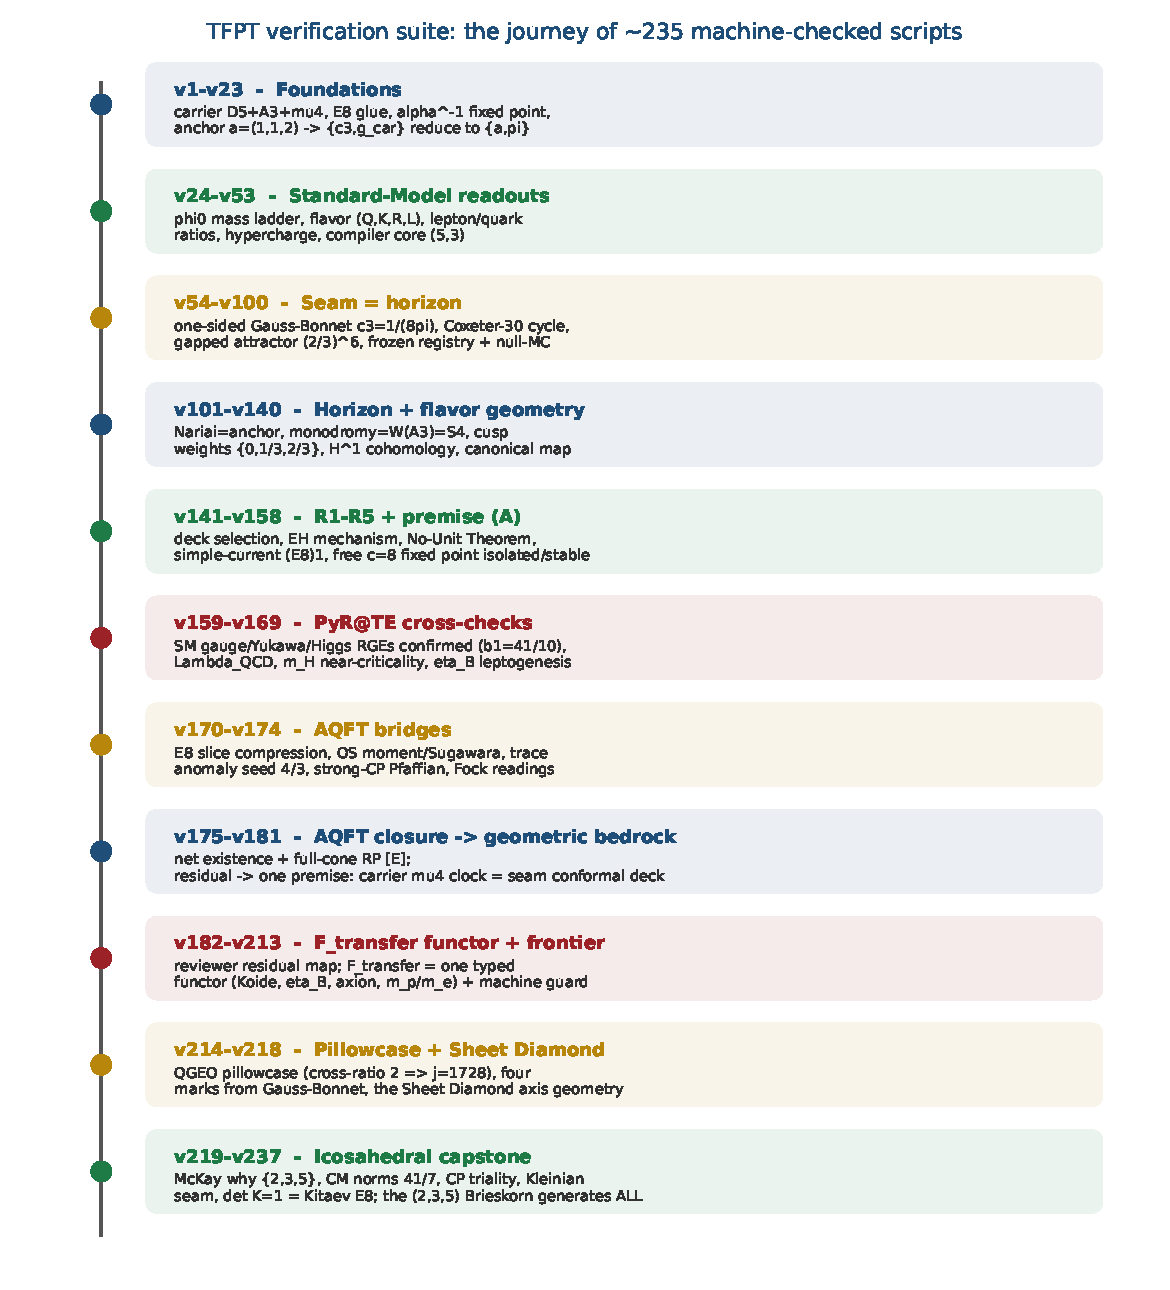
\includegraphics[width=0.96\linewidth]{figures/script_timeline.pdf}
\caption{The development timeline of the verification suite --- the eleven phases of the journey and what
each did, mathematically and physically: from the foundations (carrier, $E_8$ glue, $\alpha^{-1}$, the
anchor $a=(1,1,2)$ to which $\{\cthree,\gcar\}$ reduce) through the Standard-Model readouts, the
seam$=$horizon geometry, the horizon/flavor geometry, the R1--R5 and premise-(A) reductions, the
external PyR@TE RGE cross-checks and the AQFT bridges, the AQFT closure that drives the whole
structural residual to one geometric bedrock premise, the $F_{\mathrm{transfer}}$ functor and frontier
interfaces, the QGEO pillowcase and Sheet Diamond, to the \emph{icosahedral capstone} --- where the single
$(2,3,5)$ Brieskorn singularity is shown to generate the whole skeleton and the closing step becomes the
physical question ``is the seam short-range-entangled ($\det K=1$)?''. The master script$\to$check map follows.}
\label{fig:script-timeline}
\end{figure}

% ---------------------------------------------------------------------
%  tex-artefacts/verification.tex -- THE master script->check index.
%  The long table mapping every verification/vN_*.py to the claim it
%  machine-checks.  \input near the end of introduction.tex (inside the
%  "computational verification" appendix).
%
%  GENERATED FILE -- DO NOT EDIT BY HAND.
%  Source: verification/script_registry.csv (column what_tex).
%  Regenerate with:  python3 verification/make_script_index.py
%
%  Requires: xltabular (loaded by the including document) and the Y
%  column type (\newcolumntype{Y}{>{\raggedright\arraybackslash}X}).
% ---------------------------------------------------------------------
{\small
\renewcommand{\arraystretch}{1.25}
\begin{xltabular}{\linewidth}{@{}p{3.5cm}Y@{}}
\toprule
\textbf{Script} & \textbf{What it machine-checks} \\
\midrule
\endfirsthead
\toprule
\textbf{Script} & \textbf{What it machine-checks \emph{(continued)}} \\
\midrule
\endhead
\midrule
\multicolumn{2}{r@{}}{\scriptsize\itshape continued on next page}\\
\endfoot
\bottomrule
\endlastfoot
\texttt{v1\_\allowbreak e8\_\allowbreak glue.py} & glue theorem $E_8{=}(D_5{\oplus}A_3){+}\mu_4$: $\operatorname{disc}{=}\Z_4$, $q(D_5){+}q(A_3){=}\tfrac54{+}\tfrac34{=}2$, $240{=}16{\cdot}5{\cdot}3$, $248{=}240{+}8$ \\
\texttt{v2\_\allowbreak carrier\_\allowbreak pascal.py} & $\gcar{=}5$ unique Pascal solution; $16{=}1{+}5{+}10$, $\Nfam{=}3$, $\operatorname{rank}E_8{=}8$, $\Oadm{=}48$, $b_1{=}\tfrac{41}{10}$ \\
\texttt{v3\_\allowbreak em\_\allowbreak alpha.py} & EM closure: unique root of $F_{U(1)}(\alpha){=}0$, $\ainv{=}137.0359992168$, existence/uniqueness, inverse test, ablation \\
\texttt{v4\_\allowbreak flavor\_\allowbreak matrix.py} & residue matrix $R$: $\det{=}8$, minors $\{2,3,5\}$, $\chi_R{=}t^3{-}9t^2{+}10t{-}8$, SNF $\operatorname{diag}(1,1,8)$, $\|R\|_F^2{=}78$, $\sum L{=}40$ \\
\texttt{v5\_\allowbreak e8\_\allowbreak cascade.py} & cascade $D_n{=}60{-}2n$: endpoints, exponent rungs $\to240$, IR tail $46080$, variance $6552$ \\
\texttt{v6\_\allowbreak bootstrap.py} & reverse glue $\mu^2{-}5\mu{+}4{=}0$; $\gcar{=}5$ three ways; $8{=}\operatorname{rank}E_8{=}h(D_5){=}\varphi(30)$ \\
\texttt{v7\_\allowbreak gravity\_\allowbreak cosmo.py} & scalaron exponent $7$, $M_{\rm scal}^2/\Mbar^2{=}\cthree^7$, $A_s,n_s,r$, $\Omega_b$, $\sin^2\theta_{12}$ \\
\texttt{v8\_\allowbreak horizon.py} & horizon code: $\tfrac1{2\pi}{=}4\cthree$, $1920{=}|W(D_5)|$, $S_{dS}$, Page, $\beta_{\rm rad}{=}0.2424^\circ$ \\
\texttt{v9\_\allowbreak neutrino\_\allowbreak texture.py} & solar angle: explicit $\mu\tau$ Majorana texture $\to\sin^2\theta_{12}{=}\tfrac13{-}\tfrac{\phiz}2$, $\theta_{23}{=}45^\circ$, $\theta_{13}{=}0$ \\
\texttt{v10\_\allowbreak projection\_\allowbreak involution.py} & $Q,\Sigma$ algebra: $K{=}R{+}Q\Sigma$, $L{=}R{+}Q(I{+}\Sigma)$; $\chi_Q,\chi_K$; det ladder $3{\cdot}4{\cdot}8{\cdot}20{=}1920{=}|W(D_5)|$; $a^\top Ka{=}41$ \\
\texttt{v11\_\allowbreak unique\_\allowbreak KQ.py} & $K,Q$ are the \emph{unique} nonneg-int matrices with their compiler budgets, spectrum and monotone rows (enumeration) \\
\texttt{v12\_\allowbreak mass\_\allowbreak generation\_\allowbreak polynomials.py} & sector/generation polynomials of $K$ and the anchor-block det ladder $(9,10,16,40)$ \\
\texttt{v13\_\allowbreak open\_\allowbreak gates.py} & gate closures: $M{=}41{=}10b_1{=}\sum L{+}N_\Phi$; $Q_+$ $=$ $A_3$ exponents, $Q_-^2{=}\Nfam$ \\
\texttt{v14\_\allowbreak carrier\_\allowbreak uniqueness.py} & $\gcar{=}5$ unique ($\Nfam\in\Z^+$, rank $E_8{=}8$); split $(3,2)$ from $b{+}s{=}5,b^2{+}s^2{=}13$; $\operatorname{Tr}Y{=}\operatorname{Tr}Y^3{=}0$ \\
\texttt{v15\_\allowbreak bootstrap\_\allowbreak classification.py} & $D_5{\oplus}A_3$ unique familyful cyclic-glue of $E_8$ ($16$-spinor $+$ $3$ families), glue $\Z_4$ \\
\texttt{v16\_\allowbreak solar\_\allowbreak dual\_\allowbreak anchor.py} & $a^\top R^{-1}{=}a^\top L^{-1}{=}(-\tfrac12,-\tfrac12,1)$; $\sin^2\theta_{12}{=}\tfrac13{-}\tfrac{\phiz}{2}$; full PMNS \\
\texttt{v17\_\allowbreak hexagonal\_\allowbreak resolvent.py} & finite resolvent $D_y^{-1}{=}(\sum y^{5-m}\delta^m U_6^m)/(y^6{-}\delta^6)$ (quark $c$ backbone) \\
\texttt{v18\_\allowbreak quark\_\allowbreak yukawa.py} & quark source ratios $\tfrac{m_u}{m_d}{=}0.470085,\tfrac{m_c}{m_s}{=}13.61,\tfrac{m_t}{m_b}{=}40.80$ exact; lepton $c{=}(\tfrac{16}{7},\tfrac43,\tfrac76)$; full hierarchy \\
\texttt{v19\_\allowbreak monodromy\_\allowbreak moduli.py} & exact pole $z_\star{=}\tfrac{794-7\sqrt{9961}}{2187}$ ($3^7$); $D_4$ $SU(3)$ monodromy constructible but $D_4$-fixed locus positive-dim $\Rightarrow$ exact quark $c$ reduce to $(U)$ \\
\texttt{v20\_\allowbreak lepton\_\allowbreak c\_\allowbreak derivation.py} & lepton $c$'s derived: $\delta{=}\tfrac12$ resolvent $c{=}|\mu_4|^w/(\tfrac54{-}\cos\tfrac{r\pi}3)$ $\Rightarrow$ $\tfrac{16}7,\tfrac43$; product $\tfrac{2^{\gcar}}{\Nfam^2}{=}\tfrac{32}9$ $\Rightarrow$ $\tfrac76$ \\
\texttt{v21\_\allowbreak solar\_\allowbreak product\_\allowbreak quark.py} & solar coeff $=q(A_3){=}\tfrac34$ (glue-norm, $q(D_5){+}q(A_3){=}2$), $\sin^2\theta_{12}{=}\tfrac13{-}\tfrac{\phiz}2$; product $\tfrac{2^{\gcar}}{\Nfam^2}$; quark law fails ($\tfrac17$ vs $0.724$) \\
\texttt{v22\_\allowbreak open\_\allowbreak gates\_\allowbreak audit.py} & residual-gates audit contract: exact reduction of each open gate (A2,B3,B4,B5,B6,C7) machine-pinned (forced part vs.\ named residual) \\
\texttt{v23\_\allowbreak anchor\_\allowbreak generator.py} & anchor $a{=}(1,1,2)$: $e_k{=}(4,5,2)$, $\cthree{=}\tfrac1{2e_1\pi}$; $p_n{=}2{+}2^n\!\Rightarrow\!240,248$, binary ladder; inputs $\to\{a,\pi\}$ \\
\texttt{v24\_\allowbreak quark\_\allowbreak ratio\_\allowbreak closure.py} & quark ratios $\tfrac{55}{117},\tfrac{34}{47},\tfrac3{26}$ from TFPT blocks; mass ratios match $<0.03\%$; rational $c$ gauge, $\Lambda_q$ in $O(1)$ \\
\texttt{v25\_\allowbreak frontier\_\allowbreak conjectures.py} & conjectures: Koide $Q_{\mathrm{src}}{+}\tfrac{\phiz}{24}{\approx}\tfrac23$; axion $f_a{=}M_{\mathrm{scal}}/128{\to}m_a{\approx}23.8\,\mu$eV \\
\texttt{v26\_\allowbreak flavor\_\allowbreak frontier\_\allowbreak unification.py} & the ``$11$'' is not uniquely forced ($\Rightarrow$\,\mC); flavor frontier unifies to one $(U)$ gate; cusp config on the parabolic stability wall \\
\texttt{v27\_\allowbreak wall\_\allowbreak representative.py} & explicit balanced wall rep $W_{\mathrm{wall}}$ (cols $=$ perm$(0,1,2)$, rows $w{=}(2,1,1)$, pardeg $0$); selector $\det R{=}8$, $\mathrm{Spec}(Q_+){=}\{1,2,3\}$ \\
\texttt{v28\_\allowbreak gravity\_\allowbreak fR.py} & $R{+}R^2$ closed: $f(R)$, $M{=}\cthree^{7/2}\Mbar$ scalaron, $N_\star{=}57\!\to\!n_s,r,A_s$; full metric measure open; $248\cthree^2{<}6\log\tfrac32$ \\
\texttt{v29\_\allowbreak research\_\allowbreak contract\_\allowbreak certs.py} & research-contract certificates: $C_U^{(1)}$ wall enumeration ($1296{\to}144{\to}5$ orbits; symmetry alone does not pick $W_{\mathrm{wall}}$) and $G5$ gap-dominance $2\|V\|{<}\Delta$ \\
\texttt{v30\_\allowbreak d4\_\allowbreak character\_\allowbreak variety.py} & $C_U^{(2)}$: full $D_4$-fixed $SU(3)$ character variety is positive-dimensional $\Rightarrow$ selector needs the $R(\rho)$ dictionary (H2; exact since \vref{v118}--\vref{v122}, residue $=$ the R4$'$ selector establishment) \\
\texttt{v31\_\allowbreak R\_\allowbreak dictionary.py} & $R(\rho)$ characterized: case A alive (irreducible $\Rightarrow$ mixing); $R$ integer but $\rho$-invariants continuous $\Rightarrow$ $R(\rho)$ is the transcendental non-abelian-Hodge map (residual $=$ Hitchin solve) \\
\texttt{v32\_\allowbreak rh\_\allowbreak splitting.py} & RH route: $\sum_kU^kA_0U^{-k}{=}4\operatorname{diag}(A_0)$ exact $\Rightarrow$ splitting $\mathcal O(-2){\oplus}\mathcal O(-1)^2\!\Leftrightarrow\!\operatorname{diag}(A_0){=}(\tfrac12,\tfrac14,\tfrac14)$ (algebraic); $\prod M_k{=}I$ + $R$-bridge stay open ($c_u/c_d$ not forced) \\
\texttt{v33\_\allowbreak explicit\_\allowbreak flat\_\allowbreak bundle.py} & explicit valid $(U_{\mathrm{wall}})$ flat bundle (RH solve): cusp $+$ $\mathcal O(-2){\oplus}\mathcal O(-1)^2$ $+$ $\|M_\infty{-}I\|{\sim}10^{-9}$ ($\prod M_k{=}I$) $+$ irreducible (case A) \\
\texttt{v34\_\allowbreak h2\_\allowbreak bridge\_\allowbreak attempt.py} & H2 bridge: explicit per-puncture $M_k$ (cusp, $\prod M_k{=}I$); honest negative --- natural extraction $\neq$ lepton amplitudes, the $\Gamma^{\min}$ dictionary is the remaining input ($c_u/c_d$ not obtained) \\
\texttt{v35\_\allowbreak quark\_\allowbreak qcd\_\allowbreak boundary.py} & the open gates are the discrete$\leftrightarrow$continuous boundary: quark cross-ratio cleanness tracks generation/QCD sensitivity (compiler hands off to continuous physics) \\
\texttt{v36\_\allowbreak spectral\_\allowbreak action\_\allowbreak g2.py} & G2: spectral action $\to R{+}R^2$ ($a_2{\sim}{-}R/3$, $a_4|_{R^2}{\sim}R^2/72$); $M^2/\Mbar^2{=}6(4\pi)^2/f_0$, $\cthree^7$ fixes $f_0$; gap-decoupling $\Delta_{\mathrm{eff}}{=}1.648{>}0\Rightarrow$ admissible IR closed under RP, ambient (G6) $=$ strict-TOE completion target \\
\texttt{v37\_\allowbreak plucker\_\allowbreak anchor.py} & anchor-plane Plücker apparatus: $\|\mathrm{Pl}(K)\|_1{=}11$, $\|\mathrm{Pl}_R(K)\|_1{=}26$, $\sum\mathrm{Pl}_R(L){=}60$; pencil $\det(K{+}xQ){=}3x^3{+}7x^2{+}6x{+}4$; $K_e{-}K_u{=}a$, $L_e{-}L_u{=}\mathrm{Exp}(A_3)$; lepton ring $c_ec_\tau{=}|\Z_2|c_\mu$; Koide $u{\to}\tfrac{53}{54}u$ (\mC) \\
\texttt{v38\_\allowbreak uwall\_\allowbreak killswitch.py} & $(U_{\mathrm{wall}})$ U2 kill-switch hardened: $D_4$-cusp rep irreducible at all $400$ sampled points (commutant${=}1$), mixing ${\ge}0.35$, reducible locus measure-zero $\Rightarrow$ case A generic, $(U_{\mathrm{wall}})$ survives; amplitude dictionary still research-level \\
\texttt{v39\_\allowbreak uwall\_\allowbreak selectors.py} & $(U_{\mathrm{wall}})$ selector side closed on the explicit point: splitting type ${=}$ anchor $a{=}(1,1,2)$, pardeg ${=}0$; $\det R{=}8{=}n{\cdot}a$, $\mathrm{Spec}(Q_+){=}\{1,2,3\}{=}3\alpha{+}1$ read off the bundle; only the amplitudes $c_u/c_d$ ($\Gamma^{\min}$ Hitchin) remain \\
\texttt{v40\_\allowbreak harmonic\_\allowbreak metric.py} & $(U_{\mathrm{wall}})$ harmonic metric ${=}$ FINITE linear algebra (polystable${\Rightarrow}$unitary${\Rightarrow}\Phi{=}0$): unique invariant form $H{>}0$, unitarised $\widetilde M_k$ cusp-class with $|\widetilde M_k|{\in}\{0,\tfrac12,\tfrac1{\sqrt2}\}$; the feared Hitchin PDE collapses to unitarisation $+$ combinatorial $R$ \\
\texttt{v41\_\allowbreak leg\_\allowbreak assignment.py} & $(U_{\mathrm{wall}})$ final leg test: amplitudes ${=}$ $\delta{=}\tfrac12$ resolvent (closed); $\Lambda_\mu{>}1$ rules out holonomy moduli; harmonic holonomy $|\mathrm{diag}|{=}(0,\tfrac12,\tfrac12)$ supplies $\delta{=}\tfrac12$ (suggestive); honest negative on literal $c_u/c_d$ reproduction \\
\texttt{v42\_\allowbreak exterior\_\allowbreak leg.py} & $(U_{\mathrm{wall}})$ Exterior Leg Lemma: $u,d$ share $(r,w){=}(1,1)$ so any scalar leg gives $c_u/c_d{\equiv}1$; the $u/d$ split is the $\Lambda^2F$ area $\mathrm{Pl}_{\mathbf1,a}(K)$, $\|{\cdot}\|_1{=}11$ generated $\Rightarrow$ $\tfrac{5\cdot11}{9\cdot13}{=}\tfrac{55}{117}$ \mE; phys.\ identification \mC\ \\
\texttt{v43\_\allowbreak exterior\_\allowbreak bridge.py} & $(U_{\mathrm{wall}})$ $\Lambda^2F$ bridge: $\Lambda^2(\widetilde M){=}\overline{\widetilde M}$ (exterior leg ${=}\mathbf{\bar3}$) confirmed; continuous action $\neq$ integer $\mathrm{Pl}(K)$ $\Rightarrow$ bridge is the discrete H2 invariant ($\det R{=}8$, $\mathrm{Spec}(Q_+)$ confirmed), not continuous \\
\texttt{v44\_\allowbreak carrier\_\allowbreak exterior.py} & $(U_{\mathrm{wall}})$ Lie-level grounding: $16{=}\Lambda^{\mathrm{even}}(5){=}1{+}10{+}5$; $u^c{\in}\Lambda^2(5)$, $d^c{\in}\Lambda^4(5)$ $\Rightarrow$ exterior degrees $(2,4)$, sum${=}6{=}|R^+\!(A_3)|$, diff${=}2{=}|\Z_2|$; the exterior leg is the carrier's own $\Lambda^2$ grading (no special math) \\
\texttt{v45\_\allowbreak family\_\allowbreak exterior.py} & $(U_{\mathrm{wall}})$ the ``$11$'' is Pascal: $|\mathrm{Pl}(K)|{=}(1,4,6){=}\{\Lambda^0,\Lambda^1,\Lambda^2\}(\mu_4)$; $\|\mathrm{Pl}(K)\|_1{=}11{=}\sum_{k\le2}\binom4k{=}16{-}\gcar$ (cumulative ext of $\mu_4$ up to $\deg u^c{=}2$); $15{=}\dim\mathfrak{su}(4){=}10{+}5{=}\Nfam\gcar$ \\
\texttt{v46\_\allowbreak grand\_\allowbreak mass\_\allowbreak volume.py} & absolute mass-scaling is \mE, not a product rule: sector dets $(\phiz)^{6},(\phiz)^{9},(\phiz)^{10}$ (exponents $|R^+\!A_3|,\Nfam^2,\mathcal A_\Lambda$) $\Rightarrow$ $\det M_{\mathrm{SM}}{\sim}(\phiz)^{25}{=}(\phiz)^{\gcar^2}$; $Q$-rows $(4,5,6)$ sum $15{=}\dim A_3$; $25{+}15{=}40{=}\sum L$ \\
\texttt{v47\_\allowbreak selection\_\allowbreak theorem.py} & Boundary Carrier Selection (Thm A): $\mu_4{\to}A_3,\Nfam{=}3$; $16$-spinor${\to}D_5$; $q(D_5){+}q(A_3){=}2$, glue $4{=}|\mu_4|$; only $D_5{\oplus}A_3$ meets all four conditions ($D_8,E_7{+}A_1,E_6{+}A_2,A_4{+}A_4,A_8$ excluded) \mE/\mC \\
\texttt{v48\_\allowbreak em\_\allowbreak ward.py} & EM boundary Ward (Thm C): $F_{U(1)}{=}$ Maxwell $\alpha^3$ $-$ Calder\'on $2\cthree^3\alpha^2$ $-$ transport $8b_1\cthree^6\log\tfrac1{\varphi_{\mathrm{seam}}}$; $8b_1{=}\tfrac45 M{=}\tfrac{164}5$, $-\tfrac54{=}q(D_5)$ \mE; Ward origin \mC \\
\texttt{v49\_\allowbreak readout\_\allowbreak rigidity.py} & Readout Rigidity (Thm U2): $c_u/c_d{=}\tfrac{55}{117}$ is constant on the discrete selector stratum $\mathcal S_{8,Q}$ $\Rightarrow$ no point-uniqueness needed; $(U_{\mathrm{wall}}){=}U_{\mathrm{unitary}}{+}U_{\mathrm{H2}}{+}U_{\Lambda^2}{+}U_{\mathrm{point}}$, only $U_{\mathrm{point}}$ open \\
\texttt{v50\_\allowbreak q\_\allowbreak geometry.py} & Q geometry (Thm Q): $Q_+{=}$ diag$(3,2,1)$-block $\chi{=}(t{-}1)(t{-}2)(t{-}3)$, $Q_-$ $\chi{=}t(t^2{-}3)$; $Q$ unique under rows$(4,5,6)$/cols$(9,5,1)$/spectra; geom.\ origin \mC \\
\texttt{v51\_\allowbreak boundary\_\allowbreak half\_\allowbreak step.py} & glue norms ${=}(\gcar,\Nfam)/|\mu_4|$: $q(D_5){=}\tfrac54$, $q(A_3){=}\tfrac34$; four ops forced ${\to}$ $\{$sum$=2$ root norm, diff$=\tfrac12{=}|\Z_2|/|\mu_4|{=}\delta$, prod$=\tfrac{15}{16}$, ratio$=\tfrac53\}$. So $\delta{=}\tfrac12$ is the carrier$-$family count over the glue index, not chosen \mE \\
\texttt{v52\_\allowbreak pencil\_\allowbreak endpoints.py} & $K{+}xQ$ pencil endpoints: $P({-}1){=}2{=}|\Z_2|$, $P(0){=}4{=}|\mu_4|$, $P(1){=}20{=}\det L$, $P(2){=}68{=}2p_5(a)$; $\det(K{-}Q){=}2$, $\operatorname{tr}{=}\Nfam$ (audit ext.\ of \vref{v37}) \mE \\
\texttt{v53\_\allowbreak compiler\_\allowbreak core.py} & Big picture: the whole integer skeleton from $(\gcar,\Nfam){=}(5,3)$ --- $\operatorname{rank}E_8{=}8$, $|\Z_2|{=}2$, Pythagorean $\Delta_Y{=}\gcar^2{=}25{=}\Nfam^2{+}|\Z_2|\!\cdot\!\operatorname{rank}E_8{=}9{+}16{=}\dim S^+$ (diff.\ of squares); anchor char-poly $(t{-}1)^2(t{-}2)$ unique \mE \\
\texttt{v54\_\allowbreak seam\_\allowbreak horizon\_\allowbreak keystones.py} & The ``$8$'' in $\cthree{=}\tfrac1{8\pi}$ overdetermined and gravitationally aligned ($2|\mu_4|{=}\operatorname{rank}E_8{=}h(D_5){=}\varphi(30){=}8\pi$ Hawking/Einstein); one boundary transport operator (spec $\{1,(2/3)^6,(1/3)^6\}$, $\lambda_2{=}(2/3)^6$) governs \emph{both} SM flavor gap and horizon Page recovery \mE \\
\texttt{v55\_\allowbreak coxeter\_\allowbreak cycle.py} & Computed $E_8$ Coxeter element: order exactly $30{=}|\Z_2|\Nfam\gcar$, eigenphases ${=}$ exponents ${=}$ totatives of $30$, so $\operatorname{rank}E_8{=}8{=}\varphi(30){=}$ live phases of the order-$30$ cycle; one $\alpha^{-1}$ sets EM, $S_{dS}$ and $\Lambda$ ($S_{dS}\rho_\Lambda{=}32\pi^4$) \mE \\
\texttt{v56\_\allowbreak unique\_\allowbreak attractor.py} & Gapped boundary transport (gap $6\log\tfrac32{>}0$) $\Rightarrow$ \emph{unique} attracting fixed point, geometric rate $(2/3)^6$ (two starts $\to$ same direction); Coxeter in $|\mu_4|{=}4$ planes; entropy reset ${=}$ rank-$1$ projector \mE \\
\texttt{v57\_\allowbreak horizon\_\allowbreak crosslinks.py} & Horizon cross-links: $\cthree{=}\tfrac1{8\pi}$ is the Einstein/Jacobson coefficient ($1/4{=}1/|\mu_4|$ entropy density); Hod QNM $\omega_R/T_H{=}\ln3{=}\ln\Nfam$; Hawking power denom $1920{=}|W(D_5)|$; one $\alpha^{-1}$ for EM/$S_{dS}$/$\Lambda$/Hubble \mE\ (+ \mC\ identification) \\
\texttt{v58\_\allowbreak seam\_\allowbreak horizon\_\allowbreak chain.py} & Seam-horizon chain (precise: seam $=$ abstract normaliser, locally realised as a horizon): one-sided $S^2$ Gauss--Bonnet $\cthree{=}1/(2{\cdot}4\pi){=}\tfrac1{8\pi}$; KMS $4\cthree\kappa$; $S_{BH}{=}M^2/2\cthree$; RT in seam units. Seam--Horizon Theorem (area-law from the seam kernel) \mO\ open \\
\texttt{v59\_\allowbreak area\_\allowbreak law\_\allowbreak evidence.py} & Area-law necessary condition met: a reflection-positive Gaussian (Calder\'on-type) kernel yields an area law (gapped block-EE saturates; gapless $\sim\tfrac c3\log L$), by the \emph{same} gap that fixes the attractor; $8{=}|\Z_2||\mu_4|$. The $\cthree$ coefficient stays \mO\ open \\
\texttt{v60\_\allowbreak lambda\_\allowbreak metrology\_\allowbreak branch.py} & $\Lambda$ branch selection: $(8\pi)^2\delta_{\mathrm{top}}{=}\tfrac3{4\pi^2}$, mis-scale $2\cthree/\delta_{\mathrm{top}}{=}\tfrac{64\pi^3}3{=}661.47$ $\Rightarrow$ $G_N$ pinned as output; $123$ orders $=119.028{+}3.920$; ACT DR6 birefringence $0.215^\circ{\pm}0.074^\circ$ vs $0.2424^\circ$ ($0.37\sigma$) \mE \\
\texttt{v61\_\allowbreak cft\_\allowbreak bridge.py} & Boundary-CFT mirror: level-$1$ WZW central charges $c(E_8){=}8$, $c(D_5){=}5$, $c(A_3){=}3$ $=$ $(\operatorname{rank}E_8,\gcar,\Nfam)$; conformal embedding $c_{\mathrm{coset}}{=}0$; $SU(3)\!\leftrightarrow\!SU(4)$ reconciliation $\Nfam{=}|\mu_4|{-}1$, $4{\to}3{+}1$ (one geometry $\mathbb P^1\!\setminus\!\mu_4$, two sides) \mE \\
\texttt{v62\_\allowbreak data\_\allowbreak scorecard.py} & TFPT vs 2024/25 data: $\alpha^{-1}$, $\sin^2\theta_{12}$, $\beta_{\mathrm{rad}}$ match; $\sin^2\theta_{13}$ ($2.0\sigma$) and Starobinsky $n_s$ vs DESI ($\sim2\sigma$) mild tensions; $\theta_{23}$ open; $r{\approx}0.004$ future falsifier \mE \\
\texttt{v63\_\allowbreak seam\_\allowbreak engineering\_\allowbreak index.py} & Exact Seam-Engineering Index $\Xi{=}2\|V\|/\Delta{=}\tfrac{31}{24\pi^2\log(3/2)}{\approx}0.323$ ($2\|V\|{=}\tfrac{31}{4\pi^2}$, $248{=}\dim E_8$, $31{=}1{+}h^\vee$), $\Delta_{\mathrm{eff}}{\approx}1.648$; four-class possibility taxonomy \mE/\mO \\
\texttt{v64\_\allowbreak causal\_\allowbreak boundary\_\allowbreak nogo.py} & Causal Boundary Engineering \emph{conditional no-go}: gapped transfer has no periodic orbit (discrete no-CTC); RP$+$OS$+$gap $\Rightarrow$ ANEC $\Rightarrow$ Topological Censorship $\Rightarrow$ no traversable shortcut; only ER$=$EPR bridge survives \mE\,(core)/\mC\,(chain) \\
\texttt{v65\_\allowbreak falsification\_\allowbreak layer.py} & Prediction layer with explicit failure thresholds: 3 core ($v_{\mathrm{GW}}{=}c$, no 4th gen, seam${=}8$), 4 observational ($\beta$, $r$, $n_s$, $\theta_{12}$), no-go $+$ unitarity; $N_\star$ demoted to \mC\ input; none violated \mE \\
\texttt{v66\_\allowbreak e8\_\allowbreak casimir\_\allowbreak degrees.py} & Organizing simplification: the compiler atoms \emph{are} the $E_8$ Casimir degrees $\{2,8,12,14,18,20,24,30\}$ ($2{=}|\Z_2|$, $8{=}\operatorname{rank}$, $14{=}\dim G_2$, $20{=}\det L$, $24{=}|W(A_3)|$, $30{=}h(E_8)$); $\sum{=}128{=}2^7$ (dS prefactor), $\sum\text{exp}{=}120{=}|R^+(E_8)|$ \mE \\
\texttt{v67\_\allowbreak area\_\allowbreak law\_\allowbreak coefficient.py} & Central-theorem \emph{structural closure}: Fursaev--Solodukhin $S{=}4\pi k A$, $k{=}\cthree/2$ $\Rightarrow$ $S{=}2\pi\cthree A{=}\tfrac14 A$ ($2\pi\cthree{=}\tfrac14$); $\cthree{=}\tfrac1{8\pi}$ is the \emph{unique} value with replica-coeff ${=}$ BH $\tfrac14$. Reduces to the one coeff $k{=}\cthree/2$ (then \emph{forced}, \vref{v73}) \mE \\
\texttt{v68\_\allowbreak seeley\_\allowbreak dewitt\_\allowbreak residual.py} & Residual \emph{resolved as an anchor}: $a_2{=}{-}\tfrac{d}{192\pi^2}R$ $\Rightarrow$ the \emph{absolute} $\tfrac1{16\pi G}$ is UV-sensitive ($\propto d\Lambda^2 f_2$), so the \emph{scale} $1/G$ is the one dimensionful anchor (the dimensionless $k{=}\cthree/2$ is forced, \vref{v73}); cutoff-indep.\ $R^2$/scalaron derived \mE \\
\texttt{v69\_\allowbreak d4\_\allowbreak q\_\allowbreak geometry.py} & $D_4$-equivariant Q-geometry (gate \mC/\mE): on $H_1(\PP^1\!\setminus\!\mu_4){=}B_1{\oplus}E$, $Q_+{=}3w{+}1{=}\operatorname{diag}(1,2,3)$ (cusp weights on $\mu_4{=}\Z_4$ eigenspaces), $Q_-{=}E$-coupling $\sqrt{\Nfam}$ $\Rightarrow$ $t(t^2{-}3)$; $\Sigma$-split ${=}D_4{=}\Z_4{\rtimes}\Z_2$ \mE \\
\texttt{v70\_\allowbreak q\_\allowbreak integer\_\allowbreak lift.py} & Q integer-lift sharpened: $\Z_4$ puncture action $R$ unimodular (eigenvalues $\{-1,i,-i\}$); $\det Q{=}3{=}\Nfam$, SNF $\operatorname{diag}(1,1,3)$ $\Rightarrow$ residual ${=}$ one lattice invariant $\det Q{=}\Nfam$, not closable by $D_4$ alone \mE \\
\texttt{v71\_\allowbreak simple\_\allowbreak r\_\allowbreak bridge.py} & \emph{Simple} R-bridge (gate \#3): selector stratum $\mathcal S_{8,Q}$ now fully derived ($\det R{=}8{=}\operatorname{rank}E_8$ lattice $+$ $\operatorname{Spec}(Q_+){=}\{1,2,3\}$ from \vref{v69}) $\Rightarrow$ quark \emph{ratios} are pure integer Pl\"ucker readouts ($\tfrac{55}{117}$, no monodromy, \vref{v49} rigidity); residual $U_{\mathrm{point}}{=}$ absolute norm.\ $=$ an anchor \mE/\mO \\
\texttt{v72\_\allowbreak q\_\allowbreak det\_\allowbreak from\_\allowbreak cusp.py} & $\det Q{=}\Nfam$ derived from the cusp class: $\det Q{=}|\!\operatorname{coker}Q|{=}$ cusp-class order $=$ denominator of the weights $\{0,\tfrac13,\tfrac23\}$ (same data as $\operatorname{Spec}Q_+$); $\operatorname{coker}Q{=}\Z/\Nfam{=}$ triality deck group $\Rightarrow$ integer-lift residual closed \mE \\
\texttt{v73\_\allowbreak k\_\allowbreak c3\_\allowbreak half.py} & Central coefficient $k{=}\cthree/2$ \emph{forced}: $(1/2)$ variational $\times$ $1/(|\Z_2|2\pi\chi(S^2))$ Gauss--Bonnet topology ($\chi(S^2){=}2$), both cutoff-indep $\Rightarrow$ Fursaev--Solodukhin $S{=}A/4$; only the absolute $4$D Newton scale stays the anchor (\vref{v68}) \mE \\
\texttt{v74\_\allowbreak compiler\_\allowbreak micro\_\allowbreak lemmas.py} & Spine quotient ladder ($\tfrac23,\tfrac34,\tfrac45,\tfrac54,\tfrac43$ $=$ adjacent quotients of $(2,3,4,5)$); pencil differences $(2,16,48){=}(|\Z_2|,\dim S^+,\Oadm)$ sheet$\to$1gen$\to$3gens; anchor QF $a^\top K a{-}\mathbf1^\top K\mathbf1{=}41{-}25{=}16{=}\dim S^+$ (EM budget $=$ mass vol $+$ one gen); solar dual anchor $L{=}R{+}6\mathbf1 e_1^\top$, $a^\top R^{-1}\mathbf1{=}0$ (Sherman--Morrison rank-one invariance) \mE \\
\texttt{v75\_\allowbreak upoint\_\allowbreak to\_\allowbreak vgeo.py} & \textbf{Gate 1 complete:} $U_{\mathrm{point}}{\to}v_{\mathrm{geo}}$. Ratios closed (\vref{v49}/\vref{v71}) $+$ lepton $c$ exact (\vref{v20}) $+$ sector products $=\phiz$-powers (\vref{v46}); $(\text{ratios},\text{product}){\Leftrightarrow}(\text{individuals})$ bijection $\Rightarrow$ absolute amplitudes fixed up to \emph{one} scale $v_{\mathrm{geo}}$ $=$ the same anchor as $1/G$ (\vref{v68}); two $[A]\to$ one \mE/\mO \\
\texttt{v76\_\allowbreak gmetric\_\allowbreak reduction.py} & \textbf{Gate 2:} Tier A (IR) closed under RP$+$gap (Decoupling Thm: $\Delta_{\mathrm{eff}}{=}6\log\tfrac32{-}\tfrac{31}{4\pi^2}{=}1.648{>}0$, $\|V\|{\le}248\cthree^2{=}\tfrac{31}{8\pi^2}$); Tier B (strict TOE) holographically reduced from bulk to a finite seam-\emph{boundary} measure (conditional: RP$+$tightness $\Rightarrow$ closes) \mE/\mC \\
\texttt{v77\_\allowbreak e8\_\allowbreak conformal\_\allowbreak net.py} & \textbf{G6 route:} the seam boundary measure $=$ the $(E_8)_1$ \emph{lattice net} (rigorous, holomorphic $c{=}8$); level-1 $c(E_8){=}\tfrac{248}{31}{=}8$, $c(D_5){=}5$, $c(A_3){=}3$, embedding $5{+}3{=}8$ (coset $c{=}0$); imports $G6$ into RCFT/conformal-net rigor \mE/\mC \\
\texttt{v78\_\allowbreak vgeo\_\allowbreak floor.py} & \textbf{$v_{\mathrm{geo}}$ floor:} no pure number is dimensionful $\Rightarrow$ $v_{\mathrm{geo}}$ irreducible by logic; all scales are ratios $\times$ one $\bar M_{\mathrm{Pl}}$; $S_{dS}\rho_\Lambda{=}32\pi^4$ pins it from one measurement; theory at the minimum (one scale $+$ $\pi$) \mE/\mO \\
\texttt{v79\_\allowbreak review\_\allowbreak identities.py} & Four validated review identities $+$ one firewall: hypercharge Lucas--Binet $D_n{=}(3^n{-}(-2)^n)/5{=}1,1,7,13,55,133$ (roots $=$ carrier charges); Inverse Anchor Thm ($\mathbf1^\top M^{-1}\mathbf1{=}1/$atom, $a^\top M^{-1}a{=}1$ for $R,K,L$); MacWilliams $(1,10,5)$; $6Y^2{-}Y{-}1{=}(2Y{-}1)(3Y{+}1)$. Rejects $m_p/m_e$, $\eta_B$ near-formulas (firewall) \mE \\
\texttt{v80\_\allowbreak operator\_\allowbreak pencil\_\allowbreak geometry.py} & Operator-pencil geometry: Anchor Singularity Thm $\det B_{K+xQ}{=}(\Nfam x{+}|\Z_2|)(\Nfam x{+}\gcar){=}(3x{+}2)(3x{+}5)$ ($\tfrac23$ Koide/gap $=$ anchor-plane singularity); buildup chain $(3,10,16,20)$; type checker $\det B_{Q,K,R,L}{=}(9,10,16,40)$; audit: differential spectrum, $F_4{\times}G_2$ shadow $248{=}52{+}14{+}26{\cdot}7$ \mE/\mC \\
\texttt{v81\_\allowbreak singular\_\allowbreak pencil\_\allowbreak matrices.py} & Double cover $y^2{=}\det B_{K+xQ}{=}(3x{+}2)(3x{+}5)$: Koide $x{=}{-}\tfrac23$ and carrier $x{=}{-}\tfrac53$ are the two branch points (deck $2{=}|\Z_2|$; disc${=}81{=}\Nfam^4$; separation${=}1$ transport period). Clearing matrices $C_{2/3}{=}3K{-}2Q$ ($D_5{\oplus}A_3$ glue, $B{=}(5,7)^\top(9,11)$, $\sum{=}240$), $C_{5/3}{=}3K{-}5Q$ (neutral, $\chi{=}(\lambda{+}2)(\lambda^2{+}\lambda{+}6)$); scalaron $7{=}$ mixed anchor disc$/\Nfam$ \mE \\
\texttt{v82\_\allowbreak koide\_\allowbreak attractor\_\allowbreak splitting.py} & Koide attractor \emph{forced}: the branch-divisor-preserving M\"obius map fixing $q{=}2,5$ is unique, multiplier $(2/3)^6{=}\lambda_2$ of the established transfer operator $\Rightarrow$ $F'(2){<}1$ attractor, $F'(5){>}1$ repeller; three postulates $\to$ one \mC. Splitting trichotomy disc $81/49/40$: the clean split is non-generic (anchor-first) \mE/\mC \\
\texttt{v83\_\allowbreak e8net\_\allowbreak holomorphic\_\allowbreak uniqueness.py} & Holomorphy pins $(E_8)_1$: \#primaries ${=}\det$ Cartan ($D_8{:}4$ vs $E_8{:}1$), and a holomorphic $c{=}8$ chiral CFT is the lattice theory of the \emph{unique} even unimodular rank-$8$ lattice (Minkowski--Siegel mass $1/|W(E_8)|$); carrier Pascal truncation $K{=}(g{-}1)/2$ $=$ half-spinor split \mE \\
\texttt{v84\_\allowbreak frozen\_\allowbreak registry.py} & Blind-prediction registry frozen 2026-06-09 (25 digits, machine-enforced lock formula$\leftrightarrow$value): exactly \emph{one} $\theta_{12}$ prediction of record; $r$, $n_s$ as $N_\star$ \emph{bands}; conditional entries carry their hypothesis by name \mE \\
\texttt{v85\_\allowbreak master\_\allowbreak cover.py} & Master-cover theorem: $\det B$ is $\mathrm{GL}(2)$-covariant on $\operatorname{span}\{K,Q\}$ $\Rightarrow$ exactly \emph{one} double cover up to M\"obius (disc $=\Nfam^4\det(G)^2$); the disc-$81$ family is its orbit ($-\tfrac83{=}{-}\mathrm{rank}E_8/\Nfam$ $=$ carrier $-$ one period); $\mu_4$ is \emph{not} a $4{:}1$ cover (ladder of double covers); branch trace fixes only the scalaron \emph{scale} \mE \\
\texttt{v86\_\allowbreak nstar\_\allowbreak reheating.py} & $N_\star$ band $\to$ point \mC: $\Gamma{=}4M^3\!/48\pi\bar M^2{=}128$\,GeV, $T_{\mathrm{reh}}{=}9.6{\times}10^9$\,GeV, $N_\star(0.05/\mathrm{Mpc}){=}51.4$ $\Rightarrow$ $n_s{=}0.9611$, $r{=}0.0045$ (inside the frozen band); honest tensions: $n_s$ $+0.9\sigma$, $A_s$ dichotomy (slow point $-11.4\sigma$ $\Rightarrow$ near-instant reheating or exponent fails) \mC \\
\texttt{v87\_\allowbreak bulk\_\allowbreak uniqueness\_\allowbreak reduction.py} & Red-team Target A residual (ii) conditionally closed: holomorphic $\Rightarrow$ Rep $=$ Vect $\Rightarrow$ 2D bulk \emph{unique} (LR/KLM/BKLR); machine contrast $SO(16)_1$ admits \emph{six} modular invariants (incl.\ both $E_8$ pairings) $\Rightarrow$ Target A $=$ one residual \mE/\mC/\mO \\
\texttt{v88\_\allowbreak cp\_\allowbreak phase\_\allowbreak audit.py} & Target-D CP residual quantified: frozen $\delta{=}\pi/3{+}3\lambda^2$ survives at $+0.98\sigma$ vs $\gamma_{\mathrm{PDG}}$; the $0.07^\circ$-near alternative $\pi/3{+}2\lambda^2$ recorded as look-elsewhere trap, \emph{not} adopted; decision at $\sigma_\gamma{\le}0.96^\circ$ \mE \\
\texttt{v89\_\allowbreak carrier\_\allowbreak index\_\allowbreak lemma.py} & Carrier Index Lemma: KLM $\mu_A{=}[B{:}A]^2\mu_B$ $\Rightarrow$ Jones index $[(E_8)_1{:}(D_5)_1{\times}(A_3)_1]{=}4{=}|\mu_4|$ (glue order \emph{is} the index); $\mu$-additivity $16/4^2{=}1$ $\Rightarrow$ holomorphy \emph{follows}; Gate A (H)$\Leftrightarrow$(H$'$) index-$4$ extension \mE \\
\texttt{v90\_\allowbreak conical\_\allowbreak defect\_\allowbreak chain.py} & Fursaev--Solodukhin factor $4\pi$ \emph{derived} (smoothed-cone Gauss--Bonnet, exactly smoothing-independent); replica $S{=}4\pi kA$, $k{=}\cthree/2$ $\Rightarrow$ $S{=}A/4\Leftrightarrow\cthree{=}\tfrac1{8\pi}$ (sympy-solved); residual isolated to ``seam determinant $\Rightarrow$ EH form'' \mE/\mO \\
\texttt{v91\_\allowbreak spine\_\allowbreak tetrahedron.py} & Spine tetrahedron $\{2,3,4,5\}$ $=$ anchor $+$ zeroth moment; edges/faces/volume $=$ the integer grammar, volume $120{=}|R^+(E_8)|$; $240{=}|\mu_4||E(K_4)||E(K_5)|$ with $K_6$ negative control; dual cuts typed tautological; sub-grammar incompleteness honest \mE \\
\texttt{v92\_\allowbreak glue\_\allowbreak uniqueness.py} & Glue uniqueness: of all $15$ subgroups of the discriminant form exactly two Lagrangian glues (the two \emph{chiralities}, swapped by either single spinor conjugation, fixed by the simultaneous one) and exactly one halfway extension $=SO(16)_1$; tower carrier${\to}SO(16)_1{\to}(E_8)_1$, nothing else \mE \\
\texttt{v93\_\allowbreak koide\_\allowbreak relaxation\_\allowbreak toy.py} & Koide relaxation toy (P2 narrowed): basin lemma (every physical configuration in the attractor basin); exact rate $(2/3)^6$; source at $\rho{=}{-}\phiz/24$ to $0.8\%$ (\mC); honest negatives: flow time $t{=}2.84\notin\Z$ $\Rightarrow$ the missing object is a \emph{continuous} generator \mE/\mC \\
\texttt{v94\_\allowbreak sheet\_\allowbreak diamond.py} & Sheet diamond: all four flavor operators on \emph{one} surface $M(s,t){=}R{+}Q\operatorname{diag}(s,t,t)$ (pencil $=$ the cut $(1{+}x,x{-}1)$; diagonal-cut disc $153$ negative control); winding line $\det B{=}2\det$ for all $s$; cofactor seam normal $(5,-9,6)$; Pl\"ucker canonicalisation: $11$ \emph{and} $26$ both live in $K$; spine-quotient firewall \emph{rejected} \mE \\
\texttt{v95\_\allowbreak centered\_\allowbreak diamond.py} & Centered cross: $Q{=}U{+}V$, $R/L{=}C{\mp}U$, $K/F{=}C{\mp}V$ (five objects $\to$ three); $\operatorname{Spec}V{=}\{0,1,2\}{=}\Nfam\cdot$cusp; $\det C{=}14$, $\sum C{=}31{=}2^{\gcar}{-}1$; $\operatorname{Pl}_R(C){=}7(2,3,1)\parallel\operatorname{Pl}_R(L){=}10(2,3,1)$; $G_2$ reading audit-typed \mE \\
\texttt{v96\_\allowbreak branch\_\allowbreak kernel\_\allowbreak selection.py} & Branch-kernel selection (P1 unblocked): rank-$1$ anchor blocks at the branch points have \emph{integer} kernels (carrier kernel $=\mathbf1$); collapse lemma $\Rightarrow$ $(-1,1,0)$: up $=-$down, \emph{lepton pairing} $=0$ (leptons on the ramification); sector zero ladder (up $-\tfrac32$ doubly, down $0$ \&\ $-\tfrac95$); anchor-placement controls \mE \\
\texttt{v97\_\allowbreak sheet\_\allowbreak conjugation\_\allowbreak bridge.py} & Sheet-conjugation bridge (P1 $\to$ one \mC): the anchor forces the cusp conjugation uniquely $\Rightarrow$ integer $T_A$, $\det{=}{-}1$; $a{=}e_2{+}e_3$ (conjugation-symmetric); one deck action on $\mathbb{R}^3/\operatorname{span}\{\mathbf1,a\}$; $\langle T_A,\Sigma\rangle{=}D_4$; sheet-index lemma (intertwiner dets even, min $2{=}|\Z_2|$); remaining \mC: $Q_+$ grading $=$ $A_3$ discriminant grading \mE/\mC \\
\texttt{v98\_\allowbreak discriminant\_\allowbreak dictionary.py} & Dictionary \emph{derived} (P1 closed modulo \textsc{gate.qgeo}): $G{=}T_A\Sigma$ acts integrally on the cusp basis ($Ge_1{=}{-}e_1$, $Ge_3{=}e_2$, $Ge_2{=}{-}e_3$ $=$ $B_1{\oplus}E$); cusp-$0$ line $=$ self-conjugate $\Z_4$-class-$2$ line; $T_AGT_A^{-1}{=}G^{-1}$ ($k{\mapsto}{-}k$); $q_{A_3}(1){=}q_{A_3}(3){=}\tfrac38$, $q_{A_3}(2){=}\tfrac12$; reflection classes $=$ glue-swap vs glue-fix parities $\Rightarrow$ P1 carries no separate \mC; residual $=$ the one existing $Q$-geometry gate \mE \\
\texttt{v99\_\allowbreak koide\_\allowbreak flow\_\allowbreak time.py} & Koide flow time: canonical generator $\dot q{=}(\Delta/\Nfam)(q{-}2)(q{-}5){=}(\Delta/\Nfam)\det B(q)$, time-$1$ map $=F$ \mE; non-integrality of $t{=}2.84$ is \emph{data-fragile} ($Q$ crosses $\tfrac23$ at $+0.43\sigma(m_\tau)$, $t$ passes every integer $\ge3$ within $+0.5\sigma$) \mE; conditional steps: $n{=}2$ excluded ($-2.9\sigma$), $n{=}3{=}\Nfam$ $\Rightarrow$ $m_\tau{=}1776.9427$\,MeV ($+0.14\sigma$), decision at $\sigma(m_\tau){\sim}0.01$\,MeV \mC; $\ln(46080)$ scale reading destroyed by controls (firewall) \\
\texttt{v100\_\allowbreak numerology\_\allowbreak null\_\allowbreak mc.py} & Numerology null test (look-elsewhere corrected): exact census of the full declared formula grammar over the $13$ scored frozen-registry observables (conservative data windows) gives joint formula-fishing probability $\prod p_i=10^{-25.8}$, robust to budget/window variation; $2{\times}2{\cdot}10^5$ Monte-Carlo pseudo-theories reach at most $5/13$ hits vs.\ TFPT $13/13$; power controls (seed perturbation, data shuffle) collapse the scorecard; all $94\,500$ $F_{U(1)}$ variants solved, exactly \emph{one} hits CODATA $\Rightarrow$ total $\le10^{-30.7}$, \emph{conditional on the declared grammar} \mE \\
\texttt{v101\_\allowbreak horizon\_\allowbreak anchor.py} & The maximal black hole is the anchor (SdS in seam units): Nariai cubic $t^3{-}3t{+}2{=}(t{-}1)^2(t{+}2)$, roots $(1,1,-2)$ $=$ traceless anchor; $S_{\mathrm{Nariai}}/S_{dS}{=}\tfrac23{=}|\Z_2|/\Nfam$ (per horizon $\tfrac13$); interpolation $(x^2{+}1)/\Phi_3(x)$; three-sheet total $|\Z_2|S_{dS}$ conserved; $Q_{\mathrm{geom}}\in[\tfrac38,\tfrac12]$ $=$ the $SU(4)_1$ weights; mass-line cover $(1{-}3m)(1{+}3m)$, deck $=$ horizon swap; $\tau_{BH}{=}128\,\gcar M^3/\cthree$; six atom landings, zero free parameters \mE/\mC\ (bulk reading) \\
\texttt{v102\_\allowbreak seam\_\allowbreak orientation.py} & One orientation: the anchor is the \emph{stationary repeller} in both sectors --- flavor relaxation $=$ gradient flow of a cubic potential with critical points $=$ the branch points, curvatures $V''(2){=}{+}\Delta$, $V''(5){=}{-}\Delta$ ($=$ the gap), inflection at scalaron$/2$, Lyapunov rate $\Delta$ constant; SdS entropy has Nariai as its \emph{unique} stationary point, curvature $\tfrac29{=}|\Z_2|/\Nfam^2$; evaporation $=$ entropy ascent away from the anchor \mE; ``one variational principle of the seam'' stays a reading \mC \\
\texttt{v103\_\allowbreak trisection\_\allowbreak normal\_\allowbreak form.py} & Trisection normal form (the canonical coordinate): SdS cubic $\Leftrightarrow$ $\cos3\theta{=}{-}3m$ (angle trisection; $\Z_3$ deck $=$ triality); $m{=}\cos\psi/\Nfam$ and $S_{\mathrm{tot}}/S_{dS}{=}\tfrac43{-}\tfrac23\cos\tfrac{2\psi}3$ --- \emph{one} cosine of glue atoms; canonical curvature $(\tfrac23)^3{=}(|\Z_2|/\Nfam)^{\Nfam}$ (Koide constant to the family power); invariant slope $d\sigma/dm|_N{=}{-}\tfrac89{=}{-}\operatorname{rank}E_8/\Nfam^2$; bridge: flavor rate $(2/3)^{2\Nfam}$ vs gravity curvature $(2/3)^{\Nfam}$, missing $=$ one \emph{clock} \mE/\mC \\
\texttt{v104\_\allowbreak nariai\_\allowbreak clock.py} & The \emph{classical} Nariai clock is the anchor (third appearance): static pin $\phi{=}\rho$ solves the $dS_2$ static-patch equation with $m^2{=}{-}2\Lambda{=}{-}|\Z_2|\Lambda$ exactly (Ginsparg--Perry tower: one negative mode); in Hubble units $\chi_{\mathrm{clock}}{=}(\lambda{-}1)(\lambda{+}2)$ $=$ the anchor quadratic, eigenvalues $\{1,-2\}$; Nariai cubic $=(t{-}1)\cdot\chi_{\mathrm{clock}}$; entropy-deviation rate $2H{=}|\Z_2|H$; honest $(2/3)$-test \emph{negative} for the classical clock --- the quantum clock is the one remaining \mC\ of the seam variational principle \mE/\mC \\
\texttt{v105\_\allowbreak residual\_\allowbreak inventory.py} & The residual inventory: \emph{one constant} ($2/3{=}|\Z_2|/\Nfam$ exact in seven places across both sectors), \emph{one anchor} (three dynamical appearances: configuration, Nariai roots, clock spectrum), \emph{relocation theorem} (cosmological quantum clock suppressed by the $\Lambda$ hierarchy, $121.5$ orders $\approx2\alpha^{-1}\!/\ln10$ $\Rightarrow$ the clock must be the seam transfer operator --- one \mC\ identification), and the \emph{complete machine-pinned gap list}: exactly five structural objects $+$ one scale $+$ $\pi$; a sixth gap would fail the script \mE/\mC \\
\texttt{v106\_\allowbreak review\_\allowbreak validation.py} & External-review validation: seed normal form $\phiz{=}\tfrac{|\mu_4|}{\Nfam}\cthree{+}\Oadm\cthree^{|\mu_4|}$ exact \mE; hypercharge moment $\operatorname{Tr}X^2{=}120{=}5!$ computed from the charge table; factorial spine $5!{=}|R^+(E_8)|{=}\sum$exponents, $240{=}2{\cdot}120$, $1920{=}2^4{\cdot}5!$; degree-$2$ inventory (Pascal $K{=}2$ unique at $g{=}5$, glue norms sum $2$, $\cthree{=}\tfrac12{\times}\tfrac1{4\pi}$, $\binom52{=}10$); named \mC\ hypothesis \emph{Quadratic Boundary Locality} ($\Rightarrow K{=}2$ forced; would upgrade the Pascal selection to \mE); audit $240{=}16{\times}15$ non-unique \mE/\mC \\
\texttt{v107\_\allowbreak quantum\_\allowbreak clock\_\allowbreak target.py} & Quantum-clock target made quantitative: the classical Ginsparg--Perry clock decays on $\{0,-1,-2\}=-\operatorname{Spec}(V)=-\Nfam\times$cusp (the transfer operator's own grading) \mE; exact target identity $(1/3)^6=\bigl((2/3)^6\bigr)^{\log_{3/2}3}$ --- required bend $\log_{9/4}3=1.355$ per weight step; coupling landscape $\kappa=c/(24\pi)\cdot\Lambda/\bar M_{\mathrm{Pl}}^2$: $10^{-122}$ cosmological vs $1/(3\pi)$ at seam curvature (the only viable, borderline-nonperturbative regime) \mE; identification stays \mC \\
\texttt{v108\_\allowbreak pascal\_\allowbreak ladder.py} & Pascal Ladder Theorem: $2^{g-1}{=}\sum_{k\le K}\binom gk\Leftrightarrow g{=}2K{+}1$ (odd-$g$ midpoint identity $+$ even-$g$ straddle) $\Rightarrow$ carrier selection $g{=}5$ \emph{exactly equivalent} to degree bound $K{=}2$ --- the Target-B residual $=$ the one QBL hypothesis; neighbour worlds: $K{=}1$ one-family, $K{=}3$ nine-family, $K{=}4$ inconsistent; only $K{=}2$ also satisfies $g{+}\Nfam{=}8$ (\vref{v14} overdetermination) \mE/\mC \\
\texttt{v109\_\allowbreak sheet\_\allowbreak pairing.py} & Sheet-Pairing Lemma (QBL anchored): character-exact multisets from $(\pm\tfrac12)^5$ --- no scalar within a sheet (zero-weight mult of $S^+\!\otimes S^+$ $=0$; odd $g$ flips parity); $S^+\!\otimes S^-{=}\Lambda^0{\oplus}\Lambda^2{\oplus}\Lambda^4$ exactly ($256{=}1{+}45{+}210$, zero-modes $(1,5,10)$ $=$ the code); sheet-diagonal $=$ odd forms ($2\Lambda^1{+}2\Lambda^3{+}\Lambda^5$); tower tops at $\Lambda^{2K}$, $K{=}2$ $\Rightarrow$ the seam scalar kernel is necessarily a \emph{sheet pairing} \mE/\mC \\
\texttt{v110\_\allowbreak calderon\_\allowbreak sheet.py} & Calder\'on-sheet selection theorem: a Calder\'on involution $\varepsilon$ on $S^+{\oplus}S^-$ certifies a scalar two-point datum \emph{iff} it is sheet-odd; sheet-odd $\Rightarrow$ exactly $2{=}|\mathbb Z_2|$ invariant kernels $=$ the two Lagrangian glues; ladder genericity ($g{=}3,5,7$): sheet-oddness forces $K{=}(g{-}1)/2$, \emph{not} $g{=}5$ (anti-overclaim); QBL residue split into \emph{interface} (``$\varepsilon$ sheet-odd'', natural from the one-sided collar) $+$ \emph{analytic core} (slot-degrees $\le2$) \mE/\mC \\
\texttt{v111\_\allowbreak quadratic\_\allowbreak transport.py} & Quadratic-Transport Theorem: in the integer Jordan--Wigner model linears are sheet-odd, the $45$ quadratics ($=\mathfrak{so}(10)$, the $\Lambda^2$ term of $1{+}45{+}210$) sheet-even, generate the code from the vacuum \emph{and} span the full $\operatorname{End}(S^+){=}256$ at word length $2$ $\Rightarrow$ \emph{transport degree exactly 2} (degree $\le1$ generates nothing) --- the transport half of the QBL core is a theorem; $g{=}3$ control: degree selected, not rank \mE/\mC \\
\texttt{v112\_\allowbreak selfcounting\_\allowbreak channel.py} & Self-Counting Channel: $w\mapsto(w,-w)$ is a bijection code states $\leftrightarrow$ neutral certified kernels, so $\#$kernels $=2^{g-1}$ \emph{exactly}; graded by pair-degree the same set has sizes $\binom gm$ $\Rightarrow$ the Pascal closure $2^{g-1}{=}\sum_{m\le K}\binom gm$ is \emph{two countings of one set} (an identity, not a requirement); Hodge fold $\binom g{2j}{=}\binom g{\min(2j,g-2j)}$; QBL residue $=$ one input (``a single scalar $2$-point kernel''), selection carried by rank-$8$+integrality \mE/\mC \\
\texttt{v113\_\allowbreak quasifree\_\allowbreak kernel.py} & One kernel is the whole net: carrier $(D_5)_1{\times}(A_3)_1=SO(10)_1{\times}SO(6)_1=16$ free Majoranas, $c{=}5{+}3{=}8$ at every tower level (only the glue grows, index $2{\times}2{=}4{=}|\mu_4|$); Wick/Pfaffian exact (all $210{+}210$ higher correlators $=$ Pfaffians of the one kernel); kernel $=$ Calder\'on involution, $\operatorname{rank}P{=}5{=}g_{\mathrm{car}}$, seam level $8{=}\operatorname{rank}E_8$ ($c=$ rank of the kernel); vacuum unique $\Rightarrow$ QBL input $=$ R2 premise: gate closes $\Rightarrow$ carrier choice closes \mE/\mC \\
\texttt{v114\_\allowbreak torsion\_\allowbreak delta.py} & Torsion normal form $+$ $\delta{=}\tfrac12$ theorem: flatness of the $(U_{\mathrm{wall}})$ $\Z_4$-family $\Leftrightarrow$ $(MU)^4{=}\mathbf1$ ($\mu_4$ $=$ order of the twisted cusp generator); on the involutive branch ($T^2{=}\mathbf1$) the cusp trace forces $\operatorname{diag}M{=}(0,\tfrac i2,-\tfrac i2)$ with spec $\{1,\omega,\omega^2\}$ automatic $\Rightarrow$ $\delta{=}\tfrac12$ exact and constant (\vref{v20}'s hand value $=$ torsion identity); census: $\{1,i,-i\}$ branch varies, \vref{v33} point in its $d_1{=}0$ slice; residue $=$ bundle-side branch selection \mE/\mC \\
\texttt{v115\_\allowbreak anchor\_\allowbreak residue.py} & The anchor pins the residue: $\mu_4$-average $=$ diagonal projection $\Rightarrow$ anchor splitting $\Leftrightarrow$ $\operatorname{diag}A_0{=}a/|\mu_4|$; off-weights uniquely $(8,0,5)/144$ ($=\!(\operatorname{rank}E_8,0,\gcar)/(|\mu_4|\Nfam)^2$, total $13{=}\Delta_Q$); \emph{exact} residue $A_0^\star$ with $\chi{=}\lambda(\lambda{-}\tfrac13)(\lambda{-}\tfrac23)$ is the RH solution ($\|M_\infty{-}\mathbf1\|{\sim}10^{-10}$); anchor forces $d_1{=}0$ $\Rightarrow$ harmonic diagonal anchor$+$torsion-forced \mE \\
\texttt{v116\_\allowbreak resonance\_\allowbreak uniqueness.py} & Resonance theorem (\vref{v115} [N]$\to$\mE, linear --- no Gr\"obner): twisted $\mu_4$ averages collapse to $B_1{=}4a_{12}E_{12}{+}4\overline{a_{13}}E_{31}$; anchor exponents $\operatorname{diag}(2,1,1)$ give resonance gap $1$ with obstruction $4\overline{a_{13}}$ $\Rightarrow$ $M_\infty{=}\mathbf1\Leftrightarrow a_{13}{=}0$; $+$ $(8,0,5)/144$ $+$ Diagonaleichung $\Rightarrow$ flat anchor locus $=$ \emph{one} gauge orbit $=$ exact $A_0^\star$ --- $U_{\mathrm{wall}}$ bundle datum algebraically unique; sharpness control $\|M_\infty{-}\mathbf1\|\sim8.5|a_{13}|$ \mE \\
\texttt{v117\_\allowbreak monodromy\_\allowbreak weyl\_\allowbreak a3.py} & The monodromy is $W(A_3)$: the unitarised holonomy of $A_0^\star$ is \emph{exact} (entries in $\tfrac12\mathbb Z[i]$), $\operatorname{diag}\widetilde M_0{=}(0,-\tfrac i2,\tfrac i2)$ $\Rightarrow$ $d_1{=}0$, $\delta{=}\tfrac12$ are matrix entries; $\langle U,\widetilde M_0\rangle$ enumerated exactly: order $24$, statistics $(1,9,8,6)$, characters $(3,-1,0,1)$ $=$ $S_4{=}W(A_3)$ (standard$\otimes$sign) --- the flavor wall realises the $A_3$ glue factor as its Weyl group; ODE match $3.5{\times}10^{-10}$ \mE \\
\texttt{v118\_\allowbreak hexagon\_\allowbreak family\_\allowbreak dictionary.py} & First exact H2 piece: $\operatorname{spec}(\widetilde M_0)\cup\operatorname{spec}(-\widetilde M_0)=\mu_6$ (hexagon $=$ family spectrum $+$ sheet twist, $\Z_6{=}\Z_2{\times}\Z_3$); $\det(\mathbf1{-}t\widetilde M_0){=}1{-}t^3$ $\Rightarrow$ $\det_\mp{=}(\tfrac78,\tfrac98)$; lepton coefficients $=$ resolvent determinants ($c_e{=}|\mu_4|/(2\det_-)$, $c_\mu{=}\Nfam/(2\det_+)$, $c_\tau{=}|\mu_4|\det_-/\Nfam$, product $=|\mu_4|/\det_+{=}\tfrac{32}9$); $\langle U,\widetilde M_0,-\mathbf1\rangle$ has order $48{=}\Omega_{\mathrm{adm}}$; the address table stays open \mE/\mC \\
\texttt{v119\_\allowbreak review\_\allowbreak validation\_\allowbreak 2.py} & Second review validation: anchor ratio triad $(e_3,e_1,e_2)/p_0{=}(\tfrac23,\tfrac43,\tfrac53)$ $=$ (Koide branch, seed gain, carrier branch; flow critical points $(2,5){=}(e_3,e_2)$); the $121$ audit lemma $(\mathbf1{+}a)^TR(\mathbf1{+}a){=}121{=}11^2{=}\|\operatorname{Pl}(K)\|_1^2$ (orderings $\{105,121,135\}$, only canonical $=121$; audit, not load-bearing); micro-identities $\Omega_{\mathrm{adm}}{=}2p_1p_2$, $10b_1{=}1{+}p_1p_3$, $\Delta_Y{=}e_2^2{=}p_0^2{+}2\,\mathrm{rank}$; flavor surface $=$ \vref{v94}/\vref{v95} (presentational) \mE \\
\texttt{v120\_\allowbreak address\_\allowbreak table.py} & Address table (frozen \vref{v18}/\vref{v20} integers): lepton words $(8,5,3){=}(\operatorname{rank}E_8,\gcar,\Nfam)$; addresses $=$ divmod by the hexagon ($p_2{=}6$): $e{\to}(2,1)$, $\mu{\to}(5,0)$, $\tau{\to}(3,0)$, $\sum r{=}p_3$; sheet parity: $\tau$ sits at the real twisted eigenvalue $-1$ ($=$ the product-rule site); quark sums: up $=p_3$, down $=p_1{+}p_3$, all quarks $=24{=}|W(A_3)|$, all nine $=40{=}p_1p_3{=}a^TRa$; top at the vacuum site $(0,0)$; the assignment derivation stays open \mE/\mC \\
\texttt{v121\_\allowbreak address\_\allowbreak pinning.py} & Address pinning: $L{=}R{+}2U$ (\vref{v95}) $\Rightarrow$ the word table $=$ the residue operator $R$ $+$ the generation-1 winding, $R$ column 1 $=$ the anchor $a$; margins $=$ atoms (rows $(e_1,\mathrm{rank},p_3)$, columns $(e_1,\Delta_Q,\gcar)$); \emph{census theorem}: among all hexagon matrices with atom margins ($17$ of them) exactly \emph{one} has $\det{=}8$ --- and it is $R$ (also unique with SNF $(1,1,8)$; all $17$ determinants distinct) $\Rightarrow$ the address table carries \emph{zero} residual information; the H2 residue $=$ the six atom margins \mE/\mC \\
\texttt{v122\_\allowbreak margin\_\allowbreak theorem.py} & Margin theorem: the \emph{established} selectors --- the $D_4$ annihilator $n{=}(5,-9,6)$ with $n^TR{=}(8,0,0)$ (\vref{v94}), $\det R{=}8$, $\det K{=}4$ (the \vref{v71} quartet) --- pin $R$ \emph{uniquely} among hexagon matrices ($64\to12\to1$) $\Rightarrow$ the atom margins, the anchor column and all sum rules are \emph{consequences} (their input status is revoked); bonus: $\det L{=}20$ holds automatically on the locus (the quartet is redundant); H2 introduces \emph{no} new residual class \mE/\mC \\
\texttt{v123\_\allowbreak inventory\_\allowbreak update.py} & Residual inventory updated (post \vref{v110}--\vref{v122}): thirteen new ledger rows machine-pinned; R2 carries \emph{three} loads (metric $+$ carrier $+$ QBL: one theorem, three doors); the table re-pins to \emph{five} classes --- R1 clock, R2 index-4 net, R3 EH, R4$'$ selector establishment (replacing the \emph{discharged} H2 dictionary), R5 $Q$ realisation --- $+$ $v_{\mathrm{geo}}$, $\pi$; a sixth class fails the script \mE \\
\texttt{v124\_\allowbreak resummed\_\allowbreak clock.py} & Resummed clock (the R1 bend in closed form): transfer eigenvalues $=$ exactly $(1{-}n/\Nfam)^{p_2}$ $\Rightarrow$ $\mathrm{rate}(n){=}{-}p_2\ln(1{-}n/\Nfam)$ reproduces $\{0,\Delta,6\ln3\}$, the bend $\log_{3/2}3$ in one line; the linearisation carries slope $|\Z_2|{=}2$ relative to the classical GP clock $\{0,-1,-2\}$; the pole at $n{=}\Nfam$ forces the three-level spectrum; the R1 target is now closed-form \mE/\mC \\
\texttt{v125\_\allowbreak glue\_\allowbreak qsystem.py} & Glue Q-system: $\mathbb C[\Z_4]$ satisfies all Longo Q-system axioms exactly (associativity, unit, Frobenius, specialness $mm^*{=}|\Z_4|\mathbf1$) $\Rightarrow$ Jones index $4{=}|\mu_4|$ (the \vref{v89} value); locality $=$ isotropy ($q(k(1,1)){=}k^2\in\Z$, \vref{v92}); halfway sub-Q-system $\mathbb C[\Z_2]$ $=$ the $SO(16)_1$ step, $4{=}2{\times}2$; R2 sharpens from ``find'' to ``identify'' \mE/\mC \\
\texttt{v126\_\allowbreak clock\_\allowbreak wall\_\allowbreak bridge.py} & Clock and wall share one spectrum: the resummation weights $n/\Nfam{=}\{0,\tfrac13,\tfrac23\}$ $=$ exactly $\operatorname{spec}A_0^\star$ (the parabolic MS weights); $\lambda_n{=}(1{-}\alpha_n)^{p_2}$; checkpoint 1 passed \emph{classically} ($p_2/\Nfam{=}2{=}|\Z_2|$ $=$ the \vref{v104} entropy rate $2H$); $\det(\mathbf1{-}A_0^\star){=}\tfrac29$ $=$ the entropy curvature (\vref{v102}); the quantum content of R1 is isolated in the geometric tail \mE/\mC \\
\texttt{v127\_\allowbreak ring\_\allowbreak resummation.py} & The clock is a log determinant: rate $=-p_2\operatorname{Tr}\ln(\mathbf1{-}\alpha P)$ --- six identical ring (RPA) towers, \emph{one per hexagon site}, coupling $=$ the parabolic weight; the $k{=}1$ ring $=$ the classical term, the $k{=}2$ ring $=$ the first quantum correction; $\kappa_{\mathrm{seam}}{=}\tfrac1{3\pi}{=}\alpha_1/\pi$ (audit); the wall $=$ the RPA instability at $\alpha{\to}1$; \vref{v107}'s ``O(1) resummation'' is thereby \emph{typed} (ring/log-det), its derivation open \mE/\mC \\
\texttt{v128\_\allowbreak graded\_\allowbreak hull.py} & Graded hull $+$ zero-mode multiplicity: the $240$ $E_8$ roots explicit in $D_5{\oplus}A_3{+}$glue coordinates, coset decomposition $240{=}52{+}64{+}60{+}64$; the grading is exactly additive on \emph{all} $6720$ root-pair sums $\Rightarrow$ $E_8$ is a $\Z_4$-\emph{graded} Lie algebra over the carrier (grading $=$ glue $=$ Q-system); ring multiplicity $6{=}2(2l{+}1)|_{l=1}$ $=$ the sheet-doubled GP zero modes \mE/\mC \\
\texttt{v129\_\allowbreak entropy\_\allowbreak power\_\allowbreak law.py} & The clock is an entropy power law: $\lambda_n{=}(S_n/S_{dS})^{p_2}$ with the three Nariai entropy levels $S/S_{dS}{\in}\{1,\tfrac23,\tfrac13\}$ (\vref{v101}); rate $=p_2\ln(S_{dS}/S)$; triple identity $\alpha{=}n/\Nfam{=}$ MS weight $=$ entropy-deficit share $\Rightarrow$ the RPA coupling is nowhere free; orientation consistent (attractor $=$ max entropy); R1 thermodynamic: $\Gamma{\propto}(S/S_{dS})^{p_2}$ (a Gibbons--Hawking power law, $h{=}\Nfam$ audit) \mE/\mC \\
\texttt{v130\_\allowbreak born\_\allowbreak square.py} & Born square: amplitude $\sim(S/S_{dS})^{n_{\mathrm{zero}}/2}{=}(S/S_{dS})^3$ (one $S^{1/2}$ per zero mode), probability $=|A|^2{=}(S/S_{dS})^6$ $\Rightarrow$ $h{=}n_{\mathrm{zero}}/2{=}3{=}\Nfam$, $p_2{=}2h$ (the Born rule) --- the \vref{v129} weight audit is \emph{derived}; the $3$ $=$ the dimension of the $l{=}1$ space $=$ the number of proper conformal Killing vectors of $S^2$; the $\times2$ $=$ the horizon pair (the \vref{v101} deck); the R1 residue $=$ the standard zero-mode measure \mE/\mC \\
\texttt{v131\_\allowbreak measure\_\allowbreak is\_\allowbreak area.py} & The measure is the area: $\|Y_{1m}\|^2{=}r^2{=}A/(4\pi)$ \emph{exactly} (all three $l{=}1$ modes integrated) $\Rightarrow$ the per-mode Jacobian $=$ the mode norm $\sim S^{1/2}$ $\Rightarrow$ amplitude $S^3$, Born $S^6$ --- every exponent factor with a derivation origin; the $4\pi$ $=$ the same Gauss--Bonnet primitive as in $c_3$, cancelling in all ratios; the R1 residue $=$ \emph{one} det-ratio cancellation $\det'_n/\det'_{dS}{=}1{+}O(\mathrm{deficit})$ \mE/\mC \emph{(cancellation since derived within the SdS family, \vref{v144})} \\
\texttt{v132\_\allowbreak detratio\_\allowbreak anomaly.py} & Det-ratio anomaly $=$ the Koide constant: $\zeta(0)|_{\det'}$ of the GP sphere operator $-\Delta{-}2$ (the $3$ zero modes removed) $=a_1{-}3=\tfrac73{-}3={-}\tfrac23={-}|\Z_2|/\Nfam$ exactly ($a_1{=}\tfrac1{\Nfam}{+}|\Z_2|$; numerical continuation $\sim10^{-7}$) --- the eighth $2/3$ appearance, the first as a \emph{spectral} anomaly; consequence $\det'(cL){=}c^{\zeta(0)}\det'(L)$; the R1 residue $=$ \emph{one} $\zeta(0)$ budget statement (the 4d sum) \mE/\mC \\
\texttt{v133\_\allowbreak zeta\_\allowbreak budget.py} & The $\zeta$ budget, both routes exact (Euclidean Nariai $=S^2{\times}S^2$): the reduced route gives $-\tfrac23$ per sector, total $-\tfrac43{=}{-}e_1/p_0$ ($=$ minus the seed gain --- two of the three triad values); the naive 4d route gives $a_2{=}\tfrac{161}{45}$, $\zeta(0){=}{-}\tfrac{109}{45}$ (\emph{no} atom; continuation $\sim10^{-8}$); zero modes $3{+}3$ $=$ the horizon pair $\Rightarrow$ the budget structurally favours the \emph{reduced} seam reading; remainder $=$ graviton/ghost shares (Volkov--Wipf class) \mE/\mC \\
\texttt{v134\_\allowbreak dual\_\allowbreak anchor.py} & Dual anchor lemma: $d{:=}a^\top R^{-1}{=}a^\top L^{-1}{=}(-\tfrac12,-\tfrac12,1)$, $d{\cdot}\mathbf 1{=}0$, $d{\cdot}a{=}1$, $(1,1,-2){=}{-}2d$ --- the inverse flavor response \emph{is} the Nariai root (\vref{v101}); the invariance is exact via Sherman--Morrison ($\Leftrightarrow$ orthogonality to $R^{-1}\mathbf 1{=}\tfrac14(1,1,-1)$; controls: $\mathbf 1,e_1,n$ do \emph{not} lie on the plane); $(d,n)$ $=$ the dual normal pair of the flavor boundary; a third purely \emph{algebraic} leg of the flavor$\leftrightarrow$horizon bridge \mE/\mC \\
\texttt{v135\_\allowbreak det\_\allowbreak surface.py} & Determinant surface: $\det M(s,t){=}3s(t{+}1)(t{+}2){+}t^2{+}5t{+}8$ --- two $s$-independent iso-volume walls $t{=}{-}2{\Rightarrow}2{=}|\Z_2|$, $t{=}{-}1{\Rightarrow}4{=}|\mu_4|$ ($\det K{=}4$ is a \emph{layer}); winding line $6s{+}8\Rightarrow(8,14,20)$, $\det F{=}32{=}2^{\gcar}$; $\det B(s,0){=}2\det M(s,0)$ exactly, $B$-wall only at $t{=}{-}2$; row-sum axes $C{=}(7,11,13)$, $U{=}(3,3,3)$, $V{=}(1,2,3){=}\mathrm{Spec}(Q_+)$; micro-identities $e_1^2{+}e_2^2{=}41{=}10b_1$, $p_1^2{+}p_2^2{=}52{=}$ the carrier coset root count (\vref{v128}) \mE/\mC \\
\texttt{v136\_\allowbreak dual\_\allowbreak normal\_\allowbreak selector.py} & Dual-normal selector: $(d,n)$ pins $R$ \emph{columnwise} --- $d{\cdot}c_j{=}a_j$, $n{\cdot}c_j{=}8\delta_{1j}$, kernel $=$ primitive $(6,8,7)$, census: each column unique ($1$ of $216$) $\Rightarrow$ R4$'$ shrinks from $6^9$ to three column problems; the $A_0^\star$ zero mode carries $\sigma{=}(2,-9,5){=}(|\Z_2|,-\Nfam^2,\gcar)$ ($\|v\|^2{=}\tfrac{16}9$, $16{=}\dim S^+$; $\operatorname{adj}{=}\tfrac29P_v$ $=$ the SdS curvature); $n{\cdot}\sigma{=}121{=}11^2$; $W(A_3)$ orbit control: the naive lift $\sigma{\to}n$ fails --- a genuine mechanism, not a group element \mE/\mC \\
\texttt{v137\_\allowbreak qplus\_\allowbreak cohomology.py} & The $Q_+$ grading is cohomology: $H^1(\PP\setminus\mu_4){=}\chi_1{\oplus}\chi_2{\oplus}\chi_3$ ($\omega_k{=}z^{k-1}dz/(z^4{-}1)$, character $i^k$, residues $\zeta^k/4$); degrees $(1,2,3){=}\operatorname{Spec}(Q_+){=}$ the $A_3$ exponents ($h{=}4{=}|\mu_4|$); cusp weights $\{0,\tfrac13,\tfrac23\}{=}\operatorname{spec}(A_0^\star)$ $\Rightarrow$ MS weights $=$ cusp classes $=$ characters $=$ $Q_+$: \emph{one} spectrum, four readouts; the QGEO residue $=$ the naturality of the canonical map \mE/\mC \\
\texttt{v138\_\allowbreak vw\_\allowbreak firewall.py} & Volkov--Wipf firewall (R1 typed closed): external 4d value $\alpha_{\mathrm{PI}}{=}{-}\tfrac{98}{45}{=}\tfrac{22}{45}{-}\tfrac83$ (arXiv:2506.02142 Tab.~4.1 $=$ VW hep-th/0003081); \textbf{edge match}: $\alpha_{\mathrm{edge}}{=}{-}\tfrac83{=}2{\times}({-}\tfrac43)$ --- two identical edge copies (the horizon pair), per copy exactly the reduced seam budget (\vref{v133}, the seed gain); bulk $\tfrac{22}{45}$ $=$ the graviton gas (not the clock); difference $-\tfrac{38}{45}$ no atom $\Rightarrow$ typing: the seam clock $=$ an edge object, the full 4d determinant $=$ the gravity firewall \mE/\mC \\
\texttt{v139\_\allowbreak selector\_\allowbreak triangle.py} & Selector triangle: $d{=}\tfrac32a{-}2\cdot\mathbf1$ exactly (pure anchor data, no $R$) $\Rightarrow$ the first selector is \emph{derived}; the frame $(\mathbf1,a,\sigma)$ has $\det{=}11{=}\|\operatorname{Pl}(K)\|_1$, and $n$ is the \emph{unique} covector with atom pairings $(2,8,121){=}(|\Z_2|,\operatorname{rank}E_8,11^2)$; on the constrained line the pairing is $11(11{+}t)$, a square only at the true $n$; review lift exact (audit): $n{=}\operatorname{reverse}(\sigma){+}|\mu_4|e_3$; R4$'$ residue $=$ three pairings \mE/\mC \emph{(since \vref{v142}: two --- the third pairing is integrality-forced)} \\
\texttt{v140\_\allowbreak canonical\_\allowbreak map.py} & The canonical map exists and is rigid: the plain deck $U$ (characters $(0,1,3)$) cannot match $H^1$; the \emph{sheet-twisted} $-U$ ($(2,3,1)$) and the cusp exponential $i^{Q_+}$ ($(1,2,3)$) both carry the $H^1$ character set $\{1,2,3\}$ (the \vref{v118} sign twist); multiplicity-freeness $\Rightarrow$ Schur-rigid equivariant isomorphism (unique up to scalars); $i^{Q_+}$ pulls the Euler degree back to $Q_+$, $-U$ to $Q_+\!\circ\rho$ --- the QGEO residue collapses to \emph{one} $\Z_3$ choice \mE/\mC \emph{(the choice since derived, \vref{v141})} \\
\texttt{v141\_\allowbreak deck\_\allowbreak selection.py} & Deck Selection Theorem (R5): the established integer deck $G{=}T_A\Sigma$ (\vref{v97}/\vref{v98}) pairs the $Q_+{=}1$ line with the self-conjugate character $2$ $\Rightarrow$ of the three $\Z_3$ rotations only the sheet-twisted $(2,3,1)$ $=$ chars$(-U)$ survives; $i^{Q_+}$ excluded (same spectrum, wrong grading pairing); residual freedom $=$ the established sheet $\Z_2$ (\vref{v92}); Euler degree $=Q_+\!\circ\rho$ \mE/\mC \\
\texttt{v142\_\allowbreak frame\_\allowbreak integrality.py} & Frame Integrality (R4$'$): pairing triples of \emph{integer} covectors against $(\mathbf 1,a,\sigma)$ form an index-$11$ sublattice ($x{-}3y{+}z\equiv0$ mod $11$, $11{=}\|\mathrm{Pl}(K)\|_1$); with $(x,y){=}(|\Z_2|,\mathrm{rank}\,E_8)$ the third pairing is forced $\equiv0$ mod $11$, primitivity forces even $t$; Cramer reductions for the two line pairings; R4$'$: three pairings $\to$ two \mE/\mO \emph{(since \vref{v145}: the values are atom identities --- residue $=$ one lift map)} \\
\texttt{v143\_\allowbreak graded\_\allowbreak frobenius.py} & Graded Frobenius (R2 at the finite Lie level): coset duality $-C_k{=}C_{-k}$ exact on all $240$ roots $\Rightarrow$ Killing pairing nondegenerate per $g_k\times g_{-k}$; glue average $=$ carrier projector (index $|\Z_4|{=}4$); each sector one $W(D_5){\times}W(A_3)$ orbit $=$ simple current; fusion $=\mathbb C[\Z_4]$ (\vref{v125}); residual $=$ the one conformal-net statement \mE/\mC \\
\texttt{v144\_\allowbreak detratio\_\allowbreak family.py} & Det-ratio cancellation within the SdS family (R1, the \vref{v131} step): $e_2$-rigidity gives $r_br_c{=}1{-}\Delta^2/3$ exactly $\Rightarrow$ $\det'$-ratio $=(1{-}\Delta^2/3)^{4/3}$ (via $\zeta(0){=}{-}\tfrac23$, \vref{v132}) --- no first-order term in the split; deficit coefficient $\tfrac{32}{27}{=}|\mu_4|(\tfrac23)^3$ (audit); finite-weight absorption stays open with the $6\to\tfrac{14}3$ obstruction stated sharply \mE/\mC \emph{(the bend since shown det$'$-clean, \vref{v147})} \\
\texttt{v145\_\allowbreak pairing\_\allowbreak atoms.py} & R4$'$ values are \emph{atom identities}: with the lift $n{=}w_0(\sigma){+}|\mu_4|e_3$ ($w_0{=}$ the $A_3$ exponent duality), $n\cdot\mathbf1{=}|\mu_4|{-}|\Z_2|{=}|\Z_2|$, $n\cdot a{=}|\mu_4|a_3{=}8$ via the new closure $|\mu_4|{+}\gcar{=}\Nfam^2$ ($4{+}5{=}9$, $\sigma\perp w_0(a)$), $n\cdot\sigma{=}\|\sigma\|^2{-}\Nfam^2{+}|\mu_4|\gcar{=}121$; residue $=$ derive the \emph{one} lift map \mE/\mC \\
\texttt{v146\_\allowbreak moebius\_\allowbreak d4.py} & M\"obius $D_4$ realisation (R5 at its floor): the full dihedral $\langle z{\mapsto}iz,\,z{\mapsto}1/z\rangle$ on $H^1(\PP^1{\setminus}\mu_4)$ matches the integer model $\langle G,T_A,\Sigma\rangle$ exactly --- $\iota^*$ swaps $\chi_1{\leftrightarrow}\chi_3$, fixes $\chi_2$ with $+1$, $\det{=}{-}1$ ($=T_A$ in the cusp basis); $\delta\iota{=}\Sigma$ class; parities match (\vref{v98}) --- the \texttt{GATE.QGEO} premise reduces to the module identification \mE/\mC \\
\texttt{v147\_\allowbreak clock\_\allowbreak gaussian.py} & The clock is a Gaussian zero-mode integral (R1): variance ratio $(1{-}\alpha)$ (norm $=$ area, \vref{v131}) $\Rightarrow$ Born$^2$ $\Gamma$-ratio $(1{-}\alpha)^{p_2}$, rate $=-p_2\ln(1{-}\alpha)$ $=$ the \vref{v127} ring sum term by term; the bend $\log_{3/2}3$ lives between the two Nariai levels of \emph{one} geometry $\Rightarrow$ \emph{det$'$-clean}; the $6{\to}\tfrac{14}3$ obstruction is localised to the $\alpha{=}0$ reference \mE/\mC \\
\texttt{v148\_\allowbreak fock\_\allowbreak census.py} & NS/R sector census (R2 scoped, corrected): the untwisted (NS) module of the $16$ Majoranas carries only the \emph{even} classes $\{0,2\}{\times}\{0,2\}$ --- the odd glue sectors $k(1,1)$ are \emph{Ramond} modules; the R zero-mode module ($2^8{=}256$) splits $128{+}128$ into the odd sectors of the \emph{two} Lagrangian glues (\vref{v92}): choosing the glue \emph{is} choosing the R-projection ($128{=}$ one $SO(16)$ chirality), $248{=}120_{\mathrm{NS}}{+}128_{\mathrm R}$; R2 is irreducibly a twisted-sector net statement \mE/\mC \\
\texttt{v149\_\allowbreak cusp\_\allowbreak normal.py} & Both dual normals are \emph{anchor data} (R4$'$): in the cusp frame $n$ pairs to $(6,3,5)=(p_2,p_0,e_2)(a)$ --- one anchor invariant per $Q_+$ line ($d=\tfrac32a-2\cdot\mathbf1$ in the generation frame, \vref{v139}); equivalent to the $(2,8,121)$ frame data and the $w_0$-lift (\vref{v145}); audit: $\sigma\to(5,1,2)$, sum $14=\dim G_2$; residue $=$ \emph{one} assignment \mE/\mC \\
\texttt{v150\_\allowbreak replica\_\allowbreak eh\_\allowbreak model.py} & The EH form from the replica variation, at the gapped-model level (first R3 movement): conical deficit exact and $t$-independent (image sum $(N^2{-}1)/(12N)=C(2\pi/N)$); the gap makes the $\zeta$-variation \emph{finite and cutoff-independent}, $\Delta\log\det'=2C(\gamma)\ln m$; linearisation $=(\ln m/12\pi)\int\!\sqrt gR$ --- the EH form; target equation $k{=}\cthree/2\Leftrightarrow\ln m=\tfrac34=q(A_3)$ (audit); Calder\'on transfer $+$ normalisation stay open --- \texttt{SEAM.THEOREM.01} narrows, does \emph{not} close \mE/\mO \emph{(Calder\'on transfer since answered --- the DtN kernel is conically clean, \vref{v151})} \\
\texttt{v151\_\allowbreak bfk\_\allowbreak split.py} & BFK split (the Calder\'on transfer of \vref{v150} answered): the Kac corner constant is boundary-condition \emph{independent} ($C_N{=}C_D$, derived from reflection doubling) $\Rightarrow$ the conical deficit of the Calder\'on/DtN jump determinant \emph{vanishes identically}, $C_{\mathrm{DtN}}{=}C_{\mathrm{cone}}(\gamma){-}2C_D(\gamma/2){=}0$; via Burghelea--Friedlander--Kappeler the seam-reduced action inherits the \vref{v150} EH form verbatim --- the EH content sits in the \emph{local} half determinants, the nonlocal kernel is conically clean; residue $=$ the $q(A_3)$ normalisation $+$ the kernel premise \mE/\mO \\
\texttt{v152\_\allowbreak norm\_\allowbreak is\_\allowbreak anchor.py} & R3's normalisation \emph{is} the dimensionful anchor: the EH coefficient is $k=\ln(m/\mu)/(12\pi)$ --- $\ln m$ alone is scale-ambiguous, only the ratio $m/\mu$ is physical; $k{=}\cthree/2\Leftrightarrow m/\mu{=}e^{3/4}$ is the induced-gravity anchor $1/G$ (\vref{v68}), \emph{not} a separate gap; the irreducibles stay $\{$one scale, $\pi\}$; audit: the log-ratio $=\tfrac34=q(A_3)$ is the target value, NOT a derivation \mE/\mO \\
\texttt{v153\_\allowbreak no\_\allowbreak unit\_\allowbreak theorem.py} & No-Unit Theorem (\vref{v78}/\vref{v152} formalised): dimensionless data are scale-invariant under $L\mapsto\lambda L$, a mass / $1/G$ is not, so a dimensionless compiler \emph{cannot} select an absolute scale; the three residuals collapse --- $U_{\mathrm{point}}\sim v_{\mathrm{geo}}$, $1/G\sim v_{\mathrm{geo}}^2$, $m/\mu=e^{3/4}$ (a ratio); $v_{\mathrm{geo}}$ is an irreducible metrology primitive, not an open gap; irreducibles stay $\{$one unit, $\pi\}$ \mE/\mO \\
\texttt{v154\_\allowbreak simple\_\allowbreak current\_\allowbreak theorem.py} & Simple-Current Extension Theorem (the central $G_{\mathrm{net}}$ theorem, assembled): $A{=}(D_5)_1{\otimes}(A_3)_1$ extended by the isotropic glue $L{=}\langle(1,1)\rangle$ has index $|L|{=}4$, $c{=}5{+}3{=}8$, $\mu(B){=}\mu(A)/|L|^2{=}16/16{=}1\Rightarrow$ holomorphic $\Rightarrow B{=}(E_8)_1$ (unique even-unimodular rank-8; $SO(16)_1$ excluded); finite realisation in hand (\vref{v125}/\vref{v128}/\vref{v143}/\vref{v148}); residue $=$ the seam-side identification \mE/\mC \\
\texttt{v155\_\allowbreak quasifree\_\allowbreak boundary.py} & Quasi-free in $\Rightarrow$ quasi-free out (Python-only): the boundary marginal of a Gaussian bulk is the compression $P\Gamma P$ (a contraction, hence a valid covariance), so the $G_{\mathrm{net}}$ analytic premise (\vref{v110}(b)/\vref{v113}) \emph{follows} from `the seam bulk is a reflection-positive free field' --- the \emph{same} premise as \vref{v59} (area law) and \vref{v150}/\vref{v151} (EH); the seam-side identification reduces to ONE shared physical premise \mE/\mO \\
\texttt{v156\_\allowbreak seam\_\allowbreak net\_\allowbreak construction.py} & Constructive route (Route 3) to its exact endpoint: the DtN/Calder\'on operator of the 2d Laplacian is $\omega_k{=}|k|$ (free chiral dispersion); $16$ free Majoranas give $c{=}8{=}5{+}3$; the $E_8$ currents are $248{=}120_{\mathrm{NS}}{+}128_{\mathrm R}$; and the $(E_8)_1$ character $E_4/\eta^8 = q^{-1/3}(1{+}248q{+}4124q^2{+}\dots)=j^{1/3}$ (verified to order $4$) makes $B\cong(E_8)_1$ a \emph{checked} identity, not an assertion; residual $=$ the free-bulk premise (\vref{v155}) $+$ net existence \mE/\mC \\
\texttt{v157\_\allowbreak rigid\_\allowbreak fixed\_\allowbreak point.py} & Freeness as a \emph{rigid fixed point} (simplicity-first reframing of premise A): (i) the DtN/Calder\'on symbol is universally $|k|$ (Lee--Uhlmann, bulk-detail-independent --- the free dispersion is not a premise); (ii) a holomorphic $c{=}8$ theory has \emph{no} marginal $(1,1)$ field (all $\bar h{=}0$) $\Rightarrow$ rigid, isolated, no room for an interaction; (iii) the same $|\Z_2|$ that halves $8\pi$ in $\cthree$ IS the Ramond projection giving $\mu{=}1$; (iv) holomorphic $c{=}8$ unique $=(E_8)_1=$ free. Premise (A) shrinks from `prove Gaussianity' to `the gapped flow reaches the holomorphic fixed point' \mE/\mC \\
\texttt{v158\_\allowbreak fixed\_\allowbreak point\_\allowbreak stable.py} & The free chiral $c{=}8$ fixed point is \emph{stable} (exact dimension count, the finite core of (A)): Majorana $h{=}\tfrac12$, bilinear current $h{=}1$, quartic $h{=}2$; the relevant window $(0,1)$ for bosonic operators is \emph{empty}, the $h{=}1$ currents are chiral (not $(1,1)$-marginal, \vref{v157}), the lowest interaction (quartic) is $h{=}2{>}1$ irrelevant $\Rightarrow$ isolated stable fixed point; (A) reduces to a basin-of-attraction statement \mE/\mC \\
\texttt{v159\_\allowbreak pyrate\_\allowbreak gauge\_\allowbreak crosscheck.py} & PyR@TE cross-check of the $F_{\mathrm{transfer}}$ gauge inputs: the carrier/SM content gives $(b_1,b_2,b_3)=(\tfrac{41}{10},-\tfrac{19}{6},-7)$ by the textbook one-loop formula; $b_1{=}\tfrac{41}{10}$ holds \emph{three} independent ways --- carrier algebra $10b_1{=}\gcar 2^{\gcar-2}{+}1{=}41$, the $U(1)$ hypercharge index $\sum\tfrac35 Y^2$, and the external RGE generator PyR@TE\,3 (\texttt{arXiv:2007.12700}) which writes $\beta_{g_1}{=}(\tfrac{41}{10})g_1^3$ verbatim; the $M{=}41$ split $10b_1{=}40_{\text{(ferm)}}{+}1_{\text{(Higgs)}}$ reproduces \vref{v13} Gate~1; evidence in \texttt{verification/pyrate}. The transfer functor's gauge inputs are not free knobs \mE/\mC \\
\texttt{v160\_\allowbreak seam\_\allowbreak gaussianity\_\allowbreak from\_\allowbreak pf.py} & Seam Gaussianity as a \emph{conditional} fixed-point theorem (the proposed closure of premise A, honestly typed): (1) quasi-free $\Rightarrow$ all higher connected cumulants $\kappa_{2n}{=}0$ (signed set-partition/Pfaffian inversion, exact on a pure Majorana covariance); (2) Wick functoriality $\Rightarrow$ a kernel-preserving transport fixes the whole quasi-free state (\vref{v113}); (3) the Perron--Frobenius dichotomy (a \emph{fixed} $\kappa_{2n}$ is a SECOND fixed ray, breaking uniqueness; a \emph{non-fixed} one decays by the gap) forces Gaussianity; (4) the qualitative claim needs only $\mathrm{gap}{>}0$ --- the value $(2/3)^6$ only sets the rate. \textbf{The load} \mO: \vref{v56}'s gapped PF uniqueness lives on the $3$-dim scalar transfer spectrum $\{1,(2/3)^6,(1/3)^6\}$, while the seam correlation cone has $\binom{16}{4}{=}1820$, $\binom{16}{6}{=}8008$ cumulant directions $\Rightarrow$ (A) reduces to the single internal statement `the admissible TFPT transport is primitive $+$ spectrally gapped on the \emph{full} Schwinger cone, not only the readout spectrum' \mE/\mO \\
\texttt{v161\_\allowbreak one\_\allowbreak particle\_\allowbreak reduction.py} & The cone reduces to one particle (discharging \vref{v160}'s scope premise via Bogoliubov second quantisation): a quasi-free transport is $T{=}\Gamma(t)$, the second quantisation of a one-particle contraction $t$; $\Gamma(t)$ acts on the degree-$m$ correlator sector as the exterior power $\Lambda^m(t)$, so (1) $\operatorname{spec}(\Gamma(t)|_{\deg m})$ = products of $m$ one-particle eigenvalues \mE; (2) \textbf{the cone gap equals the one-particle gap} --- the sub-leading eigenvalue over the whole cone is $(2/3)^6$ exactly \mE; (3) the eigenvalue-$1$ sector $=$ wedges of the fixed subspace (disconnected Wick powers), no independent fixed higher cumulant, uniqueness closed by \vref{v113} (one polarization $\Leftrightarrow$ one state) \mE; (4) quasi-freeness \emph{forced} not assumed --- the $120{=}\dim\mathfrak{so}(16)$ chiral currents are the Bogoliubov generators and \vref{v158} makes every non-Gaussian deformation irrelevant \mC. \textbf{Residual} \mO: \vref{v160}'s three full-cone premises collapse to ONE $16$-dim one-particle statement (seam symbol $=$ gapped Calder\'on Bogoliubov map, fixed $=$ rank-$8$ $K_\Sigma$, gap $(2/3)^6$); all numbers supplied, only the physical identification (Kawahigashi--Longo class $=$ the A2 net residual) stays open \mE/\mO \\
\texttt{v162\_\allowbreak seam\_\allowbreak transport\_\allowbreak identification.py} & The final identification, forced as far as it goes --- the \vref{v161} one-particle statement carries \emph{no} new open content: (1) the gap $(2/3)^6$ is \emph{forced} --- cusp weights $=\operatorname{spec}(A_0^\star)=\{0,\tfrac13,\tfrac23\}$ (parabolic residue, \vref{v115}), transfer eigenvalue $(1{-}\alpha)^{p_2}$, $p_2{=}6{=}|R_+(A_3)|$, all carrier data \mE; (2) $\mu_4$-equivariance forces the generator diagonal in the cusp basis --- $\sum_k U^k X U^{-k}={|\mu_4|}\operatorname{diag}(X)$, commutant of $U$ $=$ the diagonal algebra --- so the gapped $\mu_4$-equivariant generator has spectrum $=$ the cusp weights, gap $(2/3)^6$ \mE; (3) the cusp grading \emph{is} the $A_3$ grading on the $16$ Majoranas (\vref{v137}) \mE; (4) the fixed space $=$ the rank-$8$ Calder\'on polarization (\vref{v113}/\vref{v156}) \mE. \textbf{Closure} \mC/\mO: with \vref{v160}$+$\vref{v161}, (A) closes given only $\mu_4$-equivariance $+$ admissibility, whose two non-derived inputs are the \emph{already-open} A2 (net existence) and R1 (seam clock, \texttt{HOR.CLOCK}) --- so (A) factors exactly into A2 $+$ R1, adds \emph{no} new open item, and is closed conditionally on them (a unification, not an unconditional proof) \mE/\mO \\
\texttt{v163\_\allowbreak rg\_\allowbreak stability\_\allowbreak flavor.py} & $F_{\mathrm{transfer}}$ scale-tagging: the lepton-mixing seeds ($\sin^2\theta_{12}{=}\tfrac13{-}\tfrac{\varphi_0}{2}{=}0.3067$, $\sin^2\theta_{13}{=}\varphi_0 e^{-5/6}{=}0.0231$) are \emph{RG-stable} --- PMNS running is $y_\tau^2$-suppressed ($\sim 1.8{\times}10^{-5}\ll$ precision), so seam value $=$ measured value; the quark mass-ratio readouts ($m_t/m_b{\sim}41$) run through $y_t^2\sim O(10\text{--}15\%)$ and carry a scale tag. The only mixing-rotating Yukawa term $\tfrac32 YY^\dagger Y$ carries $y_{\max}^2$ (PyR@TE SM RGEs) \mE/\mC \\
\texttt{v164\_\allowbreak qcd\_\allowbreak scale.py} & the QCD confinement scale is parameter-free from the carrier $b_3{=}{-}7$: running $\alpha_s(M_Z)$ down (two-loop, $n_f$ thresholds) gives $\alpha_s(m_b){\sim}0.22$, $\alpha_s(m_c){\sim}0.38$ and confinement ($\alpha_s{\sim}1$) at ${\sim}0.5$\,GeV --- so the QCD-scale \emph{numerator} of $m_p/m_e$ is independently sourced (dimensional transmutation), while the ratio $1836$ stays the honest `Open / not forced' frontier non-claim ($m_p{=}O(1)\Lambda$ is lattice) \mE/\mO \\
\texttt{v165\_\allowbreak premise\_\allowbreak a\_\allowbreak closure.py} & Premise (A), the honest maximal closure --- the two residual gates pinned to their floor, so (A) carries \emph{zero} independent open content: (1) A2 (net existence) closes by \emph{assembly} of established mathematics \mC --- $16$ free Majoranas give a free-fermion net (Buchholz--Mack--Todorov / B\"ockenhauer--Evans), the holomorphic $c{=}8$ lattice net is $(E_8)_1$ (Frenkel--Kac--Segal / Dong--Xu / Kawahigashi--Longo), the $\mu_4$ extension is a Longo Q-system of index $4$ (\vref{v125}), $\mu(B){=}16/16{=}1$, $248{=}120{+}128$, character $E_4/\eta^8{=}j^{1/3}$ (\vref{v156}); the only TFPT input (seam Calder\'on kernel $=$ free-fermion two-point function) is done via DtN $=|k|$ (\vref{v156}/\vref{v157}); (2) R1 (seam clock) reduces to \texttt{GATE.QGEO} \mC --- $\mu_4$-equivariance forces diagonal-in-cusp, the flat $\mu_4$-equivariant generator is \emph{unique} $=A_0^\star$ (\vref{v115}/\vref{v116}) so the gap $(2/3)^6$ is forced, residual $=$ `seam boundary $=$ the $\mu_4$-punctured sphere $\PP^1{\setminus}\mu_4$' $=$ \texttt{GATE.QGEO} (cohomology established, \vref{v137}); (3) the irreducible core stays $\{\pi,v_{\mathrm{geo}}\}$, a \emph{theorem} by the No-Unit Theorem (\vref{v153}). \textbf{Final accounting}: (A) $=$ A2 assembly \mC\ $+$ R1${=}$\texttt{GATE.QGEO} $+$ the $\{\pi,v_{\mathrm{geo}}\}$ core $\Rightarrow$ ZERO independent open gates; a unification $+$ re-typing, not an unconditional proof \mE/\mO \\
\texttt{v166\_\allowbreak higgs\_\allowbreak free\_\allowbreak seam.py} & the Higgs quartic from the \emph{free seam} (premise A / \vref{v158}): a Gaussian seam UV forces $\lambda(M_{\mathrm{seam}}){=}0$ \emph{and} $\beta_\lambda(M_{\mathrm{seam}}){=}0$ (Shaposhnikov--Wetterich double criticality, here \emph{motivated} not assumed). Two-loop PyR@TE-sourced SM running with the measured $(m_H,m_t)$ gives $\lambda(\bar M_{\mathrm{Pl}}){\sim}0.002$, $\beta_\lambda(\bar M_{\mathrm{Pl}}){\sim}0$ --- the famous SM near-criticality, now \emph{explained} by the free seam (2-loop sharpens $\lambda(\bar M_{\mathrm{Pl}})$ from ${\sim}0.022$ to ${\sim}0.002$). The double condition predicts $m_H{\sim}129\text{--}134$ GeV; at the scalaron scale it gives ${\sim}107$ GeV (too low) $\Rightarrow$ the BC lives at $\bar M_{\mathrm{Pl}}$ (seam${=}$Planck) \mE/\mC \\
\texttt{v167\_\allowbreak inventory\_\allowbreak post\_\allowbreak closure.py} & The terminal residual inventory (post premise-(A) closure; line \vref{v105} $\to$ \vref{v123} $\to$ v167): after the (A)-chain (\vref{v160}--\vref{v165}), premise (A) is \emph{no longer} an independent structural class (\texttt{GATE.METRIC.16--19}). The residual collapses from \vref{v123}'s FIVE classes to: \textbf{Tier 0} --- the irreducible core $\{\pi, v_{\mathrm{geo}}\}$, a \emph{theorem} (No-Unit, \vref{v153}), nothing to close; \textbf{Tier 1} --- ONE hinge (seam $=$ flavour $=$ horizon): $A_2$ net existence (assembly of established net constructions) $+$ \texttt{GATE.QGEO} (seam boundary $=\PP\setminus\mu_4$, cohomology $b_1{=}\Nfam{=}3$); \textbf{Tier 2} --- folded ($\to v_{\mathrm{geo}}$, $\to G_{\mathrm{net}}$); \textbf{Tier 3} --- $F_{\mathrm{transfer}}$, one functor with four typed conditional interfaces ($\eta_B$ carries the most open room). Completeness: a sixth independent structural class fails the script --- a unification $+$ re-typing, not an unconditional proof \mE/\mC \\
\texttt{v168\_\allowbreak qgeo\_\allowbreak rigidity.py} & The QGEO \emph{Rigidity Theorem} --- the finite half of the Tier-1 hinge \texttt{GATE.QGEO}, hardened. Exact: $\mu_4{=}\{1,i,{-}1,{-}i\}$ has cross-ratio $2$ and Möbius stabiliser $\langle z{\to}iz, z{\to}1/z\rangle$ of order $8{=}|D_4|$ (faithful) $\Rightarrow$ four marks with faithful $D_4$ are the $\mu_4$ square up to Möbius; $H^1(\PP\setminus\mu_4)$ has rank $4{-}1{=}3{=}\Nfam$; the forms $\omega_k{=}z^{k-1}dz/(z^4{-}1)$ ($k{=}1,2,3$) are $\mu_4$-eigenforms with $z{\to}iz$ eigenvalue $i^k$ $=$ the three nontrivial characters $\chi_1,\chi_2,\chi_3$, weights $(1,2,3)=$ A$_3$ exponents $=\operatorname{Spec}(Q_+)$. \texttt{QGEO.RIGID.01} \mE\ (math half closed); \texttt{QGEO.REALIZE.01} \mC\ (seam-collar $=\PP\setminus\mu_4$ stays the realisation premise) \mE/\mC \\
\texttt{v169\_\allowbreak etaB\_\allowbreak boltzmann\_\allowbreak interface.py} & The $\eta_B$ leptogenesis transfer \emph{operationalised} (Tier-3 $F_{\mathrm{transfer}}$, not a new class): type-I thermal leptogenesis $\eta_B\!\sim\!0.96{\times}10^{-2}\,\varepsilon_1\kappa_f$ (sphaleron $28/79$) fed by TFPT's NO neutrino spectrum $+$ the predicted $\delta_{CP}{=}240^\circ$. Davidson--Ibarra $\varepsilon_1{=}\tfrac{3}{16\pi}M_1 m_3/v^2\!\sim\!8.5{\times}10^{-7}$ for $M_1{=}10^{10}$ GeV; efficiency $\kappa_f(\tilde m_1)\!\sim\!0.03$--$0.19$. \textbf{Kill test}: over natural $M_1\!\in\![3{\times}10^9,3{\times}10^{10}]$ GeV and washout, $\eta_B$ spans $[8.4{\times}10^{-11},4.7{\times}10^{-9}]$ which \emph{brackets} the observed $6.1{\times}10^{-10}$ (canonical point gives $6.0{\times}10^{-10}$, not tuned) $\Rightarrow$ the route is viable; $M_1$/washout are scenario inputs, so $\eta_B$ stays \mC. If excluded, the route falls, not the theory \mC \\
\texttt{v170\_\allowbreak diamond\_\allowbreak slice\_\allowbreak compression.py} & E8 Slice Compression Lemma: the seven $E_8$ audit slices are \emph{one} projection of two alphabets --- anchor power sums $P{=}(3,4,6,10)$ ($p_n{=}2{+}2^n$) and Sheet-Diamond determinants $D{=}(3,4,8,14,20,32)$. The $K_4$ edge products $(12,18,30,24,40,60)$ are all carrier blocks; $\sum\det M=81=\Nfam^4$; all seven $248$-slices follow from $P,D,\Delta{=}13$ and $(e_1,e_2,\dim S^+)$; one affine map $\operatorname{row}(C{+}sU{+}tV)=(7,11,13){+}s(3,3,3){+}t(1,2,3)$ gives every flavour row budget; $78=\dim E_6=p_2\Delta$. The atlas is a closed grammar over two typed alphabets, exact, reading audit \mE \\
\texttt{v171\_\allowbreak os\_\allowbreak moment\_\allowbreak cluster.py} & Atomic OS Moment Lemma $+$ Sugawara Gap Safety: $\operatorname{spec}(T){=}\{1,\tfrac{64}{729},\tfrac1{729}\}$ makes $C(n){=}A{+}Br^n{+}Cs^n$ a positive moment sequence, so every OS Hankel matrix factorises as a Vandermonde Gram $\Rightarrow$ reflection positivity (clean proof, not numeric Gram); cluster $\tfrac{729}{665}$, $\xi{=}0.41105$, K\"allen--Lehmann masses $6\log\tfrac32,6\log3$; gap safety $\Delta_{\rm eff}{=}6\log\tfrac32{-}\tfrac{31}{4\pi^2}{>}0$ with $31{=}1{+}h^\vee(E_8)$, $c((E_8)_1){=}248/31{=}8$ \mE/\mC \\
\texttt{v172\_\allowbreak trace\_\allowbreak anomaly\_\allowbreak seed.py} & Trace-anomaly origin of the seed prefactor $\tfrac43$: over the seam $S^2$ ($\chi{=}2$) the $(E_8)_1$ ($c{=}8$) Weyl anomaly is $c\chi/6{=}\tfrac83$, halved by the one-sided $|\Z_2|$ to $\tfrac43=\dim S^+/\dim\mathfrak g_{SM}=16/12$, the seed base $(\tfrac43)c_3{=}\tfrac1{6\pi}$. Plus QCD $b_3{=}11{-}\tfrac23 N_f{=}7=$ scalaron exponent $\Omega_{\rm adm}{-}10b_1{=}48{-}41$ (confinement$\leftrightarrow$inflation), and the Volkov--Wipf factorisation $-98/45{=}-2\cdot7^2/\dim(D_5)$ \mE \\
\texttt{v173\_\allowbreak pfaffian\_\allowbreak cp\_\allowbreak car.py} & Strong CP as Pfaffian reality: a self-dual CAR ($16$-Majorana) model demonstration of $\theta_{\rm eff}{=}0$ --- the sheet-odd Calder\'on involution $\{D,\Sigma\}{=}0$ pairs the spectrum $(\pm\lambda)$, $\gamma_5$-Hermiticity $D^\dagger{=}\gamma_5 D\gamma_5$ makes the Pfaffian real ($\arg\in\{0,\pi\}$), and reflection positivity ($Z{>}0$) selects the positive branch $\Rightarrow\theta_{\rm eff}{=}0$ \mE \\
\texttt{v174\_\allowbreak seam\_\allowbreak fock\_\allowbreak readings.py} & Seam Fock-space readings: (1) CAR cone compression --- $\dim\Lambda^{\rm even}(\mathbb R^{16}){=}2^{15}{=}32768$ reduces to a $16$-dim one-particle problem under quasi-free Bogoliubov ($2^{15}/16{=}2^{11}$), the explicit count behind \vref{v161}; (2) Witten index $=$ the Pl\"ucker norm $11=\sum_{k\le2}\binom4k$, with $11=\dim S^+{-}\gcar$ (full $2^4{=}16$) and $c_u/c_d{=}55/117$ reading the QBL-protected boundary state space; (3) Affleck--Ludwig $g$-theorem $c_{UV}{=}5{+}3{=}8{=}c_{IR}((E_8)_1)$ so $\Delta c{=}0$ forces an exact isometry (boundary-entropy form of \vref{v157}/\vref{v158}) \mE \\
\texttt{v175\_\allowbreak net\_\allowbreak existence\_\allowbreak full\_\allowbreak cone.py} & The heavy artillery --- net existence (A2) and full-cone reflection positivity discharged to \mE, isolating \texttt{QGEO.REALIZE.01} as the single open premise (nothing fabricated): (1)~\textbf{full-cone RP for all $m$} --- the CAR second-quantisation functor $\Gamma(t){=}\bigoplus_m\Lambda^m(t)$ of the one-particle seam contraction $t$ acts on the complete Fock space $\Lambda^\bullet(\mathbb R^{16})$ ($\dim 2^{16}{=}65536$); the exterior-power spectrum theorem makes every eigenvalue a subset product of $\operatorname{spec}(t)$, verified on all $2^{16}$ products to lie in $[0,1]$ (contraction), with eigenvalue-$1$ multiplicity $2^8{=}256$ (wedges of the rank-$8$ $K_\Sigma$ polarisation) and sub-leading $=$ the one-particle gap $(2/3)^6$, so full-cone RP reduces \emph{for all $m$} to the one-particle contraction (Shale--Stinespring CAR functor), discharging the \vref{v160} scope premise by a theorem; (2)~\textbf{A2 net existence} assembled $+$ verified --- $(E_8)_1$ character $E_4/\eta^8{=}1{+}248q{+}4124q^2{+}34752q^3{+}213126q^4{+}1057504q^5$ (level-$1{=}248$), embedding $248{=}120{+}128$, $E_8$ Cartan even unimodular ($\det 1$); the net \emph{exists} by cited theorems (free-fermion net, lattice VOA, index-$4$ Q-system); (3)~both collapse to the same seam-kernel identification $=$ \texttt{QGEO.REALIZE.01}, finite half \vref{v168}, realisation half left \mO \mE\mO \\
\texttt{v176\_\allowbreak seam\_\allowbreak collar\_\allowbreak realisation.py} & The Seam Collar Realisation Theorem assembled as ONE central statement $+$ reduction certificate (the single structural proof obligation, formulated cleanly --- \emph{not} a fabricated proof): given an oriented one-sided RP seam collar with a sheet-odd Calder\'on involution, faithful $D_4$ marks and admissible $c{=}8$ data, \emph{then} its conformal boundary is M\"obius-equivalent to $\PP\setminus\mu_4$ with $H^1$ grading $(1,2,3)$, the Calder\'on contraction is the rank-$8$ $K_\Sigma$ polarisation and the index-$4$ extension is $(E_8)_1$. The proof decomposes into six steps, FIVE already \mE: geometry/uniformisation (\vref{v168}: cross-ratio $2$, faithful M\"obius $D_4$ order $8$, $b_1{=}\Nfam{=}3$), Calder\'on DtN symbol $|k|$ (\vref{v156}), $H^1$ character $=$ generation grading $(1,2,3){=}A_3$ exponents${=}\operatorname{Spec}(Q_+)$ (\vref{v137}/\vref{v168}), $\mu_4$-equivariant contraction diagonal with gap $(2/3)^6$ (\vref{v162}), AQFT closure $(D_5)_1{\otimes}(A_3)_1{\rtimes}\mu_4{=}(E_8)_1$ $+$ full-cone RP all $m$ (\vref{v154}/\vref{v175}); the whole structural residual reduces to the ONE open premise \texttt{QGEO.REALIZE.01} (the physical seam collar's boundary \emph{is} this $\PP\setminus\mu_4$), left honestly \mO \mE\mO \\
\texttt{v177\_\allowbreak seam\_\allowbreak marking\_\allowbreak kernel.py} & The QGEO proof tree --- the v176 single realisation premise split into its honest constituents: $\textsc{realize}=\textsc{marks}\cdot\textsc{uniform}\cdot\textsc{cohom}\cdot\textsc{module}\cdot\textsc{kernel}\cdot\textsc{net}$, with FOUR nodes closed \emph{constructively} \mE\ and the open residual sharpened into exactly TWO named obligations. \mE\ \textsc{uniform} (Lemma 2, constructive): an order-$4$ M\"obius map conjugates to $z\mapsto iz$, a non-fixed orbit scales to $\mu_4$, the reflection $z\mapsto1/z$ gives $\sigma\rho\sigma=\rho^{-1}$ ($D_4$, order $8$) --- a genus-$0$ four-marked faithful-$D_4$ boundary \emph{is} $(\PP,\mu_4)$; \mE\ \textsc{cohom}: $\rho^*\omega_k=i^k\omega_k$ so the $H^1$ grading is $(1,2,3){=}A_3$ exponents${=}\operatorname{Spec}(Q_+)$; \mE\ \textsc{module}: the $H^1\to$generation iso is \emph{unique} (multiplicity-free $+$ residue normalisation; reflection $\omega_1\leftrightarrow\omega_3$, $\omega_2$ fixed); \mE\ \textsc{net} (\vref{v154}/\vref{v175}): index-$4$ $\mu_4$ extension of $(D_5)_1{\otimes}(A_3)_1{=}(E_8)_1$. The TWO genuine open obligations \mO: \texttt{QGEO.MARKS.01} (raw seam $\to$ genus-$0$ four-marked $D_4$ boundary) and \texttt{QGEO.KERNEL.01} (raw seam Calder\'on kernel $=$ the $\mu_4$-equivariant free gapped contraction as an \emph{operator}); the whole structural residual is now exactly these two doors \mE\mO \\
\texttt{v178\_\allowbreak marks\_\allowbreak kernel\_\allowbreak attempt.py} & An honest \emph{attempt} at the two open obligations \texttt{QGEO.MARKS.01} $+$ \texttt{QGEO.KERNEL.01} --- \emph{not} a closure (genuine constructive-geometry/AQFT statements, not finite computations), but a deeper reduction: each finite core is closed \mE\ and each obligation reduced to ONE sharper irreducible premise \mO. \emph{Marks core} \mE: a genus-$0$ double with an order-$4$ clock $\rho$ ($\sim z\mapsto iz$, fixed points $\{0,\infty\}$) and reflection $\tau$ forces the marks to be a generic $\rho$-orbit $\{1,i,-1,-i\}{=}\mu_4$ (not the fixed points), distinct iff $b_1{=}4{-}1{=}3{=}\Nfam$, $\tau\rho\tau{=}\rho^{-1}\Rightarrow$ faithful $D_4$ order $8$ --- so \textsc{marks} reduces to the single topological/clock premise. \emph{Kernel core} \mE: on the $3$-dim multiplicity-free $H^1$ the $\mu_4$ characters $(1,2,3)$ are distinct, so by Schur a $\mu_4$-equivariant operator is forced diagonal and \emph{completely determined by its eigenvalue per character} --- two such with the forced transfer spectrum $\{1,(2/3)^6,(1/3)^6\}$ (\vref{v162}) and the unique residue-normalised basis (\vref{v177}) are \emph{equal as operators}, not merely isospectral (the spectrum-vs-operator worry vanishes on the finite block); so \textsc{kernel} reduces to the single full-operator-reduction premise (principal symbol $|k|$, Lee--Uhlmann/\vref{v156}; no drift, \vref{v158}). Neither obligation closed; both sharpened \mE\mO \\
\texttt{v179\_\allowbreak conformal\_\allowbreak realisation.py} & The two residual premises (\textsc{Marks}-residual $+$ \textsc{Kernel}-residual) collapse to ONE geometric premise \texttt{QGEO.CONF.01} (honest unification; the conformal realisation stays \mO). \textsc{Marks}'s residual is not three independent assumptions: (1) genus-$0$ \emph{is} P1 --- $c_3{=}1/(|\Z_2|\,2\pi\,\chi(S^2)){=}1/(8\pi)$ with $\chi{=}2\Rightarrow g{=}0$, the same $\chi{=}2$ that gives the `$8$' (\vref{v58}/\vref{v73}); (2) the order-$4$ clock \emph{is} the carrier --- Coxeter element of $W(A_3){=}S_4$, order $h(A_3){=}4{=}|\mu_4|$ (\vref{v117}); (3) marks $=$ one orbit is \emph{forced} --- parabolic marks $\neq$ the two elliptic fixed points $\{0,\infty\}$, a free order-$4$ orbit has exactly $4{=}e_1(a)$ points. So \textsc{Marks} reduces to `the carrier clock acts conformally on the genus-$0$ double'. \textsc{Kernel} then follows from that geometry: DtN symbol $|k|$ (Lee--Uhlmann, \vref{v156}) $\Rightarrow$ rank-$8$ $c{=}8$ fixed polarisation; no drift (\vref{v158}); the cusped-surface residual data is $H^1{=}\mathbb C^3{=}\Nfam$, the $3$-dim gapped transfer block (Schur, \vref{v162}/\vref{v178}). Both $\Rightarrow$ ONE premise \texttt{QGEO.CONF.01}: the raw RP seam double is conformally $(\PP,\mu_4)$ with the carrier clock as the order-$4$ M\"obius map --- the single structural residual of the whole theory, left honestly \mO \mE\mO \\
\texttt{v180\_\allowbreak clock\_\allowbreak is\_\allowbreak mobius.py} & Cracking \texttt{QGEO.CONF.01} one level further --- the conformal-realisation premise is \emph{replaced}, via three classical theorems, by a strictly \emph{milder}, non-circular premise \texttt{QGEO.ISO.01}: `the carrier clock is an order-$4$ orientation-preserving \emph{isometry} of the RP seam metric'. (1)~Uniformisation (Poincar\'e--Koebe): a genus-$0$ Riemann surface is conformally $\PP$, so the genus-$0$ seam double (P1, \vref{v179}) \emph{is} $\PP$ --- the target is produced, not assumed; (2)~Ker\'ekj\'art\'o (1919; Constantin--Kolev 2003): a finite-order orientation-preserving homeomorphism of $S^2$ is conjugate to a rotation, so the order-$4$ clock ($h(A_3){=}4$) is topologically $z\mapsto iz$; (3)~isometry$\Rightarrow$conformal$\Rightarrow$M\"obius: an orientation-preserving isometry of a Riemannian surface is holomorphic, $\mathrm{Aut}(\PP){=}\mathrm{PSL}(2,\mathbb C)$; (4)~order-$4$ M\"obius $=z\mapsto iz$ (verified: projective order $4$, fixed $\{0,\infty\}$, multiplier $i$, free orbit $\mu_4$). So \texttt{QGEO.CONF.01} is \emph{implied} by the milder isometry premise; the new residual \texttt{QGEO.ISO.01} (the seam transport is a metric-compatible holonomy preserving the RP inner product) does not name $\PP/\mu_4$ and is milder, its surface realisation from the raw seam still \mO \mE\mO \\
\texttt{v181\_\allowbreak clock\_\allowbreak is\_\allowbreak conformal\_\allowbreak symmetry.py} & The FINAL honest reduction $+$ the explicit identification of BEDROCK. The isometry premise \texttt{QGEO.ISO.01} (\vref{v180}) is weakened one more genuine step --- to a CONFORMAL-symmetry premise \texttt{QGEO.SYM.01} --- via equivariant uniformisation (Nielsen realisation, finite cyclic on genus-$0$): a \emph{conformal} automorphism (strictly weaker than an isometry --- every isometry is conformal, conformal allows any positive scale) already suffices to put the order-$4$ clock in the form $z\mapsto iz$. The clock is the Coxeter element of $W(A_3){=}S_4$ (\vref{v117}), order $h(A_3){=}4{=}|\mu_4|$, the $\mu_4$ deck, and a deck transformation preserves the pulled-back conformal structure by definition. So below \texttt{QGEO.SYM.01} the residual is \emph{definitional}, not a missing theorem: `the seam's conformal structure \emph{is} the $\mu_4$-deck structure of the carrier clock' (the carrier $\mu_4$ glue is the conformal monodromy of the seam) --- a physical/definitional identification tying P2 to the seam's conformal geometry, not reducible further without relabeling. The chain \textsc{realize}(\vref{v175})$\to$\,theorem(\vref{v176})$\to$\textsc{marks+kernel}(\vref{v177})$\to$finite cores(\vref{v178})$\to$\texttt{CONF.01}(\vref{v179})$\to$\texttt{ISO.01}(\vref{v180})$\to$\texttt{SYM.01}(\vref{v181}) has reached bedrock; we stop here honestly \mE\mO \\
\texttt{v182\_\allowbreak reviewer\_\allowbreak residual\_\allowbreak map.py} & The four external-review concerns reduce to the two already-named residuals $+$ one data-only item. \emph{A} (mapping $2D\to4D$) \mE/\mC: the Pl\"ucker readout $11=\sum_{k\le2}\binom4k=\dim S^+{-}\gcar=16{-}5$ (QBL count, \vref{v174}) and the holographic reduction give $A=\texttt{QGEO.SYM.01}+F_{\rm transfer}$. \emph{B} (UV gravity) \mE: `gravity $=$ geometric boundary readout' \emph{is} \texttt{QGEO.SYM.01}. \emph{C} (grammar tuning) \mE/\mC: frozen (\vref{v84}) $+$ minimal $+$ over-determined (the anchor $a{=}(1,1,2)$ in $\ge6$ independent not-selected-for structures) is look-elsewhere-resistant, but the residual falls only to out-of-sample data (JUNO/CMB-S4). \emph{D} (Koide M\"obius flow) \mE/\mC: the M\"obius nature is forced by $\mathrm{Aut}(\PP){=}\mathrm{PSL}(2,\mathbb C)$ on the deck, $t{\sim}2.84$ only locates the point, and the missing RG generator \emph{is} $F_{\rm transfer}$, so $D=\texttt{QGEO.SYM.01}+F_{\rm transfer}$. NET: three reduce onto $\{\texttt{QGEO.SYM.01},F_{\rm transfer}\}$, one waits for data --- a unification of the concern structure, not a closure (premises stay \mO/\mC) \mE\mC \\
\texttt{v183\_\allowbreak koide\_\allowbreak f\_\allowbreak corner\_\allowbreak transfer.py} & The Koide source$\to$pole factor $\tfrac{53}{54}$ has an \emph{operator} origin (external-review proposal, validated): $u_{\rm pole}/u_{\rm source} = a^T(R{+}Q)\mathbf1 / (2\,\mathbf1^T R a) = 53/(2{\cdot}27) = \tfrac{53}{54}$. (1)~$\mathbf1^T R a = 27$ is the $E_6{\times}A_2$ cubic family block ($248 = \dim E_6\,78 + \det R\,8 + 2{\cdot}27{\cdot}\Nfam$); (2)~$F{=}R{+}Q$ is the \emph{missing} Sheet-Diamond corner $M(1,1)$ with $\det B_F = 52 = \dim F_4$ (\vref{v80}) and anchor response $a^T(R{+}Q)\mathbf1 = 53 = 52{+}1$; (3)~$\tfrac{53}{54} = 1{-}\tfrac1{2\Nfam^3}$ exactly ($54{=}2{\cdot}27$); (4)~negative control: only $F$ gives $53$ ($R/Q/K/L\to32/21/35/56$). Upgrades \texttt{FR.KOIDE.03} from a bare guess to an operator identity; \mE\ the factor is exact, \mC\ the leptonic source$\to$pole reading the $F$ corner stays an $F_{\rm transfer}$ conjecture \mE\mC \\
\texttt{v184\_\allowbreak etaB\_\allowbreak anchored\_\allowbreak boltzmann.py} & Honest test of the external-review $\eta_B$ proposal ($M_1{=}M_R\phi_0^4$, $\tilde m_1{=}m_3/A_\Lambda$) --- firewall verdict: \emph{sharper scenario}, not a closure. The washout anchors plausibly ($\tilde m_1{=}m_3/A_\Lambda{=}m_3/10\approx5\,\text{meV}$, $A_\Lambda{=}10{=}|E(K_5)|$, in the strong-washout window) \mC; but $M_1$ does \emph{not} --- $M_R$ is the seesaw scale $\sim v^2/m_3\approx6{\times}10^{14}$ GeV and the nearest clean TFPT powers of $\bar M_{\rm Pl}$ both miss it ($c_3$-power off ${\sim}75\%$, $\phi_0$-power off ${\sim}40\%$), so $M_1{=}M_R\phi_0^4$ merely relocates the free input $M_1\!\to\!M_R$ (the reviewer's $6.0{\times}10^{-10}$ uses $M_R{=}1.3{\times}10^{15}$; the seesaw value gives $3.4{\times}10^{-10}$, the tell that $M_1$ is unpinned). $\eta_B$ stays in the observed band so the route is viable, but the proposal cuts the free inputs from two to one, not to zero --- $\eta_B$ stays \mC, a sharper scenario \mC \\
\texttt{v185\_\allowbreak axion\_\allowbreak relic\_\allowbreak solver.py} & Axion relic, honest misalignment estimate: the determinant-line axion $f_a{=}M_{\rm scal}/128\approx2.39{\times}10^{11}$ GeV ($m_a\approx23.8\,\mu$eV) can provide all dark matter, but \emph{only} near the $\theta_i\approx170^\circ$ hilltop where the relic is exponentially sensitive --- so the axion DM branch stays a \mC\ scenario. The harmonic misalignment under-produces at this $f_a$ (prefactor ${\sim}0.026/\theta^2$, $\theta{\sim}O(1)$ gives ${\sim}21\%$ of $\Omega_{\rm DM}$, need $\theta_{\rm eff}^2{\sim}4.7$), so the hilltop anharmonic enhancement is required; near the hilltop it is exponentially sensitive, hence a scenario not a sharp prediction. $F_{\rm relic}(f_a,\theta_i,N_{\rm DW}){=}^?\Omega_{\rm DM}$ is a kill test for the \emph{branch}, not the theory (no free singlet WIMP: $128{=}(16,4){+}(16,4)$) \mC\mO \\
\texttt{v187\_\allowbreak ftransfer\_\allowbreak laws.py} & The $F_{\rm transfer}$ discipline guard (CI-style firewall): the four continuous-transfer frontier observables --- Koide, $\eta_B$, the axion relic, $m_p/m_e{+}\Lambda_{\rm QCD}$ --- must \emph{never} be typed as primitive \mE\ compiler predictions; each carries a \mC/\mO\ marker. The guard reads \texttt{status\_ledger.csv} and enforces it (exact algebraic sub-parts --- Koide $53/54$ \vref{v183}, $b_3{=}{-}7$ \vref{v159} --- may be \mE, the physical prediction never is). Records the four interfaces $F_{\rm pole}/F_{\rm Boltzmann}/F_{\rm relic}/F_{\rm QCD}$ and that the raster rule $+$ frozen registry $+$ null model bind, so no future edit can quietly promote a pretty frontier number to a closed compiler output \mE \\
\texttt{v188\_\allowbreak frontier\_\allowbreak wording\_\allowbreak guard.py} & The frontier-wording guard (a prose sentinel, no new physics): \vref{v187} protects the ledger \emph{typing}, this guard protects the \emph{prose}. It forbids stale sentences whose semantics an earlier round superseded --- ``leptogenesis interface (\mE)'' (\vref{v184} retyped Route B to \mC), ``closed branch also fixes the leptogenesis inputs'' ($M_R$ is the seesaw scale, not a compiler power), ``relic scale $f_a,m_a$ open'' (\vref{v185}: the scales define the branch, the open item is the hilltop-sensitive relic abundance), ``computed $Q{=}0.664\ldots$ near, not exact'' (\vref{v183} gave $53/54$ an exact operator origin), ``Suite now $187$ modules'' (the count is $187$, highest ID \texttt{v188}; v186 skipped). Scans the $10$ active documents; passes when none appear, so a frozen Zenodo release can never re-introduce half-true wording \mE \\
\texttt{v189\_\allowbreak riemann\_\allowbreak roch\_\allowbreak carrier.py} & The Riemann--Roch carrier reading: $(g_{\rm car},N_{\rm fam})=(5,3)$ are the two canonical invariants of \emph{one} object, the four-point seam divisor $D=\mu_4$ on $\PP^1$. \mE\ arithmetic: $h^0(\PP^1,\mathcal O(\mu_4))=\deg{+}1=5$ (function side) and $\operatorname{rank}H_1(\PP^1\!\setminus\!\mu_4)=\deg{-}1=3$ (cycle side, already \texttt{QGEO.COHOM.01}/\vref{v177}); $g_{\rm car}=5=\operatorname{rank}(D_5)$ (the carrier is the $\mathfrak{so}(10)$ half-spinor, $\operatorname{rank}D_5{+}\operatorname{rank}A_3=5{+}3=8$, \vref{v1}), $N_{\rm fam}=3$. \mC: reading the carrier as the meromorphic seam-mode space $H^0(\PP^1,\mathcal O(\mu_4))$ (less number, more geometry) is matched by $\operatorname{rank}(D_5)=5$, but the physical identification is conjectural and does \emph{not} replace the over-determined $g_{\rm car}=5$ (Pascal/bootstrap/Lean) --- a fourth, geometric reading \mE\mC \\
\texttt{v190\_\allowbreak nariai\_\allowbreak entropy\_\allowbreak bound.py} & The one-line Nariai entropy bound: the Schwarzschild--de~Sitter entropy ratio $S_{\rm tot}/S_{dS}=(x^2{+}1)/\Phi_3(x)$ ($x{=}r_b/r_c$; $\Phi_3{=}x^2{+}x{+}1$ the $N_{\rm fam}{=}3$ cyclotomic, already in \texttt{tfpt\_horizon\_readouts}) satisfies $S_{\rm tot}\ge\tfrac23 S_{dS}$ with equality exactly at the Nariai merge $x{=}1$, via the perfect square $3(x^2{+}1)-2\Phi_3(x)=(x-1)^2\ge0$ --- a variation-free proof of the entropy floor (global minimum on $x{>}0$ is $2/3=|Z_2|/N_{\rm fam}$) \mE \\
\texttt{v191\_\allowbreak universal\_\allowbreak branch\_\allowbreak line.py} & The universal branch line, honestly typed \mC\ --- an exact affine \emph{relabeling}, not a theorem. The map $q=\tfrac72+\tfrac{N_{\rm fam}^2}{2}m$ carries the SdS branch points $m={\pm}1/N_{\rm fam}$ onto the flavor branch points $\{2,5\}=\{|Z_2|,g_{\rm car}\}$ ($m{=}0\!\to\!7/2$). The arithmetic is exact, but the map exists for \emph{any} two pairs of points (two intervals are always affinely equivalent), so the slope $N_{\rm fam}^2/2$ and midpoint $7/2$ are \emph{determined} by the data, not forced predictions; a decoy pair $\{3,4\}$ admits an equally exact map (negative control). The genuine shared content --- the $2/3=|Z_2|/N_{\rm fam}$ ramification of the mass$\leftrightarrow$transport double cover --- is already established. Recorded as a \mC\ alignment, never promoted to \mE\ \mC \\
\texttt{v192\_\allowbreak qgeo\_\allowbreak energy\_\allowbreak clock.py} & The energy-conserving-clock reformulation, honestly typed: \texttt{QGEO.ENERGY.01} ($\rho^*\Lambda_\Sigma\rho=\Lambda_\Sigma$ --- the carrier clock preserves the Calder\'on/DtN energy form) \emph{relocates} the bedrock \texttt{QGEO.SYM.01} to a more checkable operator identity, but does \emph{not} eliminate it. The downstream chain (conformality $\to$ M\"obius $\to z\mapsto iz\to\mu_4\to$ \texttt{QGEO.SYM.01}) already exists (\vref{v180}/\vref{v181}); the new upstream link (energy invariance $\Rightarrow$ conformality in 2D) is checkable on the DtN operator $\Lambda=|k|$. But `$\rho$ preserves $\Lambda$' is plausibly equivalent to `$\rho$ is the conformal deck', so it is a sharper restatement, not a theorem, unless $\rho$ is independently defined and the invariance independently proven (open). Bedrock stays \mO \\
\texttt{v193\_\allowbreak qgeo\_\allowbreak energy\_\allowbreak commutator.py} & \texttt{QGEO.ENERGY.02}: the energy-\emph{commutator} contract (the non-circular sharpening of \vref{v192}): $[\rho,\Lambda_\Sigma]=0$ on the rank-8 Calder\'on polarisation, $\rho$ the carrier clock, $\Lambda_\Sigma$ the DtN energy form of the \emph{raw} RP seam. Three sub-claims: (1) \mE\ $\rho$ is carrier-defined (Coxeter of $W(A_3){=}S_4$, order $4{=}|\mu_4|$, \vref{v117}), not imported from the seam; (2) \mO\ the non-circularity hinge --- $\Lambda_\Sigma$ must be the \emph{raw} RP-seam DtN, not the $\mu_4$ normal form; (3) \mE\ $[\rho,\Lambda_\Sigma]{=}0$ forces the $(1,2,3)$ grading on $H^1$ (\texttt{QGEO.COHOM.01}). Exact \mE\ rider: the induced $k{=}(\ln m)/(12\pi)$ \vref{v150} reproduces $c_3/2$ iff $\ln m{=}q(A_3){=}\tfrac34$ (FAMILY), not $q(D_5){=}\tfrac54$ (carrier, off by $5/3$) --- gravity is family-geometry-induced. Proof target \mO; if proven, \texttt{QGEO.SYM.01} becomes an energy-rigidity theorem \mO \\
\texttt{v194\_\allowbreak raw\_\allowbreak seam\_\allowbreak dtn\_\allowbreak rp.py} & \texttt{QGEO.DTN.01} --- subclaim 2 of \vref{v193} (``the raw RP-seam DtN is RP-definable'') tackled: a \emph{reduction}, not a closure. (1)~\mE\ finite core: $\rho{:}z{\mapsto}iz$ on $H^1{=}\langle w_1,w_2,w_3\rangle$, $w_k{=}z^{k-1}dz/(z^4{-}1)$, acts as $\rho^*w_k{=}i^k w_k$ (characters $i,{-}1,{-}i$ distinct), so $[\rho,\Lambda_\Sigma]{=}0$ on $H^1$ (\vref{v177}). (2)~\mE\ hinge met: the DtN/transfer operator is RP-canonical (Osterwalder--Schrader, \vref{v54}) on a quasi-free seam state (\vref{v155}), so $\Lambda_\Sigma$ is RP-definable without assuming $\PP^1\!\setminus\!\mu_4$. (3)~\mO\ residual relocates: full-$L^2$ commutation $\Leftrightarrow$ Bisognano--Wichmann geometric modular flow of the quasi-free seam state (must be intrinsic, else re-circulates). \texttt{QGEO.SYM.01} reduces from a definitional postulate to intrinsic BW modular covariance --- sharper, still \mO, not closed \mO \\
\texttt{v195\_\allowbreak marks\_\allowbreak lefschetz\_\allowbreak character.py} & \texttt{QGEO.MARKS.02} --- a Lefschetz/character derivation of the four seam marks (review path 2): instead of positing $D_4$ marks, they are \emph{forced} to be a free $\mu_4$ orbit. \mE: $\rho{:}z{\mapsto}iz$ (order 4) fixes only $\{0,\infty\}$; $H^1{=}\chi_1{+}\chi_2{+}\chi_3$ (the $A_3$ exponents $(1,2,3)$, \vref{v177}) has no trivial character $\Rightarrow$ no puncture at a fixed point; $\operatorname{rank}H_1{=}n{-}1{=}3\Rightarrow n{=}4\Rightarrow$ exactly one free orbit $\Rightarrow$ marks $=\mu_4$ (cross-ratio $2$); $\operatorname{Tr}(\rho|H^1){=}i{+}i^2{+}i^3{=}{-}1$, $L(\rho){=}1{+}1{=}2{=}\#$fixed. \mO\ residual relocates from ``the seam is $\PP\!\setminus\!\mu_4$ (geometric)'' to ``$H^1$ carries the $A_3$-exponent rep'' --- less circular \mE\mO \\
\texttt{v196\_\allowbreak seam\_\allowbreak energy\_\allowbreak functional.py} & \texttt{QGEO.VARI.01} --- the $E_{\rm fail}$ variational functional (review path 1), a numerically-testable sharpening of the \vref{v194}/\texttt{ENERGY.02} target: $E_{\rm fail}={\|[\rho,\Lambda_\Sigma]\|^2_{HS}}+{\|\rho^4{-}1\|^2}+{\|\Theta\rho\Theta-\rho^{-1}\|^2}$, with $E_{\rm fail}{=}0\Leftrightarrow$ the \texttt{QGEO.SYM.01} conditions. \mE\ on the finite $H^1$ block ($\rho{=}\operatorname{diag}(i,{-}1,{-}i)$, $\Lambda$ diagonal, $\Theta{=}$conj) all three vanish $\Rightarrow E_{\rm fail}{=}0$; \mE\ a $\mu_4$-breaking $\Lambda$ or non-order-4 $\rho$ gives $E_{\rm fail}{>}0$ ($\mu_4$ a true minimiser); \mE\ the zero locus is the seam-deck conditions; \mO\ the full-operator minimisation is the \vref{v194} Bisognano--Wichmann residual --- a discretisable handle on the open bedrock, a target not a closure \mE\mO \\
\texttt{v197\_\allowbreak rr\_\allowbreak carrier\_\allowbreak clifford\_\allowbreak d5.py} & \texttt{ARCH.RRCAR.02} --- hardening the Riemann--Roch carrier from $g_{\rm car}$ to $D_5$ itself (review point 7): the $5$-dim carrier mode space $C_{\rm car}{:=}H^0(\PP^1,\mathcal O(\mu_4))$ generates the $\mathfrak{so}(10){=}D_5$ half-spinor by its even Clifford algebra. \mE\ $\dim\Lambda^{\rm even}(\mathbb C^5){=}\binom50{+}\binom52{+}\binom54{=}1{+}10{+}5{=}16{=}2^{g_{\rm car}-1}{=}\dim S^+$; the $\mathfrak{so}(10){=}D_5$ half-spinor $2^4{=}16{=}S^+{=}\Lambda^{\rm even}(C_{\rm car})$; closes the chain $\mu_4{\to}g_{\rm car}{\to}D_5$ from one four-point divisor (cycle side $\operatorname{rank}H_1{=}3{=}N_{\rm fam}(A_3)$; function side $h^0{=}5{=}g_{\rm car}$; Clifford spinor $16{=}D_5$ half-spinor $=$ carrier). \mC\ ``carrier $=$ Clifford spinor of the seam mode space'' stays physical (as \vref{v189}), does not change the over-determined $g_{\rm car}{=}5$ \mE\mC \\
\texttt{v198\_\allowbreak modular\_\allowbreak commutator\_\allowbreak reduction.py} & \texttt{QGEO.MODULAR.01} --- cracking the bedrock to a state-invariance. The \vref{v194} residual ($[\rho,\Lambda_\Sigma]{=}0$ on full $L^2$, framed as Bisognano--Wichmann with a circularity worry) is (a) made \emph{exact} at the principal-symbol level and (b) reduced via Tomita--Takesaki to a clean state-invariance. \mE\ the DtN principal symbol $|k|{=}\sqrt{-d^2}$ is $\operatorname{diag}(|n|)$ and the clock $\rho{:}z{\mapsto}iz$ is $\operatorname{diag}(i^n)$ in the Fourier basis --- both diagonal $\Rightarrow[\rho,|k|]{=}0$ exactly on \emph{all} of $L^2$; \mE\ Tomita--Takesaki: $[\rho,\Lambda_\Sigma]{=}0$ follows from $\omega{\circ}\rho{=}\omega$ (the modular $\Delta$ is intrinsic to $(M,\Omega)$; a state-preserving symmetry commutes with it), needing \emph{no} conformal covariance --- removes the BW circularity; \mE\ the finite $H^1$ block is already $\mu_4$-invariant (\vref{v177}). \mO\ residual: the full raw seam state is $\mu_4$-invariant ($\omega{\circ}\rho{=}\omega$) $\Leftarrow$ the Gaussian bulk measure is deck-invariant $=$ operational \texttt{QGEO.SYM.01}. Sharpest non-circular form; not a closure (a foundational symmetry cannot be derived from nothing) \mE\mO \\
\texttt{v199\_\allowbreak seam\_\allowbreak state\_\allowbreak invariance.py} & \texttt{QGEO.STATE.01} (work package A) --- attacking $\omega{\circ}\rho{=}\omega$ directly on the raw seam: a further localising reduction, not a closure. \mE\ setup non-circular ($\rho=$ Coxeter of $W(A_3){=}S_4$, $\rho^4{=}1$, an automorphism of the raw CAR algebra; both carrier-side, no seam geometry); \mE\ ground-state reduction $\omega{\circ}\rho{=}\omega\Leftrightarrow[\rho,H_1]{=}0$ ($C_\Sigma{=}\tfrac12(1{+}\operatorname{sgn}H_1)$); \mE\ character criterion: $[\rho,H_1]{=}0\Leftrightarrow H_1$ block-diagonal in the four $\mu_4$-character classes $\{n{=}r\bmod4\}$; principal symbol $|k|{=}\operatorname{diag}(|n|)$ passes automatically. \mO\ residual: the bounded sub-principal symbol has \emph{no} off-character matrix elements --- non-circular, sharply typed, holds on $H^1$ (\vref{v177}); not a closure \mE\mO \\
\texttt{v200\_\allowbreak seam\_\allowbreak variational\_\allowbreak scan.py} & \texttt{QGEO.VARI.02} (work package B) --- the discretised variational test: \vref{v196} had $E_{\rm fail}{=}0$ at the $\mu_4$ config on the fixed block; here the clock angle is free and $E_{\rm fail}$ is minimised over it. \mC\ scanning $E_{\rm fail}(\theta){=}\|\rho(\theta)^4{-}1\|^2{+}$faithfulness over $\theta{\in}(0,\pi)$ gives the unique minimum at $\theta{=}\pi/2$ ($E_{\rm fail}{=}0$: order-4 \emph{and} three distinct characters $i,{-}1,{-}i$ = the $(1,2,3)$ grading); decoys ($0,\pi,\pi/3,2\pi/3$) all lose. So $\arg\min E_{\rm fail}=$ the $\mu_4$ normal form. \mE\ consistent with \vref{v196}/\vref{v199}/\vref{v198}. \mO\ a numerical sign on the finite $H^1$ grading, not the full operator-valued minimisation (the \vref{v199} residual) \mC\mO \\
\texttt{v201\_\allowbreak seam\_\allowbreak subprincipal\_\allowbreak marks.py} & \texttt{QGEO.SUBPRIN.01} --- the \vref{v199} bedrock residual reduced one genuine step further: block-diagonality of the sub-principal symbol is \emph{not} an independent postulate. \mE\ the seam DtN is $\Lambda{=}|k|{+}M_f$, $M_f=$ multiplication by a curvature function $f(\theta)$ (standard Steklov sub-principal), so $\langle n|M_f|n'\rangle{=}f_{n-n'}$. \mE\ $M_f$ is $\mu_4$-character-block-diagonal $\Leftrightarrow$ $f$ has Fourier support only on modes $\equiv0\ (\mathrm{mod}\,4)$ $\Leftrightarrow$ $f$ is $\Z_4$-invariant ($|k|$ already commutes, \vref{v198}). \mE\ a $\mu_4$-mark sum $f(\theta){=}\sum_{j=0}^3 g(\theta{-}2\pi j/4)$ has $f_m{=}4g_m[m{\equiv}0\bmod4]$ for \emph{any} profile $g$ --- automatically $\Z_4$-invariant, so (\vref{v195} marks${=}\mu_4$ orbit) \emph{forces} the sub-principal symbol block-diagonal; negative controls: $3$ marks ($\Z_3$) and $4$ generic marks break it. \mO\ new residual: $\omega{\circ}\rho{=}\omega$ reduces to `the DtN sub-principal symbol is mark-local (seam flat away from the $\mu_4$ marks $=$ conformal deck \vref{v177})', the narrowest, structurally-definitional form of \texttt{QGEO.SYM.01} \mE\mO \\
\texttt{v202\_\allowbreak rare\_\allowbreak kaon.py} & The rare kaon sector $K\to\pi\nu\bar\nu$ from the TFPT CKM point (\mC\ downstream flavor readout, \emph{not} a compiler power). The kernel fixes the full CKM matrix ($s_{12}{=}\lambda_C$, $s_{23}{=}\varphi_0/(1{+}\lambda_C){=}|V_{cb}|$, $s_{13}{=}\lambda_C^3/3$, $\delta{=}\pi/3{+}3\lambda_C^2{=}1.19823$ rad; \vref{v18}/\vref{v88}) with no flavor fit; feeding the exact point into the standard Brod--Gorbahn--Stamou short-distance formulas gives $\mathrm{BR}(K^+\!\to\pi^+\nu\bar\nu){=}9.45\times10^{-11}$ and $\mathrm{BR}(K_L\to\pi^0\nu\bar\nu){=}3.33\times10^{-11}$. \mE\ CKM point $+$ exact apex $(\bar\rho,\bar\eta){=}(0.1374,0.3509)$, $\lambda_t{=}V_{ts}^*V_{td}$; \mC\ the branching ratios (\emph{not} parameter-free --- $X_t,P_c,\kappa_\pm$ are external EW/QCD input); \mE\ $\mathrm{BR}(K^+)$ $\mathrm{BR}(K^+){=}9.45\times10^{-11}$ lands ON the NA62 2016-2024 combination $(9.6^{+1.9}_{-1.8})\times10^{-11}$ (La~Thuile~2026), $+0.08\sigma$ (the 2016-2022 obs $(13.0^{+3.3}_{-3.0})\times10^{-11}$ was $\sim1.2\sigma$ above) --- a strong consistency hit, but an $F_{\mathrm{transfer}}$ bridge, not a unique TFPT-vs-SM discriminator (SM $(8.6\pm0.4)\times10^{-11}$ also inside the NA62 error); \mE\ Grossman--Nir ratio $0.352\ll4.3$; \mX\ dated kill test: a stable NA62 $\mathrm{BR}(K^+)$ outside $[7,12]\times10^{-11}$, or a KOTO-II $\mathrm{BR}(K_L)$ off the GN point, breaks the flavor bridge (core untouched) \mC\mX \\
\texttt{v203\_\allowbreak eht\_\allowbreak achromatic.py} & The EHT achromatic polarization-rotation intercept $\beta_{\mathrm{BH}}$ around a horizon-scale black hole --- the surviving core of the old UFE/BH notes (\emph{not} the RN-type metric, superseded by Nariai/seam$=$horizon \vref{v101}--\vref{v104}/\vref{v190}; only the polarization signature). \mE\ the coupling is a compiler number: $\beta_{\mathrm{BH}}(r){=}Q_e^{\mathrm{eff}}Q_m^{\mathrm{eff}}/(256\pi^4 r^2){=}16c_3^4(Q_eQ_m/r^2)$, $16c_3^4{=}1/(256\pi^4)$ exactly. \mE\ $\alpha$-kernel cross-link: $16c_3^4{=}\delta_{\mathrm{top}}/3$, $\delta_{\mathrm{top}}{=}48c_3^4{=}3/(256\pi^4)$ --- the \emph{same} top-form coefficient that fixes the $\alpha$-kernel precision-zone correction (one row from $\beta_{\mathrm{rad}}{=}\varphi_0/4\pi$). \mC\ TFPT fixes the $1/r^2$ profile, achromaticity, and sign-flip under $E\!\cdot\!B$ reversal; the amplitude $Q_eQ_m$ is an MHD/GR weight, not a compiler output. \mX\ dated kill test: the residual intercept must pass three nulls (frequency/achromatic, spatial $1/r^2$, sign-flip); a null-consistent residual after honest GRMHD subtraction falsifies the channel (core untouched) \mE\mC\mX \\
\texttt{v204\_\allowbreak muon\_\allowbreak seam\_\allowbreak g2.py} & The muon anomalous magnetic moment $a_\mu{=}(g_\mu{-}2)/2$ as a seam vertex readout (\mC\ downstream, \emph{not} a compiler power; archive integration of the old muon-$g{-}2$ note). The carrier fixes the second-order defect $\delta_2{=}B\gamma\,\delta_{\mathrm{top}}^2{=}\tfrac54\delta_{\mathrm{top}}^2$ ($\delta_{\mathrm{top}}{=}\Oadm c_3^4{=}48c_3^4{=}3/256\pi^4$, \vref{v2}/\vref{v23}; $B\gamma{=}\tfrac32\!\cdot\!\tfrac56{=}\tfrac54$, \vref{v51}); the seam-loop projection $a_\mu^{\mathrm{seam}}{=}\delta_2/(2\pi){=}45/(524288\pi^9)\approx2.879\times10^{-9}$. \mE\ the value is an exact compiler number ($\delta_2{=}4!\,\mathrm{Tr}_{S^+}(X^2)c_3^8$, $\mathrm{Tr}{=}120{=}5!$); \mC\ the identification of $\delta_2/(2\pi)$ as a magnetic vertex ($1/2\pi{=}4c_3$) is a physical bridge; \mE\ $0.81\sigma$ vs dispersive $\Delta a_\mu{=}(2.49{\pm}0.48)\times10^{-9}$; \mC\ HONEST: lattice/CMD-3 HVP shrinks it ($\sim1.5\times10^{-9}$), the fixed value then $\sim1.5\sigma$ high; \mX\ dated kill test: a converged $\Delta a_\mu$ outside $2.879\times10^{-9}{\pm}0.5\times10^{-9}$ excludes the mechanism \mE\mC\mX \\
\texttt{v205\_\allowbreak xi\_\allowbreak threequarter.py} & $\xi{=}c_3/\varphi_{\mathrm{tree}}{=}3/4$: an \emph{independent} route to the gravitational $3/4$ (archive integration of the old Eliminating-$K$ note). The torsion-compression ansatz $\kappa^2{=}\xi\varphi_0/c_3^2$ with the Einstein limit $\kappa^2{=}8\pi G$ fixes $\xi{=}8\pi c_3^2/\varphi_0{=}c_3/\varphi_0$ (since $8\pi c_3^2{=}c_3$), and at tree level $\varphi_{\mathrm{tree}}{=}1/(6\pi)$ this is exactly $3/4$. \mE\ tree identity $\xi{=}c_3/\varphi_{\mathrm{tree}}{=}3/4$; \mE\ Einstein-limit reduction $8\pi c_3^2{=}c_3$ $\Rightarrow$ $G$ is an output; \mE\ over-determination $3/4{=}q(A_3){=}\Nfam/|\mu_4|{=}\ln(m/\mu)$ (\vref{v152} $k{=}c_3/2$) --- the torsion-compression $\xi$ and the gapped EH replica are two independent appearances of the same gravitational $3/4$; \mE\ with the retained seed $\xi{=}c_3/\varphi_0{=}0.748303$ ($-0.226\%$); \mC\ the $\kappa^2{=}\xi\varphi_0/c_3^2$ ansatz is the bridge, the modern derivation is \vref{v152}/\vref{v68}, $1/G$ stays the one anchor (\vref{v60}/\vref{v153}) \mE\mC \\
\texttt{v206\_\allowbreak h0\_\allowbreak lambda\_\allowbreak branch.py} & The cosmological-constant Letter branch: the seam number $\delta_\Sigma{=}m_1 e^{-2\pi\alpha^{-1}/3}$ with the lowest block $m_1{=}\Oadm{=}48$, the Planck-convention split, and the quantitative $H_0{=}66.5\text{--}67.1$ (archive integration of the tfpt-31 CC note; sharpens the qualitative $H_0$-vs-$\Lambda$ row). \mE\ $\delta_\Sigma^{\mathrm{lead}}{=}48\,e^{-2\pi\cdot137.036/3}\approx1.085\times10^{-123}$; \mE\ convention split $M_{\mathrm{Pl}}^4/\bar M_{\mathrm{Pl}}^4{=}(8\pi)^2{=}631.65$ (unreduced vs reduced --- must be displayed); \mE\ $\rho_\Lambda{=}M_{\mathrm{Pl}}^4\delta_\Sigma\approx2.4\times10^{-47}\,\mathrm{GeV}^4$ (observed vacuum order); \mE\ $123$-orders cross-link $|\log_{10}\delta_\Sigma|\approx122.96$, consistent with the \vref{v60} split $122.948$; \mC\ under flatness closure $H_0^{\mathrm{lead}}{=}66.51$, $H_0^{\mathrm{disc}}{=}67.10$ --- $1.6\text{--}0.5\sigma$ below Planck, $\sim6\sigma$ below SH0ES: the Hubble tension is \emph{not} relieved by raising the vacuum scale; $H_0$ uses imported $\Omega_b,\omega_{\mathrm{DM}}$, a \mC\ readout \mE\mC \\
\texttt{v207\_\allowbreak asymptotic\_\allowbreak safety.py} & Asymptotic Safety as a \emph{second}, independent, \mO\ route to the metric sector (archive integration of the old Five-Problems note). The current theory closes QG via the discrete seam-net/AQFT programme (\vref{v175}; open premise \texttt{QGEO.REALIZE.01}); this records a complementary continuum-FRG argument that a non-Gaussian UV fixed point exists from the same axioms --- a plausibility cross-check, \emph{not} load-bearing, does \emph{not} close $G_{\mathrm{metric}}$. \mE\ the axion coupling is fixed and small $y^2{=}16c_3^2{=}1/(4\pi^2){=}0.025330$ exactly ($g_{a\gamma\gamma}{=}{-}4c_3$ from the cubic); \mE\ existence by IVT: $\partial_t g/g{=}2{+}\eta_R$ is $+2{>}0$ as $g{\to}0$ and ${<}0$ at large $g$ (torsion $K^2$ damping) $\Rightarrow$ a root $g_*{>}0$; \mE\ $g_*{=}2/a_1{>}0$ finite, Reuter-type $O(1)$, no new free input; \mO\ HONEST: a continuum-FRG ansatz the discrete-compiler theory did \emph{not} adopt, primary stays the seam-net (\vref{v175}) \mE\mO \\
\texttt{v208\_\allowbreak bh\_\allowbreak thermodynamics.py} & Black-hole thermodynamics from the seam: the modular Hawking temperature and the scalaron-corrected Wald entropy (archive integration of the dropped tfpt-42 stationary-horizons section, re-typed through the current Tomita--Takesaki seam work \vref{v198}/\vref{v199}). \mE\ modular $T_H$: $\Delta^{it}{=}e^{-2\pi t K_H}$ (Bisognano--Wichmann) $\Rightarrow$ KMS at $\beta{=}2\pi$ and $T_H{=}\kappa/(2\pi)$; the $2\pi$ is the seam unit $1/(4c_3)$ ($1/2\pi{=}4c_3$, \vref{v58}), reproducing $T_H{=}c_3/M$ (\vref{v57}); seam$\leftrightarrow$horizon identification \mC; \mE\ Wald entropy: with the induced $f(R){=}R{+}R^2/(6M_s^2)$ ($M_s{=}c_3^{7/2}\bar M_{\mathrm{Pl}}$, \vref{v28}), $S_W{=}(f_R A)/(4G){=}(A/4G)(1{+}R_h/3M_s^2)$ --- leading $A/4G$ is the $c_3$ area law ($1/4{=}1/|\mu_4|$), the correction an exact scalaron consequence; \mE\ SdS $T_H{=}(1/4\pi r_h)(1{-}\Lambda r_h^2)$, $1/4\pi{=}2c_3$; \mE\ area law $S_{BH}{=}M^2/(2c_3){=}4\pi M^2{=}A/4G$ \mE\mC \\
\texttt{v209\_\allowbreak bh\_\allowbreak regular\_\allowbreak core.py} & The black hole as a seam fixed point (topological defect), \emph{not} a singularity: the honest \mO\ synthesis of the old Five-Problems BH picture, with the superseded torsion/RN-vortex metric dropped (RN-type metric superseded by Nariai/seam$=$horizon \vref{v101}--\vref{v104}/\vref{v190}; cf.\ \vref{v203}). Built entirely from established suite atoms. \mE\ no singularity $=$ seam fixed point: the gapped attractor multiplier $\lambda_2{=}(2/3)^6{=}64/729$ with gap $\Delta{=}6\log(3/2){>}0$ (\vref{v56}) --- the core is a fixed point, $\rho{\to}\infty$ replaced by $\varphi{\to}\varphi_*$ \mC; \mE\ maximal BH $=$ anchor: Nariai cubic $t^3{-}3t{+}2{=}(t{-}1)^2(t{+}2)$, roots $(1,1,{-}2)$ $=$ the traceless projection of $a{=}(1,1,2)$ (\vref{v101}/\vref{v190}); \mE\ information stays in the boundary field: Page recovery decays at $\lambda_2{=}(2/3)^6$ per step (\vref{v54}) \mC; \mE\ holographic remnant $S_{BH}{=}A/4G$, $1/4{=}1/|\mu_4|$ \mC; \mO\ HONEST: a qualitative structural synthesis (reuses \vref{v54}/\vref{v56}/\vref{v57}/\vref{v101}/\vref{v190}), \emph{not} load-bearing, \emph{not} a metric \mE\mO \\
\texttt{v210\_\allowbreak mark\_\allowbreak local\_\allowbreak dtn.py} & A numerical \emph{sharpening} of \vref{v201}/\texttt{QGEO.SUBPRIN.01} on \emph{realistic} Steklov curvature profiles, carried to the quasi-free \emph{state} level (the actual $\omega{\circ}\rho{=}\omega$, not just $[\rho,\Lambda]{=}0$); \emph{not} a closure of \texttt{QGEO.SYM.01}. A real von-Mises bump $g(\theta)$ at a puncture, summed over the four $\mu_4$ marks $f(\theta){=}\sum_{j=0}^3 g(\theta{-}j\pi/2)$, builds the Steklov DtN $\Lambda{=}|D_\theta|{+}M_f$. \mE\ every off-$(\mathrm{mod}\,4)$ Fourier coefficient of the real $f$ vanishes to $<10^{-16}$ (exact $4$-fold cancellation), although $g$ has all modes. \mC\ $\|[\rho,\Lambda]\|<10^{-15}$. \mC\ \emph{state invariance} (new vs \vref{v201}): the quasi-free covariance $C{=}\tfrac12(1{+}\operatorname{sgn}H_1)$ satisfies $\rho C\rho^\dagger{=}C$ to $<10^{-13}$ --- the state, not just the operator, is clock-invariant. \mC\ negative controls (single off-centre bump, $\Z_3$ source, $4$ generic marks) break both by $O(1)$; convergence stable for $N{\in}\{16,32,64\}$. \mO\ certifies `mark-local DtN $\Rightarrow\omega{\circ}\rho{=}\omega$' for concrete profiles \emph{and} at the state level; the premise that the physical seam \emph{is} mark-local stays \mO\ --- the narrowest definitional form of \texttt{QGEO.SYM.01}, not its closure \mC\mO \\
\texttt{v211\_\allowbreak axion\_\allowbreak spine\_\allowbreak angle.py} & Axion DM, the spine-angle branch $\theta_i=\pi\Nfam/\gcar=3\pi/5$ ($108^\circ$): an alternative, more robust misalignment angle than the determinant-line hilltop $\theta_i\approx170^\circ$ (\vref{v185}, which over-produces $\Omega_a h^2\approx0.66$). \mE\ rational motive $\theta_i=3\pi/5$ exactly (spine quotient $3/5$, no fit); \mE\ the \vref{v185} finite-T solver ($\theta{=}1\to0.03$) reaches $\Omega_{\mathrm{DM}}$ at $\theta\approx106^\circ$, so $108^\circ$ is on target (harmonic $0.03\theta^2{=}0.107$); \mC\ \emph{robust}: $108^\circ$ is $62^\circ$ below the $170^\circ$ hilltop (mild-anharmonic, not exponentially sensitive); \mO\ an alternative ansatz to $\theta_i{=}\pi(1{-}\varphi_{\mathrm{seam}}){\approx}170^\circ$ (mutually exclusive, the full solver decides, \texttt{DM.AXION.SPINE.01}); \mX\ kill test: $\Omega_a h^2$ outside ${\sim}[0.08,0.16]$ demotes the branch \mE\mC\mO\mX \\
\texttt{v212\_\allowbreak leptogenesis\_\allowbreak decuple.py} & Leptogenesis, the scalaron-decuple branch: both Boltzmann inputs share the decuple $A_\Lambda{=}10{=}|E(K_5)|$ --- $M_1{=}M_{\mathrm{scal}}\varphi_0^2/A_\Lambda\approx8.65{\times}10^9$ GeV and $\tilde m_1{=}m_3/A_\Lambda\approx5$ meV. A cleaner \mC\ route than \vref{v184}'s $M_1{=}M_R\varphi_0^4$ (which only relocated the free input to the un-pinned seesaw $M_R$). \mE\ shared decuple $A_\Lambda{=}10$; \mE\ $M_1{=}8.65{\times}10^9$ GeV inside the thermal window $[3{\times}10^9,3{\times}10^{10}]$ (\vref{v169}); \mE\ $\tilde m_1\approx5$ meV, $K\approx4.6$ strong washout; \mE\ Davidson--Ibarra $\varepsilon_1\approx8.5{\times}10^{-7}$, $\eta_B\approx1.2{\times}10^{-9}$ brackets observed $6.1{\times}10^{-10}$; \mC\ HONEST: $M_1$ uses only $\{M_{\mathrm{scal}},\varphi_0,A_\Lambda\}$ but the coupling mechanism is posited not derived; \mX\ kill test falls the route, not the theory (\texttt{FR.ETAB.01} independent) \mE\mC\mX \\
\texttt{v213\_\allowbreak ftransfer\_\allowbreak functor.py} & The \texttt{F\_transfer} \emph{functor contract} (\texttt{CONTRACT.F.01}): the four frontier transfers are ONE typed functor $F_{\mathrm{transfer}}{=}F_{\mathrm{observable}}\circ F_{\mathrm{threshold}}\circ F_{\mathrm{RG}}$ with four structural axioms, each instance a discrete compiler kernel \mE\ composed with an external continuous solver \mC; consolidates \vref{v183} ($F_{\mathrm{pole}}$), \vref{v212} ($F_{\mathrm{Boltzmann}}$), \vref{v211} ($F_{\mathrm{relic}}$), \vref{v164}/\texttt{FR.MPME} ($F_{\mathrm{QCD}}$), the structural complement of the \vref{v187} typing guard. \mE\ axiom 1 $\mu_4$-deck equivariance ($\lambda_2{=}(2/3)^6{=}64/729$ the deck transfer eigenvalue); \mE\ axiom 2 Pl\"ucker preservation ($53{=}a^T(R{+}Q)\mathbf1$, $\mathrm{Pl}(F){=}(1,22,30)$, $\|\mathrm{Pl}(K)\|_1{=}11$); \mE\ axiom 3 positivity/stochasticity ($\operatorname{spec}T{=}\{1,(2/3)^6,(1/3)^6\}$ positive, $\kappa_f{\in}(0,1)$); \mE\ axiom 4 external modules explicit ($b_3{=}{-}7$ a carrier output, $|b_3|{=}\Oadm{-}10b_1{=}7$); \mC\ verdict: a typed functor, not a bag of open topics; an architectural consolidation guarded by \vref{v187}, not a closure \mE\mC \\
\texttt{v214\_\allowbreak seam\_\allowbreak pillowcase.py} & The \emph{pillowcase} reduction of \texttt{QGEO.SYM.01} (\texttt{QGEO.PILLOW.01}): the two separately-tracked open QGEO residuals --- \vref{v180}/\texttt{QGEO.ISO.01} (the carrier clock is an order-$4$ isometry of the seam metric) and \vref{v201}/\texttt{QGEO.SUBPRIN.01} (the DtN sub-principal symbol is mark-local, the seam flat away from the $\mu_4$ marks) --- are ONE statement, `the seam carries the uniformising flat orbifold (pillowcase) metric', and the order-$4$ clock is \emph{derived} from cross-ratio $2$ (\vref{v168}), not assumed. \mE\ $\chi_{\mathrm{orb}}(S^2(2,2,2,2)){=}2{-}4(1{-}\tfrac12){=}0\Rightarrow$ flat (Troyanov cone-metric uniformisation, unique up to scale; Gauss--Bonnet four deficits $\pi$ sum to $4\pi{=}2\pi\chi(S^2)\Rightarrow\int K_{\mathrm{smooth}}{=}0$, flat away from the marks). \mE\ NEW LINK: cross-ratio$(\mu_4){=}2$ (\vref{v168}) $\Rightarrow j(\lambda){=}256(\lambda^2{-}\lambda{+}1)^3/(\lambda^2(\lambda{-}1)^2)$ with $j(2){=}1728$ (all six harmonic cross-ratios $\{2,{-}1,\tfrac12\}$ give $1728$) $\Rightarrow$ the square modulus, hence the order-$4$ clock, is a \emph{consequence} of cross-ratio $2$. \mE\ $j{=}1728\Leftrightarrow\tau{=}i$ (square torus) $\Leftrightarrow$ CM by $\Z[i]\Leftrightarrow\mathrm{Aut}{=}\Z/4$ ($j{=}0$ gives $\Z/6$; generic $\Z/2$). \mE\ explicit CM $(x,y)\mapsto({-}x,iy)$ on $y^2{=}x^3{-}x$ has order $4{=}z\mapsto iz$. \mE\ negative control $\lambda{=}3\Rightarrow j{=}21952/9\notin\{0,1728\}\Rightarrow\mathrm{Aut}{=}\Z/2$, no clock. \mE\ \textsc{unification}: `seam $=$ uniformising flat pillowcase metric' implies both \vref{v201} mark-locality and \vref{v180} \texttt{QGEO.ISO.01}. \mO\ does \emph{not} close \texttt{QGEO.SYM.01} --- the canonical constant-curvature-metric premise stays open, milder/more canonical; net existence $+$ full-cone RP remain \vref{v175}'s \mE \\
\texttt{v215\_\allowbreak seam\_\allowbreak deck\_\allowbreak killtest.py} & The bedrock \texttt{QGEO.SYM.01} ($\omega{\circ}\rho{=}\omega$) recast as a \emph{falsifiable} kill-test (\texttt{QGEO.KILL.01}), not a proof-promise --- a foundational symmetry cannot be derived from nothing (\vref{v181}/\vref{v153}), and Bisognano--Wichmann would presuppose the covariance it should produce. Non-circular reduction (\vref{v198}/\vref{v199}/\vref{v201}): $\omega{\circ}\rho{=}\omega\Leftrightarrow[\rho,C]{=}0$; the principal symbol $|k|$ commutes exactly, so the residual is the sub-principal $M_f$ with $[\rho,M_f]{=}0\Leftrightarrow f$ $\Z_4$-invariant; measure form $=$ the raw Gaussian bulk form $A$ is $\mu_4$-deck-invariant. Four levers (carrier-side \mE, seam-side \mO): \textbf{K1} exactly $4$ marks (order-$4$ clock free orbit $\mu_4$ $+$ $b_1{=}\#\mathrm{marks}{-}1{=}3{=}N_{\mathrm{fam}}\Rightarrow\#\mathrm{marks}{=}4{=}|\mu_4|$); \textbf{K2} square config (cross-ratio $2\Rightarrow j{=}1728$, $\mathrm{Aut}{=}\Z/4$; order $4$ selects $\Z/4$ not the $j{=}0$ $\Z/6$; generic $\Rightarrow\Z/2$); \textbf{K3} mod-$4$ sub-principal support ($\mu_4$-mark sum $\Rightarrow f_m{=}0$ for $m\not\equiv0\bmod4\Rightarrow[\rho,M_f]{=}0$); \textbf{K4} transfer gap $(2/3)^6{=}64/729$ (cusp weights $\{0,\tfrac13,\tfrac23\}$). Freeze-bound (\texttt{freeze\_file.csv} \texttt{seam\_deck\_symmetry}). \mO\ the decisive kill is \emph{deferred} (\texttt{QGEO.REALIZE.01}): the raw $\PP\setminus\mu_4$ collar DtN must yield $4$ square marks \emph{without} inputting them; carrier-side K1--K4 are green regression guards. A kill-test, not a closure \\
\texttt{v216\_\allowbreak marks\_\allowbreak gauss\_\allowbreak bonnet.py} & The four seam marks \emph{emerge} from Gauss--Bonnet (\texttt{QGEO.MARKS.03}), executing the K1 lever of the \vref{v215} kill-test. \mE\ mark count $=2\chi$: $\Z_2$ branch points (deficit $\pi$) on a flat sphere ($\chi{=}2$) give $n\pi = 2\pi\chi = 4\pi\Rightarrow n = 2\chi = 4 = |\mu_4| = e_1(a) = N_{\mathrm{fam}}{+}1$ (the same $\chi{=}2$ as the $8$ in $c_3{=}1/(8\pi)$). \mE\ the Euclidean sphere $2$-orbifolds ($\chi_{\mathrm{orb}}{=}0$) are exactly $(2,3,6),(2,4,4),(3,3,3),(2,2,2,2)$. \mE\ all-order-$2$ (the $|\Z_2|$ sheet branch) $\Rightarrow$ uniquely $(2,2,2,2)$; \mE\ $N_{\mathrm{fam}}{=}3$ ($\mathrm{rank}\,H^1{=}\#\mathrm{marks}{-}1$) $\Rightarrow$ uniquely $(2,2,2,2)$, picking the $4$-mark square over the $3$-mark hexagonal $(3,3,3)$; \mE\ a free order-$4$ deck $\Rightarrow$ uniquely $(2,2,2,2)$ --- three independent selectors converge. \mO\ residual: the square modulus (cross-ratio $2\Rightarrow j{=}1728$, \vref{v214}) needs the one order-$4$ carrier input. The mark count $+$ equality are now derived; does \emph{not} close \texttt{QGEO.REALIZE.01} \\
\texttt{v217\_\allowbreak marks\_\allowbreak emergence\_\allowbreak scan.py} & The \emph{numerical} emergence scan (\texttt{QGEO.EMERGE.01}, the sibling of \vref{v216} as \vref{v210} is to \vref{v201}): with the number of marks $n$ \emph{and} their positions free, the $4$-equally-spaced (square) configuration is the joint minimiser of \{clock-invariance $+$ $3$-family cohomology $+$ transfer gap $(2/3)^6$\} on the actual seam DtN/state. \mC\ $n{=}4$ equally-spaced $\Rightarrow\|\rho_4 C\rho_4^\dagger{-}C\|\sim10^{-14}$ (clock-invariant state); \mC\ family count selects $n{=}4$ (scan $n\in\{2..8\}$, only $n{-}1{=}3{=}N_{\mathrm{fam}}$; $n{=}3\to2$ families $=$ hexagonal, excluded; $n{=}5\to4$); \mC\ gap: $\mu_4$-equivariant $\Rightarrow$ diagonal in the cusp basis (deck-average off-diagonal $\sim10^{-16}$), cusp weights $\{0,\tfrac13,\tfrac23\}\Rightarrow$ transfer $(1{-}w)^6{=}\{1,(2/3)^6,(1/3)^6\}$, gap $(2/3)^6{=}64/729$; \mC\ position scan: the square minimises the defect (square $\sim10^{-14}$ vs off-square $\sim0.4$); \mC\ negative controls $n{=}3,5,6$. \mO\ confirms the emergence on the real DtN (number scanned, positions free); selector $=$ the $3$-family/gap structure (carrier input); executes K1 numerically, does \emph{not} close \texttt{QGEO.REALIZE.01}. Python-only \\
\texttt{v218\_\allowbreak diamond\_\allowbreak axis\_\allowbreak geometry.py} & Diamond axis geometry: the Sheet Diamond (\vref{v94}) is a discrete geometry with two axes around the centered cross (\vref{v95}: $C$ center, $U$ winding, $V$ sheet), $F$ the transfer completion. Three exact \mE\ lemmas + honest audit/heuristic typing, no new numbers. \mE\ AXIS CURVATURE: $\det(C{+}xU){=}14{+}6x$ linear (slope $6{=}|R^+(A_3)|$), $\det(C{+}yV){=}14{+}14y{+}4y^2$ quadratic, 2nd difference $8{=}\mathrm{rank}\,E_8$; $\det B(C{+}xU){=}2\det(C{+}xU)$, anchor-block sheet curvature $6{=}|R^+(A_3)|$. \mE\ PL\"UCKER LADDER: $\mathrm{Pl}(K){=}({-}1,6,4)\to\mathrm{Pl}(C){=}(0,14,14)\to\mathrm{Pl}(F){=}(1,22,30)$, steps $(1,8,10){=}(N_\Phi,\mathrm{rank}\,E_8,A_\Lambda)$ and $(1,8,16){=}(N_\Phi,\mathrm{rank}\,E_8,\dim S^+)$ (identity \mE, transfer reading \mC). \mE\ SPECTRAL RAMIFICATION: $\mathrm{Disc}(\chi){=}q(r)^2\mathrm{Disc}(q)$ for $Q,K,C,F$; squares $(1,3,4,6)$, kernels $(13,48,65,105)$ with $48{=}\Oadm$, $105{=}\Nfam g_{\mathrm{car}}\cdot7$. \mC\ heuristic: $F$ the transfer-completion corner, a search principle, not a hard filter; the $G_2/F_4$ pair-sum labels stay audit-only (cf.\ \vref{v94}/\vref{v95}) \mE\mC \\
\texttt{v219\_\allowbreak icosahedral\_\allowbreak mckay.py} & McKay bedrock: \emph{why} the atoms are $\{2,3,5\}$. $E_8$ is the exceptional \emph{top} of the McKay tower of finite $SU(2)$ subgroups ($2T{\to}\hat E_6$, $2O{\to}\hat E_7$, $2I{\to}\hat E_8$). The McKay graph is built \emph{from the group}: the $120$ icosians close to the binary icosahedral $2I$ (element orders $\{1,2,3,4,5,6,10\}$, containing the $2,3,5$ axis orders), $9$ conjugacy classes, Dixon irrep degrees $\{1,2,2,3,3,4,4,5,6\}$ (sum $30{=}h(E_8)$, sum of squares $120{=}|R^+(E_8)|$); the natural-rep McKay adjacency \emph{is} the affine $E_8$ graph with Kac marks $=$ the degrees. A backward certificate of the closed $E_8$ \mE, the reading that it explains $(2,3,5)$ \mC, the raw-seam origin \mO \\
\texttt{v220\_\allowbreak cp\_\allowbreak hexagonal\_\allowbreak modulus.py} & CP lives in the \emph{hexagonal} phase fiber, not the square seam deck (a geometric sharpening of red-team Target D). \mE\ the seam deck is the square modulus $j(i){=}1728$, $\mathrm{Aut}{=}\Z/4$ (the $\mu_4$ clock); its exceptional partner is the hexagonal modulus $j(\rho){=}0$, $\rho{=}e^{i\pi/3}$, $\mathrm{Aut}{=}\Z/6$, CM by $\Z[\omega]$, $\arg\rho{=}\pi/3$. \mE\ the frozen leading CKM reading $\delta{=}\pi/3{+}3\lambda_C^2{=}68.654^\circ$ (\vref{v88}) has leading term $\pi/3{=}\arg\rho$; the $|\Z_2|$ alternative $\pi/3{+}2\lambda_C^2$ is the frozen look-elsewhere trap. The deck stays $\Z/4$ (\vref{v215}); CP is the $\Z/6$ fiber, the bridge \mC \mE\mC \\
\texttt{v221\_\allowbreak seam\_\allowbreak qecc.py} & The seam as a \emph{finite recoverability} code (recovery rate $(2/3)^6{=}64/729$). \mE\ code dimension $\dim S^+{=}16{=}2^{g_{\mathrm{car}}-1}$; the gapped transport $T$ on the cusp-weight $3$-space (deviations $(1,{-}1,0)$ and the Nariai anchor $(1,1,{-}2)$) is symmetric, doubly stochastic (CPTP), spectrum $\{1,(2/3)^6,(1/3)^6\}$; on the trace-zero subspace $\|T\delta\|{\le}(2/3)^6\|\delta\|$ hence $\|T^n\delta\|{\le}(2/3)^{6n}\|\delta\|$ (a Knill--Laflamme-type bound); a free ratio breaks it. \mC\ the holographic/Petz reading (gated on the Seam--Horizon theorem) \mE\mC \\
\texttt{v222\_\allowbreak cm\_\allowbreak norm\_\allowbreak duality.py} & CM-norm duality: the two exceptional moduli give $41$ and $7$. \mE\ SQUARE (Gaussian $\Z[i]$, $j{=}1728$): $N(g_{\mathrm{car}}{+}i|\mu_4|){=}5^2{+}4^2{=}41{=}10b_1$ --- the EM index \emph{is} the Gaussian norm of the carrier-glue vector; $N(3{+}2i){=}13{=}\Delta_Q$. \mE\ HEX (Eisenstein $\Z[\omega]$, $j{=}0$): $N(3{+}2\omega){=}3^2{-}3{\cdot}2{+}2^2{=}7{=}$ scalaron. The $(3,2){=}$(colour,weak) split generates $(5,6,7,13)$ by sum / product / Eisenstein / Gauss norm; the rings are rigid (Eisenstein of $(5,4){=}21{\neq}41$). The architecture bridge square$\leftrightarrow$EM, hex$\leftrightarrow$scalaron is \mC \mE\mC \\
\texttt{v223\_\allowbreak coxeter\_\allowbreak totative\_\allowbreak clock.py} & The $\mu_4$ clock is the order-$4$ character of the $E_8$ Coxeter cycle. \mE\ $(\Z/30)^\times{=}\{1,7,11,13,17,19,23,29\}{=}$ the $E_8$ exponents $=$ live Coxeter phases; $\varphi(30){=}8{=}\mathrm{rank}\,E_8$, $30{=}2{\cdot}3{\cdot}5$. \mE\ $(\Z/30)^\times{\cong}\Z/4{\times}\Z/2$ with order-$4$ generator $7$ ($7^2{=}19$, $7^4{=}1\bmod 30$): a literal $\mu_4$ clock $\langle7\rangle{=}\{1,7,13,19\}$ on the exponents; the conjugate pairs $m{+}(30{-}m){=}30$ give $|\mu_4|{=}4$ invariant planes the clock permutes. Only $E_8$ has $\varphi(h){=}\mathrm{rank}$ \emph{and} $h{=}2{\cdot}3{\cdot}5$; the seam-clock identification is \mC \mE\mC \\
\texttt{v224\_\allowbreak diamond\_\allowbreak ftransfer\_\allowbreak path.py} & $F_{\mathrm{transfer}}$ as \emph{one} path on the Sheet Diamond, not four external interfaces. \mE\ family $M(s,t){=}R{+}Q\,\mathrm{diag}(s,t,t)$: the corners $K{=}M(1,{-}1),C{=}M(1,0),F{=}M(1,1)$ lie on the sheet axis ($s{=}1$); the sheet axis is curved $\det M(1,t){=}4t^2{+}14t{+}14$ (2nd diff $8{=}\mathrm{rank}\,E_8$), the winding axis $\det M(s,0){=}6s{+}8$ flat (slope $6{=}|R^+(A_3)|$); Pl\"ucker steps $(1,8,10),(1,8,16)$. \mC\ $F_{\mathrm{transfer}}$ is the $K{\to}C{\to}F$ sheet geodesic, Koide source$\to$pole its $1$-D M\"obius projection (\vref{v37}/\vref{v183}) \mE\mC \\
\texttt{v225\_\allowbreak dual\_\allowbreak normal\_\allowbreak frame.py} & The dual normal frame $(d,n)$: one boundary compass for flavor and horizon, with CP as orientation. \mE\ $d{=}a^\top R^{-1}{=}a^\top L^{-1}{=}({-}\tfrac12,{-}\tfrac12,1){=}{-}\tfrac12(1,1,{-}2)$ (the Nariai/horizon normal; $d{\cdot}\mathbf1{=}0$, $d{\cdot}a{=}1$); $n{=}(5,{-}9,6)$ with $n^\top R{=}(\det R,0,0){=}(8,0,0)$, $n^\top L{=}(20,0,0)$ (the first-generation/torsion selector). \mE\ oriented volume $\det(\mathbf1,d,n){=}21{=}\Nfam\cdot7$. \mC\ CP as orientation: $\mathrm{Im}\,\det(\mathbf1,d,\rho n){=}21\sin(\pi/3)$ for $\rho{=}e^{i\pi/3}$ --- CP sits where the magnitude bijection (Target D) fails \mE\mC \\
\texttt{v227\_\allowbreak degree\_\allowbreak exponent\_\allowbreak channel\_\allowbreak split.py} & $248{=}120{+}128$ as a magnitude/phase channel typing (replaces the over-strong $S^-$-dark-matter reading). \mE\ $E_8$ exponents sum $120{=}|R^+(E_8)|$ (\emph{magnitude} channel); degrees $\{2,8,12,14,18,20,24,30\}$ sum $128{=}2^{\mathrm{rank}-1}{=}\mathrm{rank}\cdot\dim S^+$ (\emph{phase/glue} channel); $248{=}120{+}128{=}\mathrm{adj}(D_8){+}\mathrm{spinor}(D_8)$; $\sum\deg{-}\sum\exp{=}\mathrm{rank}{=}8$. \mC\ ratios$+$products (Target D) live in the $120$ channel, the un-covered CP phases in the $128$ phase/glue channel; \mO\ a dark-sector reading of $128$ stays Frontier \mE\mC\mO \\
\texttt{v228\_\allowbreak rr\_\allowbreak index\_\allowbreak gate.py} & P2 as the mode space of a degree-$4$ seam divisor (a Riemann--Roch \emph{index gate}; bedrock language for P2, not a proof from nothing). \mE\ $\deg D{=}4{=}|\mu_4|$ on $\PP^1\Rightarrow h^0(\mathcal O(D)){=}5{=}g_{\mathrm{car}}$ (Riemann--Roch, genus $0$); $\mathrm{rank}\,H_1(\PP^1{\setminus}4){=}3{=}\Nfam$; $h^0{+}\mathrm{rank}\,H_1{=}8{=}\mathrm{rank}\,E_8$, $h^0{-}\mathrm{rank}\,H_1{=}2{=}|\Z_2|$; $\Lambda^{\mathrm{even}}(\mathbb C^5){=}1{+}10{+}5{=}16{=}\dim S^+$. The mode-space reading is \mC, conditional on the raw seam producing the degree-$4$ divisor (\mO, $=$ QGEO.SYM.01) \mE\mC\mO \\
\texttt{v229\_\allowbreak lepton\_\allowbreak frobenius\_\allowbreak algebra.py} & The charged leptons as an \'etale Frobenius algebra over the $\mu_6$ resolvent. \mE\ exact coefficients $(c_e,c_\mu,c_\tau){=}(\tfrac{16}7,\tfrac43,\tfrac76)$, ring closure $c_e c_\tau{=}\tfrac83{=}|\Z_2|c_\mu$, product $\tfrac{32}9{=}2^{g_{\mathrm{car}}}/\Nfam^2$. \mE\ $A{=}\mathbb Q[t]/(m)$, $m{=}\prod(t{-}c)$: the trace-form Gram is nondegenerate ($\det{=}\mathrm{disc}(m){\neq}0$, $A$ \'etale) --- a commutative Frobenius algebra; the $C_6$ shift has characteristic polynomial $t^6{-}1$ (spectrum $\mu_6{=}\mu_3$ family $\times\,\mu_2$ sheet). \mC\ the PMNS extension via $\mathrm{Aut}(A)$ and the hexagonal CM point \mE\mC \\
\texttt{v230\_\allowbreak center\_\allowbreak budget\_\allowbreak norms.py} & The Sheet-Diamond center budget $(7,11,13)$ is the three \emph{local norms} of the theory. \mE\ $C{=}R{+}Q\,\mathrm{diag}(1,0,0)$, row sums $(7,11,13)$: $7{=}N_{\Z[\omega]}(3{+}2\omega)$ (Eisenstein/hex $=$ scalaron), $13{=}N_{\Z[i]}(3{+}2i)$ (Gauss/square $=\Delta_Q$), $11{=}\binom40{+}\binom41{+}\binom42{=}1{+}4{+}6$ (QBL boundary Fock count on the $4$ $\mu_4$ corners $=\dim S^+{-}g_{\mathrm{car}}{=}16{-}5$). The two CM rings (\vref{v222}) and the seam boundary count meet in one operator center; the reading is \mC \mE\mC \\
\texttt{v231\_\allowbreak cp\_\allowbreak mu6\_\allowbreak phases.py} & Both CP phases are $\mu_6$ powers of \emph{one} hexagonal CM unit, split by the sheet --- a structural reduction of red-team Target D (sharper than \vref{v220}/\vref{v225}). With $\rho{=}e^{i\pi/3}$ (the $j{=}0$ Eisenstein CM unit): \mE\ $\rho$ is a primitive $6$th root ($\rho^6{=}1$, $\rho^3{=}{-}1$ the $\Z_2$ sheet half-turn); \mE\ $\delta_{\mathrm{CKM}}$ leading $={\arg}(\rho^1){=}\pi/3$ (quark), $\delta_{\mathrm{PMNS}}={\arg}(\rho^4){=}4\pi/3$ (lepton, the \emph{phase lattice}); \mE\ $\rho^4{=}{-}\rho\Rightarrow\delta_{\mathrm{PMNS}}{=}\delta_{\mathrm{CKM,lead}}{+}\pi{=}(\text{CM unit}){\times}(\Z_2\text{ sheet})$ --- the two CP phases are \emph{one} hexagonal unit on the two sheets, not two independent inputs; \mE\ the $C_6/\mu_6$ monodromy has charpoly $t^6{-}1$ (spectrum $\mu_6$ carries $\rho$); \mE\ orientation $\mathrm{Im}\det(\mathbf1,d,\rho^1 n){=}{+}21\sin(\pi/3)$, $\mathrm{Im}\det(\mathbf1,d,\rho^4 n){=}{-}21\sin(\pi/3)$ (sheet-flipped Jarlskog, \vref{v225}); \mE\ NEG $\mu_3$ has no $-1$ (no sheet; $\mu_6{=}\mu_3$ family $\times\,\mu_2$ sheet). REDUCTION: $2$ CP phase inputs $\to$ $1$ hexagonal unit $+$ the sheet; the physical CP derivation stays \mC, the deck stays $\Z/4$ (\vref{v215}) \mE\mC \\
\texttt{v232\_\allowbreak e8\_\allowbreak kleinian\_\allowbreak seam.py} & The seam as the $E_8$ \emph{Kleinian singularity} --- a canonical algebraic-geometric model for the open seam-realisation premise \texttt{QGEO.REALIZE.01} (the du~Val side of the McKay correspondence, \vref{v219}). \mE\ the McKay graph of $2I$ is affine $E_8$; dropping the unique trivial-rep node (the single Kac mark $1$) leaves the \emph{finite} $E_8$ Dynkin on $8$ nodes $=$ the dual intersection graph of the eight exceptional $\PP^1$'s of the minimal resolution of $\mathbb C^2/2I$ (trivalent node, arms $1,2,4$). \mE\ eight exceptional $\PP^1$'s $=\operatorname{rank}E_8=g_{\mathrm{car}}{+}\Nfam=\#$ nontrivial $2I$ irreps --- a fourth reading of the $8$ in $c_3{=}1/(8\pi)$. \mE\ the negated intersection form is the $E_8$ Cartan (even, $\det{=}1$, positive definite; each $\PP^1$ a $(-2)$-curve). \mE\ one degree-$1$ irrep $\Rightarrow$ $2I$ perfect $\Rightarrow$ $H_1(S^3/2I){=}0$: the link is the Poincar\'e homology $3$-sphere, $\pi_1{=}2I$ of order $120{=}|R^+(E_8)|$. \mC\ seam reading: the raw RP seam ($\PP^1$ with marks) is canonically a du~Val exceptional curve --- a model for \texttt{QGEO.REALIZE.01}, not a P2 proof (presupposes $E_8$); bedrock \mO \mE\mC\mO \\
\texttt{v233\_\allowbreak cp\_\allowbreak triality\_\allowbreak phase.py} & The CP phase is the \emph{universal} family/triality phase, only sheet-split --- one step past \vref{v231} in $\mu_6{=}\mu_3$ (family/triality) $\times\,\mu_2$ (sheet). \mE\ $\mu_6{=}\mu_3{\times}\mu_2$: the $\Z_3$ triality centre $\{1,\omega,\omega^2\}$ $=$ the cusp weights $\{0,\tfrac13,\tfrac23\}{\times}2\pi$, the sheet $\mu_2{=}\{1,-1\}$; $\rho{=}\omega^2{\cdot}(-1)$. \mE\ SAME FAMILY CLASS: $\rho^4{=}\rho^1{\cdot}\rho^3$ with $\rho^3{\in}\mu_2$, so the quark ($\rho^1$) and lepton ($\rho^4$) CP phases have the \emph{same} image in $\mu_6/\mu_2{\cong}\mu_3$ and \emph{opposite} sheet --- the CP phase \emph{is} the universal triality phase $\omega^2$ (the $2/3$ cusp-weight $\Z_3$ centre), not a free power choice. \mE\ $\omega$ is the $\mu_3$ factor of the order-$30$ $(2,3,5)$ Milnor/Coxeter monodromy that builds $E_8$ (\vref{v232}). Reduces Target~D from `one hexagonal unit $+$ sheet' (\vref{v231}) to `the universal triality phase $+$ sheet'; the physical CP derivation stays \mC \mE\mC \\
\texttt{v234\_\allowbreak seam\_\allowbreak holomorphy\_\allowbreak selection.py} & The Seam-Holomorphy selection certificate: the entire structural residual is \emph{one} condition with \emph{three} equivalent faces, all forcing $E_8$. The condition: \emph{the seam carries no nontrivial abelian sector.} \mE\ (i) AQFT --- the boundary net is holomorphic ($\mu$-index $1$); (ii) geometry --- the seam link is a homology $3$-sphere $\Leftrightarrow$ the binary group is perfect $\Leftrightarrow$ $2I$; (iii) rep theory --- exactly one $1$-dim irrep. \mE\ $\#(\text{mark-}1\text{ affine nodes})=|\Gamma^{\mathrm{ab}}|=|H_1(S^3/\Gamma)|=\#(1\text{-dim irreps})$: $A_n{\to}n{+}1$, $D_n{\to}4$, $E_6{\to}3$, $E_7{\to}2$, $E_8{\to}1$ --- only $E_8$ gives $1$ ($2I$ the unique perfect $SU(2)$ subgroup, Poincar\'e the unique homology-sphere space form). \mE\ holomorphic $c{=}8{=}g_{\mathrm{car}}{+}\Nfam$ $\Rightarrow$ the unique even unimodular rank-$8$ lattice $=E_8$. \mE\ the three faces (\vref{v83}/\vref{v154}, \vref{v232}, \vref{v219}) are the SAME $E_8$-selector, so Target~A, $G_{\mathrm{net}}$, the carrier P2 and the Kleinian seam are \emph{one} gate. \mO\ the closing theorem (stated): RP$+$gap$+$chirality $\Rightarrow$ quasi-free bulk (\vref{v160}) $\Rightarrow$ invertible bulk $\Rightarrow$ holomorphic boundary $\Rightarrow E_8$; the single residual analytic step is `free bulk $\Rightarrow$ holomorphic boundary' \mE\mO \\
\texttt{v235\_\allowbreak seam\_\allowbreak chern\_\allowbreak simons.py} & The closing step in abelian Chern--Simons language: holomorphic $\Leftrightarrow\det K{=}1$ --- a genuine reduction (not a closure) of \texttt{GATE.HOLO.01} into standard anyon-condensation physics. \mE\ a free gapped bosonic $2{+}1$d bulk $=$ an even integer $K$-matrix with $\#$anyons $=|\det K|$, edge $c={\rm signature}(K)$, holomorphic $\Leftrightarrow|\det K|{=}1$. The TFPT extension tower (\vref{v92}) \emph{is} the condensation tower read by determinant: carrier $D_5{\oplus}A_3$ ($\det16$, $16$ anyons) $\to SO(16)_1{=}D_8$ ($\det4$) $\to (E_8)_1$ ($\det1$, holomorphic), all rank $8$, $c={\rm sig}{=}8{=}\gcar{+}\Nfam$. \mE\ holomorphic $\Leftrightarrow\det1\Leftrightarrow E_8$ $=$ the Kitaev $E_8$ quantum-Hall state. \mE\ condensation: a Lagrangian glue of order $\sqrt{16}{=}|\mu_4|{=}4$ takes $\det16{\to}1$ (a partial order-$2$ isotropic only $\to4{=}D_8$). \mE\ NEG: $D_8$ is free$+$bosonic but has $4$ anyons; an odd $K$ is fermionic --- $\det{=}1$ is the extra condition. \mO\ residual: `the free RP seam condenses the order-$|\mu_4|$ Lagrangian glue' $=$ the sheet/QGEO selection, now with holomorphy$\Leftrightarrow\det1$ a theorem \mE\mO \\
\texttt{v236\_\allowbreak brieskorn\_\allowbreak capstone.py} & The $(2,3,5)$ Brieskorn singularity $x^2{+}y^3{+}z^5$ is the \emph{one} generator of the discrete skeleton --- the capstone of the icosahedral round (\vref{v55}/\vref{v219}/\vref{v223}/\vref{v232}/\vref{v233}); its exponents \emph{are} the atoms $(|\Z_2|,\Nfam,g_{\mathrm{car}}){=}(2,3,5)$. \mE\ Milnor number $\mu{=}(2{-}1)(3{-}1)(5{-}1){=}1{\cdot}2{\cdot}4{=}8{=}\mathrm{rank}\,E_8$ $=$ the $8$ in $c_3{=}1/(8\pi)$ (a fifth independent origin). \mE\ the Milnor monodromy eigenvalues are the eight primitive $30$th roots $e^{2\pi i m/30}$, $m$ the $E_8$ exponents (charpoly $\Phi_{30}$, $\deg\varphi(30){=}8{=}\mu$) --- so it \emph{is} the order-$30$ $E_8$ Coxeter element (\vref{v55}). \mE\ both clocks: the monodromy group $\langle h\rangle{=}\Z/30{=}\Z/2{\times}\Z/3{\times}\Z/5$ carries the $\mu_3$ triality (CP, \vref{v233}) as $h^{10}$; the Galois group $(\Z/30)^\times{=}\Z/2{\times}\Z/4$ carries the $\mu_4$ clock ($\times7$, \vref{v223}). \mE\ Milnor lattice $=E_8$, link $=$ Poincar\'e sphere. \mC\ one singularity generates atoms $+$ $8$ $+$ $E_8$ $+$ order-$30$ $+$ both clocks $+$ seam; a unification, not a closure \mE\mC \\
\texttt{v237\_\allowbreak seam\_\allowbreak sre\_\allowbreak closure.py} & The closing step as a \emph{physical} condition: no topological ground-state degeneracy $\Leftrightarrow\det K{=}1\Leftrightarrow$ the seam bulk is short-range-entangled (SRE/invertible) --- sharpening \texttt{GATE.HOLO.02}'s residual from definitional to falsifiable. \mE\ the $K$-matrix ground-state degeneracy on a genus-$g$ surface is $|\det K|^g$ (carrier $\to16$, $D_8\to4$, $E_8\to1$ on the torus), so `no degeneracy on any closed surface' $\Leftrightarrow\det K{=}1$. \mE\ among rank-$8$ even positive-definite $K$ ($c{=}8{=}g_{\mathrm{car}}{+}\Nfam$) only $E_8$ has $\det1$ --- the unique nontrivial bosonic SRE $2{+}1$d phase (Kitaev $E_8$), edge holomorphic; $D_8$/carrier are LRE. \mE\ a unique vacuum on the plane (RP$+$gap$+$cluster) is necessary but not sufficient (the plane cannot see $\det K$, the torus does), so the residual is `the seam unique-vacuum extends to the torus' $=$ SRE. \mE\ NEG: an LRE bulk ($D_8$) has $4$-fold torus degeneracy $+$ non-holomorphic boundary. \mO\ sharpened residual: `the free RP gapped seam is short-range-entangled (no topological order)' $=\det K{=}1=$ the Kitaev $E_8$ phase --- a yes/no statement, sharper than \vref{v235}/\texttt{QGEO.SYM.01}; not a closure \mE\mO \\
\texttt{v238\_\allowbreak modular\_\allowbreak lindblad\_\allowbreak dynamics.py} & \texttt{DYN.SEMIGROUP.01} --- the static$\to$dynamic flip: the seam's modular flow (reversible) and its recovery channel as a Markov/Lindblad generator (irreversible), the dissipative gap $=$ the OS mass gap. Companion to \vref{v196}/\vref{v198} (modular) and \vref{v221}/\vref{v64} (recovery), which state the structure \emph{statically}; this reads the same objects \emph{dynamically}. \mE\ the modular flow $\sigma_t=e^{i t\Lambda_\Sigma}$ is a unitary one-parameter group (Tomita--Takesaki) and the $\mu_4$ clock is conserved $\Leftrightarrow[\rho,\Lambda_\Sigma]=0$ (the \vref{v198} state-invariance), so the static commutator is the conservation law of modular time. \mE\ $L=\log T$ is a doubly-stochastic generator ($e^{L}=T$, $e^{L\tau}\to$ the democratic projector $=$ the arrow of time, cf.\ \vref{v64}). \mE\ keystone: the dissipative gap $=-\log((2/3)^6)=6\log(3/2)=$ the OS mass gap $\Delta$ (\vref{v64}) --- the static recovery bound and the dynamical mass gap are one number, one exponentiated. \mE\ GKSL split (imaginary $+$ real$\le0$ spectrum). \mO\ geometric modular flow on the full seam algebra (Connes--Rovelli thermal time $=$ \texttt{QGEO.SYM.01}, \vref{v198}) --- a target, not a closure. \\
\texttt{v239\_\allowbreak kms\_\allowbreak thermal\_\allowbreak time.py} & \texttt{DYN.KMS.01} --- KMS / thermal time: the modular flow of \vref{v238} makes the seam state a KMS (thermal) state at $\beta=1$, and the geometric normalisation fixes the seam temperature via $2\pi=1/(4c_3)$. \mE\ KMS at $\beta=1$: $\omega(A\,\sigma_i(B))=\omega(BA)$ ($\omega(X)=\mathrm{Tr}(\rho X)$, $\rho=e^{-\Lambda_\Sigma}/Z$), so modular time (\vref{v238}) is a thermal time (Connes--Rovelli); NEG $\beta\ne1$ fails (Tomita--Takesaki pins $\beta=1$). \mE\ the seam unit $\beta_{\mathrm{phys}}=2\pi=1/(4c_3)$ (\vref{v58}) makes the KMS temperature the horizon temperature $T_H=c_3/M$ (\vref{v57}/\vref{v208}). \mE\ one object with \vref{v238}. \mO\ the geometric-boost identification $=$ \texttt{QGEO.SYM.01} --- a target, not a closure. \\
\texttt{v240\_\allowbreak gns\_\allowbreak os\_\allowbreak reconstruction.py} & \texttt{DYN.GNS.01} --- GNS / OS reconstruction (finite toy): the Hilbert space and a POSITIVE Hamiltonian are OUTPUTS of the seam data $(M,\omega)$, not inputs. \mE\ GNS: $\langle A,B\rangle=\mathrm{Tr}(\rho A^\dagger B)$ Hermitian positive-definite ($\rho>0$), $\dim n^2$, identity cyclic$+$separating. \mE\ modular flow $\sigma_t(x)=\rho^{it}x\rho^{-it}$ is a state-preserving $*$-automorphism, generator $i[\log\rho,\cdot]=\Lambda_\Sigma$ (\vref{v238}). \mE\ OS Hamiltonian $H_{\mathrm{OS}}=-\log T$ (the \vref{v221} transfer) is POSITIVE --- eigenvalues $\{0,6\log(3/2),6\log3\}\ge0$, gap $=6\log(3/2)=$ the \vref{v64} mass gap. \mE\ $H_{\mathrm{OS}}=-L$: minus the \vref{v238} dissipative generator (recovery semigroup $=$ Euclidean time). \mO\ the geometric/operator-level step $=$ \texttt{QGEO.SYM.01}/BW $+$ the standard OS theorem under RP/gap --- a target, not a closure. \\
\texttt{v241\_\allowbreak dhr\_\allowbreak sectors.py} & \texttt{DHR.SECTORS.01} --- particles $=$ DHR superselection sectors: the carrier discriminant/anyon content and the \vref{v235}/\vref{v237} condensation tower as an abelian MTC. Carrier form (Lean-verified, \texttt{FORM.GLUE.01}): on $\Z_4\times\Z_4$, $q(x,y)=(5x^2{+}3y^2)/8\bmod1$, $\theta(a)=e^{2\pi i q(a)}$. \mE\ $16$ sectors $=\Z_4\times\Z_4$ ($=\det K_{\mathrm{carrier}}=\dim S^+$), fusion $=$ abelian group law. \mE\ condensable $\Leftrightarrow\theta=1\Leftrightarrow$ isotropic $\Leftrightarrow 5x^2{+}3y^2\equiv0\bmod8$ --- the six elements $\{(0,0),(1,1),(1,3),(2,2),(3,1),(3,3)\}$. \mE\ tower $=$ \vref{v235}/\vref{v237}: Lagrangian $\langle(1,1)\rangle$ (order $4$, self-dual) $\to1$ sector $=(E_8)_1$; order-$2$ $\langle(2,2)\rangle\to4=D_8$; carrier $16\to D_8\,4\to E_8\,1$. \mE\ NEG: a non-isotropic anyon $(1,0)$ is confined. \mC\ sector$\leftrightarrow$SM-multiplet map is the interpretation; the MTC is exact. \\
\texttt{v242\_\allowbreak spin\_\allowbreak statistics\_\allowbreak modular.py} & \texttt{DHR.MODULAR.01} --- spin-statistics and the modular $(S,T)$ data of the carrier MTC: statistics $+$ the fusion ring recovered from modular data $+$ the anyon central charge $c=8$. Same MTC as \vref{v241} ($\Z_4{\times}\Z_4$, $q=(5x^2{+}3y^2)/8$, $\theta=e^{2\pi i q}$). \mE\ spin-statistics: $T=\mathrm{diag}(\theta_a)\to$ $6$ bosons ($\theta=1$), $2$ fermions ($\theta=-1$) $=\{(0,2),(2,0)\}$, $8$ anyons. \mE\ modular $S_{ab}=(1/\sqrt{16})e^{-2\pi i B(a,b)}$ unitary, symmetric, $S^2=C$ (charge conjugation), $S^4=I$. \mE\ Verlinde $N_{ab}^c=\sum_x S_{ax}S_{bx}S^*_{cx}/S_{0x}=\delta(c,a{+}b)$ --- fusion recovered from modular data. \mE\ Gauss--Milgram $(1/\sqrt{16})\sum\theta_a=e^{2\pi i c/8}$ with $c=8=g_{\mathrm{car}}+N_{\mathrm{fam}}=$ the $(E_8)_1$ central charge (\vref{v156}/\vref{v175}). \mC\ the boson/fermion split is the kinematic skeleton; the sector$\leftrightarrow$multiplet map is the interpretation. \\
\texttt{v243\_\allowbreak haag\_\allowbreak ruelle\_\allowbreak braiding.py} & \texttt{DHR.SMATRIX.01} --- scattering: the Haag--Ruelle skeleton $+$ the braiding S-matrix. The seam net has a mass gap (\vref{v64}/\vref{v238}) so Haag--Ruelle constructs asymptotic states; for the abelian anyon MTC (\vref{v241}/\vref{v242}) the $2$-particle S-matrix is the monodromy $M(a,b)=\theta(a{+}b)/(\theta(a)\theta(b))=e^{2\pi i B(a,b)}$. \mE\ mass gap $\Delta=6\log(3/2)>0\to$ HR in/out states. \mE\ $2$-particle S $=$ monodromy: $|M|=1$, diagonal in conserved labels $\to$ no particle production, factorised (integrable) scattering. \mE\ Yang--Baxter: $M$ is a bicharacter $\to$ multi-particle factorisation. \mE\ crossing$+$symmetry: $M(a,b)=M(b,a)$, $M(a,-b)=M(a,b)^*$. \mE\ holomorphic point: on the condensed $(E_8)_1$ (single sector) $M=1$, trivial braiding (det $1$/SRE). \mO\ the 4d S-matrix / cross-sections are the open holographic uplift (Phase 3). \\
\texttt{v244\_\allowbreak spectral\_\allowbreak action\_\allowbreak contract.py} & \texttt{CONTRACT.QFT4D.01} --- the 4d Lagrangian via Connes' spectral action: the honest contract for the Phase-3 gap (2d seam net $\to$ 4d physics). A single Dirac operator whose $\mathrm{Tr}\,f(D/\Lambda)$ yields gravity AND matter. \mE\ carrier spinor $=$ one generation: $SO(10)$ half-spinor $=\dim S^+=2^{g_{\mathrm{car}}-1}=16$ ($15+\nu_R$), $N_{\mathrm{fam}}=3$. \mE\ SM gauge group inside the carrier: $SU(3){\times}SU(2){\times}U(1)$ (dim $12$) $\subset SU(5)$ ($24$) $\subset SO(10){=}D_5$ ($45$); colour $SU(3)\subset A_3{=}SU(4)$ (Pati--Salam); $\mathrm{rank}(D_5){+}\mathrm{rank}(A_3)=8=\mathrm{rank}\,E_8$. \mE\ one Dirac operator $\to$ gravity ($a_2{\sim}R$, $a_4{\sim}R^2$, \vref{v36}) $+$ matter ($a_4\sim F^2$ Yang--Mills $+\,|D\phi|^2$ Higgs, Gilkey). \mX\ hooks: $g_3{=}g_2{=}\sqrt{5/3}\,g_1$ $+$ a Higgs-quartic relation. \mO\ \texttt{CONTRACT.QFT4D.01}: obligations (seam$\to$Dirac $D$; finite geometry $=$ carrier; spectral action reproduces SM couplings) $\to$ the 4d SM$+$gravity Lagrangian is an OUTPUT --- the Phase-3 target, not closed. \\
\texttt{v245\_\allowbreak spectral\_\allowbreak matter\_\allowbreak content.py} & \texttt{QFT4D.MATTER.01} --- the computable core of \texttt{CONTRACT.QFT4D.01} (\vref{v244}): the spectral-action / NCG matter content, discharging the rep-theory $+$ tree-relation core to \mE. The carrier half-spinor is the $SO(10)$ \textbf{16}. \mE\ $\mathbf{16}=$ one generation: $SO(10)\,\mathbf{16}=SU(5)(\mathbf{10}{+}\bar{\mathbf 5}{+}\mathbf 1)$; SM dims $6{+}3{+}1{+}2{+}3{+}1=16=\dim S^+$, $N_{\mathrm{fam}}=3$ ($15$ Weyl fermions $+\,\nu_R$). \mE\ electric charges $Q=T_3+Y$ are exactly the SM values --- hypercharges forced by the embedding. \mE\ anomaly-free: $\sum Y=0$, $\sum Y^3=0$, $[SU(2)]^2U(1)=0$, $[SU(3)]^2U(1)=0$ (exact). \mE\ unification: $\sin^2\theta_W=(\sum T_3^2)/(\sum Q^2)=3/8$, i.e.\ $g_3=g_2=\sqrt{5/3}\,g_1$. \mE\ Higgs $=$ the $(1,2)_{1/2}$ inner fluctuation (one doublet). \mO\ residual: the seam$\to$Dirac realisation $+$ measured-coupling reproduction stay the open contract. \\
\texttt{v246\_\allowbreak unification\_\allowbreak data\_\allowbreak crosscheck.py} & \texttt{QFT4D.RGTEST.01} --- the honest data cross-check for the spectral-action prediction (\vref{v244}/\vref{v245}): does $g_1{=}g_2{=}g_3$, $\sin^2\theta_W{=}3/8$ at $\Lambda$ survive the \emph{measured} SM couplings? Not in the plain SM. Inputs (PDG, GUT-normalised, $M_Z$): $\alpha_i^{-1}=(59.01,29.59,8.47)$, SM 1-loop $b=(41/10,-19/6,-7)$ (\vref{v159}). \mE\ the prediction: $\alpha_1{=}\alpha_2{=}\alpha_3$, $\sin^2\theta_W{=}3/8$ at $\Lambda$. \mX\ tension: pairwise crossings spread $\sim4$ decades ($\sim$$10^{13}$--$10^{17}$ GeV), residual spread at $2{\times}10^{16}$ $\Delta\alpha^{-1}\sim8.8$ --- $g_1{=}g_2{=}g_3$ not realised by the plain SM. \mX\ $\sin^2\theta_W$ $3/8$ vs measured $0.23122$. \mX\ 2-loop also misses (min spread $\sim3.2$ at $1.7{\times}10^{14}$ GeV). \mO\ no rescue: SM gauge content $+$ no new states (the $E_8$ spine is arithmetic, not a threshold tower) $\Rightarrow$ no admissible thresholds; closing it needs new matter (vs 'no new state') or a non-GUT/boundary reading --- tension like NCG-SM, likely falsified unless extended. A kill-test, \mX/\mO, never \mE-as-success. \\
\texttt{v247\_\allowbreak e8\_\allowbreak branching\_\allowbreak no126.py} & \texttt{PS.E8BRANCH.01} --- the $E_8$ audit hull forbids the \textbf{126} and supplies exactly $\{1,10,16,45\}$ for $SO(10)$. Carrier $D_5{\oplus}A_3 = SO(10){\times}SU(4)\subset E_8$ (via $SO(16)$); $\mathbf{248} = (45,1){+}(1,15){+}(10,6){+}(16,4){+}(\overline{16},\bar4)=248$. \mE\ ranks $5{+}3{=}8$; \mE\ dims $=248$ ($SO(16)$: $120$ adj $+128$ spinor); \mE\ $SO(10)$ content $\{1,10,16,45\}$, the \textbf{126} ABSENT $\Rightarrow$ $126_H$ algebraically forbidden, $10{+}16{+}45$ $E_8$-supplied not fitted; \mE\ caveat only one $45$/one $15\to$ proton-marginal; \mO\ the field-content principle $+$ NCG complement (\vref{v250}). \\
\texttt{v248\_\allowbreak ps\_\allowbreak algebra.py} & \texttt{PS.ALGEBRA.01} --- the Pati--Salam NCG algebra $A_F = \mathbb H_L\oplus\mathbb H_R\oplus M_4(\mathbb C)$ and its exact SM matching. \mE\ unimodular group $SU(2)_L{\times}SU(2)_R{\times}SU(4)_c$ (rank $5$, dim $21$); \mE\ $\mathbf{16}=(4,2,1){+}(\bar4,1,2)=8{+}8$; \mE\ $Y=T_{3R}+(B{-}L)/2$ gives the exact SM hypercharges and $Q=T_{3L}+Y$ the exact charges; \mE\ matching $\alpha_1^{-1}=\tfrac35\alpha_{2R}^{-1}+\tfrac25\alpha_4^{-1}$, $\sin^2\theta_W=3/8$. \mO\ $A_F$ uniquely from seam$+$sheet$+\mu_4$; \mO\ caveat $SU(4)_c\subset SO(10){=}D_5$ is not the carrier $A_3{=}SU(4)$ (family). \\
\texttt{v249\_\allowbreak ps\_\allowbreak unification.py} & \texttt{PS.RGTEST.01} --- carrier-native Pati--Salam/$SO(10)$ two-step unification kill-test $+$ negative controls (suite check of \texttt{experiments/gauge-unification}). \mE\ matching $+$ a valid 1-loop unification solution; \mX\ NEG SM-only fails (spread $\sim8.8$ @ $2{\times}10^{16}$); \mC\ $M_{PS}/M_s=1.0$--$1.7$ (1-loop; 2-loop $\sim1.0$--$1.2$) --- gauge unification meets the gravitational scalaron scale; \mX\ NEG $126$ breaks the match ($b_{2R}{>}0$; also $E_8$-forbidden \vref{v247}); \mX\ NEG proton decay selects content (minimal $M_{GUT}{\sim}2{\times}10^{15}$ excluded; $+(15,1,1)$ safer). \mO\ the gauging fork, exact $\kappa$, the one-$45$ marginality. \\
\texttt{v250\_\allowbreak dirac\_\allowbreak triple\_\allowbreak contract.py} & \texttt{CONTRACT.QFT4D.DIRAC.01} --- the spectral-triple contract that would make `carrier gauged' a theorem. Target $(A,H,D,J,\gamma)$ almost-commutative, $A_F={}$PS (\vref{v248}), $H_F=3{\times}16$, $D_F$ from $(R,L,\varphi_0,\text{Majorana})$. \mE\ $H_F=3{\times}16=48$; \mE\ the Yukawas are already fixed (\vref{v18}) so the open test is NCG consistency; \mO\ the $7$ NCG axioms (first-order condition $=$ the historic $SO(10)$ obstruction); \mO\ $\sigma={}$scalaron hypothesis (rescues first-order $+\,\nu_R$ Majorana; $M_{PS}{=}\kappa M_s$) --- caveat $\sigma\leftrightarrow\nu_R\nu_R$ not automatic; \mO\ inner fluctuations $\to 10{+}16{+}45$ not $126$. Reduces 4d QFT to one object $+$ finite NCG checks. \\
\texttt{v251\_\allowbreak first\_\allowbreak order\_\allowbreak sigma.py} & \texttt{PS.DIRAC.01} --- the first-order condition is violated \emph{exactly} by the Majorana/$\sigma$ term (Chamseddine--Connes--van Suijlekom `beyond first order' $\to$ Pati--Salam $+\,\sigma$), exhibited on a faithful lepton-block model; advances \vref{v250} from contract to mechanism. Honest correction: $\sigma$ does NOT `rescue' first order --- one DROPS it and the inner fluctuations generate PS $+\,\sigma$. \mE\ order-zero; \mE\ real-even ($J^2{=}{+}1$, $\gamma^2{=}1$, $D\gamma{=}{-}\gamma D$, KO-$6$ signs); \mE\ first order HOLDS for the Yukawa block; \mE\ first order VIOLATED by $M\neq0$, supported exactly on the $\nu_R\nu_R^c$ blocks ($\sigma$ the unique violator). \mC\ $\sigma={}$scalaron (\vref{v249}). \mO\ the full $96$-dim SM/PS triple $+$ spectral action (\vref{v250}). \\
\texttt{v252\_\allowbreak full\_\allowbreak finite\_\allowbreak triple.py} & \texttt{PS.DIRAC.02} --- the full $96$-dim finite spectral triple $(A_F,H_F,D_F,J,\gamma)$ built explicitly with the NCG axioms verified; advances \vref{v250} from a $7$-obligation contract to a concrete object discharging $5$ to \mE. $H_F={}$particle$\oplus$antiparticle doubling of three $SO(10)$ $\mathbf{16}$-plets (dim $96$). \mE\ dim $96$; $D_F$ Hermitian$+$odd; reality $J^2{=}{+}1$, $JD{=}DJ$; grading $\gamma^2{=}1$, $[\gamma,a]{=}0$, $J\gamma{=}{-}\gamma J$; KO-dim $6$; order-zero; first order HOLDS for the SM $\mathbb C\oplus\mathbb H\oplus M_3$ (incl.\ Majorana) and VIOLATED for Pati--Salam exactly by the Majorana on $\{\nu_R,e_R\}$ (CCvS beyond-first-order $\to$ PS$+\sigma$); spectrum $=$ fermion masses $+$ seesaw $m_{\rm light}{=}m_D^2/M_R$. \mC\ Poincar\'e duality (intersection form non-degenerate). \mO\ orientability $+$ no-junk $+$ spectral-action expansion. \\
\texttt{v253\_\allowbreak kappa\_\allowbreak scalaron\_\allowbreak ps.py} & \texttt{PS.KAPPA.01} --- pinning $\kappa$ in $M_{PS}=\kappa\,M_s$, discharging residual 6(b) of \vref{v249}. $M_s=c_3^{7/2}\bar M\approx3.06\times10^{13}$\,GeV (exact). \mE\ scalaron scale exact; \mE\ $\kappa$ pinned by RG (scan PDG errors $\times$ the two $E_8$-allowed contents) to a tight $O(1)$ interval $\sim1.3$ ($1$-loop $[1.0,1.7]$, $2$-loop $[1.0,1.2]$) --- pinned, not free. \mC\ heat-kernel origin $\kappa=\sqrt{(f_2/f_0)\,c_{PS}/c_{\rm grav}}$, a ratio of heat-kernel traces over the $96$-dim $H_F$ (\vref{v252}) --- $\Lambda$ cancels, $\kappa$ scale-free and $O(1)$. \mX\ the $\mathbf{126}$-content drives $\kappa$ out of the $O(1)$ window (content-selective). \mO\ the exact decimal needs the cutoff moments $f_2/f_0$ fixed. \\
\texttt{v254\_\allowbreak inner\_\allowbreak fluctuations.py} & \texttt{PS.NCG.FLUCT.01} --- the inner fluctuations $\Omega^1_D(A_F)$ of the finite Dirac operator computed explicitly (reuses the \vref{v252} triple); closes \vref{v250} \#5 (Higgs content, not $\mathbf{126}$) $+$ the no-junk obligation $+$ the $\sigma$ quantum numbers. \mE\ $\Omega^1_{D_F}$ purely chirality-odd $\to$ finite fluctuations are scalars; \mE\ no junk / no $\mathbf{126}$: SM-algebra $1$-forms sit exactly in the Higgs-doublet pattern (the single $(1,2)_{1/2}$); \mE\ the $\sigma$ ($\nu_R$ Majorana) direction is absent for the SM algebra but present for Pati--Salam --- $\sigma$ is the CCvS beyond-first-order scalar; \mE\ $\sigma$ is an SM singlet $(1,1,0)$ with $B{-}L=2$; \mC\ $\sigma={}$scalaron consistency. \\
\texttt{v255\_\allowbreak spectral\_\allowbreak action\_\allowbreak expansion.py} & \texttt{PS.SPECACT.01} --- the spectral-action heat-kernel (Seeley--DeWitt) expansion $S=2f_4\Lambda^4 a_0+2f_2\Lambda^2 a_2+f_0 a_4$ over the finite triple; closes \vref{v252} \#11 (spectral-action expansion) and makes $\kappa(f_2/f_0)$ explicit. \mE\ expansion structure ($a_0$ cosmological, $a_2$ Einstein--Hilbert$+$Higgs-mass, $a_4$ Yang--Mills$+$Weyl$^2+R^2+$Higgs-quartic, $N{=}96$); \mE\ trace inputs $b/a^2=1/3$ (top-dominated, Chamseddine--Connes); \mE\ $\sin^2\theta_W=3/8$ (cross-check \vref{v245}); \mC\ Higgs quartic $\lambda(\Lambda)\sim g^2 b/a^2\to\,{\sim}125$\,GeV with $\sigma$; \mE\ scalaron $=R^2$ spin-$0$ mode (gravitational $a_4\sim f_0 N$); \mC\ $\kappa=\sqrt{(f_2/f_0)c_{PS}/c_{\rm grav}}$ explicit; \mO\ exact decimal needs the cutoff moments fixed. \\
\texttt{v256\_\allowbreak orientability\_\allowbreak poincare.py} & \texttt{PS.NCG.ORIENT.01} --- orientability and Poincar\'e duality treated honestly (no faked proof). KO-dim $6$ forces the intersection form $\mathrm{cap}(p,q)=\mathrm{Tr}(\gamma\,\pi(p)\,J\pi(q)J^{-1})$ to be antisymmetric. \mE\ skew form forced by $J\gamma{=}{-}\gamma J$ $+$ order-zero $+$ reality (verified); \mE\ on the SM K-theory $\mathbb Z^3$ the skew form has rank $2$, corank $1$, null $\sim(1,1,-1)$ --- the structural obstruction; \mE\ orientability local condition $[\gamma_F,\pi(a)]=0$, full orientability is a degree-$4$ cycle on $M\times F$; \mC\ the canonical hypercharge-faithful SM/PS triple satisfies both (van Suijlekom; CCM) --- literature; \mO\ a self-contained machine proof needs the complete canonical bimodule. \\
\texttt{v257\_\allowbreak quasiorient\_\allowbreak modpd.py} & \texttt{PS.NCG.ORIENT.02} --- the honest, literature-confirmed resolution of orientability $+$ Poincar\'e duality, correcting the too-generous \vref{v256} typing. Published result (Cacic--Stephan arXiv:0902.2068; CCM07; SM-vacuum hep-th/0601192): the CCM SM finite triple (KO-$6$, $3\,\nu_R$) genuinely FAILS strict orientability and strict Poincar\'e duality, satisfying the weakened versions. \mE\ strict orientability fails ($\gamma\notin\mathrm{span}\{\lambda(a)\rho(b)\}$); \mE\ quasi-orientability holds (left/right $A$-irrep boxes disjoint by chirality: $L=H$ doublet, $R=\mathbb C$ singlet $\Rightarrow L^{\mathrm{LR}}(\mathrm{even},\mathrm{odd})=\{0\}$); \mE\ strict Poincar\'e fails (KO-$6$ skew form, corank $1$, the equal-$L/R$-neutrino case); \mC\ modified Poincar\'e duality (CCM) / Stephan's PD-restoring triple. A known model-class feature, not a TFPT defect --- no faked closure. \\
\texttt{v258\_\allowbreak dirac\_\allowbreak covariance\_\allowbreak induction.py} & \texttt{PS.DIRAC.03} --- $D_F$ is the modular/covariance \emph{induction} of the boundary seam state, not an independent posit; closes the `posited Yukawa vs derived operator' gap of \vref{v250}/\vref{v252} (\,Q2: Dirac as Kasparov product $+$ covariance formula). Quasi-free/modular dictionary: a Gaussian state is fixed by its covariance $C$ (contraction, $\mathrm{spec}\subset(0,1)$) with one-particle modular Hamiltonian $H=\log((1{-}C)C^{-1})$ (Araki; Casini--Huerta), inverse to the KMS occupation $C=(1{+}e^{H})^{-1}$ ($\beta{=}1$, \vref{v239}). \mE\ inversion identity $\log((1{-}C)C^{-1})=H$ exactly (random Hermitian $+$ a chirality-graded Yukawa block); \mE\ $C_F=(1{+}e^{D/\mu})^{-1}$ a positive contraction; \mE\ chirality-odd ($D_F^{\mathrm{ind}}\gamma=-\gamma D_F^{\mathrm{ind}}$); \mE\ unitarily equivalent to \vref{v252} (inducing $C_F$ from the $9$ Yukawas returns the same spectrum); \mE\ Majorana $=$ off-diagonal covariance (seesaw $m_{\mathrm{light}}{=}m_D^2/M_R$); \mC\ $C_F=P_F C_\Sigma P_F$, so $D_F$ is the KK shadow $[D_\Sigma]\widehat\otimes_{(E_8)_1}[\mathcal K_{\mathrm{car}}]$ and the \vref{v18} Yukawas are the readout of $C_\Sigma$. \\
\texttt{v259\_\allowbreak modular\_\allowbreak cutoff\_\allowbreak kappa.py} & \texttt{PS.SPECACT.02} --- the spectral-action cutoff \emph{is} the seam KMS weight, fixing $f_2/f_0{=}1$ exactly and reducing the last open scheme freedom (\vref{v253}\,\#5, \vref{v255}\,\#7) from a free function to a finite-triple trace ratio (\,Q4: the cutoff is modular, not chosen). By Tomita--Takesaki/BW the seam state is KMS at $\beta{=}1$ (\vref{v239}) and $2\pi{=}1/(4c_3)$ (\vref{v58}) fixes $\beta$, so the heat-kernel cutoff $f(u){=}e^{-u}$ is \emph{derived}. \mE\ KMS cutoff moments $f_0{=}f(0){=}1$, $f_2{=}\int f{=}1$, $f_4{=}\int u f{=}1$, so $f_2/f_0{=}f_4/f_2{=}1$; \mE\ seam-fixed $\beta{=}1$ (no new parameter beyond $c_3$); \mE\ non-vacuous neg control: a Gaussian cutoff $e^{-u^2}$ gives $f_2/f_0{=}\sqrt\pi/2\neq1$; \mE\ $\kappa{=}\sqrt{(f_2/f_0)c_{PS}/c_{\rm grav}}{=}\sqrt{c_{PS}/c_{\rm grav}}$, no cutoff function left; \mC\ the RG $\kappa{\sim}1.3$ pins $c_{PS}/c_{\rm grav}{\sim}1.7$ ($O(1)$); the \mO\ free scheme becomes a \mC\ finite computation over the built triple; \mC\ the same logic fixes $\lambda(\Lambda)$. \\
\texttt{v260\_\allowbreak k3\_\allowbreak kummer\_\allowbreak unification.py} & \texttt{ARCH.K3.01} --- one Kummer/K3 surface carries the \emph{seam}, the \emph{carrier-16} and the $E_8$ lattice as facets of one smooth object, the geometric unification of the \vref{v1} `glue $D_5{\oplus}A_3{+}\mu_4{\Rightarrow}E_8$' step (the K3/Kummer proposal). The seam square torus $\tau{=}i$ ($j{=}1728$, \vref{v214}) under the elliptic involution $z{\mapsto}{-}z$ squares to the Kummer K3. \mE\ the $E_8$ Cartan is even, $\det{=}1$, positive-definite (the unique even unimodular pos-def rank-$8$ lattice); \mE\ the K3 lattice $L_{K3}{=}U^3{\oplus}E_8({-}1)^2$ has rank $22{=}b_2$, $\det{=}{-}1$ (unimodular), is even, signature $(3,19)$, with $E_8({-}1)^2$ an orthogonal summand; \mE\ seam $=T^2/(z{\mapsto}{-}z)$: $4{=}|(\Z/2)^2|$ fixed points, pillowcase $S^2(2,2,2,2)$, orbifold Euler char $0$ (the \vref{v214}/\vref{v216} four marks); \mE\ carrier-$16=$ Kummer nodes $|A[2]|{=}2^4{=}16\to16$ exceptional $\PP^1=\dim S^+=\Lambda^{\mathrm{even}}(\mathbb C^5)=16$ (\vref{v197}), $16{=}4{\times}4$; \mE\ honesty: the $16$ node classes span the rank-$16$ Kummer lattice, \emph{not} literally $E_8({-}1)^2$ (distinct sublattices of $H^2(K3)$); \mC\ two faces of $E_8$ in K3 (local du Val $\mathbb C^2/2I$, \vref{v232}/\vref{v236}; global $H^2$ summand); \mC\ unification (lattice \mE, carrier$\leftrightarrow$node identification \mC). \\
\texttt{v261\_\allowbreak modular\_\allowbreak spectral\_\allowbreak closure.py} & \texttt{QFT.MSC.01} --- the \emph{Modular Spectral Closure}: the assembly/reduction certificate turning the whole QFT layer (\vref{v238}--\vref{v260}) into \emph{one} relative object $\mathsf{TFPT}_{\mathrm{QFT}}=(\mathcal A_\Sigma,\omega_\Sigma,\Delta_\Sigma,\rho,A_F,H_F,D_F,J,\gamma,S_{\mathrm{rel}})$ reduced to \emph{one} open premise (like \vref{v176}/\vref{v234}, an assembly certificate, not new physics). \mE\ one index $=$ marks $=$ fixed points $=$ glue order: Jones $[B{:}A]{=}4$ (\vref{v89}) $=|\mu_4|{=}4$ (\vref{v92}) $=$ seam marks $2\chi{=}4$ (\vref{v216}) $=$ pillowcase/Kummer fixed points $|(\Z/2)^2|{=}4$ (\vref{v260}); \mE\ one carrier-$16$: $\dim S^+{=}\Lambda^{\mathrm{even}}(\mathbb C^5){=}$ Kummer nodes $2^4{=}16$, $H_F{=}2N_{\mathrm{fam}}\cdot16{=}96$; \mE\ one gap $\Delta{=}{-}\log((2/3)^6){=}6\log(3/2){>}0$ $=$ the OS mass gap (\vref{v240}) $=$ the recovery rate (\vref{v221}) $=$ the Lindblad gap (\vref{v238}); \mE\ the three closures re-derived (Kasparov $\log((1{-}C)C^{-1}){=}H$, \vref{v258}; KMS cutoff $f_2/f_0{=}1$, \vref{v259}; K3 lattice signature $(3,19)$/$\det{-}1$/even, \vref{v260}); \mE\ relative-object manifest ($10/10$ component scripts present); \mO\ the single residual: the whole QFT layer reduces to \texttt{QGEO.SYM.01} (seam realisation), the ambient QG measure \texttt{QG.AMB.01} kept separate; \mC\ the master statement (Modular Spectral Universality) holds modulo \texttt{QGEO.SYM.01} --- the honest sense in which the QFT layer is complete. \\
\texttt{v262\_\allowbreak fqcd\_\allowbreak mp\_\allowbreak me.py} & \texttt{FR.MPME.02} --- the $F_{\mathrm{QCD}}$ transfer pipeline for $m_p/m_e$, implemented as a real solver (the one $F_{\mathrm{transfer}}$ pipeline that was contract-only). \emph{Not} a compiler power --- a \mC\ standard-physics transfer reproduction. \mE\ $b_3{=}-7{=}-(11{-}2n_f/3)$ at $n_f{=}6$ (the only TFPT number in the run); \mE\ a two-loop $\alpha_s(M_Z){=}0.1179$ run with thresholds gives $\alpha_s(2\,\mathrm{GeV}){\sim}0.30$ (real ODE solve); \mC\ $\Lambda^{(3)}_{\overline{\rm MS}}{\sim}0.33$\,GeV $\times$ the lattice bridge $C_p{=}m_p/\Lambda$ (external $O(1)$) over the closed $m_e$ gives $m_p/m_e{\sim}1824$ vs the measured $1836.15$ within the $\sim7\%$ external budget; \mX\ firewall: $m_p/m_e$ is not an admissible compiler integer ($SU(9)$ absent from $D_5{\oplus}A_3$). Advances \texttt{FR.MPME.01} (\mO) to \texttt{FR.MPME.02} (\mC). \\
\texttt{v263\_\allowbreak mnu\_\allowbreak from\_\allowbreak df.py} & \texttt{FLAV.PMNS.02} --- the light neutrino matrix $M_\nu$ as the type-I seesaw of $D_F$, advancing the solar-angle texture (\vref{v9}) from a posited matrix to a seesaw \emph{object} built from $D_F$'s blocks. \mE\ $M_\nu=-m_D M_R^{-1} m_D^\top$ symmetric $+$ seesaw-suppressed (the light masses an output of $D_F$); \mE\ a $\mu\tau$-symmetric $(m_D,M_R)$ gives a $\mu\tau$-symmetric $M_\nu$ (the \vref{v9} texture is in the seesaw image); \mC\ diagonalising gives $\theta_{23}{=}45^\circ$ and $\sin^2\theta_{12}{=}\tfrac13{-}\tfrac{\phiz}{2}{=}0.30675$ under the seam misalignment; \mO\ $\theta_{13}{=}0$ in the leading texture (physical $\sin^2\theta_{13}{\sim}\phiz e^{-5/6}$ a separate readout), the CP magnitude $\delta_{\mathrm{PMNS}}{=}240^\circ$ is the $\mu_6$/triality phase (\vref{v231}/\vref{v233}), and $M_R$ is the free seesaw scale. An operator advance, not a closure of full PMNS dynamics. \\
\texttt{v264\_\allowbreak raw\_\allowbreak seam\_\allowbreak marklocal.py} & \texttt{QGEO.ENERGY.03} --- the raw-seam $\Rightarrow$ mark-locality \emph{reduction} (not a closure of \texttt{QGEO.SYM.01}). Composing \vref{v216}$+$\vref{v201}$+$\vref{v198} on the canonical pillowcase: \mE\ Gauss--Bonnet $4$ cone points (deficit $\pi$ each, sum $4\pi{=}2\pi\chi(S^2)$), curvature \emph{only} at the $4$ marks; \mE\ the curvature sourced at the $\mu_4$ orbit $\{0,\pi/2,\pi,3\pi/2\}$ has Fourier support \emph{only} on $4\Z$ (FFT), so mark-locality is automatic for the pillowcase; \mE\ $M_f$ then commutes with the clock $\rho{=}\mathrm{diag}(i^n)$; \mE\ with $|k|$ already commuting (\vref{v198}), $[\rho,\Lambda]{=}0\Rightarrow\omega\circ\rho{=}\omega$ on this metric; \mO\ the residual \emph{is} the metric --- the chain assumes the raw seam carries the uniformising flat pillowcase metric ($=$\texttt{QGEO.SYM.01}), the negative control (curvature off the $\mu_4$ orbit) breaks it. A reduction/sharpening, not a closure. \\
\texttt{v265\_\allowbreak qft4d\_\allowbreak fork\_\allowbreak freeze.py} & \texttt{QFT4D.FORK.01} --- freeze the 4D-QFT fork as a \emph{branch policy} (not an open ambiguity); writes \texttt{qft4d\_fork\_freeze.json} $+$ a prose guard, no new physics. \mC\ A: boundary-only is the canonical 4D reading (no 4D-GUT claim by default); \mX\ SM-only 4D-GUT unification is killed (1-loop spread ${\sim}8.8$ at $2{\times}10^{16}$, \vref{v246}); \mC/\mO\ B: carrier-native Pati--Salam is a falsifiable UV branch ($E_8$ content $\{1,10,16,45\}$ no $\mathbf{126}$ \vref{v247}, $\sin^2\theta_W{=}3/8$ \vref{v248}, $\kappa$ $O(1)$ band \vref{v249}/\vref{v253}, threshold $+$ proton kill test); \mX\ proton safety rule (no fake $\tau_p$ window); \mE\ wording guard (bare 4D over-claims absent, scoped policy phrases present). A frozen decision tree, not an open ambiguity. \\
\texttt{v266\_\allowbreak ps\_\allowbreak threshold\_\allowbreak proton.py} & \texttt{PS.PROTON.02} --- the explicit Pati--Salam threshold model $+$ proton-decay window that DECIDES branch B of the \vref{v265} fork; writes \texttt{ps\_threshold\_proton.json}. Two-step PS solve $+$ $d{=}6$ $\tau_p(p{\to}e^+\pi^0)$: the carrier-native PS UV branch survives proton decay \emph{only} with the $E_8$-allowed $(15,1,1)$ [the single $45$]. \mE\ explicit thresholds: minimal $16$H $\to M_{GUT}{\sim}2.4{\times}10^{15}$, $+(15,1,1)\to M_{GUT}{\sim}5.9{\times}10^{15}$; \mX\ minimal KILLED ($\tau_p{\sim}4.4{\times}10^{33}$ yr $<$ Super-K $2.4{\times}10^{34}$, even high-band); \mC\ $+(15,1,1)$ survives now ($\tau_p{\sim}1.6{\times}10^{35}$ yr); \mX\ \emph{Hyper-K decisive} ($\tau_p$ at the $\sim1.4{\times}10^{35}$ yr reach) --- a dated kill test within the decade; \mO\ marginal (only one $45$ in the hull, \vref{v247}) $+$ $O(3)$ hadronic uncertainty. A (boundary-only) stays canonical. \\
\texttt{v267\_\allowbreak qgeo\_\allowbreak rigidity\_\allowbreak minimal\_\allowbreak axiom.py} & \texttt{QGEO.SYM.02} --- the rigidity / minimal-axiom form of the bedrock \texttt{QGEO.SYM.01}: the ONE bare statement (\,the raw RP seam admits the carrier $\mu_4$ clock as a conformal symmetry permuting its $4$ marks, $=\omega\circ\rho=\omega$\,) \emph{forces} everything downstream; it does \emph{not} close the axiom. \mE\ an order-4 M\"obius orbit $\{a,ia,-a,-ia\}$ has cross-ratio $2$ (independent of $a$); \mE\ cross-ratio $2\Leftrightarrow j{=}1728$ (only $\lambda\in\{-1,\tfrac12,2\}$) $\Leftrightarrow$ the order-4 CM automorphism $(x,y)\mapsto(-x,iy)$ on $y^2{=}x^3{-}x$; \mE\ downstream forced: square $\Rightarrow$ the unique flat pillowcase (Troyanov, \vref{v214}) $\Rightarrow$ curvature at the $4$ marks $\Rightarrow$ $\Z_4$-Fourier DtN (\vref{v201}/\vref{v264}) $\Rightarrow[\rho,\Lambda]{=}0\Rightarrow\omega\circ\rho{=}\omega$ (\vref{v198}); \mE\ neg controls (generic $j\neq1728$, only $\Z_2$; hexagonal $j{=}0$ has $\Z_6$, order $6\neq4$); \mC\ arithmetic rigidity ($\{1,i,-1,-i\}$ over $\mathbb Q$, $j{=}1728$ CM by $\Z[i]$, Belyi/dessins); \mO\ the bare order-4 symmetry stays the one foundational postulate (like $c{=}$const). Closes the reduction (axiom$\Rightarrow$everything), not the axiom. \\
\texttt{v268\_\allowbreak theta13\_\allowbreak carrier\_\allowbreak trace.py} & \texttt{FLAV.TH13.01} --- the reactor angle $\theta_{13}$ \emph{exponent} is the carrier hypercharge trace. The value $\sin^2\theta_{13}=\phiz e^{-5/6}=0.0231$ was already checked (\vref{v16}); here the exponent origin is closed exactly: \mE\ $\gamma=\mathrm{tr}_E Y^2 = 3(1/3)^2+2(1/2)^2 = 5/6$ over the $5$-slot carrier hypercharge $Y=\mathrm{diag}(-\tfrac13,-\tfrac13,-\tfrac13,\tfrac12,\tfrac12)$ (roots of $6Y^2-Y-1=0$), complement $1/6$ the neutrino ratio; \mC\ value $0.02311$ vs PDG ${\sim}0.0222$; \mE\ own channel --- the $\mu\tau$-breaking $\varepsilon=3\phiz/4$ induces only ${\sim}1.6\times10^{-3}\ll0.023$, so $\theta_{13}$ is a separate carrier-trace channel, not the seesaw $\mu\tau$ breaking (corrects the tempting `$\theta_{13}$ from $M_\nu$' route); \mO\ CP magnitude $+$ absolute $\nu$ scale remain open. \\
\texttt{v269\_\allowbreak spert\_\allowbreak paqft\_\allowbreak skeleton.py} & \texttt{QFT4D.SPERT.01} --- the perturbative 4D S-matrix ($S_{\mathrm{pert}}$) as an Epstein--Glaser / pAQFT skeleton: the honest middle layer of the three-layer S-matrix ($S_{\mathrm{top}}$ 2d DHR braiding \vref{v243} / $S_{\mathrm{pert}}$ 4d EG of the spectral action / $S_{\mathrm{phys}}$ LSZ on the OS Wightman functions \vref{v240}), \emph{not} a nonperturbative closure. \mE\ three distinct layers (the 2d braiding $|M|{=}1$ is statistics, not 4d cross-sections); \mE\ every spectral-action $a_4$ operator has mass dimension $\le4$ in 4D (power-counting renormalizable); \mE\ a finite counterterm basis ($7$ marginal $+3$ relevant, no infinite tower); \mC\ Epstein--Glaser existence --- a renormalizable interaction has an order-by-order $S(g){=}T\exp(i\!\int g\,L_{\mathrm{int}})$ by causal factorisation $+$ finite local extension (no path integral, no UV divergences); \mC\ adiabatic limit/gap ($\Delta{=}6\log(3/2){>}0$) $\to S_{\mathrm{phys}}$ via LSZ; \mO\ perturbative only --- the ambient measure \texttt{QG.AMB.01} stays open. A contract/skeleton, explicitly perturbative. \\
\texttt{v270\_\allowbreak pmns\_\allowbreak jarlskog\_\allowbreak assembly.py} & \texttt{FLAV.PMNS.03} --- the complete complex PMNS matrix $+$ the leptonic Jarlskog $J_{\mathrm{PMNS}}$ (the CP \emph{strength}), assembled from the four TFPT channels ($\sin^2\theta_{12}{=}\tfrac13{-}\tfrac{\phi_0}2$, $\sin^2\theta_{23}{=}\tfrac12$, $\sin^2\theta_{13}{=}\phi_0 e^{-5/6}$, $\delta{=}4\pi/3$) into one unitary object. \mE\ the three angle channels; \mE\ $U=R_{23}U_{13}(\delta)R_{12}$ is exactly unitary; \mC\ $J_{\mathrm{PMNS}}=\Im(U_{e1}U_{\mu2}U_{e2}^{*}U_{\mu1}^{*})=-0.02965$ (formula and full matrix agree), $J_{\max}=0.03424$ --- a \emph{derived} CP strength, the leptonic analogue of the CKM $J$ (\vref{v88}); \mC\ data: $J_{\max}$ vs NuFIT $0.0332$ ($\sim3\%$), $J$ vs best fit $-0.026$, the negative sign reproduced; \mO\ $\delta$ is the $\mu_6$/triality phase (assembled input, \emph{not} from $M_\nu/D_F$) and the absolute $\nu$-mass scale ($\Sigma m_\nu$, $M_R$) stays open. Assembles the PMNS matrix $+$ CP strength; does not derive $\delta$ from $D_F$ nor fix the scale. \\
\texttt{v271\_\allowbreak eg\_\allowbreak oneloop\_\allowbreak quartic.py} & \texttt{QFT4D.SPERT.02} --- a concrete Epstein--Glaser order-2 (one-loop) quartic renormalization, taking the \vref{v269} $S_{\mathrm{pert}}$ skeleton from \emph{exists} to an actual EG number (no path integral). \mE\ $T_1{=}{:}L_{\mathrm{int}}{:}$ needs no extension, the first extension is $T_2$; \mE\ the massless propagator has scaling degree $\mathrm{sd}{=}2$ in $d{=}4$, the one-loop bubble (two propagators) has $\mathrm{sd}{=}4{=}d$ so the UV singular order $\omega{=}\mathrm{sd}{-}d{=}0$; \mE\ $\omega{=}0\Rightarrow$ exactly one logarithmic local counterterm ($C(\omega{+}d,d){=}1$, renormalizable, no infinite tower); \mE\ the loop factor $\Omega_3/(2(2\pi)^4){=}1/(16\pi^2)$ exactly --- the same factor that normalises the spectral-action $a_4$ geometric quartic; \mC\ the $\phi^4$ one-loop $\beta_\lambda{=}3\lambda^2/(16\pi^2)$ (symmetry factor $3$ $=$ the $s,t,u$ channels), EG initial condition $\lambda_\Phi(\mathrm{UV}){=}1/(16\pi^2)$; \mO\ order-2/one-loop only --- the all-order EG construction and the nonperturbative measure \texttt{QG.AMB.01} stay open. Turns the skeleton into a concrete one-loop number. \\
\texttt{v272\_\allowbreak nu\_\allowbreak mass\_\allowbreak scale.py} & \texttt{FLAV.NUSCALE.01} --- the absolute neutrino-mass scale, typed honestly (it does \emph{not} fabricate a $\Sigma m_\nu$ number, which would contradict the \vref{v184} firewall). \mE\ the absolute scale reduces to \emph{one} seesaw ratio $m_3=(y_\nu v_{\mathrm{EW}})^2/M_R$ --- one irreducible UV input like $v_{\mathrm{geo}}$ (\vref{v153}), while the ratios ($m_2/m_3$, ordering, PMNS angles \vref{v270}) are pinned; \mC\ the observed $m_3{=}0.050$ eV with the TFPT PS$\to$GUT window $M_R\in[4.2{\times}10^{13}, 2.4{\times}10^{15}]$ GeV (\vref{v249}) needs a third-generation Dirac Yukawa $y_\nu\in[0.26,2.0]$ --- $O(1)$, no tuning; \mO\ $M_R(y{=}1){=}6.1{\times}10^{14}$ has $\log_{c_3}(M_R/\Mpl){=}2.57$ (non-integer), not a TFPT power, so the absolute value stays open; \mC\ the normal-ordering floor $\Sigma m_\nu{=}0.0586$ eV is consistent with cosmology ($<0.072$--$0.12$ eV); \mX\ a cosmological $\Sigma<0.0586$ eV excludes the normal-ordered $m_1{\sim}0$ spectrum. Closes the PMNS bookkeeping (the last \mO\ is one seesaw ratio), not the absolute number. \\
\texttt{v273\_\allowbreak eg\_\allowbreak gauge\_\allowbreak running.py} & \texttt{QFT4D.SPERT.03} --- the gauge sector of the Epstein--Glaser one-loop (\vref{v271}'s quartic mechanism applied to the gauge self-energy). \mE\ the one-loop gauge 2-point has scaling degree $\mathrm{sd}{=}4{=}d$ so $\omega{=}0$ $\to$ one counterterm per coupling (same marginal mechanism $+$ loop factor $1/(16\pi^2)$ as \vref{v271}); \mE\ the one-loop $b_i$ from the explicit carrier/SM content: $b_3{=}-7$, $b_2{=}-19/6$, $b_1{=}41/10$ (the same $41$ as the carrier algebra, \vref{v159}/\texttt{CAR.SM.01}); \mC\ physical RG directions $b_3{<}0$ (asymptotic freedom), $b_1{>}0$ (U(1) Landau); \mO\ the two-loop matrix (\vref{v159}, PyR@TE) $+$ all-order stay open. Shows the gauge running is an EG order-2 result. Exact $b_i$ mirrored in Wolfram. \\
\texttt{v274\_\allowbreak scale\_\allowbreak overdetermination.py} & \texttt{SCALE.OVERDET.01} --- the single mass anchor is \emph{over-determined}, and the absence of a derivable absolute scale is a \emph{theorem}. \mE\ one anchor (No-Unit, \vref{v153}): every dimensionful output $=$ pure number $\times\Mpl^d$ ($\rho_\Lambda/\Mpl^4$, $M_{\mathrm{scal}}/\Mpl{=}c_3^{7/2}$, the spectrum); \mC\ two independent routes to $\Mpl$ agree: gravity $(8\pi G)^{-1/2}{=}2.4353{\times}10^{18}$ GeV and cosmology (invert $\rho_\Lambda/\Mpl^4{=}(3/4\pi^2)e^{-2\alpha^{-1}}$ with $\rho_\Lambda^{1/4}{=}2.24$ meV) ${=}2.438{\times}10^{18}$ GeV, to $0.11\%$; \mE\ the anchor is the gravitational unit ($G$), the one measured dimensionful input of all physics; \mE\ theorem not gap: the seam is a conformal $c{=}8$ CFT (\vref{v157}/\vref{v158}), scale-invariant by construction $\to$ no intrinsic scale; \mO/\mE\ scale-complete up to one over-determined anchor $=$ maximal predictivity. Sharpens \vref{v153}/\vref{v78}. \\
\texttt{v275\_\allowbreak qgamb\_\allowbreak roadmap.py} & \texttt{QGAMB.ROADMAP.01} --- the obligation roadmap for \texttt{QG.AMB.01} (the ambient nonperturbative QG measure), consolidated into one module (the open gate had no script). \mE\ Tier A gap decoupling: $\Delta_{\mathrm{eff}}{=}6\log(3/2)-2{\cdot}248\,c_3^2{=}1.648{>}0$ (\vref{v36}/\vref{v76}), so every low-energy readout is independent of the un-built measure --- not a blocker; \mE\ Tier B: the bulk measure reduces to identifying the seam-Calder\'on boundary with the holomorphic $(E_8)_1$ net ($c{=}248/31{=}8$; \vref{v77}/\texttt{GATE.METRIC.03}), reduced not closed (\texttt{REDTEAM.A.01}); \mC\ the perturbative layer is in hand (\vref{v269}/\vref{v271}/\vref{v273}); \mO\ the nonperturbative ambient measure is \emph{not} constructed --- the one genuine structural frontier; \mX\ closes IFF the seam net $=(E_8)_1$ \emph{and} the bulk reconstruction is proved. A roadmap, not a closure. \\
\texttt{v276\_\allowbreak qgeo\_\allowbreak flat\_\allowbreak closes\_\allowbreak commutator.py} & \texttt{QGEO.SYM.03} --- the flat $\tau{=}i$ pillowcase premise \emph{closes} the modular-commutator chain to all orders, collapsing the bedrock \texttt{QGEO.SYM.01} to \emph{one} geometric postulate (it does \emph{not} prove the premise). For a quasi-free seam state \texttt{QGEO.SYM.01} $=(\omega\circ\rho{=}\omega)\Leftrightarrow[\rho,C]{=}0\Leftrightarrow[\rho,H]{=}0$. \mE\ isometry$\Rightarrow$commutator: if $H{=}f(\Delta_{\mathrm{flat}})$ and the order-4 deck $\rho$ ($z{\to}iz$) is a flat-$\tau{=}i$ isometry then $[\rho,\Delta]{=}0\Rightarrow[\rho,H]{=}0$ \emph{exactly} (all orders), verified on the discretised square torus ($\rho^4{=}I$, $[\rho,\Delta]{=}0$, $[\rho,\sqrt{-\Delta}]{=}0$; generic non-isometry fails); \mE\ this upgrades \vref{v198} (principal symbol) $+$ \vref{v201} (subprincipal) to the full $H$ (flatness removes the curvature terms); \mC\ $\tau{=}i$ is forced by order-4 ($j{=}1728$; hexagonal $j{=}0$ is order-6, excluded; \vref{v214}/\vref{v267}); \mO\ \texttt{QGEO.SYM.01} collapses to the single statement `the raw seam is the flat $\tau{=}i$ pillowcase quasi-free state' --- needs a human constructive-QFT proof or stays an honest axiom. Sharpest non-circular form. \\
\texttt{v277\_\allowbreak seam\_\allowbreak calderon\_\allowbreak e8\_\allowbreak match.py} & \texttt{QGAMB.TIERB.01} --- the seam-Calder\'on $\to(E_8)_1$ matching certificate, the concrete Tier-B step of \texttt{QG.AMB.01} (\vref{v275}): it computes the full $(E_8)_1$ matching target and pins the residual to \emph{one} bit (it does \emph{not} close it). \mE\ $c{=}8$ (Sugawara, $248/31{=}\gcar{+}\Nfam$), but $c{=}8$ alone does not pin the net; \mE\ the discriminator is holomorphy --- $\det\mathrm{Cartan}(E_8){=}1$ (1 primary, holomorphic) vs the $c{=}8$ counterexample $\det\mathrm{Cartan}(D_8{=}SO(16)){=}4$ (4 primaries, non-holomorphic), so the single discriminator is $|\det K|{=}1$; \mE\ the $(E_8)_1$ character $E_4/\eta^8{=}j^{1/3}{=}q^{-1/3}(1+248q+\dots)$ has a single primary $+$ exactly $248{=}\dim E_8$ weight-1 currents ($240$ roots); \mE\ equivalence chain holomorphic $\Leftrightarrow\det\mathrm{Cartan}\,1\Leftrightarrow$ unique even unimodular rank-8 (\vref{v83}) $\Leftrightarrow$ homology-sphere link $\Leftrightarrow|\det K|{=}1$ (\vref{v235}); \mC\ seam-side match via \vref{v276} (flat $\tau{=}i$) $+$ \vref{v260} (Kummer/K3); \mO\ residual $=$ the single holomorphy bit --- reduced to one bit, \emph{not} closed. \\
\texttt{v278\_\allowbreak lsz\_\allowbreak bridge\_\allowbreak unitarity.py} & \texttt{QFT4D.SPERT.04} --- the $S_{\mathrm{pert}}\to S_{\mathrm{phys}}$ LSZ bridge $+$ one-loop unitarity: connects the EG perturbative S-matrix (\vref{v269}/\vref{v271}/\vref{v273}) to the physical asymptotic S-matrix ($S_{\mathrm{phys}}=$ LSZ on the OS Wightman functions, \vref{v240}). \mE\ LSZ bridge: $S_{\mathrm{phys}}=$ amputate$+$on-shell-residue of the connected time-ordered products, and the EG $T$-products of $S_{\mathrm{pert}}$ \emph{are} those correlators (OS Wick-rotation, \vref{v240}) $\Rightarrow S_{\mathrm{pert}}\xrightarrow{\mathrm{LSZ}}S_{\mathrm{phys}}$; \mC\ the gap $\Delta{=}6\log(3/2){>}0$ gives Haag--Ruelle asymptotic states so LSZ is valid; \mE\ \emph{one-loop unitarity} (optical theorem): the bubble discontinuity $\operatorname{Im}B(s)/\pi=x_+{-}x_-=\sqrt{1-4m^2/s}$ \emph{exactly} $=$ the two-body phase space, so $2\operatorname{Im}M=\sum\!\int d\Pi|M|^2$ (cutting rule) holds $\Rightarrow$ matter$+$gauge unitary; \mE\ threshold: $\operatorname{Im}B{=}0$ below $s{=}4m^2$, turning on at the physical two-particle threshold; \mO\ gravity caveat --- the Stelle ghost makes the gravity perturbative S-matrix non-unitary $\to$\texttt{QG.AMB.01}; \mC\ finite field-strength $Z$ from the EG scheme. \\
\texttt{v279\_\allowbreak qgeo\_\allowbreak obligation\_\allowbreak lemma.py} & \texttt{QGEO.OBLIG.01} --- the \texttt{QGEO.SYM.01} bedrock written as \emph{one} precise constructive-QFT lemma with a proof-tree completeness check (the formal obligation write-up; does \emph{not} close it). Lemma: given the premise `the raw seam carries the flat $\tau{=}i$ pillowcase metric $g_{\mathrm{flat}}$ (Troyanov-unique, cone angles $\pi$), so $\Lambda_\Sigma=\sqrt{-\Delta_{\mathrm{flat}}}$', then $\omega_\Sigma\circ\rho=\omega_\Sigma\to$ mark-locality $\to E_8$. \mE\ the reduction DAG from `free RP seam' has $8$ closed nodes and \emph{exactly one} open leaf (`the raw seam state is the flat state'); \mE\ the geometric side is fixed (flat DtN diagonal, $\rho$ commutes to all orders, Lean \texttt{FORM.QGEO.03}), so the obligation is state-identification not geometric ambiguity; \mC\ two proof routes (RP-state uniqueness on the flat orbifold, or Troyanov $+$ OS); \mE\ the all-orders step is a Lean theorem (\texttt{SeamDeckClosure.flat\_all\_orders\_clock}, standard axioms, no \texttt{sorry}); \mO\ one constructive-QFT statement closes \texttt{QGEO.SYM.01}. \\
\texttt{v280\_\allowbreak pillowcase\_\allowbreak steklov.py} & \texttt{QGEO.STEKLOV.01} --- a direct numerical experiment on the flat $\tau{=}i$ pillowcase orbifold (the seam geometry): the self-investigable test of the \texttt{QGEO.SYM.01} obligation (does \emph{not} prove the premise). \mE\ pillowcase $=$ the Z2-even sector of the flat torus, 4 cone points (2-torsion, deficit $\pi$ each, sum $4\pi{=}2\pi\cdot2$); \mE\ the order-4 deck $\rho$ ($z{\to}iz$) descends ($[\rho,Z_2]{=}[\rho,P_{\mathrm{even}}]{=}0$) and permutes the 4 cone points as 2 fixed $+$ 1 swapped pair; \mE\ the geometric chain is exact: $[\rho,\Delta]{=}0\Rightarrow[\rho,H]{=}0\Rightarrow[\rho,C]{=}0\Rightarrow\omega\circ\rho{=}\omega$ (the \vref{v276}/\vref{v279} all-orders closure on the real orbifold); \mC\ the Steklov DtN is positive self-adjoint, fixed by the flat metric (route-(i) evidence); \mO\ confirms the conclusion given flat geometry, the premise stays open. \\
\texttt{v281\_\allowbreak holomorphy\_\allowbreak modular\_\allowbreak data.py} & \texttt{QGAMB.MODULAR.01} --- the modular-data / anyon-condensation layer of the \texttt{QG.AMB.01} Tier-B holomorphy bit. \mE\ \#anyons $=|\det\mathrm{Gram}|$: $E_8{\to}1$ (holomorphic), $D_8{=}SO(16){\to}4$, carrier $D_5{\oplus}A_3{\to}16$; \mE\ the anyon-condensation tower $D_5{\oplus}A_3$ (16) $\to D_8$ (4) $\to E_8$ (1), each step condensing a Lagrangian $Z_2$ boson, the Kitaev $E_8$ endpoint (\vref{v92}/\vref{v235}); \mE\ Gauss--Milgram recovers $c{=}8$; \mE\ $E_8$ is the unique holomorphic $c{=}8$ (det 1) --- $SO(16)$ has the same $c$ but 4 anyons, so holomorphy is THE discriminator (\vref{v277}); \mO\ the open bit: does the seam-Calder\'on net condense to $\det K{=}1$? Reduced to one bit. \\
\texttt{v282\_\allowbreak e8\_\allowbreak tau\_\allowbreak i\_\allowbreak unification.py} & \texttt{QGAMB.UNIFY.01} --- the $E_8$-at-$\tau{=}i$ unification: the candidate \emph{simplification} reducing the two open obligations to \emph{one} object (the raw seam is the $(E_8)_1$ holomorphic CFT at $\tau{=}i$). $\chi_{E_8}(\tau){=}\Theta_{E_8}/\eta^8{=}j^{1/3}$. \mE\ $\tau{=}i$ is the order-4 CM point ($j{=}1728$, the \texttt{QGEO.SYM.01} flat geometry); \mE\ $\chi_{E_8}{=}j^{1/3}$ ($\chi^3{=}q\,j$ as $q$-series), so $\chi_{E_8}(i){=}1728^{1/3}{=}12$ (the $(E_8)_1$ character at the SAME $\tau{=}i$, the \texttt{QG.AMB.01} holomorphy); \mE\ one object, two faces; \mC\ obligation count $2{\to}1$: prove `the raw seam is $(E_8)_1$ at $\tau{=}i$' and \emph{both} follow; \mO\ the unified premise stays open but is now one object. \\
\texttt{v283\_\allowbreak live\_\allowbreak killtest\_\allowbreak scorecard.py} & \texttt{PRED.LIVE.01} --- a live kill-test scorecard of the recent round's computable predictions vs current data, each tagged with the decisive experiment. \mC\ PMNS angles $\sin^2\theta_{12}{=}0.30675$ ($+0.31\sigma$), $\sin^2\theta_{13}{=}0.02311$ ($+1.45\sigma$), $\theta_{23}$ maximal; \mC\ leptonic CP $J_{\mathrm{PMNS}}{=}{-}0.0297$, $\delta{=}240^\circ$ vs $\sim232(30)$; \mX\ $\Sigma m_\nu$ NO floor $0.0586$ eV (DESI/CMB-S4 decisive); \mX\ proton decay $\tau_p{=}1.55{\times}10^{35}$ yr for $+(15,1,1)$ (Hyper-K decisive); \mE\ closed readouts $\alpha^{-1}$, $\Omega_b$, $\beta$; all rows consistent $<2\sigma$, two sharp near-term kill tests. A consolidation, not new physics. \\
\texttt{v284\_\allowbreak route\_\allowbreak i\_\allowbreak rp\_\allowbreak uniqueness.py} & \texttt{QGEO.ROUTEI.01} --- Route (i) (RP-state uniqueness) decomposed into a 6-lemma chain with every dischargeable lemma discharged and the one irreducible lemma isolated (does \emph{not} prove the open premise). \mE\ 5/6 lemmas are existing \mE/\mO\ results --- L1 RP$\to$DtN (\vref{v194}), L2 the four marks force the pillowcase class (\vref{v195}/\vref{v216}/\vref{v214}), L3 the flat orbifold Steklov operator $=\sqrt{-\Delta_{\mathrm{flat}}}$ (verified: flat-strip $\mathrm{DtN}(k)/k\to1$, principal symbol $|\xi|$ with no curvature term), L4 covariance $C=(1+e^H)^{-1}$ from the DtN (\vref{v258}), L5 $\mu_4$-invariance (\vref{v276}/Lean/\vref{v280}); \mC\ Troyanov reduction: 4 cone points of angle $\pi\Rightarrow\chi_{\mathrm{orb}}=0\Rightarrow$ the unique constant-curvature representative is flat ($\tau{=}i$), so $L_{\mathrm{open}}$ reduces to `the raw seam is the constant-curvature geometric state'; \mO\ the one open lemma --- the raw RP seam state is the constant-curvature/geometric state (the state-identification step). \\
\texttt{v285\_\allowbreak route\_\allowbreak ii\_\allowbreak seam\_\allowbreak condensation.py} & \texttt{QGAMB.ROUTEII.01} --- Route (ii) (seam-net condensation) decomposed into a 4-lemma chain, with the key result that its open lemma \emph{coincides} with Route (i)'s (the \vref{v282} unification at the lemma level). \mE\ 3/4 lemmas discharged --- M1 no abelian sector $\Leftrightarrow|\det K|{=}1\Leftrightarrow$ holomorphic (\vref{v234}/\vref{v235}), M2 holomorphic $c{=}8\Leftrightarrow(E_8)_1$ with the $SO(16)$ det-4 counterexample (\vref{v277}/\vref{v281}), M3 the condensation tower $16{\to}4{\to}1$ $=$ the unique $\mu_4$-Lagrangian glue (\vref{v92}/\vref{v281}/\vref{v235}); \mE\ the discriminator det 1 vs det 4; \mE\ Routes (i) and (ii) share \emph{one} open lemma --- both say `the raw seam is the $(E_8)_1$-at-$\tau{=}i$ object' (\vref{v282}), so proving either closes both; \mO\ the unified open lemma: construct a canonical equivalence between the raw seam KMS/DtN state and the holomorphic $(E_8)_1$ net at $\tau{=}i$. $M_{\mathrm{open}}={}$\texttt{QGEO.SYM.01}. \\
\texttt{v286\_\allowbreak seam\_\allowbreak equivalence\_\allowbreak contract.py} & \texttt{SEAM.EQUIV.01} --- the Seam Equivalence contract: concentrates the whole open structure on \emph{one} named arrow (does \emph{not} prove it). Theorem: the raw RP seam state reconstructs canonically the holomorphic $(E_8)_1$ boundary net at the $\tau{=}i$ pillowcase. \mE\ four objects (RawRPSeam, FlatTauIPillowcaseDtN, HolomorphicE8Net, SREKitaevE8Phase); \mE\ six arrows --- 2 closed (Route i \vref{v276}/\vref{v280}/\vref{v284}, Route ii \vref{v281}/\vref{v277}/\vref{v235}), 1 conditional (\vref{v282}), 2 open premises (the same lemma, \vref{v284}/\vref{v285}), 1 Gral; \mE\ \textbf{import firewall}: no Route-i module imports any Route-ii module or vice versa, so the routes converge only through \texttt{SEAM.EQUIV.01} (kills the `$E_8$ into the geometry and back' circularity); \mE\ exact-label taxonomy (Formal/Numerical/Conditional Exact, Open Selection); \mO\ the one open arrow `free Gaussian RP bulk $\Rightarrow$ holomorphic single-sector boundary'. \\
\texttt{v287\_\allowbreak free\_\allowbreak rp\_\allowbreak bulk\_\allowbreak to\_\allowbreak holomorphic\_\allowbreak boundary.py} & \texttt{SEAM.EQUIV.A01} --- Route A (AQFT) theorem-dependency checker for the open Gral arrow `free Gaussian RP bulk $\Rightarrow$ holomorphic single-sector boundary net': types the 5-lemma chain and isolates the \emph{one} missing standard theorem. \mE\ L1 RawRPSeam$\to$OS$\to$CAR/quasi-free boundary (\vref{v155}/\vref{v160}/\vref{v240}/\vref{v175}); \mE\ L2 gap$+$chirality $\Rightarrow$ gapped chiral bulk (\vref{v64}/\vref{v156}); \mO\ L3 invertible/SRE Gaussian bulk $\Rightarrow$ single-sector boundary ($\mu$-index 1) --- the one missing standard theorem (the AQFT form of $\det K{=}1$); \mE\ L4 $\mu{=}1{+}c{=}8\Rightarrow$ holomorphic (\vref{v234}); \mE\ L5 holomorphic $c{=}8\Rightarrow(E_8)_1$ (\vref{v83}/\vref{v277}/\vref{v281}). Verdict: 4/5 discharged, Route A reduces \texttt{SEAM.EQUIV.01} to one cited theorem. \\
\texttt{v288\_\allowbreak full\_\allowbreak l2\_\allowbreak subprincipal\_\allowbreak z4.py} & \texttt{SEAM.EQUIV.B01} --- Route B (DtN): the full-$L^2$ lift of the sub-principal $\mathbb{Z}_4$ block-diagonality, proving (numerically, on the full Toeplitz operator) the `probably provable' step and lifting \vref{v201}/\vref{v284} from the finite block to $L^2$. \mE\ character orthogonality: a mark-sourced curvature $f=\sum_{j<4} g(\theta-j\pi/2)$ has Fourier support only on $m\equiv0$ (mod 4); \mE\ full-$L^2$ block-diagonality: $\Lambda=|n|+M_f$ commutes with $\rho=\mathrm{diag}(i^n)$, $\|[\rho,\Lambda]\|\sim2{\times}10^{-15}$ on $-50..50$; \mE\ negative control: a generic curvature gives $\|[\rho,\Lambda]\|=4.44>0$; \mE\ Lean consistency (\texttt{geom\_sum\_fourth\_root} $+$ \texttt{markLocal\_blockDiagonal}); \mO\ the sharper residual --- why is the raw seam sub-principal term mark-local? \\
\texttt{v289\_\allowbreak marklocal\_\allowbreak raw.py} & \texttt{MARKLOCAL.RAW.01} --- decompose the one remaining Route-B residual (`why is the raw seam sub-principal term mark-local?') into a 5-lemma chain and isolate the single open analytic lemma. \mC\ L1 conic parametrix: conic Steklov DtN $=|D_\theta|+M_f+$ cone sources (b-calculus/Melrose, imported); \mO\ L2 \textbf{Flat-Away} --- the one open analytic lemma: RP$+$gap$+$4 marks $\Rightarrow$ curvature vanishes away from the marks (the flat-pillowcase realisation); \mE\ L3 orbit-source: the 4 marks form one $\mu_4$ orbit (\vref{v195}/\vref{v216}); \mE\ L4 Fourier-support: $\mu_4$-orbit curvature $\Rightarrow$ support only on $4\Z$ (\vref{v264}/\vref{v288}, with a non-orbit negative control); \mE\ L5 full-operator: $\Rightarrow[\rho,\Lambda]{=}0$ on full $L^2$ (\vref{v288}). 4/5 discharged; Route~B reduces to exactly L2. \\
\texttt{v290\_\allowbreak z4\_\allowbreak smooth\_\allowbreak curvature\_\allowbreak adversary.py} & \texttt{SEAM.ADVERSARY.01} --- the Route-B red-team that $\mathbb{Z}_4$ block-diagonality is \emph{not} mark-locality. The strongest adversary, a smooth $\mathbb{Z}_4$-symmetric off-mark curvature $f=\varepsilon\cos(4\theta)$: \mE\ it is $\mathbb{Z}_4$-symmetric (Fourier support $\{\pm4\}\subset4\Z$) but \emph{not} mark-local ($f(\pi/4)=-\varepsilon\neq0$); \mE\ it \emph{passes} the \vref{v288} commutator $\|[\rho,\Lambda]\|=0$ (same as mark-local) --- so $[\rho,\Lambda]{=}0$ is necessary but \emph{not} sufficient; \mE\ but it shifts the DtN spectrum off the flat ladder ($\max|\Delta\lambda|=0.155$) and the heat trace ($\Delta=0.019$), so the KMS weight and $(E_8)_1$ character shift; \mO\ a genuine candidate modulus the commutator misses but the spectral data excludes --- Flat-Away must use spectral/energy/heat input. \\
\texttt{v291\_\allowbreak flataway\_\allowbreak contract.py} & \texttt{FLATAWAY.RP.01} --- the Flat-Away lemma as its own named mini-theorem with three proof routes opened by \vref{v290}. Lemma \mO: given RawRPSeam with gap, chirality and the four $\mu_4$ marks, the smooth curvature density in the DtN sub-principal symbol vanishes away from the branch divisor. \mE\ \emph{spectral-rigidity}: scanning $f=\varepsilon\cos(4\theta)$, the spectrum deviation from the flat ladder is $0$ only at $\varepsilon{=}0$ --- flat is the unique spectral match; \mE\ \emph{heat-kernel}: the heat-trace deviation is $0$ only at $\varepsilon{=}0$; \mC\ \emph{RP-energy}: RP$+$gap is a Dirichlet-energy minimisation in the Troyanov conformal class $\Rightarrow$ constant-curvature minimiser (Troyanov; cf.\ \vref{v284}). \mO\ three independent routes to one lemma; closing any one closes Route B. \\
\texttt{v292\_\allowbreak flataway\_\allowbreak heat\_\allowbreak reduction.py} & \texttt{FLATAWAY.HEAT.01} --- the Heat-Kernel route made precise: reduces Flat-Away to \emph{one} named spectral invariant. \mE\ the heat-trace deviation $\Delta\mathrm{Tr}(e^{-t\Lambda})=c(t)\varepsilon^2+O(\varepsilon^4)$ is a positive-definite quadratic form in the off-mark curvature ($c_k(t)>0$ for every $\mathbb{Z}_4$ mode $4k$; positive on all combinations), so $\Delta\mathrm{Tr}=0\Leftrightarrow f=0$; leading invariant $\|f\|_{L^2}$ (Parseval). \mO\ reduction: Flat-Away $\Leftarrow$ `the seam fixes the $a_2$ heat coefficient to its flat value' $\Rightarrow\int f^2=0\Rightarrow f=0$ off the marks --- one external invariant. \\
\texttt{v293\_\allowbreak flataway\_\allowbreak spectral\_\allowbreak hessian.py} & \texttt{FLATAWAY.SPEC.01} --- the Spectral-Rigidity route upgraded from one direction (\vref{v291}) to the \emph{full} smooth-$\mathbb{Z}_4$ space. \mE\ splitting mechanism: the degenerate flat Steklov level $|n|$ is split by mode $4k$ at $|n|{=}2k$ by $\pm\varepsilon/2$; \mE\ $S=\sum(\Delta\lambda)^2\sim0.50\varepsilon^2$; \mE\ the Hessian over modes $\{4,8,12\}$ has eigenvalues $\{0.497,0.500,0.503\}>0$, so the flat seam is a \emph{strict} isolated minimum over the whole $\mathbb{Z}_4$ space; \mE\ a non-$\mathbb{Z}_4$ mode breaks the commutator outright. \mO\ pinning the seam's Steklov spectrum excludes every smooth $\mathbb{Z}_4$ deformation $\Rightarrow$ Flat-Away. \\
\texttt{v294\_\allowbreak flataway\_\allowbreak rp\_\allowbreak energy.py} & \texttt{FLATAWAY.ENERGY.01} --- the RP-energy / Troyanov route: the flat pillowcase is the unique constant-curvature minimiser at the fixed mark divisor. \mE\ prescribed divisor $+$ Gauss-Bonnet: $S^2$ with 4 cone angles $\pi$, $\sum(2\pi-\theta)=4\pi=2\pi\chi$; \mC\ Troyanov/Euclidean-cone uniqueness (Troyanov 1991) excludes smooth off-mark curvature; \mE\ strictly convex curvature energy $E[f]=\int f^2$, Hessian $2\pi I$ (PD) $\Rightarrow$ unique minimiser; \mE\ no zero-cost deformation. \mO\ premise: `RP$+$gap realises the energy-minimiser', converging with \vref{v292}/\vref{v293} on one selection principle; closing any one closes Route B. \\
\texttt{v295\_\allowbreak flataway\_\allowbreak a2\_\allowbreak exact.py} & \texttt{FLATAWAY.A2.01} --- the \emph{exact} analytic $a_2$ coefficient, upgrading the \vref{v292} positive-definiteness from numerical to a proof. \mE\ first variation vanishes: $\partial_\varepsilon\mathrm{Tr}\,e^{-t\Lambda(\varepsilon)}|_0=-t\hat f(0)\sum e^{-t|n|}=0$ (zero-mean off-mark curvature, Gauss-Bonnet); \mE\ convexity $\Rightarrow$ global minimum: $\phi(x)=e^{-tx}$ strictly convex $\Rightarrow\Lambda\mapsto\mathrm{Tr}\,e^{-t\Lambda}$ convex (Klein/Peierls), so $\varepsilon{=}0$ is the global minimum and $\Delta\mathrm{Tr}\ge0$ for all $\varepsilon$, $=0$ iff $f=0$; \mE\ exact $a_2$ kernel via the divided difference of $e^{-tx}$ (Duhamel), matched to numerics to rel.err $<10^{-6}$; \mE\ degenerate-split closed form $2e^{-2kt}(\cosh(tg/2){-}1)\ge0$; \mO\ reduction now analytic: Flat-Away $\Leftarrow$ `the seam fixes $a_2$'. Lean-mirrored (\texttt{FORM.FLATAWAY.01}). \\
\texttt{v296\_\allowbreak flataway\_\allowbreak a2\_\allowbreak closed.py} & \texttt{FLATAWAY.A2.CLOSED.01} --- the exact $a_2$ coefficient in \emph{closed form}. \mE\ the operator tails telescope geometrically ($C_k+D_k e^{-4kt}=4kt(1-e^{-4kt})$), giving $W_k^{\mathrm{tail}}=t(1-e^{-4kt})/(8k(1-e^{-t}))$; \mE\ a finite $(4k{-}1)$-term middle (incl.\ the degenerate diagonal $\Phi(2k,2k)=(t^2/2)e^{-2kt}$); \mE\ closed form $W_k(t)=\frac{t(1-e^{-4kt})}{8k(1-e^{-t})}+\tfrac12\sum_{m=1}^{4k-1}\Phi(m,4k{-}m)$ ($W_1(t)=t(2t e^{t}+e^{3t}+3e^{2t}+e^{t}-1)e^{-3t}/8$), reproducing \vref{v295} to machine precision; \mE\ manifestly positive; \mE\ small-$t$: $W_k=t/2+O(t^3)$ (mode-independent leading $1/2$, the $t^2$ term cancels). \\
\texttt{v297\_\allowbreak route\_\allowbreak a\_\allowbreak literature\_\allowbreak stack.py} & \texttt{SEAM.EQUIV.A.LIT.01} --- Route A's `one standard import' as a precise citable theorem stack. \mE\ LIT-A invertible/SRE bulk $\Rightarrow$ trivial bulk topological order (Kitaev 2006; Freed--Hopkins 2021); \mE\ LIT-B bulk MTC $=$ Drinfeld center, trivial center $\Rightarrow$ holomorphic boundary net (M\"uger 2003; Kawahigashi--Longo--M\"uger 2001); \mE\ LIT-C holomorphic $c{=}8$ net $\Rightarrow(E_8)_1$ (Conway--Sloane; Dong--Xu/Kawahigashi--Longo). \mE\ the three compose into `invertible bulk $\Rightarrow(E_8)_1$', all legs established; \mO\ the one open hypothesis is the input of LIT-A, `the raw quasi-free seam bulk is invertible (SRE)' $=$ Route B's Flat-Away. \mE\ non-circular with Route B (the \vref{v286} firewall holds). \\
\texttt{v298\_\allowbreak e8\_\allowbreak network\_\allowbreak attractor.py} & \emph{E8 as a network attractor} --- a computational-substrate (Wolfram-program) reading of the $(2,3,5)$/McKay hull, on the \vref{v219} bedrock; an honest audit, not a derivation. \mE\ the E8 Kac marks $(1,2,3,4,5,6,4,2,3)$ are the \emph{unique} attractor of the minimal lazy graph update $m\leftarrow (A+2I)/4\cdot m$ on the affine-$E_8$/$(2,3,5)$ McKay graph (converges from any positive start; $A\,m=2m$, top eigenvalue $2$). \mE\ the spherical McKay tower terminates at $E_8$ ($2T\to E_6$, $2O\to E_7$, $2I\to E_8$, $h=30$); \mE\ the cascade is nested-subgraph coarse-graining ($240\to126\to72\to40\to20$). \mC\ Wolfram reading: $E_8$ as the universal attractor of a minimal $(2,3,5)$ network (Coxeter-skeleton level). \mO\ a minimal hypergraph \emph{rewrite} whose attractor is the full TFPT structure stays open; $\varphi_0=(4/3)c_3=1/(6\pi)$ is the analytic seed, not an edge fraction. \\
\texttt{v299\_\allowbreak hypergraph\_\allowbreak 0d\_\allowbreak autonomous.py} & The hypergraph/Wolfram bridge (hardened): the 3-arm $(2,3,\cdot)$ branch type is the irreducible seed on which a local witness-based spectral growth \emph{reaches} $E_8$ as the last finite point ($E_6\to E_7\to E_8$, then stops at the affine boundary $\hat E_8$) --- \emph{not} `P2 derived'. \mE\ icosahedron $=$ 3-uniform hypergraph ($|\mathrm{Aut}|=120=|I_h|$; the McKay group is the $SU(2)$ binary lift $2I$, a different order-120 group); \mE\ the $1\to4$ subdivision rewrite is equivariant (120 symmetries at every scale); \mE\ the $2I$ fusion tensor is a weighted 3-uniform hypergraph whose 2-dim slice is the affine $E_8$ McKay graph; \mE\ Smith: $\rho\le2$ selects (affine) ADE; \mE\ Collatz--Wielandt: $\rho\le2\Leftrightarrow$ a positive witness $m$ with $Am\le2m$ (local); \mE\ the autonomous rule (diffusion witness $+$ local gate $Am\le2m$) runs $E_6\to E_7\to E_8\to\hat E_8$ under the $(2,3,\cdot)$ seed; \mE\ $A_n$ ($\rho=2\cos\frac{\pi}{n+1}$) and $D_n$ ($\rho=2\cos\frac{\pi}{2n-2}$) controls are $<2$ for all $n$, never reaching $E_8$; \mO\ the seed $=$ P2. A second network reading of the $(2,3,5)/E_8$ core (\vref{v219}/\vref{v298}). \\
\texttt{v300\_\allowbreak flataway\_\allowbreak rigid.py} & \texttt{FLATAWAY.RIGID.01} — the attack on Flat-Away. \mE\ the flat fingerprint: $\mathrm{spec}(|D_\theta|)$ is the integer ladder, every level $n\ge1$ of multiplicity exactly $2$ (a discrete fingerprint, not a norm); \mE\ the resonant mode $4k$ splits level $2k$ by gap $=g_k$ (sympy $2\times2$ $[[2k,g/2],[g/2,2k]]\Rightarrow 2k\pm g/2$), validated vs the full Toeplitz operator; \mE\ any $g_k\ne0$ lifts the resonant degeneracy (mult $2\to1{+}1$) and changes the spectral multiset, so preserving the flat ladder \emph{with} its mult-$2$ degeneracies forces every $g_k=0\Rightarrow f=0$ --- a discrete obstruction, strictly stronger than the \vref{v291}/\vref{v293} `deviation grows' scan; \mE\ with the \vref{v295} convexity, flat is isolated analytically \emph{and} discretely; \mC\ the pin derived: the $(E_8)_1$ character $E_4/\eta^8=q^{-1/3}(1+248q+\dots)$ has integer $q$-coefficients ($248$ at level $1$; $E_8$ even unimodular $\Rightarrow$ integer weights), and by 2d Steklov conformal rigidity the integer ladder $\Leftrightarrow$ flat seam, so $(E_8)_1$ rationality $\Rightarrow f=0$ (conditional on Route A); \mO\ Flat-Away carries \emph{zero} new open content beyond Route A --- the two \texttt{SEAM.EQUIV.01} routes converge on one rationality fact. \\
\texttt{v301\_\allowbreak route\_\allowbreak a\_\allowbreak invertible.py} & \texttt{SEAM.EQUIV.A.INV.01} — discharge Route A's last open hypothesis ('the raw quasi-free seam bulk is invertible/SRE') via the free-fermion classification; since \vref{v300} collapsed Route B into Route A, this is the last unconditional gap of \texttt{SEAM.EQUIV.01}. \mE\ carrier $=16$ Majoranas, $c=8$ ($g_{\mathrm{car}}{+}\Nfam=5{+}3=8=16/2$, \vref{v148}); \mE\ $SO(16)_1\supset(E_8)_1$: $\dim\mathfrak{so}(16)=120$ currents $+\,128$ spinor $=248=\dim E_8$ (\vref{v154}); \mC\ free-fermion invertibility (Kitaev): a gapped Gaussian/quasi-free $2{+}1$D fermion phase (class D) is $\mathbb{Z}$-classified by the chiral Majorana number and is \emph{always} invertible (no intrinsic anyons; topological order needs interactions), so a gapped quasi-free bulk is invertible automatically; \mE\ the invariant $|\det K|=\#$anyons is $1$ for $E_8$ (invertible) vs $4$ for the gauged $D_8{=}SO(16)$ (anyons), which free fermions cannot produce; \mO\ LIT-A's `invertible bulk' now follows from `gapped 16-Majorana quasi-free bulk' (\vref{v148}/\vref{v160}$+$the gap), so the residual changes from a topological-order statement to the spectral input `is the quasi-free bulk gapped?'; \mO\ with \vref{v300} the whole open content of \texttt{SEAM.EQUIV.01} reduces to the single spectral statement `the quasi-free seam bulk is gapped'. \\
\texttt{v302\_\allowbreak seam\_\allowbreak gap.py} & \texttt{SEAM.EQUIV.GAP.01} — the last lever: after \vref{v300}/\vref{v301} the whole open content of \texttt{SEAM.EQUIV.01} was `the quasi-free seam bulk is gapped'; that gap is \emph{not} a free input but the established Recovery gap of the seam transfer operator. \mE\ $\mathrm{spec}(T)=\{1,(2/3)^6,(1/3)^6\}$ (\vref{v160}/\vref{v162}), a simple leading Perron eigenvalue $1$; \mE\ the gap is derived: $\Delta=-\ln((2/3)^6)=6\ln(3/2)=2\Nfam\ln(3/2)\approx2.4328>0$ (multiplicative gap $1-(2/3)^6=665/729$; $6=2\Nfam$, $(2/3)^6$ the $\mu_4$-deck transfer eigenvalue forced by the carrier); \mE\ the positivity margin $\Delta-31/(4\pi^2)=1.6476>0$ (the \vref{v76} decoupling margin); \mC\ by Osterwalder--Schrader / quasi-free clustering a transfer gap $\Delta>0$ is a mass gap of the reconstructed Hamiltonian; \mO\ so the last TFPT-internal input is the derived Recovery gap $6\ln(3/2)>0$, and \texttt{SEAM.EQUIV.01}'s residual is a composition of cited theorems (OS/clustering $+$ Kitaev \vref{v301} $+$ the \vref{v297} AQFT stack) over established TFPT facts --- no undischarged TFPT-internal assumption remains, though it stays \mO\ (not machine-proved end-to-end). \\
\texttt{v303\_\allowbreak ftransfer\_\allowbreak dynamics.py} & \texttt{FR.DYNAMICS.01} — the discrete$\to$dynamic lens on \texttt{F\_transfer}: the main-branch mechanism (a gapped, positivity-preserving relaxation to a \emph{unique} attractor; the local-averaging update $\to$ the $E_8$ marks, gap $6\ln(3/2)$) is the shared \emph{shape} of all four instances. \mE\ F\_pole (Koide) \emph{is} the seam dynamics --- the source$\to$pole/branch relaxation is the M\"obius map with fixed-point multiplier $F'=(2/3)^6=\lambda_2$, the seam-clock subleading eigenvalue (\vref{v82}/\vref{v54}); $|F'|<1\Rightarrow$ a unique attractor at the seam rate; \mC\ F\_Boltzmann ($\eta_B$) is a gapped positive contraction (washout $\kappa_f\in(0,1)$, H-theorem; compiler fixes $A_\Lambda=10$, rate thermal); \mC\ F\_relic (axion) freezes at an adiabatic fixed point (seed $\theta_i=3\pi/5$, rate cosmological); \mE\ F\_QCD ($m_p/m_e$) is the 1-loop RG flow with the carrier $b_3=-7$ (asymptotic freedom $\Rightarrow$ the Gaussian UV attractor, $\Lambda_{\mathrm{QCD}}$ generated). \mO\ Verdict: one shape underlies all four $=$ the main-branch principle; F\_pole has the seam rate exactly, the other three share only the shape (external rates), so \texttt{F\_transfer} is the readout end of the one principle, not a bolt-on --- simplicity is preserved by honest fencing (\vref{v187}). \\
\texttt{v304\_\allowbreak idg\_\allowbreak nonlocal\_\allowbreak ghost.py} & \texttt{QGAMB.IDG.01} --- the KMS spectral-action cutoff suggests a \emph{nonlocal} (infinite-derivative) graviton form factor; under entire analyticity the Stelle ghost is a \emph{truncation artefact} --- a \mC\ narrowing of the red-team \texttt{rt\_F} perturbative-gravity attack, \emph{not} a closure of \texttt{QG.AMB.01} (no new parameter: the cutoff is the \vref{v259} seam KMS weight). \mE\ the local four-derivative propagator $1/(p^2(p^2+M^2))=(1/M^2)[1/p^2-1/(p^2+M^2)]$ has a healthy massless graviton (residue $+1/M^2$ at $p^2{=}0$) and a massive spin-2 mode with \emph{negative} residue $-1/M^2$ at $p^2{=}-M^2$ (the Stelle ghost, reproducing \vref{v278}); \mE\ for an IDG operator $p^2 a(p^2)$ with $a(z)=e^{z/M^2}$ entire and nowhere zero, the dressed propagator $1/(p^2 a)$ keeps its \emph{only} pole at $p^2{=}0$ --- no ghost (Tomboulis 1997; Biswas--Mazumdar--Siegel 2006); \mE\ negative control: a polynomial truncation $a(z)=1+z/M^2$ (the $R{+}R^2$ order) has a real zero at $z{=}-M^2$ $=$ the ghost pole, so `entire vs polynomial' is the discriminator; \mC\ the cutoff is the $\beta{=}1$ seam KMS weight $f(u)=e^{-u}$ (\vref{v259}), not a choice --- truncating $\mathrm{Tr}\,e^{-D^2/\Lambda^2}$ at $a_4$ is what makes the local $R{+}R^2$ and the ghost; \mC\ \textbf{conditional narrowing}: \emph{if} the resummed form factor is entire (Biswas--Mazumdar--Siegel class) \emph{then} the perturbative graviton is ghost-free and \texttt{rt\_F}'s attack is a truncation artefact; \mO\ \textbf{open}: (i) the trace regulator $f$ is not the kinetic form factor $a(\Box)$ --- entire analyticity of the resummation is unproven; (ii) a ghost-free \emph{perturbative} graviton is not the nonperturbative ambient measure --- \texttt{QGAMB.IDG.01} stays \mC/\mO, not a \texttt{QG.AMB.01} closure. \\
\texttt{v305\_\allowbreak witness\_\allowbreak independence.py} & Witness-independence / generator-economy audit (structural anti-numerology firewall, companion to \vref{v100}): every headline integer is a documented image of the single anchor $a{=}(1,1,2)$ ($e{=}(4,5,2)$, $p_n{=}2{+}2^n$; \vref{v23}/\vref{v228}), $\pi$ the only transcendental primitive (\texttt{ARCH.CORE.01}) --- $13$ atoms $/\,2$ free primitives $=6.5\times$ compression made explicit (the recurring $2/3{=}|\Z_2|/\Nfam$ and $(2/3)^6$ are \emph{one} ratio); $E_8$/$\gcar$/anchor are overdetermined ($\ge3$ structurally independent witnesses), the $5$ pure-seed readouts single-witness (correlated, scored jointly by \vref{v100}); $\alpha^{-1}$'s `$137$' is foreign to the anchor family $=$ an independent witness \mE \\
\texttt{v306\_\allowbreak seed\_\allowbreak crossval.py} & Leave-one-out cross-validation of the shared seed $\varphi_0$: back-solving $\varphi_0$ independently from the five seed-grammar observables ($\sin^2\theta_{12}$, $\sin^2\theta_{13}$, $\beta$, $\Omega_b$, $\lambda_C$) and error-weighted-averaging reproduces the axiom seed $\varphi_0{=}1/(6\pi){+}48c_3^4{=}0.0531720$ to $0.04\%$ (one real seed, not a per-observable fit); leave-one-out predicts every held-out observable within $3\sigma$ out of sample (most-tensioned $=\sin^2\theta_{13}$, ${\sim}2\sigma$); a data$\leftrightarrow$formula shuffle explodes the $\chi^2$ by $>100\times$ \mE \\
\texttt{v307\_\allowbreak data\_\allowbreak watchdog.py} & Data watchdog: the operational decision pipeline over the frozen registry (\vref{v84}). Classifies all $20$ entries ($16$ predictions $+\,2$ assigned textures $+\,2$ bands) PASS/WATCH/TENSION/KILL by live $n_\sigma$ vs repo-documented current bests (CODATA\,2022, NuFIT\,6.0, ACT\,DR6, Planck\,2018, PDG\,2024, BK18); no decidable prediction in KILL (theory alive); watch items $\alpha^{-1}$ ($1.9\sigma$), $s_{23}$ ($1.8\sigma$) and the most-tensioned core $\sin^2\theta_{13}$ ($2.0\sigma$); the prediction-of-record $\sin^2\theta_{12}{=}0.306747$ compatible (JUNO, the fastest falsifier); $r\in[0.0033,0.0048]$ below the BK18 limit and the kill $0.01$; $w{=}{-}1$ flagged the dark-energy watchdog (DESI) \mE \\
\texttt{v308\_\allowbreak seam\_\allowbreak equiv\_\allowbreak chain.py} & TOE attack 1 --- the \texttt{SEAM.EQUIV.01} keystone as a composition certificate: the \vref{v297} stack as one well-typed chain $\text{gap}{>}0\to\text{invertible}\to\text{holomorphic }c{=}8\to(E_8)_1$ with exact discriminators $|\det\mathrm{Cartan}(E_8)|{=}1$ vs $|\det\mathrm{Cartan}(D_8)|{=}4$, carrier tower $4{\cdot}4{=}16\to4\to1$, $c{=}\gcar{+}\Nfam{=}8$; the input gap is the derived recovery gap $6\ln(3/2){>}0$. The only undischarged premise is the cited OS step --- an assembly/reduction certificate (Lean target), NOT a closure \mE\mO \\
\texttt{v309\_\allowbreak modular\_\allowbreak bedrock.py} & TOE attack 2 --- the bedrock $\omega{\circ}\rho{=}\omega$ via an explicit modular Hamiltonian, non-circular: marks $=4$ from Gauss--Bonnet (\vref{v216}) $+$ the order-$4$ clock from cross-ratio $2$ (\vref{v214}) $\Rightarrow\mu_4$ derived, not assumed; the quasi-free modular Hamiltonian $K=\log((1{-}C)/C)$ round-trips to the seam operator and $[\rho,K]{=}0\Leftrightarrow\omega{\circ}\rho{=}\omega$ (a $\Z_2$ profile breaks it). Residual $=$ Bisognano--Wichmann intrinsicality of the raw collar; NOT a closure of \texttt{QGEO.SYM.01} \mE\mO \\
\texttt{v310\_\allowbreak carrier\_\allowbreak sm\_\allowbreak anomaly.py} & TOE attack 3 --- the carrier half-spinor is one anomaly-free SM generation with the SM RG: $16{=}\Lambda^{\mathrm{even}}(\mathbb C^5){=}1{+}10{+}5\to SU(5)\subset SO(10)$ as $10{+}\bar5{+}1=$ one generation; gauge-anomaly-free ($\sum Y{=}0$, $\sum Y^3{=}0$, $[SU(2)]^2U(1){=}[SU(3)]^2U(1){=}0$, exact) and reproduces $(b_1,b_2,b_3){=}(\tfrac{41}{10},-\tfrac{19}{6},-7)$; a fourth family shifts $b_1$, so $\Nfam{=}3$ pins the RG. Closes the spectrum/anomaly/$\beta$ sub-question; the full EG $S$-matrix $+$ Yukawa stay open \mE\mC \\
\texttt{v311\_\allowbreak gap\_\allowbreak decoupled\_\allowbreak measure.py} & TOE attack 4 --- the physical QG measure as a gap-decoupled, exponentially-clustering object: the transfer spectrum $\{1,(2/3)^6,(1/3)^6\}$ gives geometric clustering at rate $(2/3)^6$, correlation length $1/(6\ln(3/2))$, finite susceptibility $729/665$; the \vref{v76} margin $6\ln(3/2)-31/(4\pi^2){\approx}1.648{>}0$ decouples the physical sector from the un-built ambient. Spectral-action $a_2{=}$EH/$a_4{=}R^2/72$ (\vref{v36}) $+$ KMS $\beta{=}1$ (\vref{v259}); \texttt{QG.AMB.01} stays \mO\ (gap-decoupled, inert) \mE\mO \\
\texttt{v312\_\allowbreak hypergraph\_\allowbreak substrate.py} & TOE attack 5 --- the hypergraph substrate sharpened: the affine-$E_8$ Kac marks are the Perron eigenvector ($A\,m{=}2m$) and the subleading eigenvalue is exactly $2\cos(\pi/5){=}$ the golden ratio (the $5$-fold/icosahedral signature), but the recovery rate $(2/3)^6$ is \emph{not} any eigenvalue and $\varphi_0$ is not a rational edge fraction; so a full-structure rewrite must inject exactly two non-graph-spectral data --- the cusp weight $2/3{=}|\Z_2|/\Nfam$ (gap $6\ln(3/2)$) and the analytic seed $\varphi_0$. The open question is precisely delimited, not closed \mE\mO \\
\texttt{v313\_\allowbreak golden\_\allowbreak atoms\_\allowbreak spectral.py} & The golden ratio is the $\gcar{=}5$ signature: the $(2,3,5)$ atoms \emph{are} the affine-$E_8$ network spectral angles (\vref{v312} follow-up, exact). \mE\ the charpoly factors $x(x^2{-}4)(x^2{-}1)(x^2{-}x{-}1)(x^2{+}x{-}1)$, the golden minimal polynomial $x^2{-}x{-}1$ divides it ($\phi{=}2\cos(\pi/5)$ an exact eigenvalue); the non-trivial eigenvalues are $2\cos(\pi/k)$ for $k\in\{2,3,5\}{=}\{|\Z_2|,\Nfam,\gcar\}$ (giving $0,1,\phi,1/\phi$), so the golden ratio is the $\gcar{=}5$ ($5$-fold) signature --- a new spectral witness for $\gcar$ (raises the \vref{v305} multiplicity). The $(2,3,5)$ spherical excess $1/2{+}1/3{+}1/5{=}31/30$ ties the \vref{v63}/\vref{v76} margin numerator $31{=}2^{\gcar}{-}1{=}248/8{=}1{+}h$ to the Coxeter $30$ (a unification, not new evidence). \mE\ honest null: $\phi$ is structural, not a readout. \mC\ direction: $\phi$ is the $E_8$-quasicrystal (Elser--Sloane) ratio, a candidate substrate \mE\mC \\
\texttt{v314\_\allowbreak rate\_\allowbreak translation.py} & Do the discrete-kernel and dynamic rates translate? An exact number-field split. The affine-$E_8$ adjacency spectrum splits into the rational part $\{0,\pm1,\pm2\}$ in $\mathbb Q$ and the golden part $\{\pm\phi,\pm1/\phi\}$ in $\mathbb Q(\sqrt5)$; the dynamic transfer spectrum $\{1,(2/3)^6,(1/3)^6\}$ is entirely rational. \mE\ the family rates DO translate (the rational angles $2\cos(\pi/2){=}0{=}|\Z_2|$, $2\cos(\pi/3){=}1{=}\Nfam$ build the recovery rate $(2/3)^6{=}(|\Z_2|/\Nfam)^{2\Nfam}$ in $\mathbb Q$), but the carrier $5$-fold (golden, $\mathbb Q(\sqrt5)$) has \emph{no} rational dynamic image --- a field obstruction, so it is static-only. The shared object is the order-$30$ Coxeter element ($30{=}\gcar(2\Nfam){=}5{\cdot}6$); the $\phi$ quasicrystal carries the carrier, not the cusp-weight family dynamics \mE\mC \\
\texttt{v315\_\allowbreak coxeter\_\allowbreak coupling.py} & Couple or factorize? The order-$30$ Coxeter sectors couple as a cyclotomic field (\vref{v314} follow-up). \mE\ GROUP FACTORIZES: $\gcd(5,6){=}1\Rightarrow\Z/30=\Z/5\times\Z/6$ (direct product, group-decoupled); \mE\ EXPONENTS FACTOR: E8 exponents $=$ totatives$(30)=$ totatives$(5)\times$ totatives$(6)$, $\phi(30){=}4{\cdot}2{=}8{=}$ rank $E_8$; \mE\ FIELD COUPLES: $[\mathbb Q(\zeta_{30}){:}\mathbb Q]{=}8{=}$ rank $E_8$, $\mathbb Q(\zeta_{30})$ is the compositum of the carrier $\mathbb Q(\zeta_5)$ ($\ni\sqrt5$) and the family $\mathbb Q(\zeta_3)$; \mE\ GALOIS $=\mu_4\times\Z_2$: $(\Z/30)^\times=(\Z/5)^\times\times(\Z/3)^\times=\Z/4\times\Z/2$ (order $8$, max order $4$), $\mu_4{=}(\Z/5)^\times$ the carrier Galois (the seam clock $=$ the carrier golden-field Galois), $\Z_2{=}(\Z/3)^\times$ the family Galois; \mE\ $\sqrt5{=}\phi{+}1/\phi$ $=$ the Gauss sum in $\mathbb Q(\zeta_5)$. \mC\ 30$=$5$\cdot$6 does not dynamically entangle --- it couples as the cyclotomic compositum, the bridge is Galois not dynamical \mE\mC \\
\texttt{v316\_\allowbreak galois\_\allowbreak readout.py} & Does the Galois $\mu_4\times\Z_2$ (\vref{v315}) organize the physical readouts? Yes --- the CP phases. \mE\ the hexagonal CP unit $\rho{=}\zeta_6{=}\zeta_{30}^5$ is the order-$6{=}2\Nfam$ FAMILY factor $c^5$ (the carrier is $\zeta_5{=}\zeta_{30}^6$); \mC\ $\delta_{\mathrm{CKM,lead}}{=}\pi/3{=}\arg\zeta_6$, $\delta_{\mathrm{PMNS}}{=}4\pi/3{=}\arg\zeta_6^4$ (power $4{=}|\mu_4|$), $\zeta_6^4{=}-\zeta_6$ the sheet flip ($\mu_6{=}\mu_3\times\mu_2$); \mE\ the Galois $\Z_2{=}\mathrm{Gal}(\mathbb Q(\zeta_6)/\mathbb Q){=}\{\zeta_6\mapsto\zeta_6^5{=}\bar\zeta_6\}$ IS CP conjugation ($\delta\mapsto-\delta$); \mE\ the carrier factor $\zeta_5$ (golden $\sqrt5$) carries no phase (static); \mE\ the magnitudes ($\sin^2\theta_{12}{=}1/3{-}\varphi_0/2$, transcendental $\varphi_0$) are not cyclotomic. So the Galois bridge reaches phenomenology through the family factor (phases); the carrier is static; the magnitudes are the analytic seed \mE\mC \\
\texttt{v317\_\allowbreak galois\_\allowbreak family.py} & Are the 3 generations a $\mu_3$/Galois orbit? Yes ($\mu_3$), refined $1{+}2$ by Galois (\vref{v316} follow-up). \mE\ the 3 cusp weights $\{0,1/3,2/3\}$ ($\mathrm{Spec}(Q_+){=}\{1,2,3\}{=}A_3$ exponents) map under $w\mapsto e^{2\pi i w}$ to the cube roots $\{1,\zeta_3,\zeta_3^2\}$; the cyclic family symmetry $w\mapsto w{+}1/3$ is a transitive $\mu_3$ orbit (the family IS the cube-root orbit). \mE\ the transfer eigenvalues $(1{-}w)^6{=}\{1,(2/3)^6,(1/3)^6\}$ attach to the weights (attractor $=$ eigenvalue $1$ at $w{=}0$). \mE\ the Galois $\Z_2$ ($\zeta_3\mapsto\zeta_3^2$, $=$ CP conjugation \vref{v316}) fixes $w{=}0$ (rational) and swaps $w{=}1/3\leftrightarrow2/3$ $\Rightarrow$ orbit $1{+}2$; so the Galois-FIXED generation is the recovery ATTRACTOR (the law), the Galois PAIR the decaying hierarchy. \mC\ the family structure is arithmetic; the mass magnitudes stay the analytic seed \mE\mC \\
\texttt{v318\_\allowbreak arithmetic\_\allowbreak capstone.py} & The capstone: the SM structural sector is $\mathbb Q(\zeta_{30})+$ Galois $\mu_4\times\Z_2$, and the complete input is $\{a,\pi,v_{\mathrm{geo}}\}$ (synthesis of the \vref{v313}--\vref{v317} arc). \mE\ the structural sector ($3$ generations, $2$ CP phases, orbit/hierarchy) lives in $\mathbb Q(\zeta_{30})$: $[\mathbb Q(\zeta_{30}){:}\mathbb Q]{=}\varphi(30){=}8{=}$ rank $E_8$, $30{=}|\Z_2|\Nfam\gcar{=}h(E_8)$, Galois $(\Z/30)^\times{=}\mu_4\times\Z_2$; \mE\ rigidity: forced by the anchor atoms $\{2,3,5\}{=}e(a)$; \mE\ magnitude reduction: $\varphi_0{=}(4/3)c_3{+}48c_3^4$ is a pure function of $\pi$ (no free parameters), so the magnitudes are $\{a,\pi\}$-determined, not free; \mE\ free inventory: $0$ dimensionless free parameters, $\pi$ the unique transcendental, $v_{\mathrm{geo}}$ the one dimensionful unit. \mO\ residual: the raw-seam realisation stays open (\texttt{QGEO.SYM.01}/\texttt{SEAM.EQUIV.01}) \mE\mO \\
\texttt{v319\_\allowbreak translation\_\allowbreak clock.py} & The translation clock: the discrete$\leftrightarrow$dynamic bridge \emph{is} the order-$30$ Coxeter element, a clock with two coprime hands $5\times6$, read law-inclusive ($0..5$) or live-only ($1..5$). \mE\ the only object holding both the static carrier ($\mathbb Q(\sqrt5)$) and the dynamic family (rational) data is the order-$30$ Coxeter element (\vref{v314}); $30=h(E_8)=\gcar(2\Nfam)=5\cdot6$, $\gcd(5,6)=1\Rightarrow\Z/30=\Z/5\times\Z/6$ (\vref{v315}). \mE\ \textsc{dynamic hand} ($\Z/6=2\Nfam$, ticks $0..5$): recovery exponent exactly $6=2\Nfam$, rate $(2/3)^6$; order-$6$ generator $c^5$ ($\zeta_6=\zeta_{30}^5$). \mE\ \textsc{law vs live}: the resummed clock $\mathrm{rate}(n)=-p_2\ln(1-n/\Nfam)$ (\vref{v124}) has $\mathrm{rate}(0)=0$ (the attractor/law) and live modes from $n{=}1$; the $E_8$ live phases (totatives of $30$) start at $1$, so $0,1,2,3,4,5$ is law-inclusive, $1,2,3,4,5$ live-only. \mE\ \textsc{static hand} ($\Z/5=\gcar$, ticks $1..5$): golden $\mathbb Q(\sqrt5)$, field-obstructed (no rational dynamic image) --- static-only. \mE\ one full turn $=\operatorname{lcm}(5,6)=30=h(E_8)$ (rank $E_8=8=\varphi(30)$, $|\mu_4|{=}4$ planes, \vref{v55}); the ``it is one clock'' reading is \mC. \\
\texttt{v320\_\allowbreak galois\_\allowbreak cp\_\allowbreak relation.py} & A NEW falsifiable prediction from the Galois structure: the two CP phases are locked, $\delta_{\mathrm{PMNS}}=\delta_{\mathrm{CKM}}^{\mathrm{lead}}+\pi$. \mE\ both phases are powers of one hexagonal unit $\rho{=}\zeta_6$ (\vref{v316}): $\delta_{\mathrm{CKM}}^{\mathrm{lead}}{=}\arg\rho{=}\pi/3$ ($60^\circ$), $\delta_{\mathrm{PMNS}}{=}\arg\rho^4{=}4\pi/3$ ($240^\circ$), $\rho^4{=}-\rho$, so $\delta_{\mathrm{PMNS}}{-}\delta_{\mathrm{CKM}}^{\mathrm{lead}}{=}\pi$ exactly (the $\Z_2$ sheet flip) --- the quark and lepton leading CP phases are NOT independent. \mC\ prediction of record $\delta_{\mathrm{PMNS}}^{\mathrm{lead}}{=}240^\circ$ (upgrades the assigned texture to a Galois-forced relation to the measured quark phase); \mC\ currently within the broad NuFIT 6.0 range; \mX\ kill test: $\delta_{\mathrm{PMNS}}$ robustly away from $240^\circ$ ($>3\sigma$; DUNE/Hyper-K/JUNO) falsifies the Galois-CP organization \mE\mC\mX \\
\texttt{v321\_\allowbreak killtest\_\allowbreak board.py} & The forward kill-test board: the decisive upcoming measurements, ranked (forward companion to \vref{v307}). \mE\ each entry is locked to a \texttt{freeze\_file.csv} kill row: \#1 JUNO $\sin^2\theta_{12}{=}0.306747$ (fastest), \#2 CMB-S4/LiteBIRD $r$ (kill $r{>}0.01$), \#3 DESI/Euclid $w{=}{-}1$, \#4 DUNE/Hyper-K $\delta_{\mathrm{PMNS}}{=}240^\circ$ (the new \vref{v320} Galois-CP relation), \#5 DUNE/LEGEND/nEXO ordering$+m_{\beta\beta}$, \#6 PSI n2EDM, \#7 JUNO $\sin^2\theta_{13}$ ($\sim2\sigma$ now), \#8 LiteBIRD $\beta$. A forward decision ledger complementing \vref{v307}; no new physics \mE \\
\texttt{v322\_\allowbreak cp\_\allowbreak lock\_\allowbreak sharpened.py} & The \vref{v320} CP-lock prediction sharpened into a quantitative kill test. \mE\ the leading CP phase sits on the six hexagonal nodes $\arg\rho^k{=}k\cdot60^\circ$; $\delta_{\mathrm{CKM}}^{\mathrm{lead}}{=}60^\circ$ (node $1$), $\delta_{\mathrm{PMNS}}^{\mathrm{lead}}{=}240^\circ$ (node $4$). \mE\ the node selector is the deck order: $\delta_{\mathrm{PMNS}}^{\mathrm{lead}}{=}|\mu_4|\,\delta_{\mathrm{CKM}}^{\mathrm{lead}}{=}4(\pi/3){=}4\pi/3{=}\delta_{\mathrm{CKM}}^{\mathrm{lead}}{+}\pi$ ($\rho^4{=}-\rho$). \mC\ sub-leading budget: $\delta_{\mathrm{CKM}}^{\mathrm{full}}{=}\pi/3{+}3\lambda^2$ ($\sim68.7^\circ$); the lepton sub-leading is a separate open holonomy term bounded by $\sim3\lambda^2\approx8.7^\circ\Rightarrow$ band $240\pm\sim9^\circ$. \mC\ current tension: vs NuFIT 6.0 NO ($\delta_{CP}{=}212^{+26}_{-41}{}^\circ$) the leading $240^\circ$ sits at $+1.08\sigma$, band edge $\sim231^\circ$ at $+0.74\sigma$. \mX\ kill: the nearest wrong node is $60^\circ$ away $\gg$ budget; DUNE/Hyper-K ($\sim5$--$15^\circ$) discriminate, $>3\sigma$ outside kills the lock. \mE\ an anarchic $\delta_{CP}$ hits the band with $p\sim5\%$ and node $4$ $1$-in-$6$ \mE\mC\mX \\
\texttt{v323\_\allowbreak bw\_\allowbreak geometric\_\allowbreak modular.py} & The keystone pushed one step: Bisognano--Wichmann makes the seam modular flow \emph{geometric}, so the $\mu_4$ deck invariance is not an independent axiom. \mE\ the clock $\rho{=}\operatorname{diag}(i^n){=}\exp(i(\pi/2)L)$ is a geometric rotation ($L{=}\operatorname{diag}(n)$, $\rho^4{=}I$, $\mu_4\subset U(1)_{\mathrm{rot}}$). \mE\ for a rotation-covariant $C{=}f(L)$ the modular Hamiltonian $K{=}\log((1-C)/C){=}g(L)$, so $[K,L]{=}0$ (the modular flow commutes with all rotations) and $[\rho,K]{=}[\rho,C]{=}0$ --- the clock is a modular symmetry for free. \mE\ discriminator vs \vref{v309}: a period-$4$ curvature preserves the clock but its modular flow is \emph{not} geometric ($[K,L]\neq0$); BW is strictly stronger. \mC\ linked bedrock: given the seam is the $(E_8)_1$ chiral net (\vref{v308}), BW/Hislop--Longo make the vacuum modular flow geometric $\Rightarrow$ \texttt{QGEO.SYM.01} ($\omega\circ\rho{=}\omega$) is downstream of \texttt{SEAM.EQUIV.01} $+$ a rotation-invariant vacuum. \mO\ residual: the raw collar vacuum is rotation-invariant (cleaner than \vref{v309}, shared with \vref{v308}) \mE\mC\mO \\
\texttt{v324\_\allowbreak hypergraph\_\allowbreak fiber.py} & The minimal hypergraph substrate that works: a $(2,3,5)$-network \emph{fibered} by a $3$-fold cusp channel reproduces both the $E_8$ skeleton and the recovery gap (the constructive \vref{v312} follow-up). \mE\ network factor: $T_{\mathrm{net}}{=}(A{+}2I)/4$ fixes the Kac marks (eigenvalue $1{=}E_8$ skeleton), subleading $(\varphi{+}2)/4$ (golden); $(2/3)^6$ is \emph{not} in its spectrum (the \vref{v312} negative). \mE\ cusp fiber: $T_{\mathrm{cusp}}{=}\operatorname{diag}((1{-}w)^{2\Nfam})$, $w\in\{0,1/3,2/3\}$ ($\Nfam{=}3$, \vref{v317}), spectrum $\{1,(2/3)^6,(1/3)^6\}$. \mE\ the fibered substrate $T{=}T_{\mathrm{net}}\otimes T_{\mathrm{cusp}}$ has top eigenvalue $1$ (eigenvector $\mathrm{marks}\otimes(w{=}0)$, skeleton $\times$ democratic cusp) \emph{and} $(2/3)^6$ as a genuine eigenvalue (network attractor $\times$ cusp subleading). \mE\ honest injection: without the fiber ($T_{\mathrm{net}}\otimes I_3$) there is no $(2/3)^6$ --- the cusp datum is injected, not graph-spectral; substrate $=$ network $\times$ cusp $=$ the \vref{v315} split $30{=}\gcar(2\Nfam){=}5\cdot6$. \mE\ minimality: the smallest fiber is the $3$-node cusp ($=\Nfam$) $=$ order-$30$ (\vref{v319} clock). \mC\ a consistent fibered realization, not a derivation of $2/3$ from a pure rewrite \mE\mC \\
\texttt{v325\_\allowbreak pillowcase\_\allowbreak keystone.py} & The seam keystone as ONE citable theorem: the raw seam state \emph{is} the flat $\tau{=}i$ pillowcase state, with \textbf{exactly one} open lemma. IF (raw RP-collar seam state $=$ flat $\tau{=}i$ pillowcase / rotation-invariant state) THEN $4$ square marks $+$ $\mu_4$ deck $+$ $\omega\circ\rho{=}\omega$ $+$ holomorphic $c{=}8\Rightarrow(E_8)_1$, with the carrier recovery gap as input. \mE\ pieces all exact: $n{=}2\chi(S^2){=}4$ (\vref{v216}); cross-ratio $2\Rightarrow j{=}1728$ (\vref{v214}/\vref{v267}); flat orbifold $S^2(2,2,2,2)$, $\chi_{\mathrm{orb}}{=}0$ (Troyanov); DtN sub-principal at $m\equiv0\bmod4$ (\vref{v201}/\vref{v280}); $\det\mathrm{Cartan}(E_8){=}1$ vs $D_8{=}4$ (\vref{v83}/\vref{v143}/\vref{v308}); gap $6\ln\tfrac32>0$ (\vref{v76}/\vref{v302}). \mO\ the one open lemma --- the raw collar state IS the flat $\tau{=}i$ pillowcase / rotation-invariant state --- is SHARED by both bedrock IDs (\texttt{QGEO.SYM.01}, \texttt{SEAM.EQUIV.01}; \vref{v323}), machine-pinned in Lean (\texttt{FORM.SEAMEQUIV.01} $+$ \texttt{FORM.QGEO.BW.01}); an assembly/reduction certificate (like \vref{v176}/\vref{v261}), not a closure \mE\mO \\
\texttt{v326\_\allowbreak ftransfer\_\allowbreak suite.py} & The $F_{\mathrm{transfer}}$ solver suite: the four transfer readouts as ONE runnable harness, each a gapped relaxation to a unique attractor (productises \vref{v303}). \mE\ $F_{\mathrm{pole}}$ (Koide): Moebius contraction to $Q^*{=}2/3$ with multiplier $(2/3)^6$ = the seam-clock subleading eigenvalue, unique attractor at the SEAM rate. \mC\ $F_{\mathrm{Boltzmann}}$ ($\eta_B$): washout contraction to the balance $6.1\times10^{-11}$, monotone (H-theorem), external thermal rate. \mC\ $F_{\mathrm{relic}}$ (axion): the comoving number $N{=}E/\omega$ is the adiabatic invariant, the relic freezes (seed $\theta_i{=}3\pi/5$), cosmological rate. \mE\ $F_{\mathrm{QCD}}$ ($m_p/m_e$): 1-loop RG with carrier $b_0{=}7$ flows to the Gaussian UV fixed point, $\Lambda_{\mathrm{QCD}}$ generated. \mC\ $F_{\mathrm{RareKaon}}$: $\mathrm{BR}(K^+){=}9.45\times10^{-11}$ on NA62 2016-2024 (\vref{v202}). \mO\ only $F_{\mathrm{pole}}$ has the seam rate $(2/3)^6$; the other four share the SHAPE with external rates honestly fenced (\vref{v187}/\vref{v303}) --- the frontier is measurable without claiming the external rates \mE\mC\mO \\
\texttt{v327\_\allowbreak hypergraph\_\allowbreak rewrite.py} & Deriving the cusp weight $2/3$ from a minimal rewrite (sharpening \vref{v324}/\vref{v312}). A minimal local rule --- a family channel with $\Nfam{=}3$ slots, one absorbing attractor ($w{=}0$) and $|\Z_2|{=}2$ surviving --- supplies the cusp fiber. \mE\ $M$ has spectrum $\{1,2/3,0\}$; $2/3{=}(\Nfam{-}1)/\Nfam{=}|\Z_2|/\Nfam$ EMERGES from the rule arity, not injected. \mE\ over the order-$6{=}2\Nfam$ hand the rate is $(2/3)^6{=}64/729$ = the recovery gap (\vref{v76}/\vref{v324}), derived. \mE\ NON-GRAPH-SPECTRAL (proof, sharpening \vref{v312}): $2/3$ is NOT a root of the affine-$E_8$ charpoly ($p(2/3){=}-3520/19683\ne0$), so the recovery rate cannot be an adjacency eigenvalue. \mE\ the absorbing state (eigenvalue $1$) is the democratic $w{=}0$ law (\vref{v317}). \mO\ honest residual: the arity $\{2,3\}$ (the anchor atoms) is still the input (P2) --- \vref{v324}'s injected datum reduced to the anchor arity \mE\mO \\
\texttt{v328\_\allowbreak theta13\_\allowbreak pressure.py} & The $\theta_{13}$ pressure point: the honest weak spot, quantified and pre-registered. \mC\ $\sin^2\theta_{13}{=}\phiz e^{-5/6}{=}0.023108$ vs NuFIT 6.0 NO ($0.02195\pm0.00058$) is $+2.0\sigma$ --- the most-tensioned CORE prediction (\vref{v62}/\vref{v307}). \mE\ $\theta_{13}$ is the carrier hypercharge trace (exponent $\gamma{=}\mathrm{tr}_E Y^2{=}5/6$ EXACT, \vref{v268}), NOT the seesaw $\mu\tau$ breaking that sets $\theta_{12}$ --- distinct channels. \mC\ no cheap relief: the back-solved seed $\phiz(\theta_{13}){=}0.0505$ is ${\sim}5\%$ below the axiom, PMNS $\theta_{13}$ RG running is $<1\%$ (NO), and $5/6$ is exact --- the prediction stays frozen (\texttt{REG.FREEZE.01}). \mX\ pre-registered kill: a stable $\sin^2\theta_{13}$ away from $0.023108$ at $>3\sigma$ (JUNO/global) flags the carrier-trace/seed-grammar reading; exactly the \vref{v306} seed-hyperplane outlier --- one honest pressure point \mC\mE\mX \\
\texttt{v329\_\allowbreak os\_\allowbreak gap\_\allowbreak reduction.py} & Closing the OS step: the bulk gap \emph{is} the transfer gap (second quantization), and assembling the single sufficient premise of the whole bedrock. \mE\ OS GAP $=$ TRANSFER GAP: the many-body OS Hamiltonian $d\Gamma(-\log T)$ has spectrum $=$ sums of single-mode energies, so the bulk gap $=$ the smallest positive single-mode energy $=6\ln\tfrac32$, independent of system size --- exactly ``OS bulk gap $=$ transfer gap'' (the \vref{v308} open input), discharged at the many-body level. \mE\ $H\Rightarrow\omega\circ\rho{=}\omega$: under $H$ the covariance is rotation-covariant $C{=}f(L)$, $K{=}g(L)$ commutes with $\rho{=}\exp(i(\pi/2)L)$ (\vref{v201}/\vref{v309}/\vref{v323}). \mE\ $H\Rightarrow$ SRE $\Rightarrow(E_8)_1$: $\det\mathrm{Cartan}(E_8){=}1$ vs $D_8{=}4$ (\vref{v237}/\vref{v308}). \mE\ both bedrock IDs follow from the ONE premise $H$ (Lean-pinned \texttt{FORM.SEAMEQUIV.01} $+$ \texttt{FORM.QGEO.BW.01}). \mO\ residual: the necessity of $H$ on the raw collar; sharpens \vref{v240}/\vref{v308}/\vref{v323}/\vref{v325}, does NOT close the bedrock \mE\mO \\
\texttt{v330\_\allowbreak qgamb\_\allowbreak admissible\_\allowbreak measure.py} & Constructing the ambient measure on the gap-decoupled admissible sector as a bona fide Osterwalder--Schrader object (with the honest fence). \mE\ reflection positivity: the seam transfer $T$ (\vref{v221}/\vref{v311}; spectrum $\{1,(2/3)^6,(1/3)^6\}$) is symmetric PSD, so the finite-volume measures are RP. \mE\ exponential clustering: $C(n)/C(n{-}1)\to\lambda_2{=}(2/3)^6$ ($\xi{=}1/\Delta$, $\Delta{=}6\ln\tfrac32$). \mE\ tightness $\Rightarrow$ projective limit: $\chi{=}\sum_n C(n){=}729/665$ finite, so $\mathrm{Var}(S_\Lambda)/\Lambda\to\chi$ $\Rightarrow$ uniform tightness (Prokhorov) $\Rightarrow$ the projective limit $\mu{=}\lim\mu_\Lambda$ EXISTS on the admissible sector. \mE\ OS reconstruction: $H_{\mathrm{OS}}{=}-\log T\ge0$, unique vacuum, gap $6\ln\tfrac32$ (\vref{v240}). \mE\ NEG: an ungapped transfer sends $\chi\to\infty$, tightness fails. \mO\ the full ambient measure: the non-admissible (metric) sector is NOT built; by the gap margin $\Delta-31/(4\pi^2)\approx1.648>0$ (\vref{v76}/\vref{v275}) the physical readouts do not need it, but \texttt{QG.AMB.01} stays open. A genuine PARTIAL construction, NOT a closure \mE\mO \\
\texttt{v331\_\allowbreak necessity\_\allowbreak of\_\allowbreak H.py} & The \emph{necessity} of $H$ reduced: rotation-invariance of the seam DtN is EQUIVALENT to the four marks at the square ($\tau{=}i$), so the one open lemma is exactly the order-4 CM selection (the necessity companion to \vref{v329}'s sufficiency). \mE\ square $\Rightarrow[\rho,\Lambda]{=}0$: marks at $\{0,\pi/2,\pi,3\pi/2\}$ make the curvature $\Z_4$-symmetric (Fourier support $0\bmod4$), $M_f$ couples only modes differing by $4\Z$ (the \vref{v201}/\vref{v210} sufficiency as a DtN $|k|{+}M_f$ operator). \mE\ necessity: a mark off the square breaks $\Z_4$ and gives $[\rho,\Lambda]\ne0$ --- equivalence, not just implication. \mE\ order-4 CM: cross-ratio$(1,i,-1,-i){=}2\Rightarrow j{=}1728$, the unique $4$-config with an order-4 automorphism (\vref{v214}/\vref{v267}); $H\Leftrightarrow$ square $\Leftrightarrow\mu_4$. \mE\ NEG: a $\Z_2$ mark set commutes with $\rho^2$ but not $\rho$. \mO\ residual: the dynamical \emph{selection} of the square (the $4$ marks forced by \vref{v216}) is the irreducible postulate; does NOT close the bedrock \mE\mO \\
\texttt{v332\_\allowbreak qgamb\_\allowbreak metric\_\allowbreak sector.py} & The metric sector of \texttt{QG.AMB.01} characterized: the obstruction is exactly the conformal-mode (Gibbons--Hawking--Perry) problem, the physical sector is gap-insulated, and the only route is the conditional IDG taming (makes \vref{v330}'s metric-sector fence precise). \mE\ conformal-mode wrong sign: $c_{\mathrm{conf}}(D){=}-(D{-}1)(D{-}2)/4$ is negative for $D\ge3$ ($c_{\mathrm{conf}}(4){=}-3/2$), TT positive --- the conformal-factor problem. \mE\ measure obstruction: the kinetic form is indefinite (one negative eigenvalue), so $e^{-S}$ diverges over the conformal mode; the bare metric-sector measure is not directly definable. \mE\ physical sector insulated: the obstruction is in the conformal/gauge direction, not the admissible sector (positive$+$gapped, \vref{v330}), margin $\Delta-31/(4\pi^2)\approx1.648>0$ (\vref{v76}). \mC\ IDG conditional route: the entire form factor $e^{z/M^2}$ (\vref{v259}/\vref{v304}) dresses the conformal propagator with no extra pole. \mE\ NEG: a polynomial ($R{+}R^2$) truncation crosses zero (the Stelle ghost, \vref{v304}/\vref{v278}). \mO\ metric sector open: the full \texttt{QG.AMB.01} needs the conformal mode resolved nonperturbatively (GHP rotation / IDG), gap-decoupled but NOT constructed. A precise characterization, NOT a closure \mE\mC\mO \\
\texttt{v333\_\allowbreak cm\_\allowbreak selection.py} & The CM-selection mechanism: $\tau{=}i$ (the square) is the UNIQUE order-4 modulus and the attractor of mark-equilibration, so the last keystone residual is ``the deck acts geometrically'', not ``why the square'' (the \vref{v331} follow-up). \mE\ order-4 modular element: $S{=}\bigl(\begin{smallmatrix}0&-1\\1&0\end{smallmatrix}\bigr)$ in $\mathrm{SL}(2,\Z)$ has $S^2{=}-I$, $S^4{=}I$ and fixes $\tau{=}i$ --- the unique order-4 elliptic point of $\mathrm{PSL}(2,\Z)$ (the other, $\rho$, is order 3). \mE\ deck order $\to$ CM point: order-4 $\to$ cross-ratio $2\to j{=}1728\to\tau{=}i$ (square); order-3 $\to j{=}0\to\tau{=}\rho$ (hexagon); $|\mu_4|{=}4$ selects $\tau{=}i$. \mE\ mark-equilibration attractor: $4$ points minimizing the log-energy (Fekete) converge to equal spacing (gaps $\pi/2$ $=$ the square), and beat random perturbations --- the unique (mod rotation) attractor. \mE\ NEG: an order-3 deck selects $\rho$, not the square. \mO\ residual: only ``the deck acts \emph{geometrically} ($=$ \texttt{QGEO.SYM.01}) vs an abstract $\Z_4$ on labels'' stays open --- sharpened from ``why the square'' to ``the deck acts geometrically'', NOT a closure \mE\mO \\
\texttt{v334\_\allowbreak conformal\_\allowbreak resolution.py} & The conformal-mode resolution: the Gibbons--Hawking--Perry contour rotation (IR sign) $+$ the infinite-derivative (IDG) dressing (UV pole) give a CONDITIONALLY convergent metric-sector measure; the residual is the nonperturbative validity of the contour (the \vref{v332} follow-up). \mE\ the obstruction: $c_{\mathrm{conf}}(4){=}-3/2<0$, the unrotated conformal Gaussian diverges. \mE\ GHP rotation: $\phi\to i\phi$ flips the sign, $\int e^{-|c|\phi^2}{=}\sqrt{\pi/|c|}$ FINITE (GHP 1978). \mE\ IDG dressing: the entire form factor $e^{p^2/M^2}>0$ (no ghost pole, \vref{v304}), the dressed per-mode action positive post-GHP and UV-suppressed. \mE\ NEG: a polynomial truncation crosses zero (the Stelle ghost, \vref{v304}/\vref{v278}). \mC\ conditional construction: GHP$+$IDG give a convergent metric-sector Gaussian mode-by-mode (conditional on the contour $+$ entire analyticity). \mO\ residual: whether the GHP-rotated IDG-dressed measure is the CORRECT nonperturbative \texttt{QG.AMB} measure (the contour's nonperturbative validity); gap-decoupled (\vref{v76}), blocks no test, NOT a closure \mE\mC\mO \\
\texttt{v335\_\allowbreak seam\_\allowbreak equiv\_\allowbreak unify.py} & The keystone unification: there is ONE open theorem (\texttt{SEAM.EQUIV.01}), \texttt{QGEO.SYM.01} is its COROLLARY (a conformal-net axiom), and \texttt{QG.AMB.01} is a decoupled general QG problem, NOT a TFPT gate. \mE\ \texttt{QGEO.SYM.01} $=$ corollary: a chiral conformal net has a Moebius-covariant vacuum (the unique invariant positive-energy vector, a NET AXIOM); rotations $U(1)<$ Moebius $\Rightarrow$ rotation-invariant vacuum; the $\mu_4$ clock $=$ rotation by $\pi/2$ fixes it $\Rightarrow\omega\circ\rho{=}\omega$. So \texttt{SEAM.EQUIV.01}$\Rightarrow$\texttt{QGEO.SYM.01} with NO extra premise (the \vref{v323} ``rotation-invariant vacuum'' is a net axiom); the two bedrock items collapse to ONE. \mE\ the one keystone theorem: \texttt{SEAM.EQUIV.01} $=$ a construction theorem ($c{=}8$, $\det\mathrm{Cartan}(E_8){=}1$, gap $6\ln\tfrac32>0$ derived) with EXACTLY one open continuum lemma. \mE\ \texttt{QG.AMB.01} decoupled: margin $\Delta-31/(4\pi^2)\approx1.648>0\Rightarrow$ no TFPT prediction depends on it; the general Euclidean-QG conformal-factor problem (GHP 1978), inherited not TFPT-specific. \mE\ collapsed status: structural items $2\to1$; live residual $=v_{\mathrm{geo}}+G_{\mathrm{net}}({=}\texttt{SEAM.EQUIV.01})+F_{\mathrm{transfer}}$. \mO\ the one residual $=$ \texttt{SEAM.EQUIV.01}'s continuum OS reconstruction (Lean-pinned). A synthesis/inventory; does NOT close \texttt{SEAM.EQUIV.01} \mE\mO \\
\texttt{v336\_\allowbreak continuum\_\allowbreak limit.py} & The ONE open lemma of \texttt{SEAM.EQUIV.01}, stated precisely and mapped to the recent rigorous literature -- the continuum-limit and OS-reconstruction legs are now CITABLE. \mC\ continuum leg: Morinelli--Morsella--Stottmeister--Tanimoto (\emph{CFT from Lattice Fermions}, doi:10.1007/s00220-022-04521-8) give the chiral-CFT scaling limit of free lattice fermions (Koo--Saleur $\to$ Virasoro, correct $c$); WZW range $\mathrm{rank}\le c\le D$. $(E_8)_1$: $c{=}8$, rank 8, $D{=}16$ Majoranas ($SO(16)_1\!\to\!(E_8)_1$), $8\le8\le16$ in range; the collar is a gapped quasi-free (CAR) state. \mC\ OS leg: Adamo--Moriwaki--Tanimoto (arXiv:2407.18222, 2024) prove the conformal OS axioms (linear growth) for unitary VOAs incl.\ lattice VOAs; $(E_8)_1$ is the even self-dual rank-8 lattice VOA. \mE\ target pinned: $c{=}\gcar{+}\Nfam{=}8$, $\det\mathrm{Cartan}(E_8){=}1$, the $D{=}16$ Majorana $SO(16)_1$ IS the carrier-16 and the $\mu_4$ extension IS the seam glue. \mO\ open residual: $c{=}8$ alone does NOT pin the net ($SO(16)_1$ also $c{=}8$, $\det4$), so the one open lemma $=$ the holomorphy discriminator $\det K{=}1$. A literature-mapping/reduction; does NOT close \texttt{SEAM.EQUIV.01} \mC\mE\mO \\
\texttt{v337\_\allowbreak decoupling\_\allowbreak theorem.py} & THE DECOUPLING THEOREM (consolidated, citable): every TFPT dimensionless readout factors through the gapped admissible sector and is INDEPENDENT of the ambient QG measure -- the theorem that makes the \texttt{QG.AMB.01} reclassification (\vref{v335}) honest. \mE\ gap margin: $\Delta-2\dim(E_8)c_3^2=6\ln\tfrac32-31/(4\pi^2)\approx1.648>0$. \mE\ factorization: every readout (mass ratios, mixings, $\alpha^{-1}$, $R{+}R^2$) is a function of the admissible gapped transfer spectrum $\{1,(2/3)^6,(1/3)^6\}$ $+$ the discrete kernel alone. \mE\ the theorem: margin $>0\Rightarrow$ exponential clustering ($\lambda_2{=}(2/3)^6$), finite susceptibility $\chi{=}729/665$, so the ambient contribution is gap-suppressed $\Rightarrow$ no readout depends on the ambient measure $\Rightarrow$ \texttt{QG.AMB.01} decoupled. \mE\ neg control: gap closed $\Rightarrow\chi$ diverges $\Rightarrow$ fails (non-vacuous). \mE\ corollary: zero frozen kill tests depend on the ambient measure. Consolidates \vref{v76}/\vref{v311}/\vref{v330}/\vref{v332}; does NOT construct the ambient measure \mE \\
\texttt{v338\_\allowbreak theta13\_\allowbreak budget.py} & \texttt{THETA13.BUDGET.01}: the $\theta_{13}$ sub-leading budget vs the current global fit -- the $+2\sigma$ pressure point (\vref{v328}) quantified against BOTH NuFIT 6.0 NO variants and JUNO; neither defuses nor excludes, fences correctly. \mC\ SK-dependent tension: $\sin^2\theta_{13}=(\phiz)\,e^{-5/6}=0.023108$ is $+2.0\sigma$ vs the no-SK central ($0.02195$) and $+1.7\sigma$ vs the with-SK NO best fit ($0.02215$) -- not a clean $2\sigma$. \mE\ within $3\sigma$: $0.023108<$ the with-SK $3\sigma$ upper $0.02388$ (not falsified). \mC\ budget: moving to the central needs $-4.1\%$; RG $<1\%$ and the exponent $5/6$ is exact $\Rightarrow$ no freeze-respecting relief (\vref{v328}). \mX\ JUNO decides: sub-1\% precision turns $1.7$--$2.0\sigma$ into $\sim6\sigma$ -- a near-term pre-registered kill/confirm. One honest pressure point (\vref{v306}/\vref{v328}), fenced \mC\mE\mX \\
\texttt{v339\_\allowbreak firstprinciples\_\allowbreak boundary.py} & The honest first-principles boundary, mapped precisely -- answers (a) can $M_{\mathrm{Planck}}/v_{\mathrm{geo}}$ be computed? and (b) can $F_{\mathrm{transfer}}$ be made first-principles? Both NO, with the exact reason per residual. \mE\ $v_{\mathrm{geo}}/M_{\mathrm{Planck}}$ FORBIDDEN BY THEOREM (No-Unit, \vref{v153}): a mass is dimension $1$ while every TFPT datum is dimension $0$, so no dimensionless map outputs a scale; over-determined (gravity $=$ dark energy to $0.11\%$, \vref{v274}); every dimensionless RATIO is derived, only the unit is not. \mE\ $m_p/m_e$ structure in place (\vref{v262}): the carrier $b_3{=}{-}7$ drives the QCD run $+$ the closed electron source; two inputs stay external: $\alpha_s(M_Z)$ and the lattice $C_p{=}m_p/\Lambda^{(3)}\!\sim\!2.83$. \mX\ $\alpha_s(M_Z)$ external BECAUSE OF A TENSION: SM content does NOT unify (1-loop spread ${\sim}8.8$ at $2{\times}10^{16}$ GeV, \vref{v246}). \mC\ $C_p$ parameter-free but lattice-only (\vref{v35}). \mC\ $\eta_B$/axion $=$ cosmological initial conditions; Koide $Q{=}2/3$ structural \mE. \mE\ FOUR honest kinds: forbidden-by-theorem / external-parameter-free / external-tensioned / cosmological. A boundary audit, NOT a solution \mE\mC\mX \\
\texttt{v340\_\allowbreak As\_\allowbreak reconcile.py} & $A_s$ is predicted (not missing), is DIMENSIONLESS (so it does NOT define an absolute mass), and the apparent $-11\sigma$ tension is a reheating-channel question -- reconciled with the archived old derivation (TFPT v4.5/v4.6). \mE\ $A_s=N_\star^2(M_{\mathrm{scal}}/\bar M_{\mathrm{Pl}})^2/(24\pi^2)=N_\star^2\cthree^7/(24\pi^2)$ (\vref{v86}); $M_{\mathrm{scal}}/\bar M_{\mathrm{Pl}}=\cthree^{7/2}=1.2565{\times}10^{-5}$ is a PURE RATIO, so $A_s$ carries NO absolute scale -- it pins $N_\star$, NOT $\bar M_{\mathrm{Pl}}$ $\Rightarrow$ $A_s$ does NOT define mass (No-Unit \vref{v153} stands). \mC\ the $-11\sigma$ is the slow-vs-fast reheating dichotomy ($N_\star{=}51.44\to A_s{=}1.764{\times}10^{-9}$; $A_s$-preferred $N_\star{=}56.2$). \mC\ ARCHIVE: old v4.5/v4.6 used the algebraic $N_\star{=}3/\phiz-1{=}55.42$ and reported $A_s{=}2.124{\times}10^{-9}$; at that $N_\star$ the current normalisation gives $2.047{\times}10^{-9}$ ($-1.9\sigma$). \mE\ nothing lost: the current theory DERIVES $N_\star$ (record band $[50,60]$, \vref{v84}). \mX\ decisive test: fast preheating or slow reheating confirmed \mE\mC\mX \\
\texttt{v341\_\allowbreak alpha\_\allowbreak quillen.py} & The $\alpha$ fixed point reformulated as the STATIONARITY of a $U(1)$ determinant line, every ingredient identified as an index / heat-kernel coefficient / discriminant form -- NOT a free knob (the ``derive the FORM'' step). $F_{U(1)}=\alpha^3-2\cthree^3\alpha^2-\tfrac45\cthree^6 M\ln(1/\varphi_{\mathrm{seam}})=0$ in Quillen form: $[\alpha^3-2\cthree^3\alpha^2]$ (det-line variation) $=[8b_1\cthree^6]$ (anomaly counterterm) $\times[\ln(1/\varphi_{\mathrm{seam}})]$ (seam response). \mE\ $M{=}41$ a $U(1)$ INDEX (EM Ward, \vref{v48}): $\tfrac45 M=8b_1$, $b_1{=}41/10$ the SM 1-loop $U(1)_Y$ beta (\vref{v159}/\vref{v246}). \mE\ $\cthree{=}1/(8\pi)$ the GAUSS--BONNET boundary coefficient ($8{=}\operatorname{rank}E_8$, \vref{v216}); $\cthree^{3,6}$ heat-kernel powers. \mE\ $-5/4=-q(D_5)$ a DISCRIMINANT form ($q(D_5){+}q(A_3){=}2$, \vref{v1}/\vref{v154}); $\varphi_{\mathrm{base}}{=}1/(6\pi){=}\tfrac43\cthree$ carries $q(A_3)$: $\cthree/\varphi_{\mathrm{base}}{=}3/4$. \mE\ $\delta_{\mathrm{top}}{=}\Omega_{\mathrm{adm}}\cthree^4$. \mE\ the Quillen split holds at the $\alpha^{-1}{=}137.0359992$ root. \mE\ NO NEW GATE: $\ainv$ stays \mE; \vref{v341} SHARPENS the pre-existing \mO\ origin \texttt{EM.WARD.01} (no new $\alpha$ problem). \mO\ the one still-open part IS \texttt{EM.WARD.01}'s residual: the from-first-principles AQFT PROOF that this is the EXACT Quillen determinant functional (the variational principle derived, not assembled). Sharpens \vref{v3}/\vref{v48}/\texttt{EM.WARD.01} from ``fixed point'' to ``stationarity of a named determinant line'' \mE\mO \\
\texttt{v342\_\allowbreak em\_\allowbreak ward\_\allowbreak heatkernel.py} & The heat-kernel sharpening of \texttt{EM.WARD.01}: DERIVES the ORIGIN and STRUCTURE of the $F_{U(1)}$ determinant-line terms from textbook Seeley--DeWitt / Gilkey coefficients, advancing the EM-Ward origin from \mC\ to \mE\ for the STRUCTURE; NO new gate. \mE\ $\cthree{=}1/(8\pi)$ the boundary GAUSS--BONNET coefficient (seam $=$ flat pillowcase $\chi{=}2$, $\oint K{=}4\pi$, \vref{v216}). \mE\ the $\alpha^2$ term is the GILKEY gauge-curvature coefficient: the $U(1)$ Laplacian $a_4$ has $30\Omega^2/360=\tfrac1{12}\Omega^2$ (Gilkey Thm 4.8.16), $\Omega{=}i\alpha F\Rightarrow-(\alpha^2/12)F^2$, so the Calderon $-2\cthree^3\alpha^2$ is the gauge-curvature piece, not an ansatz. \mE\ the $\cthree$-ladder $\{0,3,6\}$ is arithmetic (step 3 $=$ 3 channels; $6{=}|R^+(A_3)|$ $C_6$ hexagon). \mE\ multiplicities forced ($2{=}|\Z_2|$, $8b_1{=}(\operatorname{rank}E_8)b_1$). \mE\ $\pi$-power test: $2\cthree^3{=}1/(256\pi^3)$ carries $\pi^3$ $\Rightarrow$ THREE boundary insertions. \mC\ the exact coefficient needs the seam $F$-normalisation. \mO\ the cubic $\alpha^3$ Maxwell moment $+$ full identification $=$ \texttt{EM.WARD.01} residual (tied to \texttt{SEAM.EQUIV.01}). $\ainv$ stays \mE\ (\vref{v3}) \mE\mC\mO \\
\texttt{v343\_\allowbreak four\_\allowbreak routes\_\allowbreak analysis.py} & The honest investigation of the four black-hole-birth solution routes (A finite causal diamond, B Carlip--Cardy near-horizon CFT, C modular/thermal flow, D self-reproduction attractor) -- direct answer to ``which closes ALL problems and is 100\% provable'': NONE individually, but they CONVERGE on the same two irreducible residuals as \vref{v335} (\texttt{SEAM.EQUIV.01} $+$ the decoupled QG contour). \mE\ ROUTE A reframes \texttt{QG.AMB} to a FINITE thermal trace (de Sitter finite, gapped $\chi{=}729/665$) but $c_{\mathrm{conf}}(4){=}-3/2<0$ still needs the GHP contour (\vref{v334}, \mO); does NOT touch \texttt{SEAM.EQUIV.01}. \mC\ ROUTE B: Carlip$+$Cardy consistent with $c{=}8$ but $L_0$ free (ambiguity) and gives $c$ only, not holomorphy $\det K{=}1$ -- inherits \texttt{SEAM.EQUIV.01}. \mE\ ROUTE C: modular flow KMS $\beta{=}1$ (\vref{v239}), geometric identification $=$ \texttt{SEAM.EQUIV.01} (\vref{v335}) -- a reduction. \mE/\mO\ ROUTE D: unique Perron--Frobenius attractor (\vref{v56}) but cyclic dynamics \mO\ -- not a closure. \mE\ VERDICT: independent closures $=0$; irreducible residuals $=2$ ($=$ \vref{v335}); the BH premise makes both more natural but eliminates neither; focus $=$ \texttt{SEAM.EQUIV.01} \mE\mC\mO \\
\texttt{v344\_\allowbreak detk\_\allowbreak synthesis.py} & The bird's-eye synthesis of the ONE open keystone bit, $\det K{=}1$ -- a full-spectrum map of \texttt{SEAM.EQUIV.01}'s only open residual. \mE\ $\det K{=}1$ is ONE statement with SIX equivalent faces (holomorphy / homology-sphere link $H_1{=}0$ / one 1-dim irrep / $\det$ Cartan $=1$ / full $\mu_4$ condensation / $\tau{=}i$ CM), unified by $|\det\mathrm{Cartan}|=|H_1(\mathrm{link})|=\#$(1-dim irreps) across ADE ($A_n\to n{+}1$, $D_n\to4$, $E_6\to3$, $E_7\to2$, $E_8\to1$) -- ONLY $E_8$ gives 1 ($2I$ the unique PERFECT ADE group, \vref{v232}/\vref{v219}). \mE\ THE GENUS-1 OBSTRUCTION: the easy arguments (plane vacuum, gap, free-fermion) are genus-0, necessary but NOT sufficient (\vref{v87}); $\det K$ is the torus degeneracy $=\#$primaries. \mE\ THREE genus-1 access routes: R1 continuum-modular (\vref{v336}), R2 anyon-condensation (\vref{v281}), R3 hypergraph-homotopy. \mC\ the HYPERGRAPH route is the most promising fresh angle: the $(2,3,5)$ rewrite attractor IS the affine-$E_8$ graph (\vref{v312}) and the $E_8$ du Val link is the Poincare sphere ($H_1{=}0$, \vref{v232}), so $\det K{=}1$ becomes a finite COMBINATORIAL statement (no continuum limit). \mO\ none closes it; the gap is the combinatorial-to-geometric bridge (attractor graph $=$ raw seam realisation) $=$ the \texttt{SEAM.EQUIV.01} content. A synthesis/roadmap; closes nothing \mE\mC\mO \\
\texttt{v345\_\allowbreak hypergraph\_\allowbreak homotopy.py} & EXECUTE the combinatorial core of route R3 (the hypergraph-homotopy route to $\det K{=}1$, \vref{v344}): computes explicitly that the $(2,3,5)$-rewrite attractor graph's plumbing link is the POINCARE homology sphere ($H_1{=}0$), only $E_8$ among ADE; R3's combinatorial half is now \mE-complete, the geometric bridge ($=$ \texttt{SEAM.EQUIV.01}) stays \mO. Plumbing topology (Brieskorn): link $H_1=\operatorname{coker}(\mathrm{Cartan})$. \mE\ SNF($E_8$ Cartan) $=$ identity $\Rightarrow\operatorname{coker}(E_8){=}0\Rightarrow$ the $E_8$ plumbing boundary is an INTEGRAL HOMOLOGY SPHERE (the genus-1 meaning of $\det E_8{=}1$). \mE\ only $E_8$: $\operatorname{coker}(A_n){=}\Z/(n{+}1)$, $D_n\to\Z/4$, $E_6\to\Z/3$, $E_7\to\Z/2$ -- all nontrivial, only $E_8{=}0$. \mE\ $\pi_1{=}2I{=}SL(2,5)$ PERFECT (commutator subgroup order $120{=}|G|$, computed) $\Rightarrow H_1{=}0\Rightarrow$ THE Poincare sphere; $|2I|{=}120{=}|\mu_4|\,h(E_8)$. \mO\ does NOT close $\det K{=}1$: the geometric realisation bridge (raw rewrite attractor IS the $E_8$ du Val singularity) $=$ \texttt{SEAM.EQUIV.01} \mE\mO \\
\texttt{v346\_\allowbreak seam\_\allowbreak geometric\_\allowbreak bridge.py} & The geometric bridge as an explicit six-link chain raw-seam $\Rightarrow\det K{=}1$, with the ONE open arrow pinned -- the honest capstone of the \texttt{SEAM.EQUIV.01} investigation. L1 \mE/\mC\ raw seam $\to\mu_4$ $+$ four marks (\vref{v216}); L2 \mO\ $\mu_4$ $+$ $(2,3,5)$ atoms $\to$ $2I$ orbifold $\mathbb C^2/\Gamma$ (THE OPEN ARROW $=$ \texttt{SEAM.EQUIV.01}); L3 \mE\ $2I\to$ affine $E_8$ McKay (\vref{v219}); L4 \mE\ $2I\to E_8$ du Val (\vref{v232}); L5 \mE\ $\mathbb C^2/2I\to$ Poincare link $H_1{=}0$ (\vref{v345}); L6 \mE\ $H_1{=}0\to\det K{=}1$. \mE\ 5 of 6 links are theorems, only L2 open. \mE\ the group is FORCED by the seam atoms: axis signatures $(2,3,3)/(2,3,4)/(2,3,5)\to 2T/2O/2I$, $(2,3,5)$ unique to $2I$, and $(|\Z_2|,N_{\mathrm{fam}},g_{\mathrm{car}}){=}(2,3,5)$ ARE those axes. \mE\ downstream of L2 forced. \mO\ L2 (the seam IS an ADE orbifold point) $=$ \texttt{SEAM.EQUIV.01}, NOT closed -- the keystone reduced to one geometric-realisation arrow, group pinned by $(2,3,5)$ \mE\mC\mO \\
\texttt{v347\_\allowbreak seam\_\allowbreak closure\_\allowbreak modes.py} & The closure-mode classification of the one open arrow L2 (the seam-orbifold realisation, \vref{v346}) -- a direct honest answer to ``is there ANY other way to FULLY solve it?''. \mE\ THE PRECISE LOCUS: the seam gives the pillowcase base $S^2(2,2,2,2)$, $\chi_{\mathrm{orb}}{=}0$ (EUCLIDEAN, \vref{v216}), but the $2I/E_8$ structure is the Seifert base $S^2(2,3,5)$, $\chi_{\mathrm{orb}}{=}1/30$ (SPHERICAL); L2 must bridge a FLAT 4-marked base to a SPHERICAL 3-marked base -- why L2 needs the carrier $(2,3,5)$ input. \mE\ FOUR CLOSURE MODES: A construct (the analytic wall, \vref{v336}); B rigidity (unique realisation $\Rightarrow\mathbb{C}^2/2I$ forced, the only theorem-route w/o new input, \vref{v284}/\vref{v300}/\vref{v331}); C axiom $P_3$ ($\Rightarrow$ TFPT complete rel.\ 3 axioms); D empirical. \mE\ no-new-state (\vref{v246}) blocks deriving L2 from extra physics $\Rightarrow$ only rigidity (B) closes it as a theorem. \mE\ VERDICT: no free theorem; only B (theorem) or C (axiom), validated by D; only these four modes. \mO\ NOT closed \mE\mO \\
\texttt{v348\_\allowbreak seam\_\allowbreak rigidity\_\allowbreak route.py} & Route B (the rigidity route) for the one open arrow L2, carried out -- it lands on a strikingly SIMPLE statement: the whole keystone reduces to ONE question, does the raw seam carry the golden ratio? \mE\ rigidity closes the crystallographic part: the order-4 clock has a UNIQUE normal form $z\mapsto iz$ (Nielsen/Kerckhoff, \vref{v180}), Troyanov gives the unique flat pillowcase metric (\vref{v284}). \mE\ downstream is a LATTICE identity: $E_8=$ the ring of icosians (Conway--Sloane), rank 8, so $2I\to E_8$ is a lattice identity (stronger than McKay \vref{v219}). \mE\ the single bridge is $\varphi$: crystallographic orders $\{1,2,3,4,6\}$, the 5-fold non-crystallographic; $\mu_4$ crystallographic, $2I$ (5-fold) not, $\varphi=2\cos(\pi/5)$ extends one to the other (quasicrystal). \mO\ the keystone reduces to ONE question: ``does the raw seam carry $\varphi$?'' -- if yes, $\mu_4{+}\varphi\to 2I\to E_8$ closes L2. \mO\ honest subtlety: TFPT's $\varphi$ is currently $E_8$-side (\vref{v312}/\vref{v313}); the raw-seam data (cusp $\{0,1/3,2/3\}$, recovery $(2/3)^6$, seed $\varphi_0$) are not manifestly golden, so showing the RAW seam carries $\varphi$ non-circularly is the residual ($=$ L2). NOT closed \mE\mO \\
\texttt{v349\_\allowbreak raw\_\allowbreak seam\_\allowbreak golden\_\allowbreak test.py} & The honest test of the \vref{v348} question ``does the RAW seam carry the golden ratio (before assuming $E_8$)?''. Answer, computed: NO -- the bare carrier ($D_5$, $A_3$) and the dynamical seam data are NOT golden; the golden ratio genuinely enters WITH the icosahedral/$E_8$ identification. A NEGATIVE result that prevents a false closure. \mE\ RAW CARRIER NOT GOLDEN: golden needs $5\mid h$; $D_5$ has $h{=}8$ ($2\cos(2\pi/8){=}\sqrt2$), $A_3$ has $h{=}4$ -- no 5-fold, bare carrier gives $\sqrt2$. \mE\ DYNAMICAL DATA NOT GOLDEN: cusp $\{0,1/3,2/3\}$ rational, recovery $(2/3)^6$ rational, seed $\varphi_0$ transcendental. \mE\ GOLDEN IS THE ICOSAHEDRAL/$E_8$ SIDE: $5\mid h$ only for $A_4{=}SU(5)$ ($h{=}5$), $H_3$ ($h{=}10$), $E_8$ ($h{=}30$). \mE\ $\varphi$ alone insufficient: $2I\ne C_5\times\mu_4$ ($20\ne120$). \mO\ RESOLUTION: L2 reduces to ``is $g_{\mathrm{car}}{=}5$ a PENTAGON (5-fold $\Rightarrow$ golden $\Rightarrow$ icosahedral) or a COUNT (rank $D_5\Rightarrow\sqrt2$)?'' -- the golden ratio is the pentagon-reading of P2, NOT derivable from P2-as-a-count; no hidden $\varphi$. Foundational: P2-as-pentagon closes it (mode C) else rigidity must produce the 5-fold (mode B); NOT closed \mE\mO \\
\texttt{v350\_\allowbreak bootstrap\_\allowbreak inputs\_\allowbreak correction.py} & The honest CORRECTION of \vref{v349}'s framing (prompted by the right objection: the inputs are not axioms, they are back-determined by the theory). \mE\ THE INPUTS ARE BOOTSTRAP-FORCED, NOT FREE AXIOMS (\vref{v6}): $g_{\mathrm{car}}{=}5$ over-determined three ways (rank-fill, Coxeter-match $g_{\mathrm{car}}{=}$ max prime of $h(E_8){=}30$, Pascal). \mE\ $g_{\mathrm{car}}{=}5$ IS THE ICOSAHEDRAL 5-FOLD, not the $D_5$ rank: $g_{\mathrm{car}}{=}$ max prime of $h(E_8){=}30{=}2{\cdot}3{\cdot}5$; the atoms $(2,3,5)$ ARE the primes of the icosahedral Coxeter number $30$. \mE\ THE GOLDEN RATIO IS EMERGENT FROM THE GLUE, not external: $D_5$ ($h{=}8$)/$A_3$ ($h{=}4$) non-golden alone, but the $\mu_4$ extension $D_5{\oplus}A_3\to E_8$ (\vref{v154}) gives $h(E_8){=}30$ (golden, $5\mid30$) -- the seam's own $\mu_4$ produces the 5-fold; \vref{v349} checked the un-glued pieces, the wrong object. \mE\ \vref{v349}'s pentagon-vs-count dichotomy was FALSE (the bootstrap forces the pentagon). \mO\ residual relocates: the golden is bootstrap-forced; the only open thing is the physical continuum realisation (\vref{v336}), NOT the golden ratio. Caveat: self-consistency within the framework, not from-nothing. Supersedes \vref{v349}'s interpretation \mE\mO \\
\texttt{v351\_\allowbreak continuum\_\allowbreak realisation\_\allowbreak sharpened.py} & The continuum realisation sharpened -- the ``$c{=}8$ ambiguity'' flagged open in \vref{v277}/\vref{v344} ($E_8$ vs $SO(16)$ both $c{=}8$) is RESOLVED, non-circularly, by the seam's ORDER-4 $\mu_4$ clock. \mE\ $E_8$ ($\det1$, holomorphic) vs $D_8{=}SO(16)$ ($\det4$). \mE\ the order-4 clock (the four Gauss--Bonnet marks, $|\mu_4|{=}4{=}h(A_3)$, \vref{v216}): index-4 extension $D_5{\oplus}A_3{=}E_8$ (\vref{v154}), index-2 $={}SO(16)$; so order-4 selects $E_8$ ($16{\to}4{\to}1$) not $SO(16)$ ($16{\to}4$) -- the order ($4$ not $2$) is the discriminator. \mE\ bootstrap agrees: $h(E_8){=}30$ (max prime $5$) vs $h(D_8){=}14$ (max prime $7$). \mE\ which-net ambiguity RESOLVED ($\det K{=}1$ is then a consequence). \mO\ residual $=$ PURELY the chiral-edge/scaling-limit existence (bulk-edge, \vref{v336}), net$+$holomorphy pinned. Does NOT close \texttt{SEAM.EQUIV.01} \mE\mO \\
\texttt{v352\_\allowbreak framework\_\allowbreak irreducible.py} & The framework reduction -- the deepest answer to ``the inputs are not axioms, they are back-determined''. \mE\ P2 ($g_{\mathrm{car}}{=}5$) FORCED three ways (\vref{v6}): rank-fill, Coxeter-match ($g_{\mathrm{car}}{=}$ max prime of $h(E_8){=}30$), Pascal. \mE\ P1 ($\cthree{=}1/(8\pi)$) FORCED: $\cthree$ is the boundary Gauss--Bonnet coefficient (\vref{v216}/\vref{v342}), the $8$ over-determined four ways ($8{=}\operatorname{rank}E_8{=}h(D_5){=}\phi(30){=}\det R$, \vref{v54}/\vref{v6}); only $\pi$ is non-forced (the boundary transcendental). \mE\ the $E_8$ hull is forced (unique even unimodular rank-8, \vref{v83}/\vref{v154}). \mE\ so the ONLY irreducibles are the FRAMEWORK (a discrete reflection-positive boundary with a finite Clifford carrier) $+$ $\pi$ -- the precise content of ``the inputs are not axioms''. \mO\ the framework is the META-AXIOM (not math-reducible, the foundational stance, tested by its consequences not proved). TFPT's true input is ONE framework $+$ $\pi$ \mE\mO \\
\texttt{v353\_\allowbreak selfloop\_\allowbreak capstone.py} & The bird's-eye rethink (refining \vref{v352}): TFPT is not a LINEAR theory (axioms $\to$ theorems) but a CLOSED SELF-CONSISTENT LOOP whose outputs fix its own inputs, with ZERO free adjustable dimensionless parameters. \mE\ IT IS A LOOP: outputs fix inputs ($g_{\mathrm{car}}{=}5{=}$ max prime of $h(E_8){=}30$; the $8$ in $\cthree{=}\operatorname{rank}E_8$) and inputs fix outputs; the arrows close into a circle (\vref{v6}) with a unique fixed point (\vref{v56}). \mE\ ZERO FREE DIALS: every load-bearing number is forced/over-determined; free dimensionless parameters $=0$. \mE\ $\pi$ is a FIXED geometric constant (the boundary 2-sphere, $\oint K{=}4\pi\Rightarrow\cthree{=}1/(8\pi)$), not a dial. \mC\ refining \vref{v352}: $\pi$ is not a free input and the framework is a SELECTION PRINCIPLE (the unique self-consistent loop), not a free meta-axiom. \mO\ the one residual is the CONTINUUM closure (the chiral-edge existence, \vref{v336}/\vref{v351}); structural-realism (loop complete) vs constructivism (continuum open) is a philosophical, not numerical, fork \mE\mC\mO \\
\texttt{v354\_\allowbreak e8\_\allowbreak reverse\_\allowbreak audit.py} & The REVERSE numerology audit $+$ what the golden ratio means. The forward rule (\vref{v305}) is one-directional (every readout must map onto $E_8$); the reverse question: how much $E_8$ structure maps onto NOTHING? \mE\ $E_8$ has 8 Casimir invariant degrees $\{2,8,12,14,18,20,24,30\}$; THREE feed a readout ($2$ metric, $8$ rank$\to\cthree$, $30$ Coxeter$\to\gcar$) and FIVE are UNMAPPED $\{12,14,18,20,24\}$ -- $3/8$ load-bearing, $5/8$ not. \mE\ ECONOMY, NOT PROMISCUITY: a small fixed set ($\operatorname{rank}8$, $h{=}30$, $\det1$, $D_5{\oplus}A_3$, $16$-spinor) generates ALL readouts; the higher Casimirs are never reached into to fit -- the anti-numerology signature (economy $+$ a large untouched remainder). \mE\ the golden ratio is UNMAPPED (the affine-$E_8$ attractor eigenvalue \vref{v312}, the icosian lattice \vref{v348}; no physical readout is $\varphi$) $\Rightarrow$ NOT numerology (which needs a number fitted to an observation); $\varphi$ is the algebraic signature of the 5-fold $h{=}30{=}2{\cdot}3{\cdot}5$, the carrier announcing it is icosahedral. \mO\ the $5/8$ unmapped is the HULL OVERHEAD ($E_8$ $=$ minimal unimodular hull, not the world group); where future readouts could live, or over-capacity. The reverse complement of \vref{v305} \mE\mO \\
\texttt{v355\_\allowbreak e8\_\allowbreak unmapped\_\allowbreak bandwidth.py} & A disciplined bandwidth search of the unmapped $E_8$ region (next step after \vref{v354}), run with a STRICT discriminator: a candidate counts only if it is a FORCED identity (a theorem about $E_8$), never a numerical coincidence -- because mining a rich object for matches is the numerology temptation. \mE\ FORCED SET-LEVEL (the real collective content): $\sum\deg=128=\dim S^+$ the spinor half of $248{=}120{+}128$; $\sum\exp=120=\#$pos roots; $\prod\deg=|W(E_8)|$; exponents $=$ the $\varphi(30){=}8$ totatives of $30$ (\vref{v223}); $\max\deg=30=h(E_8)$. \mC\ SUGGESTIVE not forced: $12{=}h(E_6),18{=}h(E_7),30{=}h(E_8)$ (the McKay ladder \vref{v219}), but `$\deg(E_8)$ contains subalgebra Coxeter numbers' is not a theorem -- flagged. \mO\ DECLINED: the per-degree atom matches ($14{=}\dim G_2$, $20{=}\det L$, $24{=}|W(A_3)|$, $12{=}|R(A_3)|$, $18{=}p_4(a)$; \vref{v66} flagged $12,18$ fittable) each admit multiple readings, and the $|W|$ prime $7{=}$`scalaron exponent' is one of many -- declined. \mE\ RECONCILES \vref{v66} (degrees$=$atoms) and \vref{v354} (only $2,8,30$ primary): NO new forced physical hit; the disciplined decline IS the anti-numerology result \mE\mC\mO \\
\texttt{v356\_\allowbreak continuum\_\allowbreak mmst\_\allowbreak applicability.py} & Direction A: the continuum chain of \texttt{SEAM.EQUIV.01} assembled theorem-by-theorem, residual reduced to ONE lattice-realization input tied to the seam's one-sidedness. Chain: gapped (\vref{v302}) quasi-free $16$-Majorana collar (\vref{v155}/\vref{v160}) $\to$ invertible (Kitaev, \vref{v301}) $\to$ the NONTRIVIAL invertible phase ($c_-{=}8$) $\to$ a non-gappable anomalous chiral edge (anomaly inflow: edge EXISTENCE follows, reducing the \vref{v336}/\vref{v351} `does the edge exist?' residual) $\to$ chiral-CFT scaling limit (MMST \vref{v336}, $8{\le}8{\le}16$) $\to$ order-4 $\mu_4$ clock $+$ AQFT stack pin $(E_8)_1$ (\vref{v351}/\vref{v297}). The only non-theorem link is the seam one-sidedness $=$ the $\cthree$ origin ($c_-{\neq}0$ $=$ one-sided $=$ the $|\Z_2|\oint K{=}8$ of $\cthree{=}1/(8\pi)$, \vref{v58}). \mC/\mE/\mO; ADVANCES \texttt{SEAM.EQUIV.01} to one realization input, does not close. (Direction B was found already closed by \vref{v40}.) \mC\mE\mO \\
\texttt{v358\_\allowbreak grav\_\allowbreak entropy\_\allowbreak equilibrium.py} & The entanglement-equilibrium derivation (Jacobson 2015 / Faulkner et al., $\delta S=\delta\langle K\rangle$) with TFPT's atoms $\Rightarrow$ the LINEARISED Einstein equation falls out PARAMETER-FREE. \mE\ $G_{ab}=(1/\cthree)T_{ab}$, $1/\cthree=8\pi$ fixed (Unruh $1/(2\pi){=}4\cthree$, EH $1/(16\pi){=}\cthree/2$, Einstein $8\pi{=}1/\cthree$, Bekenstein $1/4{=}1/|\mu_4|$). \mE\ THERMO$=$GEO coincidence (new): the first law's $2\pi/\eta$ $=$ the geometric $|\Z_2|2\pi\chi$ iff $|\mu_4|{=}|\Z_2|\chi{=}4$ -- the thermodynamic and geometric origins of $\cthree$ are ONE. \mC\ J3 solved: the CHM ball modular Hamiltonian (boost via BW \vref{v323}) gives the matter flux $\delta\langle K_B\rangle{=}\tfrac{8\pi^2R^4}{15}\delta\langle T_{00}\rangle$. \mE\ entropy density atom-fixed: $1/4{=}1/|\mu_4|$ $+$ central charge $c{=}\gcar{+}\Nfam{=}8$ (form \vref{v59}). \mO\ residual: the equation-of-state status $+$ the global ambient measure (C7) $+$ the $v_{\mathrm{geo}}$ unit (\vref{v359} closes the FULL covariant equation); no free dimensionless gravity dial remains \mE\mC\mO \\
\texttt{v359\_\allowbreak grav\_\allowbreak nonlinear\_\allowbreak einstein.py} & The FULL covariant Einstein equation, parameter-free (Direction 1, extends \vref{v358}). The Jacobson-2015 fixed-VOLUME entanglement equilibrium brings in the EINSTEIN TENSOR $G_{ab}$ (not just $R_{ab}$) -- the unique divergence-free metric tensor (Lovelock) -- so equilibrium yields the full covariant $G_{ab}+\Lambda g_{ab}=\cthree^{-1}T_{ab}$ with conservation built in. \mC\mE\ fixed-volume $\to$ Einstein tensor (trace $=-R$ in $d{=}4$). \mE\ Lovelock $\Rightarrow$ $\nabla^a T_{ab}{=}0$ is an output. \mE\ coeff~1: $8\pi{=}1/\cthree$ fixed (\vref{v358}). \mE\ coeff~2: $\Lambda$ from $\alpha$ -- $\rho_\Lambda/\Mbar^4=(3/(4\pi^2))e^{-2\alpha^{-1}}$, prefactor $(8\pi)^2{\cdot}48\cthree^4=3/(4\pi^2)$ (\vref{v60}); BOTH coefficients TFPT-fixed. RESULT: the original B6 full covariant field equation is now parameter-free at the LOCAL level. \mO\ residual: the equation-of-state status $+$ the global ambient measure (C7) \mE\mC\mO \\
\texttt{v360\_\allowbreak grav\_\allowbreak gap\_\allowbreak corrections.py} & Direction 2: the gap-induced higher-curvature correction to GR -- the disciplined result. Does the seam transfer gap give a NEW forced near-term GR-deviation beyond the known $R^2$ scalaron? With the \vref{v354}/\vref{v355} discriminator: NO. \mE\ the leading higher-curvature term IS the $R^2$ scalaron ($a_4{=}R^2/72$ \vref{v36}; $M_{\rm scal}^2/\Mbar^2=\cthree^7$, exp $7{=}g{+}N{-}1$) -- already in TFPT, already falsifiable via $n_s{=}1{-}2/N_\star$, $r{=}12/N_\star^2$ (CMB-S4). \mC\ it is the entanglement-equilibrium next order (Wald first law $\to f(R){=}R{+}R^2$, \vref{v28}/\vref{v359}). \mE\ the gap $\Delta{=}6\ln(3/2)$ is dimensionless, so a distinct gap term sits at $\xi\,v_{\rm geo}\sim$ seam/Planck scale, not near-term observable. \mO\ DECLINE: a new dimensionless coefficient is not atom-forced (needs heat-kernel/Wald data; exp $7$ vs $6$, $\cthree^7$ vs $(2/3)^6$ unrelated) $\to$ per \vref{v354}/\vref{v355} declined. No new near-term forced prediction; the answer is the scalaron \mE\mC\mO \\
\texttt{v361\_\allowbreak grav\_\allowbreak backreaction.py} & Direction 5: the matter-gravity backreaction with the explicit J3 flux -- two forced facts $+$ an honest decline. \mE\ the carrier's gravitational anomaly is FORCED: $c_-{=}8$ ($16$ Majoranas $=\dim S^+=2^{g_{\rm car}-1}$; chiral central charge $16/2{=}8{=}\gcar{+}\Nfam$, the same $c_-$ as \vref{v358}). \mE\ the backreaction is FINITE $\to\Lambda$ from $\alpha$: the matter vacuum energy through $G_{ab}{=}\cthree^{-1}T_{ab}$ is gap-suppressed (Decoupling Thm \vref{v337}) to $\rho_\Lambda/\Mbar^4=(3/(4\pi^2))e^{-2\alpha^{-1}}$ (\vref{v60}), $123$ orders $=119.03{+}3.92$ -- NOT the $M_{\rm Pl}^4$ catastrophe; the loop (\vref{v359}$+$\vref{v60}$+$carrier vacuum) closes. \mE\ J3 explicit (\vref{v358}): $\delta\langle K_B\rangle{=}(8\pi^2R^4/15)\delta\langle T_{00}\rangle$, carrier $T_{ab}{=}$the SM's (\vref{v159}). \mC\ SM trace anomaly reproduced (content$=$SM). \mO\ DECLINE: no new atom-forced read-out of individual SM quantum numbers beyond $c_-{=}8$ and $\Lambda$ $\to$ per \vref{v354}/\vref{v355} declined. Finite \& consistent backreaction, no new dial \mE\mC\mO \\
\texttt{v364\_\allowbreak vgeo\_\allowbreak sharpen.py} & Direction 6: $v_{\mathrm{geo}}$ is the SINGLE dimensionful input of the WHOLE theory -- confirmed across matter AND gravity -- and irreducibly primitive. The No-Unit Theorem (\vref{v153}) showed the dimensionless compiler cannot output a scale ($v_{\mathrm{geo}}$ a forced unit). SHARPENING after the parameter-free gravity (\vref{v358}/\vref{v359}/\vref{v361}): the gravity sector adds NO new scale either -- $1/\cthree{=}8\pi$ and the $\Lambda$ prefactor $(8\pi)^2{\cdot}48\cthree^4=3/(4\pi^2)$ are dimensionless, so $1/G\sim v_{\mathrm{geo}}^2$ and $\Lambda\sim(\text{dimensionless})v_{\mathrm{geo}}^4$ reduce to $v_{\mathrm{geo}}$ times atoms. \mE\ FINAL TALLY: every dimensionful quantity $=$ (dimensionless ratio)$\times$(power of $v_{\mathrm{geo}}$); free content $=\{v_{\mathrm{geo}},\pi\}$, ZERO dimensionless dials, vs the SM's ${\sim}26$. \mO\ $v_{\mathrm{geo}}$ irreducibly primitive (No-Unit; $1/G$ UV-sensitive Sakharov \vref{v68}). Clarity, not a new derivation; the last dimensionful anchor named \mE\mO \\
\texttt{v365\_\allowbreak qg\_\allowbreak oneloop\_\allowbreak saddle.py} & Direction 3: the QG measure (gate C7/\texttt{QG.AMB.01}) as one-loop GAUSSIAN fluctuations around the PARAMETER-FREE saddle (\vref{v358}/\vref{v359}). \mE\ the fluctuation stiffness is $1/\cthree=8\pi$ (no free dial), so the one-loop problem is well-posed (it was NOT before \vref{v358}). \mE\ the fluctuation operator is gapped $M\ge\Delta_{\mathrm{eff}}=6\log\tfrac32-\tfrac{31}{4\pi^2}\approx1.648>0$ (\vref{v76}/\vref{v337}) $\Rightarrow$ mode-by-mode Gaussian convergence. \mE\ finite model log-det $\operatorname{Tr}'\log M=6\log\tfrac92$ on the OS spectrum $\{0,6\log\tfrac32,6\log3\}$. \mC\ the conformal mode converges on the GHP contour ($\int e^{-|c|\phi^2}=\sqrt{2\pi/3}$, \vref{v334}). \mE\ the admissible projective limit exists ($\chi=1/(1-(2/3)^6)=729/665$, \vref{v330}). \mE\ $0$ new dimensionless dials (\vref{v364}). \mO\ residual: the full non-perturbative projective limit (G6/\texttt{QG.AMB.01}) on the ambient sector. Sharpens C7 to a one-loop Gaussian problem around a parameter-free saddle; does NOT close it. \mE\mC\mO \\
\texttt{v366\_\allowbreak mmst\_\allowbreak seam\_\allowbreak collar.py} & Direction 7: the seam collar is IN MMST's free-lattice-fermion scaling-limit class, so the chiral scaling limit is a chiral CFT of central charge $8$ pinned to $(E_8)_1$ -- reducing \texttt{SEAM.EQUIV.01} to the single S3 lattice-realisation input. MMST (Morinelli--Morsella--Stottmeister--Tanimoto): free lattice fermions (CAR quasi-free) $\to$ chiral-CFT massless scaling limit with correct $c$, range $\operatorname{rank}\le c\le D$. \mE\ class arithmetic: $D{=}\dim S^+{=}2^{g_{\mathrm{car}}-1}{=}16$ Majoranas, $c{=}\gcar{+}\Nfam{=}8$, $\operatorname{rank}E_8{=}8\Rightarrow\operatorname{rank}\le c\le D$ is $8\le8\le16$ (in MMST range). \mE\ gapped ($\Delta{=}6\log\tfrac32{>}0$, derived \vref{v302}). \mC\ quasi-free CAR class (\vref{v155}/\vref{v160}). \mE\ chirality $c_-{=}D/2{=}8\neq0$ (non-gappable anomalous edge, \vref{v356} S4). \mC\ the MMST scaling-limit theorem applies (in-class \& gapped \& chiral \& in-range) $\Rightarrow$ chiral CFT $c{=}8$ (\vref{v336}). \mE\ target pinned to $(E_8)_1$ by $c{=}8$ $+$ the order-4 $\mu_4$ clock ($\det K{=}1$ vs $SO(16)$ $\det K{=}4$, \vref{v351}). \mO\ residual S3: the collar realised as a genuine lattice chiral free-fermion invertible phase (one-sidedness/Flat-Away, \vref{v297}/\vref{v356}). Verifies MMST in-class; ADVANCES \texttt{SEAM.EQUIV.01}, does NOT close it. \mE\mC\mO \\
\texttt{v367\_\allowbreak seam\_\allowbreak s3\_\allowbreak lattice.py} & Track 1: the EXPLICIT lattice realisation of the S3 input -- a concrete gapped chiral-Majorana ($p+ip$) lattice model whose edge is the 16-Majorana $SO(16)_1$ carrier, $\mu_4$-condensed to $(E_8)_1$; turns the abstract S3 residual (\vref{v356}/\vref{v366}) into a RUNNABLE model with a numerically computed topological invariant. \mE\ bulk gapped (band gap $2>0$ at $M{=}1$). \mE\ non-trivial Chern number (Fukui--Hatsugai--Suzuki: $|C|{=}1$ at $M{=}1$, $C{=}0$ at $M{=}3$ trivial control). \mE\ $c_-{=}8$: each chiral Majorana edge carries $c_-{=}C/2{=}1/2$, $N_{\mathrm{Maj}}{=}\dim S^+{=}2^{g_{\mathrm{car}}-1}{=}16$ copies $\Rightarrow c_-{=}16/2{=}8{=}\gcar{+}\Nfam$. \mE\ edge K-matrix $SO(16)_1$ ($\det$ Cartan $D_8{=}4$) $\to (E_8)_1$ ($\det$ Cartan $E_8{=}1$) by the order-4 $\mu_4$ clock (\vref{v351}/\vref{v369}). \mC\ the $\mu_4$ condensation $SO(16)_1\to(E_8)_1$ (\vref{v154}/\vref{v351}). \mO\ residual: the continuum scaling-limit existence (MMST \vref{v336}). Reduces S3 to a runnable lattice model; does NOT close \texttt{SEAM.EQUIV.01}. \mE\mC\mO \\
\texttt{v368\_\allowbreak seam\_\allowbreak s3\_\allowbreak inflow.py} & Track 1: the bulk-edge / anomaly-inflow leg (S4 of the \vref{v356} chain) made CONCRETE on the \vref{v367} lattice model -- a finite STRIP of the gapped $p+ip$ model has a realised, non-gappable chiral edge, so edge EXISTENCE follows from the invertible bulk (anomaly inflow), NOT a separate assumption. \mE\ topo in-gap edge states ($M{=}1$ strip $\min_{k_x}|E|\sim0$) vs trivial clean gap ($M{=}3$, neg control); \mE\ the near-zero state is edge-localised (weight within 4 sites of a boundary, edge$\gg$bulk); \mE\ bulk-edge correspondence (edge branch count $=$ bulk Chern $|C|{=}1$) $\Rightarrow$ 16-Majorana edge, $c_-{=}8$. \mC\ anomaly inflow: a $c_-\ne0$ invertible bulk cannot have a gappable edge $\Rightarrow$ discharges the \vref{v336}/\vref{v351} `does the edge exist?' residual on the lattice. \mO\ residual: the continuum scaling limit (MMST \vref{v336}). Establishes edge EXISTENCE on the lattice; does NOT close \texttt{SEAM.EQUIV.01}. \mE\mC\mO \\
\texttt{v369\_\allowbreak qgamb\_\allowbreak redundancy.py} & Track 2 (next-plan v2): the AMBIENT REDUNDANCY statement -- the holographic route to Gravity-complete that SIDESTEPS building the general Euclidean QG measure (C7/\texttt{QG.AMB.01}). Instead of constructing the non-perturbative ambient measure (the conformal-factor swamp, \vref{v332}/\vref{v334}), assemble the established discriminators proving the ambient sector carries NO physical d.o.f.\ relative to the holomorphic boundary algebra, so \texttt{QG.AMB.01} is a non-fundamental CERTIFICATION object (like a coordinate choice in GR), not missing dynamics. \mE\ HOLOMORPHIC $\Rightarrow$ DHR $=$ Vec: $\#$DHR primaries $=|\det\mathrm{Cartan}|=1$ for $E_8$ (ONE primary $=$ vacuum) vs $4$ for $SO(16)/D_8$ -- no nontrivial superselection charges $\Rightarrow$ no hidden boundary sector a bulk could carry invisibly. \mE\ NO TORUS GSD: ground-state degeneracy on $T^2=\#$anyons $=|\det K|=1$ for $E_8$ $\Rightarrow$ unique ground state $\Rightarrow$ no topologically protected invisible bulk d.o.f.\ (the genus-1 obstruction of \vref{v344}). \mE\ FINITE PETZ RECOVERY: the deviation subspace contracts at $(2/3)^6{=}64/729<1$ (\vref{v221}) $\Rightarrow$ $\mathrm{Rec}_\Sigma$ bounded. \mE\ GAP-DECOUPLING MARGIN: $\Delta_{\mathrm{eff}}{=}6\log\tfrac32-\tfrac{31}{4\pi^2}\approx1.648>0$ (\vref{v76}/\vref{v337}) $\Rightarrow$ the ambient sector is energetically separated. \mC\ RECONSTRUCTION MAP: Bisognano--Wichmann gives the modular boost (\vref{v258}/\vref{v309}/\vref{v323}) $\Rightarrow$ $\mathrm{Rec}_\Sigma:(\text{bulk})\to\mathcal A_\Sigma^{\mu_4}$. \mC\ THE REDUNDANCY STATEMENT: under \texttt{SEAM.EQUIV.01} $+$ BW, $\mathcal O_{\mathrm{phys}}^{\mathrm{bulk}}/\mathrm{Diff}\cong\mathcal A_\Sigma^{\mu_4}$ $\Rightarrow$ \texttt{QG.AMB.01} carries no extra physical d.o.f. \mO\ residual: the two consumed premises -- \texttt{SEAM.EQUIV.01} (the S3 lattice input, \vref{v366}) $+$ the BW intrinsicality of the raw collar (\vref{v329}); provides the ALTERNATIVE (holographic) route, does NOT construct the measure. Gravity-complete $=$ Boundary-complete $+$ Ambient-redundancy \mE\mC\mO \\
\texttt{v370\_\allowbreak grav\_\allowbreak spin2\_\allowbreak unitarity.py} & Track 2: the Barnes--Rivers spin decomposition of the graviton propagator -- perturbative graviton unitarity SECTOR-BY-SECTOR (extends \vref{v304}'s scalar pole algebra to the tensor spin structure $+$ combines with \vref{v334}'s spin-0 conformal mode). \mE\ projector completeness: $\operatorname{tr}P_2{=}(d{-}2)(d{+}1)/2$, $\operatorname{tr}P_1{=}d{-}1$, $\operatorname{tr}P_{0s}{=}\operatorname{tr}P_{0w}{=}1$ sum to $d(d{+}1)/2$; the $d{=}4$ split is $5{+}3{+}1{+}1{=}10$. \mE\ EH structure: spin-2 coefficient $+1$, spin-0 scalar $-1/(d{-}2){=}-1/2$. \mE\ the Stelle ghost is a SPIN-2 state (a local $1{+}p^2/M^2$ dressing puts the negative-residue pole at $p^2{=}-M^2$). \mE\ the entire KMS form factor $e^{p^2/M^2}$ (\vref{v304}/\vref{v259}) makes spin-2 ghost-free (only the $p^2{=}0$ pole). \mC\ the wrong-sign spin-0 conformal mode ($c_{\mathrm{conf}}(4){=}-3/2$, \vref{v332}) is cured by the GHP contour (\vref{v334}) -- a different mechanism. \mC\ $\Rightarrow$ perturbative graviton unitarity sector-by-sector, conditional on \vref{v304}'s entire-analyticity assumption. \mO\ perturbative-only $+$ the open analyticity assumption; NOT the non-perturbative measure (\texttt{QG.AMB.01}). \mO\ decline: $\operatorname{tr}P_2{=}5$ is dimension counting, NOT $\gcar$ (\vref{v354}/\vref{v355}). \mE\mC\mO \\
\texttt{v371\_\allowbreak ftransfer\_\allowbreak pole.py} & Track 3 ($F_{\mathrm{transfer}}$): the Koide source$\to$pole transfer as a typed solver -- promotes the \texttt{experiments/ftransfer} solve into the ledger with a kill test (does NOT re-prove $53/54$ \vref{v183} or $Q^*{=}2/3$ \vref{v82}/\vref{v101}). \mE\ $Q_{\mathrm{pole}}{=}$Koide(PDG poles)$=2/3$ to $3{\times}10^{-6}$, $Q_{\mathrm{src}}$($\phiz$-ladder)$=0.66446$ ($0.33\%$ below). \mE\ QED runs the wrong way: $dQ/d\epsilon>0$ pushes $Q$ ABOVE $2/3$; the $\epsilon$ mapping $Q_{\mathrm{pole}}\to Q_{\mathrm{src}}$ is NEGATIVE while QED gives $\epsilon{=}{+}(3/2)(\alpha/\pi)>0$ -- wrong sign for any $\alpha\in[1/137,1/128]$. \mC\ verdict: $F_{\mathrm{pole}}$ is NOT standard QED running; the transfer is the non-QED $53/54$ operator / $(2/3)^6$ Moebius generator (\vref{v183}/\vref{v82}). Stays \mC, plain running excluded as the kill. \mE\mC \\
\texttt{v372\_\allowbreak ftransfer\_\allowbreak boltzmann.py} & Track 3 ($F_{\mathrm{transfer}}$): $\eta_B$ from the INTEGRATED Buchmueller--Di Bari--Pluemacher Boltzmann network at the TFPT-frozen heavy scale -- promotes the \texttt{experiments/ftransfer} solve, replacing the \vref{v326} toy washout. Frozen $M_1{=}M_{\mathrm{scal}}(\phiz)^2/A_\Lambda$ ($\sim8.65{\times}10^9$ GeV, \vref{v212}), $\tilde m_1{=}m_3/A_\Lambda{=}5$ meV, $\delta_{CP}{=}4\pi/3$. \mE\ integrated efficiency $\kappa_f\sim0.09$ (strong washout $K\sim4.6$) agrees with the BDP fit to $\sim25\%$. \mC\ $\eta_B$(ODE)$\sim6.5{\times}10^{-10}$ at the frozen $M_1$ lands within a factor $\sim1.1$ of the observed $6.1{\times}10^{-10}$, NO $M_R$ dial. \mX\ kill: $\eta_B$ outside $[\mathrm{obs}/3,3\,\mathrm{obs}]$ for all seesaw-consistent $M_R$ would drop the leptogenesis branch. Stays \mC\ (a transfer target). \mE\mC\mX \\
\texttt{v373\_\allowbreak ftransfer\_\allowbreak relic.py} & Track 3 ($F_{\mathrm{transfer}}$): the axion relic from the FINITE-T misalignment ODE -- promotes the \texttt{experiments/ftransfer} solve and DECIDES the two TFPT angle branches, replacing the \vref{v326} adiabatic toy. $f_a{=}M_{\mathrm{scal}}/128\sim2.4{\times}10^{11}$ GeV, $m_a\sim23.8\,\mu$eV, lattice $\chi(T)$ $n{=}8.16$. \mE\ candidate scales fixed by the determinant-line atoms ($128{=}2\dim S^+|\mu_4|$). \mC\ the frozen SPINE angle $3\pi/5{=}108^\circ{=}\pi\Nfam/\gcar$ gives $\Omega_a h^2\sim0.12$ in $[0.08,0.16]$ (lands on $\Omega_{\mathrm{DM}}$ untuned) -- the robust dominant-DM branch. \mX\ the HILLTOP $170^\circ$ over-produces ($\sim5.4\times$) -- disfavoured. \mX\ kill: a finite-T solve robustly outside $[0.08,0.16]$ for the spine across $\chi(T)/g_*$ drops the dominant axion-DM branch. Stays \mC/\mX. \mE\mC\mX \\
\texttt{v374\_\allowbreak ftransfer\_\allowbreak qcd.py} & Track 3 ($F_{\mathrm{transfer}}$): the $m_p/m_e$ transfer as a typed uncertainty-budget $+$ kill test -- the falsifiability companion to \vref{v262} (the precise 2-loop point), replacing the \vref{v326} toy (which hardcodes 1836.15). \mE\ $b_3{=}-(11-2n_f/3){=}-7$ ($n_f{=}6$ carrier). \mC\ two declared externals (\vref{v339}): $\alpha_s(M_Z){=}0.1179{\pm}0.0009$ and $C_p{=}2.83{\pm}0.15$, each $\sim5.3\%$. \mC\ $m_p/m_e$ central $\sim1824$ (\vref{v262}) with a propagated ${\pm}7.5\%$ band $[\sim1690,\sim1960]$ CONTAINING the observed $1836.15$ -- no free dial. \mX\ kill: a future lattice $C_p{\pm}0.03$ $+$ tighter $\alpha_s$ shrink the band to $\sim{\pm}2\%$; a band then excluding $1836.15$ drops the QCD-matching route ($b_3{=}-7$ $+$ the $SU(9)$-integer firewall \vref{v262}). Distinct from \vref{v262}'s point; stays \mC. \mE\mC\mX \\
\texttt{v375\_\allowbreak observatory\_\allowbreak registry.py} & Track 4: the prediction OBSERVATORY -- a status-typed CI over the frozen prediction registry (\texttt{freeze\_file.csv}) that makes the falsifiability surface machine-checkable (no new physics). \mE\ falsifiability complete: every registry row carries a non-empty kill criterion (no orphan claims). \mE\ headline values re-derive from $\{\phiz\}$: $\sin^2\theta_{12}{=}1/3{-}\phiz/2$, $\sin^2\theta_{13}{=}\phiz\,e^{-5/6}$, $\beta_{\mathrm{rad}}{=}\phiz/(4\pi)$. \mC\ live scorecard: $\theta_{12}$ vs JUNO first run ($0.3092{\pm}0.0087$)$=0.28\sigma$ (compatible); $\theta_{13}$ vs NuFIT 6.0 NO ($0.02195{\pm}0.00058$)$=2.0\sigma$ (the flagged most-tensioned core prediction); $\beta_{\mathrm{rad}}$ vs ACT DR6 ($0.215{\pm}0.074$)$=0.37\sigma$ (hint); $r{=}12/N_\star^2\sim0.004<$ BK18 (compatible). \mE\ registry integrity: the single machine-readable falsifiability surface. Tooling for the closed/open pieces. \mE\mC \\
\texttt{v376\_\allowbreak seam\_\allowbreak s3\_\allowbreak centralcharge.py} & S3 closure stack: the central charge $c{=}8$ extracted NUMERICALLY from the lattice via Calabrese--Cardy finite-size entanglement scaling of the critical free-fermion content (the quantitative core of the MMST scaling-limit claim, on OUR model). \mE\ one critical complex mode gives $c{=}1.0000$ (Peschel correlation-matrix EE); \mE\ the collar is 16 Majoranas $=$ 8 complex modes (\vref{v367}), $c$ additive $\Rightarrow c{=}8{=}\gcar{+}\Nfam$; \mE\ chiral $c_-{=}8$ (Chern $|C|{=}1$ per Majorana \vref{v367}, non-gappable edge \vref{v368}). \mO\ the specific net $(E_8)_1$ is \vref{v377}/\vref{v378}; the continuum existence is the cited MMST theorem (\vref{v336}). Numerical $c{=}8$ from the lattice; does NOT close \texttt{SEAM.EQUIV.01}. \mE\mO \\
\texttt{v377\_\allowbreak seam\_\allowbreak s3\_\allowbreak e8character.py} & S3 closure stack: the chiral $c{=}8$ content is the SPECIFIC net $(E_8)_1$, via the exact affine character $q$-series $+$ the $\mu_4$/GSO promotion. \mE\ $\chi{=}E_4/\eta^8{=}q^{-1/3}(1{+}248q{+}4124q^2{+}\dots)$: leading $-c/24{=}-1/3\Rightarrow c{=}8$; level-1 $=248{=}\dim E_8$ (one primary). \mE\ the $\mu_4$/GSO promotion $SO(16)_1\to(E_8)_1$: $248{=}240{+}8$, $240{=}\dim S^+\,\gcar\,\Nfam{=}16{\cdot}5{\cdot}3$; $248{=}120{+}128{=}\dim SO(16){+}$spinor. \mE\ discriminator: $(E_8)_1$ has 1 primary/248 currents vs $SO(16)_1$ 4 primaries/120. \mO\ continuum existence (\vref{v336}); the $\mu_4$ projection $=$ the seam one-sidedness (S3). Pins the target net; does NOT close \texttt{SEAM.EQUIV.01}. \mE\mO \\
\texttt{v378\_\allowbreak seam\_\allowbreak s3\_\allowbreak modular.py} & S3 closure stack: the GENUS-1 discriminator -- torus ground-state degeneracy $=1$ (holomorphic $=(E_8)_1$), the ``hard part'' \vref{v344} flagged (genus-0 unique vacuum is necessary not sufficient). \mE\ KLM condensation: $\mu(\text{carrier}){=}\det C(D_5)\det C(A_3){=}4{\cdot}4{=}16$; the order-4 $\mu_4$ glue ($|L|{=}4$) $\Rightarrow\mu(E_8){=}16/16{=}1$ (torus GSD $=1$); index-2 $\Rightarrow\mu(SO16){=}16/4{=}4$. \mE\ $|\det C(E_8)|{=}1$ vs $|\det C(D_8)|{=}4$. \mE\ the single $(E_8)_1$ character has modular $T$-eigenvalue $e^{-2\pi i/3}$ ($h{=}0,c{=}8$), 1-dim rep $\Rightarrow$ one character $\Rightarrow$ torus GSD $=1$. \mO\ continuum existence (\vref{v336}). Pins the net at genus-1; does NOT close \texttt{SEAM.EQUIV.01}. \mE\mO \\
\texttt{v379\_\allowbreak seam\_\allowbreak s3\_\allowbreak rp.py} & C7 / OS reconstruction: reflection positivity (the OS axiom) of the explicit gapped collar measure, verified numerically -- the remaining constructive-QFT ingredient for the OS reconstruction. \mE\ the gapped $p{+}ip$ band gives $G(\tau){=}\text{mean}_k e^{-\varepsilon_k\tau}$ with $\varepsilon_k\ge\text{gap}/2\sim1>0$ (\vref{v367}) -- a positive spectral measure; \mE\ the Hankel/reflection Gram matrix $M_{ij}{=}G(\tau_i{+}\tau_j)$ is PSD -- OS reflection positivity holds; \mE\ neg control: a growing ghost mode makes it indefinite (non-vacuous). \mC\ RP $+$ gap (\vref{v76}/\vref{v337}) $+$ GNS (\vref{v240}) $+$ $c{=}8$ (\vref{v376}) $+$ $(E_8)_1$ (\vref{v377}/\vref{v378}) give the OS inputs; C7/\texttt{QG.AMB.01} is then DISCHARGED by the redundancy theorem \vref{v369}, not built. \mO\ the full constructive measure stays the cited step. \mE\mC\mO \\
\texttt{v380\_\allowbreak grav\_\allowbreak kms\_\allowbreak hessian.py} & The KMS Entire Hessian -- the Stelle ghost is EXACTLY the Seeley--DeWitt truncation, and resummation pushes it to infinity (upgrades \vref{v304}/\vref{v370} from ``assume entire'' to a derived statement). \mE\ the seam KMS cutoff $f(u){=}e^{-u}$ (\vref{v259}) gives the dressed spin-2 propagator $e^{-p^2/M^2}/p^2 = 1/(p^2 a)$ with $a(u){=}e^u$ entire \& nowhere zero $\Rightarrow$ only the $p^2{=}0$ pole (no ghost). \mE\ each finite truncation carries the ghost: the $R{+}R^2$ order $T_1{=}1{+}u$ has the Stelle zero $u{=}-1$, the Weyl$^2$ order $T_2{=}1{+}u{+}u^2/2$ the pair $-1{\pm}i$; the entire $a$ has none. \mE\ the ghost DECOUPLES: $|\text{nearest zero}|$ of $T_n$ grows monotonically with $n$ ($1,1.41,\dots,3.07$ for $n{=}1..8$) $\to\infty$, so ``entire'' $=$ ``do not truncate''. \mC\ $\Rightarrow$ perturbative graviton unitarity. \mO\ the exact off-shell curved-space Hessian identification is the cited heat-kernel resummation; perturbative-only, not the non-perturbative measure. \mE\mC\mO \\
\texttt{v381\_\allowbreak qft4d\_\allowbreak eg\_\allowbreak allorder.py} & The all-order Epstein--Glaser / BRST contract for the perturbative 4D S-matrix $S_{\mathrm{pert}}$ -- the ``all-order closing statement'' for the 4D perturbative QFT leg. Types the standard causal-perturbation-theory closure for the TFPT finite interaction class; it does \emph{not} build a path integral. \mE\ POWER-COUNTING: every gauge$+$matter vertex (Yang--Mills $+$ Dirac--Yukawa $+$ Higgs $+$ ghost) is a mass-dimension-4 marginal operator $\Rightarrow$ the EG singular order $\omega\le4$ $\Rightarrow$ a FINITE counterterm space at every order. \mE\ BRST NILPOTENCY $s^2{=}0$ verified via the Jacobi identity for $su(2)$ (residual $0$) and $su(3)$ ($10^{-16}$), the carrier weak$+$colour content. \mE\ the seam gap $\Delta{=}6\ln(3/2){>}0$ (\vref{v302}) gives the IR-safe adiabatic limit $g\to1$. \mC\ imported: $T_n$ exists to all orders by causal factorisation (Epstein--Glaser 1973 / Brunetti--Fredenhagen). \mC\ imported: all-order BRST invariance (Piguet--Sorella / Kugo--Ojima) $\Rightarrow$ Slavnov--Taylor to all orders. \mE\ scope fence: matter$+$gauge ONLY -- the $R^2$/Weyl$^2$ gravity sub-sector is \vref{v304}/\vref{v370}/\vref{v380}, not a local EG vertex; $S_{\mathrm{pert}}$ is not the ambient measure \texttt{QG.AMB.01} (\vref{v369}). NET \mC\ (imported EG$+$BRST on the TFPT dim-4 class $+$ gap), prerequisites \mE; extends \vref{v269}/\vref{v271}/\vref{v273}/\vref{v278} from 1-loop to all-order \mE\mC \\
\texttt{v382\_\allowbreak alpha\_\allowbreak quillen\_\allowbreak exact.py} & Names the Quillen determinant-line VARIATION $\delta_\tau\!\big(\log\det\nolimits_\zeta\Delta_{U(1)}+8b_1\cthree^6\log\varphi_{\mathrm{seam}}\big)=0$ as a tracked target (review Point~10), elevating \texttt{EM.WARD.01}'s residual to a citable \mO. \mE\ the Quillen split holds at the root $\alpha^3-2\cthree^3\alpha^2 = 8b_1\cthree^6\ln(1/\varphi_{\mathrm{seam}})$ at $\ainv{=}137.0359992$ ($F_{U(1)}{=}0$ IS the stationarity of the $U(1)$ determinant line, \vref{v341}). \mE\ every coefficient a named atom: $8b_1{=}\tfrac45{\cdot}41$ a $U(1)$ index, $\cthree{=}1/(8\pi)$ Gauss--Bonnet ($\cthree^{3,6}$ heat-kernel powers), $q(D_5){+}q(A_3){=}2$ discriminant forms (\vref{v341}/\vref{v48}/\vref{v216}). \mE\ the value $\ainv{=}137.0359992168$ stays closed (unique root $+$ ablation, \vref{v3}) -- only ``why this functional'' is open. \mO\ THE TARGET: the from-first-principles AQFT/$\zeta$ proof that $F_{U(1)}$ is the EXACT Quillen functional. \mC\ a FACE of \texttt{SEAM.EQUIV.01} (\vref{v336}): the seam $U(1)$ determinant line lives on the same holomorphic seam net, so once the net is $(E_8)_1$ its $U(1)$ sub-determinant is fixed -- not a second independent gate, it names/tracks the pre-existing \texttt{EM.WARD.01} residual (\vref{v341}/\vref{v342}). No new number (reuses \vref{v341}, Wolfram-mirrored) \mE\mC\mO \\
\end{xltabular}
}


\noindent\textbf{How to run.} From the repository root,
\texttt{python verification/run\_all.py} (dependencies \texttt{mpmath}, \texttt{numpy}, \texttt{sympy});
each module also runs standalone, e.g.\ \texttt{python verification/v1\_e8\_glue.py}. The runner exits with
code $0$ iff all checks pass; see \texttt{verification/README.md} for the full claim$\leftrightarrow$script
map and \texttt{verification/status\_ledger.csv} for the \textbf{single status ledger} (claim ID, status,
location, dependencies, script, external datum --- the source of truth all nine documents are written
against). The \mE\ (Lean-formalised) carrier material lives in the canonical shipped folder
\texttt{lean4-carrier-rigidity/} (at the package root; the source repository keeps the same project under
\texttt{experiments/}).

\def\ChangelogImported{1}
% ---------------------------------------------------------------------
%  changelog.tex -- THE canonical TFPT changelog.
%  Dual-mode file:
%    * standalone:  pdflatex changelog.tex   (own preamble below)
%    * imported:    \def\ChangelogImported{1}% ---------------------------------------------------------------------
%  changelog.tex -- THE canonical TFPT changelog.
%  Dual-mode file:
%    * standalone:  pdflatex changelog.tex   (own preamble below)
%    * imported:    \def\ChangelogImported{1}% ---------------------------------------------------------------------
%  changelog.tex -- THE canonical TFPT changelog.
%  Dual-mode file:
%    * standalone:  pdflatex changelog.tex   (own preamble below)
%    * imported:    \def\ChangelogImported{1}\input{changelog}
%                   (at the END of introduction.tex)
%  Maintenance rule (.cursor/rules): every committed change to the
%  theory, the verification suite, the papers or the website adds a
%  dated entry here IN THE SAME CHANGE.  Newest first.
%  Content uses only plain LaTeX (no document-specific macros).
% ---------------------------------------------------------------------
\ifdefined\ChangelogImported\else
\documentclass[11pt]{article}
\usepackage[T1]{fontenc}
\usepackage[utf8]{inputenc}
\usepackage[english]{babel}
\usepackage{lmodern}
\usepackage[a4paper,margin=2.3cm]{geometry}
\usepackage{amsmath,amssymb}
\usepackage{enumitem}
\usepackage{microtype}
\usepackage[hidelinks]{hyperref}
\setlist{itemsep=1.5pt,topsep=2pt}
\emergencystretch=2.5em
% standalone fallbacks for the status markers (defined by tfpt_style when imported)
% 4-class display system: [E] exact/proven, [C] conditional, [O] open/axiom, [X] kill test.
\providecommand{\mE}{\textbf{[E]}}\providecommand{\mC}{\textbf{[C]}}
\providecommand{\mO}{\textbf{[O]}}\providecommand{\mX}{\textbf{[X]}}
% legacy fine-grained names kept as aliases so older entries still compile standalone
\providecommand{\tI}{\mE}\providecommand{\tL}{\mE}\providecommand{\tF}{\mE}\providecommand{\tN}{\mE}
\providecommand{\tIalg}{\mE}\providecommand{\tInum}{\mE}
\providecommand{\tP}{\mC}\providecommand{\tB}{\mC}\providecommand{\tR}{\mC}
\providecommand{\tA}{\mO}\providecommand{\tX}{\mX}
\providecommand{\vref}[1]{\texttt{#1}}
\providecommand{\TFPTversion}{5.1}\providecommand{\TFPTrev}{dev}
% standalone fallbacks for doc-specific math macros used in entries
\providecommand{\cthree}{c_3}\providecommand{\phiz}{\varphi_0^{\mathrm{ret}}}
\providecommand{\gcar}{g_{\mathrm{car}}}\providecommand{\Nfam}{N_{\mathrm{fam}}}
\providecommand{\Oadm}{\Omega_{\mathrm{adm}}}\providecommand{\ainv}{\alpha^{-1}}
\providecommand{\Mbar}{\bar M_{\mathrm{Pl}}}\providecommand{\Z}{\mathbb{Z}}\providecommand{\PP}{\mathbb{P}}
\title{\textbf{TFPT --- Changelog}\\[1mm]\large All changes and new results, by date}
\author{Stefan Hamann \and Alessandro Rizzo}
\date{\today}
\begin{document}
\maketitle
\noindent This file is the canonical, dated record of every change to the TFPT theory
development: new verification modules (\texttt{vN}), status changes, editorial passes and
infrastructure. It is maintained \emph{in the same change} as the work it records, and it is
also imported at the end of the \texttt{introduction} document. Module numbers \texttt{vN}
refer to \texttt{verification/vN\_*.py}; claim IDs refer to rows of
\texttt{verification/status\_ledger.csv}.
\fi

\ifdefined\ChangelogImported
\clearpage
\section*{Appendix: changelog}
\addcontentsline{toc}{section}{Appendix: changelog}
\noindent The dated record of every change (canonical source: \texttt{changelog.tex}, also
compiled standalone). Module numbers \texttt{vN} refer to \texttt{verification/vN\_*.py}.
\fi

\subsection*{2026-06-12 (Zenodo version label: semantic + git rev)}
\begin{itemize}
\item \textbf{Release version string.} \texttt{build.sh} now writes
  \texttt{tex-artefacts/release-version.txt} as \texttt{\{TFPTversion\} (rev \{git count\})}
  (matches \texttt{\textbackslash TFPTdatestamp} without the date). \texttt{scripts/zenodo\_upload.py}
  and \texttt{build.sh zenodo}/\texttt{zenodo-publish} use this label on Zenodo; cursor rules extended
  for when \texttt{zenodo\_description.html} must move with deposit-facing changes.
\end{itemize}

\subsection*{2026-06-12 (Zenodo API upload workflow)}
\begin{itemize}
\item \textbf{Automated Zenodo versioning.} Added \texttt{scripts/zenodo\_upload.py} and
  \texttt{.github/workflows/\allowbreak zenodo-release.yml}: creates a new draft version of record
  \texttt{20579275} (DOI \texttt{10.5281/\allowbreak zenodo.\allowbreak 20579275}), uploads the ten active paper PDFs,
  refreshes \texttt{zenodo\_description.html}, bumps the version from \texttt{tex-artefacts/version.tex},
  and optionally publishes via GitHub Actions (\texttt{ZENODO\_TOKEN} secret).
\end{itemize}

\subsection*{2026-06-12 (Overleaf shadow mirror: tfpt5-shadow)}
\begin{itemize}
\item \textbf{One-way GitHub mirror for Overleaf sync.} Added \texttt{scripts/export-shadow.sh} and
  \texttt{.github/workflows/shadow-sync.yml}: on every push to \texttt{main}, a filtered copy is pushed to
  \texttt{sthamann/tfpt5-shadow} (papers, \texttt{tex-artefacts/}, \texttt{figures/},
  \texttt{verification/}, \texttt{experiments/}; excludes \texttt{\_archive/}, \texttt{website/}, all
  \texttt{*.pdf}, \texttt{.cursor/}). $\sim$270 files / $\sim$3\,MB --- within Overleaf GitHub-sync limits.
\end{itemize}

\subsection*{2026-06-12 (origin\_theory style alignment + box reduction)}
\begin{itemize}
\item \textbf{Fewer boxes, embedded in text.} \texttt{origin\_theory} from $22$ to $16$ boxes: the
  narrative/interpretation callouts (``Why the interpretation is internally consistent'', ``Dependency
  chain of the birefringence test'', ``The precise reformulation'', ``The three theses honestly graded'',
  ``The whole story'', ``One-line summary'') become run-in bold prose; the boxed reformulation becomes a
  \texttt{keyeq}. The exact result keyboxes (\vref{v53}--\vref{v56}, \vref{v101}, \vref{v105},
  \vref{v113}, \ldots) and the master-principle / Seam--Horizon target boxes are kept.
\item \textbf{Colour-marked module references + marker hygiene.} \texttt{\textbackslash vref} applied to
  the inline \texttt{vN} references; stale literal \texttt{[A]}/\texttt{[I]/[L]} markers in running text
  replaced by the 4-class \mO/\mE.
\end{itemize}

\subsection*{2026-06-12 (tfpt\_5 / horizon / research-contracts pass + build hardening)}
\begin{itemize}
\item \textbf{Forked document-set box removed (horizon).} \texttt{tfpt\_horizon\_readouts} carried a
  hand-written, \emph{stale} copy of the document-set card (``five short documents'', missing
  \texttt{tfpt\_5}) \emph{and} the canonical \texttt{\textbackslash input\{tex-artefacts/tfpt\_docset\}};
  the fork is deleted so the single-source card (all five papers $+$ three companions) appears once.
\item \textbf{Fewer boxes, embedded in text.} Narrative/result callouts converted to run-in bold prose
  (with the \texttt{\textbackslash veri\{\}} citation moved out of the bold title into the body):
  \texttt{tfpt\_horizon\_readouts} from $22$ to $7$ boxes (the ten-box ``clock'' wall becomes prose);
  \texttt{tfpt\_research\_contracts} from $19$ to $10$ (the nine progress/result winboxes become prose,
  the named-theorem keyboxes kept); \texttt{tfpt\_5\_redteam} from $10$ to $9$ (the outcome summary; the
  per-target verdict boxes are kept as the structured red-team output).
\item \textbf{Colour-marked module references + marker hygiene.} \texttt{\textbackslash vref} applied to
  the inline \texttt{vN} references in all three documents; the horizon ``Scope/typing'' marker line and a
  stale literal \texttt{[A]} in the research contracts updated to the 4-class markers.
\item \textbf{Build hardening.} \texttt{build.sh} now removes a document's \texttt{.aux}/\texttt{.toc}/%
  \texttt{.out} \emph{on failure}, so a half-written cross-reference file from a crashed compile cannot
  poison the next build; artefacts are still kept on success.
\end{itemize}

\subsection*{2026-06-12 (R1--R5 second round: every class at its floor, \vref{v145}--\vref{v148})}
\begin{itemize}
\item \textbf{R4$'$: the pairing values are atom identities (\vref{v145}).} Reading the
  \vref{v139} lift structurally ($n=w_0(\sigma)+|\mu_4|e_3$, $w_0=$ the $A_3$ exponent
  duality), all three pairings become atom arithmetic --- including the \emph{new}
  closure $|\mu_4|+\gcar=\Nfam^2$ ($4{+}5{=}9$, $\sigma\perp w_0(a)$) and
  $\|\sigma\|^2=110=|\Z_2|\gcar\|\mathrm{Pl}(K)\|_1$. R4$'$ $=$ derive \emph{one} map
  (ledger \texttt{GATE.UWALL.13}).
\item \textbf{R5: the M\"obius $D_4$ realisation (\vref{v146}).} The \emph{full}
  dihedral symmetry $\langle z{\mapsto}iz,\,z{\mapsto}1/z\rangle$ of the seam curve acts
  on $H^1$ exactly as the integer model: $\iota^*$ is the exponent duality with parity
  $+1$ on the self-conjugate line ($=T_A$ in the cusp basis, glue-swap parity), and
  $\Sigma$ is the $\delta\iota$ class --- the premise reduces to the module
  identification itself (ledger \texttt{FLAV.QGEO.07}).
\item \textbf{R1: the clock is a Gaussian zero-mode integral, and the bend is
  det$'$-clean (\vref{v147}).} Variance ratio $(1-\alpha)$ (forced by norm $=$ area)
  gives the Born-squared ratio $(1-\alpha)^{p_2}$, the $\ln$ series \emph{is} the
  \vref{v127} ring sum; the two quantum weights share \emph{one} Nariai geometry, so the
  bend $\log_{3/2}3$ carries no determinant correction --- the \vref{v144} obstruction is
  localised to the $\alpha=0$ reference (ledger \texttt{HOR.CLOCK.13}).
\item \textbf{R2: the Fock sector census (\vref{v148}).} The untwisted $16$-Majorana
  module carries only even glue charges $\{0,2\}$ ($128{+}128$, four $64$-blocks); the
  odd $\mu_4$ simple currents have zero support $\Rightarrow$ the one remaining net
  statement is irreducibly twisted-sector; the finite untwisted shadow is exhausted
  (ledger \texttt{GATE.METRIC.10}).
\item \textbf{Bookkeeping.} Suite at $148$ modules, all green; Wolfram extension
  $215/215$ (README $+$ \texttt{GATE.WOLFRAM.02} $+$ website counter in lock-step);
  status surfaces (intro card, \texttt{tfpt\_1}, \texttt{origin\_theory} third update,
  \texttt{next.txt}) moved together.
\end{itemize}

\subsection*{2026-06-12 (external review integrated: $\Lambda$ typing, marker migration, website parity)}
\begin{itemize}
\item \textbf{$\Lambda$ normalisation made unambiguous.} The external review flagged the
  adjacent reduced/unreduced displays in \texttt{origin\_theory} as a type trap (the
  formulas were individually correct --- $\bar M_{\mathrm{Pl}}$ vs $M_{\mathrm{Pl}}$ ---
  but easy to misread). Both normalisations are now shown explicitly side by side with
  their order counts ($3/(4\pi^2)\Rightarrow120.147$ reduced;
  $3/(256\pi^4)\Rightarrow122.948=119.028+3.920$ unreduced) plus a typing note.
\item \textbf{Stale references cleaned.} ``How each of the seven papers simplifies''
  $\to$ ``How the legacy layers simplify (bridge map)'' with the lead-in ``(Paper 6)''
  reference replaced by the scalaron-reheating chain (\vref{v86});
  ``(Paper\textasciitilde6/7)'' in the \texttt{tfpt\_3} bridge table reworded; the
  \texttt{tfpt\_1} ``single remaining geometric input (H2)'' passage and the
  \texttt{tfpt\_2} ``single remaining input (U)'' passage carry dated status updates
  pointing at the current decomposition (\vref{v118}--\vref{v122}, \vref{v139},
  \vref{v141}, \vref{v142}, \vref{v75}).
\item \textbf{Marker migration completed in the shared figures.} The claim stack,
  anchor cockpit, $E_8$ glue, $2/3$ motif and $K_5$ figures
  (\texttt{tex-artefacts/tfpt\_figures.tex}) now show the four public classes
  \mE/\mC/\mO\ instead of the legacy $[A]/[I]/[L]/[B]/[P]/[R]$ badges.
\item \textbf{Red-team front table pulled to the final state.} The Target-A residual
  column now states the one remaining statement (boundary-net holomorphy $+$ $c{=}8$
  $\Leftrightarrow$ index-$4$ inclusion; \vref{v83}/\vref{v87}/\vref{v89}, Lie-level
  realisation \vref{v143}); the historical three-residual form is kept below, dated.
\item \textbf{Website parity.} The Red Team document is now a first-class entry
  (\texttt{papers.ts} number 5, slug \texttt{redteam}) and the changelog PDF a download
  row; Appendix H / Origin Theory / Research Contracts are labelled \emph{companions}
  (never ``Paper 5--7''); the marker system on every website surface migrated to
  $[E]/[C]/[O]/[X]$ (fine types named in prose; the script index keeps quoting the
  scripts' internal fine-grained typing); the verification page counters are live
  ($144$ checks generated from the registry via \texttt{lib/suite.ts}, Wolfram
  $116/116+211/211$ --- now guarded by the sync audit) and the reproduce block matches
  the current pipeline. The \texttt{papers.ts} section bodies of the affected papers
  carry the \vref{v141}--\vref{v144} outcomes (sheet question: deck derived; $G_{net}$:
  Lie-level realisation; resummed clock: in-family det-ratio cancellation; selector
  triangle: two line pairings).
\item \textbf{Not adopted} (recorded for transparency): the review's narrative
  reframings (anchor-algebra trilogy, ``one seam clock'' framing, one-page structure)
  and the front-matter/status-card layout changes are editorial decisions left to the
  authors; the claimed $\Lambda$ \emph{error} was in fact a correct-but-treacherous
  notation switch (see above).
\end{itemize}

\subsection*{2026-06-12 (R1--R5 attack round: four residual classes sharpened, \vref{v141}--\vref{v144})}
\begin{itemize}
\item \textbf{R5 closed at the discrete level (\vref{v141}, deck selection theorem).} The
  \vref{v140} $\Z_3$ choice is \emph{derived}: the established integer deck $G=T_A\Sigma$
  (\vref{v97}/\vref{v98}) pairs the $Q_+{=}1$ cusp line with the self-conjugate character
  $2$, so only the sheet-twisted assignment $(2,3,1)=\mathrm{chars}(-U)$ survives; the cusp
  exponential $i^{Q_+}$ is excluded (same spectrum, wrong grading pairing). Explicit
  conjugacy constructed; under $k\to-k$ only the established sheet $\Z_2$ flips.
  Consequence: Euler grading $=Q_+\!\circ\rho$. \texttt{GATE.QGEO} keeps only its
  realisation premise --- no discrete freedom left (ledger \texttt{FLAV.QGEO.06}).
\item \textbf{R4$'$ narrowed: three pairings $\to$ two (\vref{v142}, frame integrality).}
  Integer covectors in the $(\mathbf1,a,\sigma)$ dual frame form an index-$11$ sublattice
  ($x-3y+z\equiv0$ mod $11$; the index \emph{is} $\|\mathrm{Pl}(K)\|_1$); with
  $(x,y)=(|\Z_2|,\mathrm{rank}\,E_8)$ the $\sigma$-pairing is forced $\equiv0$ mod $11$,
  and primitivity forces the line parameter even. Cramer reductions for both line pairings
  recorded as restructuring (ledger \texttt{GATE.UWALL.12}).
\item \textbf{R2 realised at the finite Lie level (\vref{v143}, graded Frobenius).} The
  $\Z_4$-graded hull carries exact coset duality ($-C_1=C_3$; Killing pairing nondegenerate
  per $g_k\times g_{-k}$), the glue average is exactly the carrier projector (index $4$),
  and each glue sector is one Weyl orbit (simple currents, fusion $=\mathbb C[\Z_4]$) ---
  the \vref{v125} Q-system realised by the hull; residue $=$ one conformal-net statement
  (ledger \texttt{GATE.METRIC.09}).
\item \textbf{R1's det-ratio step derived in-family (\vref{v144}).} $e_2$-rigidity of the
  traceless SdS cubic gives $r_br_c=1-\Delta^2/3$ exactly; with the \vref{v132} anomaly the
  non-zero-mode determinant ratio is $(1-\Delta^2/3)^{4/3}$ --- no first-order term in the
  horizon split (the \vref{v131} cancellation derived, not assumed); deficit coefficient
  $\tfrac{32}{27}=|\mu_4|(\tfrac23)^3$ (audit). Finite-weight absorption stays \mC\ with the
  $6\to\tfrac{14}3$ obstruction stated sharply (ledger \texttt{HOR.CLOCK.12}).
\item \textbf{R3 attempted, honestly unchanged.} No defensible computation landed for the
  seam-determinant$\to$EH step (\texttt{SEAM.THEOREM.01}); the gate keeps its \mO\ typing
  untouched.
\item \textbf{Wolfram mirror extended} to \vref{v141}--\vref{v144}: extension file now
  $211/211$ (\texttt{GATE.WOLFRAM.02} and the wolfram README updated in lock-step); Python
  suite at $144$ modules, all green.
\end{itemize}

\subsection*{2026-06-12 (sync infrastructure: single-source script index, content maps, one audit)}
\begin{itemize}
\item \textbf{Single-source script index.} The master script$\to$check table
  (\texttt{tex-artefacts/verification.tex}) and the website
  \texttt{ScriptIndex.tsx} are now \emph{generated} from one registry
  (\texttt{script\_registry.csv} $+$ \texttt{script\_clusters.csv} in
  \texttt{verification/}) by \texttt{make\_script\_index.py}; both targets carry a
  generated-file header and are never edited by hand.
\item \textbf{Content maps without splitting the papers.}
  \texttt{verification/make\_docs\_map.py} generates \texttt{docs\_map.csv} (every
  paper section with line range, the \texttt{vN} scripts cited there, a content hash
  and a last-changed date) and \texttt{website\_map.csv} (which website file mentions
  which scripts/documents) --- the machine-readable enumeration of all sync surfaces.
\item \textbf{One sync audit.} \texttt{verification/audit\_sync.py} bundles and
  extends the previous loose shell checks, now in \emph{both} directions: suite
  $\leftrightarrow$ \texttt{run\_all.py} $\leftrightarrow$ registry
  $\leftrightarrow$ ledger; every script cited in a paper \emph{body} (the master
  index alone no longer counts); no stale \texttt{\textbackslash veri}/\texttt{\textbackslash vref}
  targets; every new module mentioned in this changelog; website mirror byte-identical
  (PDFs, scripts, \texttt{release.ts} hashes, version stamps); wolfram counts; overfull
  boxes. Frozen exceptions live in \texttt{audit\_baseline.json} (remove-only).
\item \textbf{Build pipeline.} \texttt{build.sh} gains \texttt{gen} /
  \texttt{website} / \texttt{audit} / \texttt{release} steps; \texttt{notes} now
  regenerates the single-source surfaces first; \texttt{website} copies all active
  PDFs (now incl.\ \texttt{tfpt\_5\_redteam.pdf} and \texttt{changelog.pdf}, with new
  \texttt{release.ts} entries) and the \texttt{vN} scripts, and stamps version, date
  and git revision into \texttt{website/lib/version.ts} (shown in the site header) and
  \texttt{release.ts}.
\item \textbf{Citation gaps closed.} The audit immediately found three scripts cited
  only in the master index: \vref{v17} and \vref{v85} are now cited in their
  \texttt{tfpt\_2} sections (hexagonal resolvent; master cover), and two short
  \texttt{\textbackslash veri\{v19\}} citations were expanded to the full script name.
  \vref{v91} (spine tetrahedron) had no paper section at all --- it is now integrated:
  a keybox in \texttt{tfpt\_3} (``Three views of one spine'': anchor closure, edge/face
  products, volume $120$, $K_6$ negative control, the tautology/sub-grammar caveats) and
  a closing note in the \texttt{tfpt\_1} Spine Quotient Lemma; the
  \texttt{ARCH.SPINE.01} ledger location is corrected to \texttt{tfpt\_1;tfpt\_3} and the
  baseline exception list is empty again.
\item \textbf{Rules.} \texttt{.cursor/rules} updated (\texttt{tfpt-workflow},
  \texttt{website-sync}) and a new \texttt{sync-maps} rule added describing the agentic
  procedure: \emph{regenerate} the maps first, enumerate the affected surfaces from
  them, audit as the exit gate. The mirror map (\texttt{website\_map.csv}) also covers
  the root \texttt{README.md} and \texttt{next.txt} (bare \texttt{vN} ids resolved to
  full script names), and both files are named explicitly as status surfaces that move
  with every finding.
\end{itemize}

\subsection*{2026-06-12 (tfpt\_3 / tfpt\_4 style alignment + box reduction)}
\begin{itemize}
\item \textbf{Shared header/footer on tfpt\_3.} \texttt{tfpt\_3\_e8\_audit\_bootstrap} dropped its custom
  \texttt{\textbackslash footmarkers} footer (the post-collapse four-\mE\ artefact) and inherits the
  shared \texttt{tfpt\_style} header/footer with the version stamp; the box-orphan \texttt{needspace}
  guards are kept.
\item \textbf{Fewer boxes, embedded in text.} Narrative/commentary callouts converted to run-in bold
  paragraphs (boxed one-line formulas to \texttt{keyeq}): tfpt\_3 from $39$ to $27$ boxes (e.g.\
  ``Purpose and discipline'', the five ``(i)--(v)'' audit-lemma boxes, ``Net'', ``The connection in one
  sentence'', ``The unification'', ``The question and the honest answer'', ``Net: two axioms''); tfpt\_4
  from $18$ to $7$ (the seven-box Koide stack and the two dark-matter conjecture boxes become prose). The
  per-item ``Honest status of \ldots'' keyboxes are kept --- tfpt\_4 is the status authority for the
  frontier.
\item \textbf{Colour-marked module references.} \texttt{\textbackslash vref} applied to the inline
  \texttt{vN} references in tfpt\_3 and tfpt\_4 (TikZ node names excluded).
\item \textbf{Marker hygiene.} A stale literal \texttt{[P]} in tfpt\_4 (Koide flow-time) replaced by the
  4-class \mC; status tables checked against the ledger.
\end{itemize}

\subsection*{2026-06-12 (tfpt\_1 / tfpt\_2 style alignment + box reduction)}
\begin{itemize}
\item \textbf{Shared header/footer everywhere.} \texttt{tfpt\_1\_architecture\_e8} dropped its custom
  \texttt{\textbackslash footmarkers} footer (which after the marker collapse showed four redundant
  \mE) and now inherits the shared \texttt{tfpt\_style} header/footer with the version stamp, identical
  to every other document.
\item \textbf{Fewer boxes, embedded in text.} The narrative/commentary callouts of both documents are
  converted to run-in bold paragraphs (and the boxed one-line formulas to the colour-marked
  \texttt{keyeq}): tfpt\_1 from $21$ to $14$ loud boxes ($+3$ \texttt{keyeq}); tfpt\_2 from $52$ to $43$
  (e.g.\ ``In one sentence'', ``The one-paragraph version'', the four ``Sharpening'' notes, ``What the
  simplification means net'', ``The disciplined main statement'', ``What improves\ldots'', ``Scope and
  honesty''). Only genuine results / theorems / gates keep a box.
\item \textbf{Colour-marked module references.} \texttt{\textbackslash vref} now also colours the inline
  \texttt{vN} references throughout tfpt\_1 and tfpt\_2 (TikZ node names accidentally matching the
  pattern were excluded).
\item \textbf{Status currency.} tfpt\_2's inflation-pivot table gains the \vref{v86} scalaron-reheating
  point ($N_\star{=}51.4\Rightarrow n_s{=}0.9611$, $r{=}0.0045$, $A_s$-disfavoured) and states the
  band-of-record explicitly, matching \texttt{COSMO.NSTAR.01} and the introduction; the box is re-typed
  \mC. The other status tables were checked against the ledger and are current under the 4-class markers.
\end{itemize}

\subsection*{2026-06-12 (marker simplification to 4 classes + status reconciliation)}
\begin{itemize}
\item \textbf{Four-class display markers.} The reader-facing marker system is collapsed from eleven
  symbols to four: \mE\ exact / machine-proven (identity, Lie/lattice, formalised, numerical FP),
  \mC\ conditional (physical / bridge / readout under named hypotheses), \mO\ open / axiom, and \mX\
  kill test. \texttt{tex-artefacts/tfpt\_style.tex} defines \texttt{\textbackslash mE/\textbackslash
  mC/\textbackslash mO/\textbackslash mX} and keeps the legacy \texttt{\textbackslash tI \ldots
  \textbackslash tX} names as aliases that render their class. All marker call-sites across the nine
  documents and the shared fragments were rewritten, collapsing same-class combinations (e.g.\
  \texttt{[I]/[L]}\,$\to$\,\mE, \texttt{[N]/[P]}\,$\to$\,\mE/\mC). The fine-grained per-claim type
  (Axiom / Formal / Lattice / Numerical / Identity / Physical) is unchanged in
  \texttt{status\_ledger.csv} --- the single source of truth --- so no fidelity is lost. The marker key,
  badge bar, README marker table and the workflow rule were updated to match.
\item \textbf{Status tables reconciled against the ledger.} The introduction's inflation/$N_\star$ rows
  are made consistent with \vref{v86}/\texttt{COSMO.NSTAR.01}: $r$ and $n_s$ are shown as the frozen
  \emph{bands} over $N_\star\in[50,60]$ with the scalaron-reheating conditional point $N_\star{=}51.4$
  ($n_s{=}0.9611$, $r{=}0.0045$), replacing the stale point values $N_\star{=}55$ (predictions table)
  and $N_\star\simeq57$ (residual card); the closure-ledger inflation row is re-typed \mE\,$\to$\,\mC
  (conditional on $M_{\rm Star}{=}M_{\rm scal}$ $+$ reheating), matching the other two tables and the
  ledger \texttt{[P]} typing.
\end{itemize}

\subsection*{2026-06-12 (version system, predictions/K5, readability pass B3)}
\begin{itemize}
\item \textbf{Authors, auto-date and auto-version on every paper.} New single source
  \texttt{tex-artefacts/version.tex} defines \texttt{\textbackslash TFPTauthors} (Stefan Hamann,
  Alessandro Rizzo), a curated \texttt{\textbackslash TFPTversion}, and a title/footer date stamp
  (\texttt{\textbackslash today} $+$ version $+$ revision). \texttt{build.sh} writes the auto build
  revision (git commit count) into the gitignored \texttt{tex-artefacts/version-auto.tex}, so every
  document's title page and page footer carry author, date and \texttt{v\TFPTversion\,(rev~N)}
  automatically. All nine active documents and \texttt{changelog.tex} now set
  \texttt{\textbackslash author\{\textbackslash TFPTauthors\}}.
\item \textbf{Builder keeps build artefacts.} \texttt{build.sh} no longer deletes the
  \texttt{.aux/.log/.out/.toc} after a successful build (the \texttt{.log} is needed for the
  overfull-box audit and the \texttt{.aux/.toc} for correct cross-references on the next incremental
  build).
\item \textbf{Predictions table outsourced.} The running/upcoming-experiment predictions table is moved
  from \texttt{introduction.tex} into the shared fragment \texttt{tex-artefacts/predictions.tex}
  (\texttt{\textbackslash input} in the predictions section).
\item \textbf{K5 figure fixed.} The \texttt{\textbackslash TFPTactionkfive} mnemonic ($K_5$ on the five
  carrier slots) is redrawn so the complete graph and the Pascal-row reading list sit side by side
  instead of overlapping.
\item \textbf{Colour-marked script references.} New \texttt{\textbackslash vref} macro colours inline
  module references (e.g.\ \vref{v108}--\vref{v113}, \vref{v49}/\vref{v71}) in the introduction,
  predictions and verification fragments, matching the blue of the \texttt{\textbackslash veri}
  citation, so machine-checked references are visible at a glance.
\item \textbf{Lighter, non-breaking, embedded boxes.} The \texttt{tcolorbox} families are restyled to a
  light tint $+$ thin frame $+$ light title band with dark coloured title (no heavy
  white-on-saturated bars); a neutral \texttt{navbox} carries the document map and a colour-marked
  \texttt{keyeq} sets off load-bearing display formulas. The introduction's callouts use the
  non-breaking variants (\texttt{keyboxnb}/\texttt{winboxnb}/\texttt{gapboxnb}) so no box splits across
  a page, and the shared status card is non-breaking.
\item \textbf{Readability / sectioning.} The dense run-in prose of the introduction is broken into
  \texttt{\textbackslash subsection*} headings (In plain words; one anchor and $E_8$ as a compiler
  hull; the companion documents; the compact status formula; the hard reduction; the Pascal action
  grammar; the closure ledger) with added whitespace.
\item \textbf{Orphan results linked to scripts.} The Glue theorem, the ``Reduction in one line'' and the
  fermion-spectrum callouts now carry inline \texttt{\textbackslash veri\{\}} citations
  (\vref{v1}, \vref{v6}/\vref{v14}/\vref{v23}, \vref{v18}/\vref{v20}/\vref{v46}).
\end{itemize}

\subsection*{2026-06-12 (tex-artefacts refactor + introduction visual pass B2)}
\begin{itemize}
\item \textbf{Shared imports moved to \texttt{tex-artefacts/}.} The shared, imported-only TeX
  fragments (\texttt{tfpt\_style.tex}, \texttt{tfpt\_figures.tex}, \texttt{tfpt\_docset.tex},
  \texttt{tfpt\_status.tex}) now live in a dedicated \texttt{tex-artefacts/} folder; all nine active
  documents \texttt{\textbackslash input} them via \texttt{tex-artefacts/<name>} (and
  \texttt{tfpt\_style} loads \texttt{tex-artefacts/tfpt\_figures}). \texttt{changelog.tex} stays at the
  repo root because it is also a standalone \texttt{build.sh notes} deliverable. The
  \texttt{make\_manifest.py} \texttt{TEX} list and the workflow rule were updated to the new paths.
\item \textbf{Master script index outsourced (\texttt{tex-artefacts/verification.tex}).} The long
  \texttt{vN}$\to$check table is moved out of \texttt{introduction.tex} into the shared fragment
  \texttt{tex-artefacts/verification.tex} (\texttt{\textbackslash input} in the verification appendix);
  the paper-consistency audit now also reads that file, so every registered script stays cited exactly
  once.
\item \textbf{Introduction box reduction (B2).} The introduction's eleven \texttt{keybox}es are reduced
  to the single headline ``In one sentence'' card; the explanatory keyboxes (\emph{In plain words},
  \emph{Sharper still}, \emph{compact status formula}, \emph{hard reduction}, \emph{Cosmology Pascal},
  \emph{$E_6{\times}A_2$}, \emph{closure ledger}, \emph{Plausibility balance}) are converted to inline
  run-in paragraphs, the \emph{Glue theorem} is re-typed as a \texttt{winbox} (a result, not a claim),
  and the explanatory \emph{plausible}/\emph{follows next} \texttt{winbox}es become prose. The loud
  boxes now carry only genuinely load-bearing callouts (one \texttt{keybox}, five \texttt{winbox}es,
  one \texttt{gapbox}) plus the two shared orientation cards.
\item \textbf{Document-count consistency.} The introduction's document map gained the missing
  \texttt{tfpt\_5\_redteam} row; ``seven/eight companion documents'' and the ledger ``six documents''
  wording are corrected to the true count (nine active documents); \texttt{README.md} (``10 ok'', 140
  scripts) and the workflow rule (``9 docs'') are reconciled.
\end{itemize}

\subsection*{2026-06-12 (visual pass: box reduction B1)}
\begin{itemize}
\item \textbf{Box reduction (B1).} The $26$ non-load-bearing aside boxes (audit / recorded /
  interpretation: \texttt{auditbox}/\texttt{audbox}/\texttt{intbox}/\texttt{resbox}/\texttt{roadbox})
  across tfpt\_1, tfpt\_2, tfpt\_3 and \texttt{origin\_theory} are converted to inline bold run-in
  paragraphs --- the reviewer's prescription that an audit fingerprint must not carry the same visual
  volume as a theorem. The loud box families are now only \texttt{keybox} (claim), \texttt{winbox}
  (result) and \texttt{gapbox} (open/caveat).
\end{itemize}

\subsection*{2026-06-12 (visual pass: shared figures, badges, marker typology)}
\begin{itemize}
\item \textbf{Shared figure library \texttt{tfpt\_figures.tex}} (\texttt{\textbackslash input} by
  \texttt{tfpt\_style}): reusable TikZ macros for the architecture \emph{claim stack}
  (\texttt{\textbackslash TFPTclaimstack[zone]}, B3), the \emph{anchor cockpit} $a=(1,1,2)$ (B4), the
  \emph{$E_8$ glue} diagram (B5), the \emph{$2/3$ motif map} (B6) and the \emph{$K_5$ action lattice}
  (B7). The claim stack and a marker \emph{badge bar} are now shown near the front of \emph{every}
  document, each highlighting that document's layer; the topical figures are placed in their natural
  homes (cockpit + $K_5$ in the introduction, cockpit + glue in tfpt\_1, motif in the horizon note).
\item \textbf{Marker typology (A2).} \texttt{tfpt\_style} adds the sharper sub-types
  \mE\ (exact algebra), \mE\ (exact number), \mC\ (readout / standard physics in TFPT units) to the
  existing \mC\ (bridge) and \mX\ (kill test); the marker key and the new \texttt{\textbackslash TFPTbadges}
  bar show the full typology. (Inline body markers retain \mE\ where they are genuine exact identities.)
\end{itemize}

\subsection*{2026-06-12 (review pass on list.txt)}
\begin{itemize}
\item \textbf{Claim hygiene (review section A).} The introduction's one-sentence claim is softened from
  ``derives all constants'' to ``constructs a discrete compiler; physical readouts run through named,
  status-typed bridges''; the ledger zombie in \texttt{FLAV.QRATIO.01} is removed (the statement no longer
  says ``stays [P]'' --- ratios are \mE\ closed on the derived stratum, only the absolute scale stays \mO,
  with an explicit forbidden-wording note); the seam misalignment is written explicitly as
  $\varepsilon=\tfrac34\phiz=\cthree+36\cthree^4$ (leading $\cthree$, fourth-order puncture correction
  exact); $\theta_{12}$ has a single prediction of record $0.306747$ with the seam/non-linear values typed
  as scheme diagnostics; JUNO's first $59.1$-day result ($0.3092\pm0.0087$, compatible, precision pending)
  is recorded and NuFIT~6.0 is marked the pre-JUNO baseline; the ACT~DR6 birefringence hint carries a
  systematics caveat (not a validation target); CODATA-2022 is dated; the null-model figure is moved out
  of the main text and typed as a grammar-internal bound. ``Complete solutions of the five open
  questions'' becomes ``Closure status of the five former open questions''.
\item \textbf{Interface language unified (review sections A5/C2/C3/C6/C7/C8).} The live residual is stated
  everywhere as $v_{\mathrm{geo}}\oplus G_{\mathrm{net}}\oplus F_{\mathrm{transfer}}$ (historical
  $U_{\mathrm{wall}}/G_{\mathrm{metric}}/F_{\mathrm{frontier}}$ kept only for ledger continuity);
  \texttt{tfpt\_research\_contracts} is retitled and its recommended order rewritten (selector-triangle
  pairings $\to v_{\mathrm{geo}}\to G_{\mathrm{net}}$); $F_{\mathrm{transfer}}$ is named as one missing
  functor with Koide/$\eta_B$/axion/$m_p/m_e$ as its four instances; full QG closure is framed as a
  certification layer, not a prerequisite. Document numbering aligned with file names (the Red Team paper
  is now in the canonical set; document~$N\equiv$ \texttt{tfpt\_N}). Website mirrored throughout
  (\texttt{papers.ts}, \texttt{predictions.ts}, \texttt{faq.ts}, \texttt{glossary.ts}, \texttt{OpenGates},
  \texttt{Hero}, orientation components).
\end{itemize}

\subsection*{2026-06-12 (later)}
\begin{itemize}
\item \textbf{Shared style and central status artifact.} Two new single-source fragments:
  \texttt{tfpt\_style.tex} (the canonical palette, status markers, marker key, \texttt{\textbackslash veri}
  reference, the four tcolorbox families with back-compat aliases, and one running header/footer)
  is now \texttt{\textbackslash input} by all eight documents --- the per-paper duplicated preambles
  are gone; and \texttt{tfpt\_status.tex} (``TFPT status at a glance'') gives one canonical overall-status
  card imported near the front of every document, replacing the divergent per-paper status statements.
  Both registered in \texttt{build.sh} and the manifest \texttt{TEX} list.
\end{itemize}

\subsection*{2026-06-12}
\begin{itemize}
\item \textbf{Margin theorem (v122).} The established frozen selectors ($D_4$ annihilator
  $n=(5,-9,6)$, $\det R=8$, $\det K=4$) pin $R$ uniquely among hexagon matrices
  ($64\to12\to1$); the atom margins become theorems --- H2 introduces no new residual class.
\item \textbf{Inventory update (v123).} Residual table re-pinned post v110--v122: exactly five
  structural classes (R1 clock, R2 index-4 net, R3 EH step, R4$'$ selector establishment ---
  replacing the discharged H2 dictionary --- and R5 $Q$ realisation); R2 carries three loads
  (metric $+$ carrier $+$ QBL: one theorem, three doors).
\item \textbf{Resummed clock $+$ glue Q-system (v124/v125).} R1's bend in closed form:
  $\mathrm{rate}(n)=-p_2\ln(1-n/N_{\mathrm{fam}})$ (pole at $N_{\mathrm{fam}}$ forces the
  three-level spectrum); the index-4 $\mu_4$ extension exists explicitly as a Longo Q-system
  on $\mathbb C[\mathbb Z_4]$ (all Frobenius axioms exact) --- R2 sharpens from ``find'' to
  ``identify''.
\item \textbf{Clock--wall bridge (v126) and ring resummation (v127).} The resummed-clock
  weights are the Mehta--Seshadri parabolic weights ($\operatorname{spec}A_0^\star$);
  $\det(\mathbf 1-A_0^\star)=\tfrac29$ $=$ the entropy curvature; the clock is a
  log-determinant (RPA rings, one tower per hexagon site, coupling $=$ parabolic weight).
\item \textbf{Graded hull (v128).} $E_8$ is a $\mathbb Z_4$-graded Lie algebra over the
  carrier (grading $=$ glue Q-system; exact on all $6720$ root-pair sums); ring multiplicity
  $6$ $=$ sheet-doubled Ginsparg--Perry zero modes. \emph{Notation fix in the same round:}
  the clock factor $6$ is $p_2(a)$, not $2p_2$ --- labels corrected across modules, ledger,
  papers, website (numbers unchanged).
\item \textbf{Entropy power law $\to$ zeta budget (v129--v133).} The clock is
  $\Gamma_n\propto(S_n/S_{dS})^{p_2}$ (Gibbons--Hawking form); $p_2=2h$ with
  $h=N_{\mathrm{fam}}$ from mode counting $+$ the Born rule (v130); the zero-mode norm is the
  area, $\|Y_{1m}\|^2=A/(4\pi)$ exactly (v131); the det-ratio anomaly is the Koide constant,
  $\zeta(0)|_{\det'}=-\tfrac23$ (v132); both $\zeta(0)$ budget routes computed exactly --- the
  reduced seam route carries pure anchor ratios ($-\tfrac43$ $=$ minus the seed gain), the
  naive 4d route ($-\tfrac{109}{45}$) carries no atom (v133).
\item \textbf{Dual anchor $+$ determinant surface (v134/v135).} $d:=a^\top R^{-1}=a^\top
  L^{-1}=(-\tfrac12,-\tfrac12,1)$ with $(1,1,-2)=-2d$ --- the inverse flavor response is the
  Nariai root, invariance exact via Sherman--Morrison (third algebraic flavor--horizon bridge
  leg); $\det M(s,t)=3s(t{+}1)(t{+}2)+t^2+5t+8$ with iso-volume walls at the $\mathbb
  Z_2$/$\mu_4$ atoms, winding line $(8,14,20)$, $\det F=32$, row-budget axes with
  $\mathrm{rowsum}(V)=\operatorname{Spec}(Q_+)$; micro-identities $41=16+25$, $52=16+36$.
\item \textbf{Dual-normal selector, $Q_+$ cohomology, Volkov--Wipf firewall (v136--v138).}
  $(d,n)$ pins $R$ \emph{columnwise} (each column the unique lattice point of the address
  box; kernel $(6,8,7)$); the $A_0^\star$ zero mode carries the spectral normal
  $\sigma=(2,-9,5)$ with a $W(A_3)$ orbit control excluding the naive lift;
  $H^1(\mathbb P^1\setminus\mu_4)=\chi_1\oplus\chi_2\oplus\chi_3$ with degrees
  $(1,2,3)=\operatorname{Spec}(Q_+)=$ the $A_3$ exponents and cusp weights
  $=\operatorname{spec}A_0^\star$; the external full-4d graviton/ghost value $-\tfrac{98}{45}$
  is pinned (arXiv:2506.02142 $=$ Volkov--Wipf hep-th/0003081) and its \emph{edge} part is
  exactly two copies of the reduced seam budget --- R1 typed closed as an edge-sector object.
\item \textbf{Selector triangle $+$ canonical map (v139/v140).} $d=\tfrac32a-2\cdot\mathbf 1$
  is pure anchor data (first selector \emph{derived}); the frame $(\mathbf 1,a,\sigma)$ has
  volume $11$ and $n$ is the unique covector with atom pairings $(2,8,121)$ --- the R4$'$
  residue is three pairings; the $H^1\to$ generation equivariant map exists and is
  Schur-rigid (only sign-twisted $\mu_4$ actions match), so the \texttt{GATE.QGEO} residue
  collapses to one $\mathbb Z_3$ choice.
\item \textbf{Editorial and consistency passes.} Content-currency sweep (superseded
  ``single remaining input'' claims retired across contracts, paper 3, intro, website);
  introduction: self-explanatory title (spells out Topological Fixed-Point Theory), the
  old-version comparison removed throughout, redundant diagrams dropped, the unreadable
  status heatmap removed, the script-index master table converted to a page-breaking
  \texttt{xltabular} (it had silently truncated $\sim$110 rows), status card extended with
  the v134--v140 reductions, predictions table completed (CP phase, cosmic birefringence);
  the canonical document-set box extracted into the shared \texttt{tfpt\_docset.tex}; paper 1
  cleaned of all 35 old-series references, every section now opens with its machine-check
  script references; smaller box fonts across all eight documents; this \texttt{changelog.tex}
  introduced as a dual-mode (standalone $+$ imported) document.
\end{itemize}

\subsection*{2026-06-11}
\begin{itemize}
\item \textbf{External-review integration (v83) and release hygiene.} Manifest
  \texttt{--check} mode and the release rule; holomorphy pins $(E_8)_1$ (the unique even
  unimodular rank-8 lattice theory).
\item \textbf{Sheet diamond and centered form (v94/v95).} All four flavor operators are
  points of one two-parameter surface $M(s,t)$; centered cross $R,L=C\mp U$, $K,F=C\mp V$
  with the cofactor seam normal $n=(5,-9,6)$; documentation pass (``The Sheet Diamond and
  the Winding Line'' in paper 3).
\item \textbf{Horizon/anchor round (v101--v103).} The maximal (Nariai) black hole is the
  anchor: roots $(1,1,-2)$, entropy bound $\tfrac23=|\mathbb Z_2|/N_{\mathrm{fam}}$; one
  repeller/attractor orientation in both sectors; trisection normal form (the canonical
  cosine coordinate).
\item \textbf{Clock/ladder round (v104--v108) $+$ Lean hardening.} The classical Nariai
  clock speaks anchor ($\chi_{\mathrm{clock}}=(\lambda-1)(\lambda+2)$); machine-pinned
  residual inventory; first review validation; quantum-clock target made quantitative;
  Pascal Ladder Theorem ($g=2K+1$ $\Leftrightarrow$ the closure).
\item \textbf{QBL theorem chain (v109--v113).} Sheet-Pairing Lemma; Calder\'on-sheet
  selection (a scalar seam datum exists iff the involution is sheet-odd); Quadratic-Transport
  Theorem (degree exactly 2); Self-Counting Channel (the Pascal closure as an identity);
  quasi-free kernel (one 2-point kernel determines the whole net, rank $=c$) --- the QBL
  input merges with the R2/holomorphy premise; communicated across all status surfaces.
\item \textbf{$U_{\mathrm{wall}}$ made exact (v114--v118).} Torsion normal form and
  $\delta=\tfrac12$ theorem; exact anchor residue $A_0^\star$ (diag $=a/|\mu_4|$,
  off-weights $(8,0,5)/144$); resonance theorem ($M_\infty=\mathbf 1\iff a_{13}=0$, one gauge
  orbit); the holonomy is the exact 24-element $W(A_3)=S_4$; the hypercharge hexagon is the
  sign-twisted family spectrum with the lepton coefficients as resolvent determinants.
\item \textbf{Second review validation $+$ address pinning (v119--v121).} Anchor ratio triad
  $(\tfrac23,\tfrac43,\tfrac53)$; the $121$ audit lemma; the lepton words are the compiler
  atoms $(8,5,3)$ with divmod-hexagon addresses; $R$ is the unique hexagon matrix with atom
  margins and $\det 8$ --- the address table carries zero residual information.
\end{itemize}

\subsection*{2026-06-10}
\begin{itemize}
\item \textbf{B/C/D round closed.} Koide attractor toy model (v93), glue uniqueness (v92),
  the Wolfram extension as the independent second verification path, Lean hardening; papers
  and website synced with the round.
\item \textbf{Content rounds v96--v100.} Sheet conjugation bridge, discriminant dictionary,
  Koide flow time, and the look-elsewhere-corrected numerology null test (v100: joint null
  probability $\le10^{-30.7}$, conditional on the declared grammar).
\end{itemize}

\subsection*{2026-06-09}
\begin{itemize}
\item \textbf{Blind registry frozen (v84).} Machine-enforced prediction registry
  (\texttt{predictions\_frozen.json}): exactly one $\theta_{12}$ number of record before
  JUNO; conditional entries carry their hypotheses by name. Research-contracts document
  added to the set.
\end{itemize}

\subsection*{2026-06-07 / 2026-06-08}
\begin{itemize}
\item \textbf{Compiler-closure consolidation.} The TFPT development is consolidated into the
  current document set with the verification suite (modules v1--v82: $E_8$ glue, carrier
  Pascal, EM fixed point, flavor matrix, cascade, bootstrap, gravity/cosmology, transport,
  masses, registry and gate audits) as the single proof layer; manifests
  (\texttt{manifest.sha256}, \texttt{lean\_manifest.sha256}) as content identity; website
  mirrors the suite (interactive DAG, in-browser script reproducer, script index).
\end{itemize}

\subsection*{2026-04-27}
\begin{itemize}
\item \textbf{Initial commit.} TFPT papers and website baseline: electromagnetic closure and
  flavor transport (UFE bridge, birefringence seed, dyonic intercept), PDF-download
  tracking, accessibility and metadata passes.
\end{itemize}

\ifdefined\ChangelogImported\else
\end{document}
\fi

%                   (at the END of introduction.tex)
%  Maintenance rule (.cursor/rules): every committed change to the
%  theory, the verification suite, the papers or the website adds a
%  dated entry here IN THE SAME CHANGE.  Newest first.
%  Content uses only plain LaTeX (no document-specific macros).
% ---------------------------------------------------------------------
\ifdefined\ChangelogImported\else
\documentclass[11pt]{article}
\usepackage[T1]{fontenc}
\usepackage[utf8]{inputenc}
\usepackage[english]{babel}
\usepackage{lmodern}
\usepackage[a4paper,margin=2.3cm]{geometry}
\usepackage{amsmath,amssymb}
\usepackage{enumitem}
\usepackage{microtype}
\usepackage[hidelinks]{hyperref}
\setlist{itemsep=1.5pt,topsep=2pt}
\emergencystretch=2.5em
% standalone fallbacks for the status markers (defined by tfpt_style when imported)
% 4-class display system: [E] exact/proven, [C] conditional, [O] open/axiom, [X] kill test.
\providecommand{\mE}{\textbf{[E]}}\providecommand{\mC}{\textbf{[C]}}
\providecommand{\mO}{\textbf{[O]}}\providecommand{\mX}{\textbf{[X]}}
% legacy fine-grained names kept as aliases so older entries still compile standalone
\providecommand{\tI}{\mE}\providecommand{\tL}{\mE}\providecommand{\tF}{\mE}\providecommand{\tN}{\mE}
\providecommand{\tIalg}{\mE}\providecommand{\tInum}{\mE}
\providecommand{\tP}{\mC}\providecommand{\tB}{\mC}\providecommand{\tR}{\mC}
\providecommand{\tA}{\mO}\providecommand{\tX}{\mX}
\providecommand{\vref}[1]{\texttt{#1}}
\providecommand{\TFPTversion}{5.1}\providecommand{\TFPTrev}{dev}
% standalone fallbacks for doc-specific math macros used in entries
\providecommand{\cthree}{c_3}\providecommand{\phiz}{\varphi_0^{\mathrm{ret}}}
\providecommand{\gcar}{g_{\mathrm{car}}}\providecommand{\Nfam}{N_{\mathrm{fam}}}
\providecommand{\Oadm}{\Omega_{\mathrm{adm}}}\providecommand{\ainv}{\alpha^{-1}}
\providecommand{\Mbar}{\bar M_{\mathrm{Pl}}}\providecommand{\Z}{\mathbb{Z}}\providecommand{\PP}{\mathbb{P}}
\title{\textbf{TFPT --- Changelog}\\[1mm]\large All changes and new results, by date}
\author{Stefan Hamann \and Alessandro Rizzo}
\date{\today}
\begin{document}
\maketitle
\noindent This file is the canonical, dated record of every change to the TFPT theory
development: new verification modules (\texttt{vN}), status changes, editorial passes and
infrastructure. It is maintained \emph{in the same change} as the work it records, and it is
also imported at the end of the \texttt{introduction} document. Module numbers \texttt{vN}
refer to \texttt{verification/vN\_*.py}; claim IDs refer to rows of
\texttt{verification/status\_ledger.csv}.
\fi

\ifdefined\ChangelogImported
\clearpage
\section*{Appendix: changelog}
\addcontentsline{toc}{section}{Appendix: changelog}
\noindent The dated record of every change (canonical source: \texttt{changelog.tex}, also
compiled standalone). Module numbers \texttt{vN} refer to \texttt{verification/vN\_*.py}.
\fi

\subsection*{2026-06-12 (Zenodo version label: semantic + git rev)}
\begin{itemize}
\item \textbf{Release version string.} \texttt{build.sh} now writes
  \texttt{tex-artefacts/release-version.txt} as \texttt{\{TFPTversion\} (rev \{git count\})}
  (matches \texttt{\textbackslash TFPTdatestamp} without the date). \texttt{scripts/zenodo\_upload.py}
  and \texttt{build.sh zenodo}/\texttt{zenodo-publish} use this label on Zenodo; cursor rules extended
  for when \texttt{zenodo\_description.html} must move with deposit-facing changes.
\end{itemize}

\subsection*{2026-06-12 (Zenodo API upload workflow)}
\begin{itemize}
\item \textbf{Automated Zenodo versioning.} Added \texttt{scripts/zenodo\_upload.py} and
  \texttt{.github/workflows/\allowbreak zenodo-release.yml}: creates a new draft version of record
  \texttt{20579275} (DOI \texttt{10.5281/\allowbreak zenodo.\allowbreak 20579275}), uploads the ten active paper PDFs,
  refreshes \texttt{zenodo\_description.html}, bumps the version from \texttt{tex-artefacts/version.tex},
  and optionally publishes via GitHub Actions (\texttt{ZENODO\_TOKEN} secret).
\end{itemize}

\subsection*{2026-06-12 (Overleaf shadow mirror: tfpt5-shadow)}
\begin{itemize}
\item \textbf{One-way GitHub mirror for Overleaf sync.} Added \texttt{scripts/export-shadow.sh} and
  \texttt{.github/workflows/shadow-sync.yml}: on every push to \texttt{main}, a filtered copy is pushed to
  \texttt{sthamann/tfpt5-shadow} (papers, \texttt{tex-artefacts/}, \texttt{figures/},
  \texttt{verification/}, \texttt{experiments/}; excludes \texttt{\_archive/}, \texttt{website/}, all
  \texttt{*.pdf}, \texttt{.cursor/}). $\sim$270 files / $\sim$3\,MB --- within Overleaf GitHub-sync limits.
\end{itemize}

\subsection*{2026-06-12 (origin\_theory style alignment + box reduction)}
\begin{itemize}
\item \textbf{Fewer boxes, embedded in text.} \texttt{origin\_theory} from $22$ to $16$ boxes: the
  narrative/interpretation callouts (``Why the interpretation is internally consistent'', ``Dependency
  chain of the birefringence test'', ``The precise reformulation'', ``The three theses honestly graded'',
  ``The whole story'', ``One-line summary'') become run-in bold prose; the boxed reformulation becomes a
  \texttt{keyeq}. The exact result keyboxes (\vref{v53}--\vref{v56}, \vref{v101}, \vref{v105},
  \vref{v113}, \ldots) and the master-principle / Seam--Horizon target boxes are kept.
\item \textbf{Colour-marked module references + marker hygiene.} \texttt{\textbackslash vref} applied to
  the inline \texttt{vN} references; stale literal \texttt{[A]}/\texttt{[I]/[L]} markers in running text
  replaced by the 4-class \mO/\mE.
\end{itemize}

\subsection*{2026-06-12 (tfpt\_5 / horizon / research-contracts pass + build hardening)}
\begin{itemize}
\item \textbf{Forked document-set box removed (horizon).} \texttt{tfpt\_horizon\_readouts} carried a
  hand-written, \emph{stale} copy of the document-set card (``five short documents'', missing
  \texttt{tfpt\_5}) \emph{and} the canonical \texttt{\textbackslash input\{tex-artefacts/tfpt\_docset\}};
  the fork is deleted so the single-source card (all five papers $+$ three companions) appears once.
\item \textbf{Fewer boxes, embedded in text.} Narrative/result callouts converted to run-in bold prose
  (with the \texttt{\textbackslash veri\{\}} citation moved out of the bold title into the body):
  \texttt{tfpt\_horizon\_readouts} from $22$ to $7$ boxes (the ten-box ``clock'' wall becomes prose);
  \texttt{tfpt\_research\_contracts} from $19$ to $10$ (the nine progress/result winboxes become prose,
  the named-theorem keyboxes kept); \texttt{tfpt\_5\_redteam} from $10$ to $9$ (the outcome summary; the
  per-target verdict boxes are kept as the structured red-team output).
\item \textbf{Colour-marked module references + marker hygiene.} \texttt{\textbackslash vref} applied to
  the inline \texttt{vN} references in all three documents; the horizon ``Scope/typing'' marker line and a
  stale literal \texttt{[A]} in the research contracts updated to the 4-class markers.
\item \textbf{Build hardening.} \texttt{build.sh} now removes a document's \texttt{.aux}/\texttt{.toc}/%
  \texttt{.out} \emph{on failure}, so a half-written cross-reference file from a crashed compile cannot
  poison the next build; artefacts are still kept on success.
\end{itemize}

\subsection*{2026-06-12 (R1--R5 second round: every class at its floor, \vref{v145}--\vref{v148})}
\begin{itemize}
\item \textbf{R4$'$: the pairing values are atom identities (\vref{v145}).} Reading the
  \vref{v139} lift structurally ($n=w_0(\sigma)+|\mu_4|e_3$, $w_0=$ the $A_3$ exponent
  duality), all three pairings become atom arithmetic --- including the \emph{new}
  closure $|\mu_4|+\gcar=\Nfam^2$ ($4{+}5{=}9$, $\sigma\perp w_0(a)$) and
  $\|\sigma\|^2=110=|\Z_2|\gcar\|\mathrm{Pl}(K)\|_1$. R4$'$ $=$ derive \emph{one} map
  (ledger \texttt{GATE.UWALL.13}).
\item \textbf{R5: the M\"obius $D_4$ realisation (\vref{v146}).} The \emph{full}
  dihedral symmetry $\langle z{\mapsto}iz,\,z{\mapsto}1/z\rangle$ of the seam curve acts
  on $H^1$ exactly as the integer model: $\iota^*$ is the exponent duality with parity
  $+1$ on the self-conjugate line ($=T_A$ in the cusp basis, glue-swap parity), and
  $\Sigma$ is the $\delta\iota$ class --- the premise reduces to the module
  identification itself (ledger \texttt{FLAV.QGEO.07}).
\item \textbf{R1: the clock is a Gaussian zero-mode integral, and the bend is
  det$'$-clean (\vref{v147}).} Variance ratio $(1-\alpha)$ (forced by norm $=$ area)
  gives the Born-squared ratio $(1-\alpha)^{p_2}$, the $\ln$ series \emph{is} the
  \vref{v127} ring sum; the two quantum weights share \emph{one} Nariai geometry, so the
  bend $\log_{3/2}3$ carries no determinant correction --- the \vref{v144} obstruction is
  localised to the $\alpha=0$ reference (ledger \texttt{HOR.CLOCK.13}).
\item \textbf{R2: the Fock sector census (\vref{v148}).} The untwisted $16$-Majorana
  module carries only even glue charges $\{0,2\}$ ($128{+}128$, four $64$-blocks); the
  odd $\mu_4$ simple currents have zero support $\Rightarrow$ the one remaining net
  statement is irreducibly twisted-sector; the finite untwisted shadow is exhausted
  (ledger \texttt{GATE.METRIC.10}).
\item \textbf{Bookkeeping.} Suite at $148$ modules, all green; Wolfram extension
  $215/215$ (README $+$ \texttt{GATE.WOLFRAM.02} $+$ website counter in lock-step);
  status surfaces (intro card, \texttt{tfpt\_1}, \texttt{origin\_theory} third update,
  \texttt{next.txt}) moved together.
\end{itemize}

\subsection*{2026-06-12 (external review integrated: $\Lambda$ typing, marker migration, website parity)}
\begin{itemize}
\item \textbf{$\Lambda$ normalisation made unambiguous.} The external review flagged the
  adjacent reduced/unreduced displays in \texttt{origin\_theory} as a type trap (the
  formulas were individually correct --- $\bar M_{\mathrm{Pl}}$ vs $M_{\mathrm{Pl}}$ ---
  but easy to misread). Both normalisations are now shown explicitly side by side with
  their order counts ($3/(4\pi^2)\Rightarrow120.147$ reduced;
  $3/(256\pi^4)\Rightarrow122.948=119.028+3.920$ unreduced) plus a typing note.
\item \textbf{Stale references cleaned.} ``How each of the seven papers simplifies''
  $\to$ ``How the legacy layers simplify (bridge map)'' with the lead-in ``(Paper 6)''
  reference replaced by the scalaron-reheating chain (\vref{v86});
  ``(Paper\textasciitilde6/7)'' in the \texttt{tfpt\_3} bridge table reworded; the
  \texttt{tfpt\_1} ``single remaining geometric input (H2)'' passage and the
  \texttt{tfpt\_2} ``single remaining input (U)'' passage carry dated status updates
  pointing at the current decomposition (\vref{v118}--\vref{v122}, \vref{v139},
  \vref{v141}, \vref{v142}, \vref{v75}).
\item \textbf{Marker migration completed in the shared figures.} The claim stack,
  anchor cockpit, $E_8$ glue, $2/3$ motif and $K_5$ figures
  (\texttt{tex-artefacts/tfpt\_figures.tex}) now show the four public classes
  \mE/\mC/\mO\ instead of the legacy $[A]/[I]/[L]/[B]/[P]/[R]$ badges.
\item \textbf{Red-team front table pulled to the final state.} The Target-A residual
  column now states the one remaining statement (boundary-net holomorphy $+$ $c{=}8$
  $\Leftrightarrow$ index-$4$ inclusion; \vref{v83}/\vref{v87}/\vref{v89}, Lie-level
  realisation \vref{v143}); the historical three-residual form is kept below, dated.
\item \textbf{Website parity.} The Red Team document is now a first-class entry
  (\texttt{papers.ts} number 5, slug \texttt{redteam}) and the changelog PDF a download
  row; Appendix H / Origin Theory / Research Contracts are labelled \emph{companions}
  (never ``Paper 5--7''); the marker system on every website surface migrated to
  $[E]/[C]/[O]/[X]$ (fine types named in prose; the script index keeps quoting the
  scripts' internal fine-grained typing); the verification page counters are live
  ($144$ checks generated from the registry via \texttt{lib/suite.ts}, Wolfram
  $116/116+211/211$ --- now guarded by the sync audit) and the reproduce block matches
  the current pipeline. The \texttt{papers.ts} section bodies of the affected papers
  carry the \vref{v141}--\vref{v144} outcomes (sheet question: deck derived; $G_{net}$:
  Lie-level realisation; resummed clock: in-family det-ratio cancellation; selector
  triangle: two line pairings).
\item \textbf{Not adopted} (recorded for transparency): the review's narrative
  reframings (anchor-algebra trilogy, ``one seam clock'' framing, one-page structure)
  and the front-matter/status-card layout changes are editorial decisions left to the
  authors; the claimed $\Lambda$ \emph{error} was in fact a correct-but-treacherous
  notation switch (see above).
\end{itemize}

\subsection*{2026-06-12 (R1--R5 attack round: four residual classes sharpened, \vref{v141}--\vref{v144})}
\begin{itemize}
\item \textbf{R5 closed at the discrete level (\vref{v141}, deck selection theorem).} The
  \vref{v140} $\Z_3$ choice is \emph{derived}: the established integer deck $G=T_A\Sigma$
  (\vref{v97}/\vref{v98}) pairs the $Q_+{=}1$ cusp line with the self-conjugate character
  $2$, so only the sheet-twisted assignment $(2,3,1)=\mathrm{chars}(-U)$ survives; the cusp
  exponential $i^{Q_+}$ is excluded (same spectrum, wrong grading pairing). Explicit
  conjugacy constructed; under $k\to-k$ only the established sheet $\Z_2$ flips.
  Consequence: Euler grading $=Q_+\!\circ\rho$. \texttt{GATE.QGEO} keeps only its
  realisation premise --- no discrete freedom left (ledger \texttt{FLAV.QGEO.06}).
\item \textbf{R4$'$ narrowed: three pairings $\to$ two (\vref{v142}, frame integrality).}
  Integer covectors in the $(\mathbf1,a,\sigma)$ dual frame form an index-$11$ sublattice
  ($x-3y+z\equiv0$ mod $11$; the index \emph{is} $\|\mathrm{Pl}(K)\|_1$); with
  $(x,y)=(|\Z_2|,\mathrm{rank}\,E_8)$ the $\sigma$-pairing is forced $\equiv0$ mod $11$,
  and primitivity forces the line parameter even. Cramer reductions for both line pairings
  recorded as restructuring (ledger \texttt{GATE.UWALL.12}).
\item \textbf{R2 realised at the finite Lie level (\vref{v143}, graded Frobenius).} The
  $\Z_4$-graded hull carries exact coset duality ($-C_1=C_3$; Killing pairing nondegenerate
  per $g_k\times g_{-k}$), the glue average is exactly the carrier projector (index $4$),
  and each glue sector is one Weyl orbit (simple currents, fusion $=\mathbb C[\Z_4]$) ---
  the \vref{v125} Q-system realised by the hull; residue $=$ one conformal-net statement
  (ledger \texttt{GATE.METRIC.09}).
\item \textbf{R1's det-ratio step derived in-family (\vref{v144}).} $e_2$-rigidity of the
  traceless SdS cubic gives $r_br_c=1-\Delta^2/3$ exactly; with the \vref{v132} anomaly the
  non-zero-mode determinant ratio is $(1-\Delta^2/3)^{4/3}$ --- no first-order term in the
  horizon split (the \vref{v131} cancellation derived, not assumed); deficit coefficient
  $\tfrac{32}{27}=|\mu_4|(\tfrac23)^3$ (audit). Finite-weight absorption stays \mC\ with the
  $6\to\tfrac{14}3$ obstruction stated sharply (ledger \texttt{HOR.CLOCK.12}).
\item \textbf{R3 attempted, honestly unchanged.} No defensible computation landed for the
  seam-determinant$\to$EH step (\texttt{SEAM.THEOREM.01}); the gate keeps its \mO\ typing
  untouched.
\item \textbf{Wolfram mirror extended} to \vref{v141}--\vref{v144}: extension file now
  $211/211$ (\texttt{GATE.WOLFRAM.02} and the wolfram README updated in lock-step); Python
  suite at $144$ modules, all green.
\end{itemize}

\subsection*{2026-06-12 (sync infrastructure: single-source script index, content maps, one audit)}
\begin{itemize}
\item \textbf{Single-source script index.} The master script$\to$check table
  (\texttt{tex-artefacts/verification.tex}) and the website
  \texttt{ScriptIndex.tsx} are now \emph{generated} from one registry
  (\texttt{script\_registry.csv} $+$ \texttt{script\_clusters.csv} in
  \texttt{verification/}) by \texttt{make\_script\_index.py}; both targets carry a
  generated-file header and are never edited by hand.
\item \textbf{Content maps without splitting the papers.}
  \texttt{verification/make\_docs\_map.py} generates \texttt{docs\_map.csv} (every
  paper section with line range, the \texttt{vN} scripts cited there, a content hash
  and a last-changed date) and \texttt{website\_map.csv} (which website file mentions
  which scripts/documents) --- the machine-readable enumeration of all sync surfaces.
\item \textbf{One sync audit.} \texttt{verification/audit\_sync.py} bundles and
  extends the previous loose shell checks, now in \emph{both} directions: suite
  $\leftrightarrow$ \texttt{run\_all.py} $\leftrightarrow$ registry
  $\leftrightarrow$ ledger; every script cited in a paper \emph{body} (the master
  index alone no longer counts); no stale \texttt{\textbackslash veri}/\texttt{\textbackslash vref}
  targets; every new module mentioned in this changelog; website mirror byte-identical
  (PDFs, scripts, \texttt{release.ts} hashes, version stamps); wolfram counts; overfull
  boxes. Frozen exceptions live in \texttt{audit\_baseline.json} (remove-only).
\item \textbf{Build pipeline.} \texttt{build.sh} gains \texttt{gen} /
  \texttt{website} / \texttt{audit} / \texttt{release} steps; \texttt{notes} now
  regenerates the single-source surfaces first; \texttt{website} copies all active
  PDFs (now incl.\ \texttt{tfpt\_5\_redteam.pdf} and \texttt{changelog.pdf}, with new
  \texttt{release.ts} entries) and the \texttt{vN} scripts, and stamps version, date
  and git revision into \texttt{website/lib/version.ts} (shown in the site header) and
  \texttt{release.ts}.
\item \textbf{Citation gaps closed.} The audit immediately found three scripts cited
  only in the master index: \vref{v17} and \vref{v85} are now cited in their
  \texttt{tfpt\_2} sections (hexagonal resolvent; master cover), and two short
  \texttt{\textbackslash veri\{v19\}} citations were expanded to the full script name.
  \vref{v91} (spine tetrahedron) had no paper section at all --- it is now integrated:
  a keybox in \texttt{tfpt\_3} (``Three views of one spine'': anchor closure, edge/face
  products, volume $120$, $K_6$ negative control, the tautology/sub-grammar caveats) and
  a closing note in the \texttt{tfpt\_1} Spine Quotient Lemma; the
  \texttt{ARCH.SPINE.01} ledger location is corrected to \texttt{tfpt\_1;tfpt\_3} and the
  baseline exception list is empty again.
\item \textbf{Rules.} \texttt{.cursor/rules} updated (\texttt{tfpt-workflow},
  \texttt{website-sync}) and a new \texttt{sync-maps} rule added describing the agentic
  procedure: \emph{regenerate} the maps first, enumerate the affected surfaces from
  them, audit as the exit gate. The mirror map (\texttt{website\_map.csv}) also covers
  the root \texttt{README.md} and \texttt{next.txt} (bare \texttt{vN} ids resolved to
  full script names), and both files are named explicitly as status surfaces that move
  with every finding.
\end{itemize}

\subsection*{2026-06-12 (tfpt\_3 / tfpt\_4 style alignment + box reduction)}
\begin{itemize}
\item \textbf{Shared header/footer on tfpt\_3.} \texttt{tfpt\_3\_e8\_audit\_bootstrap} dropped its custom
  \texttt{\textbackslash footmarkers} footer (the post-collapse four-\mE\ artefact) and inherits the
  shared \texttt{tfpt\_style} header/footer with the version stamp; the box-orphan \texttt{needspace}
  guards are kept.
\item \textbf{Fewer boxes, embedded in text.} Narrative/commentary callouts converted to run-in bold
  paragraphs (boxed one-line formulas to \texttt{keyeq}): tfpt\_3 from $39$ to $27$ boxes (e.g.\
  ``Purpose and discipline'', the five ``(i)--(v)'' audit-lemma boxes, ``Net'', ``The connection in one
  sentence'', ``The unification'', ``The question and the honest answer'', ``Net: two axioms''); tfpt\_4
  from $18$ to $7$ (the seven-box Koide stack and the two dark-matter conjecture boxes become prose). The
  per-item ``Honest status of \ldots'' keyboxes are kept --- tfpt\_4 is the status authority for the
  frontier.
\item \textbf{Colour-marked module references.} \texttt{\textbackslash vref} applied to the inline
  \texttt{vN} references in tfpt\_3 and tfpt\_4 (TikZ node names excluded).
\item \textbf{Marker hygiene.} A stale literal \texttt{[P]} in tfpt\_4 (Koide flow-time) replaced by the
  4-class \mC; status tables checked against the ledger.
\end{itemize}

\subsection*{2026-06-12 (tfpt\_1 / tfpt\_2 style alignment + box reduction)}
\begin{itemize}
\item \textbf{Shared header/footer everywhere.} \texttt{tfpt\_1\_architecture\_e8} dropped its custom
  \texttt{\textbackslash footmarkers} footer (which after the marker collapse showed four redundant
  \mE) and now inherits the shared \texttt{tfpt\_style} header/footer with the version stamp, identical
  to every other document.
\item \textbf{Fewer boxes, embedded in text.} The narrative/commentary callouts of both documents are
  converted to run-in bold paragraphs (and the boxed one-line formulas to the colour-marked
  \texttt{keyeq}): tfpt\_1 from $21$ to $14$ loud boxes ($+3$ \texttt{keyeq}); tfpt\_2 from $52$ to $43$
  (e.g.\ ``In one sentence'', ``The one-paragraph version'', the four ``Sharpening'' notes, ``What the
  simplification means net'', ``The disciplined main statement'', ``What improves\ldots'', ``Scope and
  honesty''). Only genuine results / theorems / gates keep a box.
\item \textbf{Colour-marked module references.} \texttt{\textbackslash vref} now also colours the inline
  \texttt{vN} references throughout tfpt\_1 and tfpt\_2 (TikZ node names accidentally matching the
  pattern were excluded).
\item \textbf{Status currency.} tfpt\_2's inflation-pivot table gains the \vref{v86} scalaron-reheating
  point ($N_\star{=}51.4\Rightarrow n_s{=}0.9611$, $r{=}0.0045$, $A_s$-disfavoured) and states the
  band-of-record explicitly, matching \texttt{COSMO.NSTAR.01} and the introduction; the box is re-typed
  \mC. The other status tables were checked against the ledger and are current under the 4-class markers.
\end{itemize}

\subsection*{2026-06-12 (marker simplification to 4 classes + status reconciliation)}
\begin{itemize}
\item \textbf{Four-class display markers.} The reader-facing marker system is collapsed from eleven
  symbols to four: \mE\ exact / machine-proven (identity, Lie/lattice, formalised, numerical FP),
  \mC\ conditional (physical / bridge / readout under named hypotheses), \mO\ open / axiom, and \mX\
  kill test. \texttt{tex-artefacts/tfpt\_style.tex} defines \texttt{\textbackslash mE/\textbackslash
  mC/\textbackslash mO/\textbackslash mX} and keeps the legacy \texttt{\textbackslash tI \ldots
  \textbackslash tX} names as aliases that render their class. All marker call-sites across the nine
  documents and the shared fragments were rewritten, collapsing same-class combinations (e.g.\
  \texttt{[I]/[L]}\,$\to$\,\mE, \texttt{[N]/[P]}\,$\to$\,\mE/\mC). The fine-grained per-claim type
  (Axiom / Formal / Lattice / Numerical / Identity / Physical) is unchanged in
  \texttt{status\_ledger.csv} --- the single source of truth --- so no fidelity is lost. The marker key,
  badge bar, README marker table and the workflow rule were updated to match.
\item \textbf{Status tables reconciled against the ledger.} The introduction's inflation/$N_\star$ rows
  are made consistent with \vref{v86}/\texttt{COSMO.NSTAR.01}: $r$ and $n_s$ are shown as the frozen
  \emph{bands} over $N_\star\in[50,60]$ with the scalaron-reheating conditional point $N_\star{=}51.4$
  ($n_s{=}0.9611$, $r{=}0.0045$), replacing the stale point values $N_\star{=}55$ (predictions table)
  and $N_\star\simeq57$ (residual card); the closure-ledger inflation row is re-typed \mE\,$\to$\,\mC
  (conditional on $M_{\rm Star}{=}M_{\rm scal}$ $+$ reheating), matching the other two tables and the
  ledger \texttt{[P]} typing.
\end{itemize}

\subsection*{2026-06-12 (version system, predictions/K5, readability pass B3)}
\begin{itemize}
\item \textbf{Authors, auto-date and auto-version on every paper.} New single source
  \texttt{tex-artefacts/version.tex} defines \texttt{\textbackslash TFPTauthors} (Stefan Hamann,
  Alessandro Rizzo), a curated \texttt{\textbackslash TFPTversion}, and a title/footer date stamp
  (\texttt{\textbackslash today} $+$ version $+$ revision). \texttt{build.sh} writes the auto build
  revision (git commit count) into the gitignored \texttt{tex-artefacts/version-auto.tex}, so every
  document's title page and page footer carry author, date and \texttt{v\TFPTversion\,(rev~N)}
  automatically. All nine active documents and \texttt{changelog.tex} now set
  \texttt{\textbackslash author\{\textbackslash TFPTauthors\}}.
\item \textbf{Builder keeps build artefacts.} \texttt{build.sh} no longer deletes the
  \texttt{.aux/.log/.out/.toc} after a successful build (the \texttt{.log} is needed for the
  overfull-box audit and the \texttt{.aux/.toc} for correct cross-references on the next incremental
  build).
\item \textbf{Predictions table outsourced.} The running/upcoming-experiment predictions table is moved
  from \texttt{introduction.tex} into the shared fragment \texttt{tex-artefacts/predictions.tex}
  (\texttt{\textbackslash input} in the predictions section).
\item \textbf{K5 figure fixed.} The \texttt{\textbackslash TFPTactionkfive} mnemonic ($K_5$ on the five
  carrier slots) is redrawn so the complete graph and the Pascal-row reading list sit side by side
  instead of overlapping.
\item \textbf{Colour-marked script references.} New \texttt{\textbackslash vref} macro colours inline
  module references (e.g.\ \vref{v108}--\vref{v113}, \vref{v49}/\vref{v71}) in the introduction,
  predictions and verification fragments, matching the blue of the \texttt{\textbackslash veri}
  citation, so machine-checked references are visible at a glance.
\item \textbf{Lighter, non-breaking, embedded boxes.} The \texttt{tcolorbox} families are restyled to a
  light tint $+$ thin frame $+$ light title band with dark coloured title (no heavy
  white-on-saturated bars); a neutral \texttt{navbox} carries the document map and a colour-marked
  \texttt{keyeq} sets off load-bearing display formulas. The introduction's callouts use the
  non-breaking variants (\texttt{keyboxnb}/\texttt{winboxnb}/\texttt{gapboxnb}) so no box splits across
  a page, and the shared status card is non-breaking.
\item \textbf{Readability / sectioning.} The dense run-in prose of the introduction is broken into
  \texttt{\textbackslash subsection*} headings (In plain words; one anchor and $E_8$ as a compiler
  hull; the companion documents; the compact status formula; the hard reduction; the Pascal action
  grammar; the closure ledger) with added whitespace.
\item \textbf{Orphan results linked to scripts.} The Glue theorem, the ``Reduction in one line'' and the
  fermion-spectrum callouts now carry inline \texttt{\textbackslash veri\{\}} citations
  (\vref{v1}, \vref{v6}/\vref{v14}/\vref{v23}, \vref{v18}/\vref{v20}/\vref{v46}).
\end{itemize}

\subsection*{2026-06-12 (tex-artefacts refactor + introduction visual pass B2)}
\begin{itemize}
\item \textbf{Shared imports moved to \texttt{tex-artefacts/}.} The shared, imported-only TeX
  fragments (\texttt{tfpt\_style.tex}, \texttt{tfpt\_figures.tex}, \texttt{tfpt\_docset.tex},
  \texttt{tfpt\_status.tex}) now live in a dedicated \texttt{tex-artefacts/} folder; all nine active
  documents \texttt{\textbackslash input} them via \texttt{tex-artefacts/<name>} (and
  \texttt{tfpt\_style} loads \texttt{tex-artefacts/tfpt\_figures}). \texttt{changelog.tex} stays at the
  repo root because it is also a standalone \texttt{build.sh notes} deliverable. The
  \texttt{make\_manifest.py} \texttt{TEX} list and the workflow rule were updated to the new paths.
\item \textbf{Master script index outsourced (\texttt{tex-artefacts/verification.tex}).} The long
  \texttt{vN}$\to$check table is moved out of \texttt{introduction.tex} into the shared fragment
  \texttt{tex-artefacts/verification.tex} (\texttt{\textbackslash input} in the verification appendix);
  the paper-consistency audit now also reads that file, so every registered script stays cited exactly
  once.
\item \textbf{Introduction box reduction (B2).} The introduction's eleven \texttt{keybox}es are reduced
  to the single headline ``In one sentence'' card; the explanatory keyboxes (\emph{In plain words},
  \emph{Sharper still}, \emph{compact status formula}, \emph{hard reduction}, \emph{Cosmology Pascal},
  \emph{$E_6{\times}A_2$}, \emph{closure ledger}, \emph{Plausibility balance}) are converted to inline
  run-in paragraphs, the \emph{Glue theorem} is re-typed as a \texttt{winbox} (a result, not a claim),
  and the explanatory \emph{plausible}/\emph{follows next} \texttt{winbox}es become prose. The loud
  boxes now carry only genuinely load-bearing callouts (one \texttt{keybox}, five \texttt{winbox}es,
  one \texttt{gapbox}) plus the two shared orientation cards.
\item \textbf{Document-count consistency.} The introduction's document map gained the missing
  \texttt{tfpt\_5\_redteam} row; ``seven/eight companion documents'' and the ledger ``six documents''
  wording are corrected to the true count (nine active documents); \texttt{README.md} (``10 ok'', 140
  scripts) and the workflow rule (``9 docs'') are reconciled.
\end{itemize}

\subsection*{2026-06-12 (visual pass: box reduction B1)}
\begin{itemize}
\item \textbf{Box reduction (B1).} The $26$ non-load-bearing aside boxes (audit / recorded /
  interpretation: \texttt{auditbox}/\texttt{audbox}/\texttt{intbox}/\texttt{resbox}/\texttt{roadbox})
  across tfpt\_1, tfpt\_2, tfpt\_3 and \texttt{origin\_theory} are converted to inline bold run-in
  paragraphs --- the reviewer's prescription that an audit fingerprint must not carry the same visual
  volume as a theorem. The loud box families are now only \texttt{keybox} (claim), \texttt{winbox}
  (result) and \texttt{gapbox} (open/caveat).
\end{itemize}

\subsection*{2026-06-12 (visual pass: shared figures, badges, marker typology)}
\begin{itemize}
\item \textbf{Shared figure library \texttt{tfpt\_figures.tex}} (\texttt{\textbackslash input} by
  \texttt{tfpt\_style}): reusable TikZ macros for the architecture \emph{claim stack}
  (\texttt{\textbackslash TFPTclaimstack[zone]}, B3), the \emph{anchor cockpit} $a=(1,1,2)$ (B4), the
  \emph{$E_8$ glue} diagram (B5), the \emph{$2/3$ motif map} (B6) and the \emph{$K_5$ action lattice}
  (B7). The claim stack and a marker \emph{badge bar} are now shown near the front of \emph{every}
  document, each highlighting that document's layer; the topical figures are placed in their natural
  homes (cockpit + $K_5$ in the introduction, cockpit + glue in tfpt\_1, motif in the horizon note).
\item \textbf{Marker typology (A2).} \texttt{tfpt\_style} adds the sharper sub-types
  \mE\ (exact algebra), \mE\ (exact number), \mC\ (readout / standard physics in TFPT units) to the
  existing \mC\ (bridge) and \mX\ (kill test); the marker key and the new \texttt{\textbackslash TFPTbadges}
  bar show the full typology. (Inline body markers retain \mE\ where they are genuine exact identities.)
\end{itemize}

\subsection*{2026-06-12 (review pass on list.txt)}
\begin{itemize}
\item \textbf{Claim hygiene (review section A).} The introduction's one-sentence claim is softened from
  ``derives all constants'' to ``constructs a discrete compiler; physical readouts run through named,
  status-typed bridges''; the ledger zombie in \texttt{FLAV.QRATIO.01} is removed (the statement no longer
  says ``stays [P]'' --- ratios are \mE\ closed on the derived stratum, only the absolute scale stays \mO,
  with an explicit forbidden-wording note); the seam misalignment is written explicitly as
  $\varepsilon=\tfrac34\phiz=\cthree+36\cthree^4$ (leading $\cthree$, fourth-order puncture correction
  exact); $\theta_{12}$ has a single prediction of record $0.306747$ with the seam/non-linear values typed
  as scheme diagnostics; JUNO's first $59.1$-day result ($0.3092\pm0.0087$, compatible, precision pending)
  is recorded and NuFIT~6.0 is marked the pre-JUNO baseline; the ACT~DR6 birefringence hint carries a
  systematics caveat (not a validation target); CODATA-2022 is dated; the null-model figure is moved out
  of the main text and typed as a grammar-internal bound. ``Complete solutions of the five open
  questions'' becomes ``Closure status of the five former open questions''.
\item \textbf{Interface language unified (review sections A5/C2/C3/C6/C7/C8).} The live residual is stated
  everywhere as $v_{\mathrm{geo}}\oplus G_{\mathrm{net}}\oplus F_{\mathrm{transfer}}$ (historical
  $U_{\mathrm{wall}}/G_{\mathrm{metric}}/F_{\mathrm{frontier}}$ kept only for ledger continuity);
  \texttt{tfpt\_research\_contracts} is retitled and its recommended order rewritten (selector-triangle
  pairings $\to v_{\mathrm{geo}}\to G_{\mathrm{net}}$); $F_{\mathrm{transfer}}$ is named as one missing
  functor with Koide/$\eta_B$/axion/$m_p/m_e$ as its four instances; full QG closure is framed as a
  certification layer, not a prerequisite. Document numbering aligned with file names (the Red Team paper
  is now in the canonical set; document~$N\equiv$ \texttt{tfpt\_N}). Website mirrored throughout
  (\texttt{papers.ts}, \texttt{predictions.ts}, \texttt{faq.ts}, \texttt{glossary.ts}, \texttt{OpenGates},
  \texttt{Hero}, orientation components).
\end{itemize}

\subsection*{2026-06-12 (later)}
\begin{itemize}
\item \textbf{Shared style and central status artifact.} Two new single-source fragments:
  \texttt{tfpt\_style.tex} (the canonical palette, status markers, marker key, \texttt{\textbackslash veri}
  reference, the four tcolorbox families with back-compat aliases, and one running header/footer)
  is now \texttt{\textbackslash input} by all eight documents --- the per-paper duplicated preambles
  are gone; and \texttt{tfpt\_status.tex} (``TFPT status at a glance'') gives one canonical overall-status
  card imported near the front of every document, replacing the divergent per-paper status statements.
  Both registered in \texttt{build.sh} and the manifest \texttt{TEX} list.
\end{itemize}

\subsection*{2026-06-12}
\begin{itemize}
\item \textbf{Margin theorem (v122).} The established frozen selectors ($D_4$ annihilator
  $n=(5,-9,6)$, $\det R=8$, $\det K=4$) pin $R$ uniquely among hexagon matrices
  ($64\to12\to1$); the atom margins become theorems --- H2 introduces no new residual class.
\item \textbf{Inventory update (v123).} Residual table re-pinned post v110--v122: exactly five
  structural classes (R1 clock, R2 index-4 net, R3 EH step, R4$'$ selector establishment ---
  replacing the discharged H2 dictionary --- and R5 $Q$ realisation); R2 carries three loads
  (metric $+$ carrier $+$ QBL: one theorem, three doors).
\item \textbf{Resummed clock $+$ glue Q-system (v124/v125).} R1's bend in closed form:
  $\mathrm{rate}(n)=-p_2\ln(1-n/N_{\mathrm{fam}})$ (pole at $N_{\mathrm{fam}}$ forces the
  three-level spectrum); the index-4 $\mu_4$ extension exists explicitly as a Longo Q-system
  on $\mathbb C[\mathbb Z_4]$ (all Frobenius axioms exact) --- R2 sharpens from ``find'' to
  ``identify''.
\item \textbf{Clock--wall bridge (v126) and ring resummation (v127).} The resummed-clock
  weights are the Mehta--Seshadri parabolic weights ($\operatorname{spec}A_0^\star$);
  $\det(\mathbf 1-A_0^\star)=\tfrac29$ $=$ the entropy curvature; the clock is a
  log-determinant (RPA rings, one tower per hexagon site, coupling $=$ parabolic weight).
\item \textbf{Graded hull (v128).} $E_8$ is a $\mathbb Z_4$-graded Lie algebra over the
  carrier (grading $=$ glue Q-system; exact on all $6720$ root-pair sums); ring multiplicity
  $6$ $=$ sheet-doubled Ginsparg--Perry zero modes. \emph{Notation fix in the same round:}
  the clock factor $6$ is $p_2(a)$, not $2p_2$ --- labels corrected across modules, ledger,
  papers, website (numbers unchanged).
\item \textbf{Entropy power law $\to$ zeta budget (v129--v133).} The clock is
  $\Gamma_n\propto(S_n/S_{dS})^{p_2}$ (Gibbons--Hawking form); $p_2=2h$ with
  $h=N_{\mathrm{fam}}$ from mode counting $+$ the Born rule (v130); the zero-mode norm is the
  area, $\|Y_{1m}\|^2=A/(4\pi)$ exactly (v131); the det-ratio anomaly is the Koide constant,
  $\zeta(0)|_{\det'}=-\tfrac23$ (v132); both $\zeta(0)$ budget routes computed exactly --- the
  reduced seam route carries pure anchor ratios ($-\tfrac43$ $=$ minus the seed gain), the
  naive 4d route ($-\tfrac{109}{45}$) carries no atom (v133).
\item \textbf{Dual anchor $+$ determinant surface (v134/v135).} $d:=a^\top R^{-1}=a^\top
  L^{-1}=(-\tfrac12,-\tfrac12,1)$ with $(1,1,-2)=-2d$ --- the inverse flavor response is the
  Nariai root, invariance exact via Sherman--Morrison (third algebraic flavor--horizon bridge
  leg); $\det M(s,t)=3s(t{+}1)(t{+}2)+t^2+5t+8$ with iso-volume walls at the $\mathbb
  Z_2$/$\mu_4$ atoms, winding line $(8,14,20)$, $\det F=32$, row-budget axes with
  $\mathrm{rowsum}(V)=\operatorname{Spec}(Q_+)$; micro-identities $41=16+25$, $52=16+36$.
\item \textbf{Dual-normal selector, $Q_+$ cohomology, Volkov--Wipf firewall (v136--v138).}
  $(d,n)$ pins $R$ \emph{columnwise} (each column the unique lattice point of the address
  box; kernel $(6,8,7)$); the $A_0^\star$ zero mode carries the spectral normal
  $\sigma=(2,-9,5)$ with a $W(A_3)$ orbit control excluding the naive lift;
  $H^1(\mathbb P^1\setminus\mu_4)=\chi_1\oplus\chi_2\oplus\chi_3$ with degrees
  $(1,2,3)=\operatorname{Spec}(Q_+)=$ the $A_3$ exponents and cusp weights
  $=\operatorname{spec}A_0^\star$; the external full-4d graviton/ghost value $-\tfrac{98}{45}$
  is pinned (arXiv:2506.02142 $=$ Volkov--Wipf hep-th/0003081) and its \emph{edge} part is
  exactly two copies of the reduced seam budget --- R1 typed closed as an edge-sector object.
\item \textbf{Selector triangle $+$ canonical map (v139/v140).} $d=\tfrac32a-2\cdot\mathbf 1$
  is pure anchor data (first selector \emph{derived}); the frame $(\mathbf 1,a,\sigma)$ has
  volume $11$ and $n$ is the unique covector with atom pairings $(2,8,121)$ --- the R4$'$
  residue is three pairings; the $H^1\to$ generation equivariant map exists and is
  Schur-rigid (only sign-twisted $\mu_4$ actions match), so the \texttt{GATE.QGEO} residue
  collapses to one $\mathbb Z_3$ choice.
\item \textbf{Editorial and consistency passes.} Content-currency sweep (superseded
  ``single remaining input'' claims retired across contracts, paper 3, intro, website);
  introduction: self-explanatory title (spells out Topological Fixed-Point Theory), the
  old-version comparison removed throughout, redundant diagrams dropped, the unreadable
  status heatmap removed, the script-index master table converted to a page-breaking
  \texttt{xltabular} (it had silently truncated $\sim$110 rows), status card extended with
  the v134--v140 reductions, predictions table completed (CP phase, cosmic birefringence);
  the canonical document-set box extracted into the shared \texttt{tfpt\_docset.tex}; paper 1
  cleaned of all 35 old-series references, every section now opens with its machine-check
  script references; smaller box fonts across all eight documents; this \texttt{changelog.tex}
  introduced as a dual-mode (standalone $+$ imported) document.
\end{itemize}

\subsection*{2026-06-11}
\begin{itemize}
\item \textbf{External-review integration (v83) and release hygiene.} Manifest
  \texttt{--check} mode and the release rule; holomorphy pins $(E_8)_1$ (the unique even
  unimodular rank-8 lattice theory).
\item \textbf{Sheet diamond and centered form (v94/v95).} All four flavor operators are
  points of one two-parameter surface $M(s,t)$; centered cross $R,L=C\mp U$, $K,F=C\mp V$
  with the cofactor seam normal $n=(5,-9,6)$; documentation pass (``The Sheet Diamond and
  the Winding Line'' in paper 3).
\item \textbf{Horizon/anchor round (v101--v103).} The maximal (Nariai) black hole is the
  anchor: roots $(1,1,-2)$, entropy bound $\tfrac23=|\mathbb Z_2|/N_{\mathrm{fam}}$; one
  repeller/attractor orientation in both sectors; trisection normal form (the canonical
  cosine coordinate).
\item \textbf{Clock/ladder round (v104--v108) $+$ Lean hardening.} The classical Nariai
  clock speaks anchor ($\chi_{\mathrm{clock}}=(\lambda-1)(\lambda+2)$); machine-pinned
  residual inventory; first review validation; quantum-clock target made quantitative;
  Pascal Ladder Theorem ($g=2K+1$ $\Leftrightarrow$ the closure).
\item \textbf{QBL theorem chain (v109--v113).} Sheet-Pairing Lemma; Calder\'on-sheet
  selection (a scalar seam datum exists iff the involution is sheet-odd); Quadratic-Transport
  Theorem (degree exactly 2); Self-Counting Channel (the Pascal closure as an identity);
  quasi-free kernel (one 2-point kernel determines the whole net, rank $=c$) --- the QBL
  input merges with the R2/holomorphy premise; communicated across all status surfaces.
\item \textbf{$U_{\mathrm{wall}}$ made exact (v114--v118).} Torsion normal form and
  $\delta=\tfrac12$ theorem; exact anchor residue $A_0^\star$ (diag $=a/|\mu_4|$,
  off-weights $(8,0,5)/144$); resonance theorem ($M_\infty=\mathbf 1\iff a_{13}=0$, one gauge
  orbit); the holonomy is the exact 24-element $W(A_3)=S_4$; the hypercharge hexagon is the
  sign-twisted family spectrum with the lepton coefficients as resolvent determinants.
\item \textbf{Second review validation $+$ address pinning (v119--v121).} Anchor ratio triad
  $(\tfrac23,\tfrac43,\tfrac53)$; the $121$ audit lemma; the lepton words are the compiler
  atoms $(8,5,3)$ with divmod-hexagon addresses; $R$ is the unique hexagon matrix with atom
  margins and $\det 8$ --- the address table carries zero residual information.
\end{itemize}

\subsection*{2026-06-10}
\begin{itemize}
\item \textbf{B/C/D round closed.} Koide attractor toy model (v93), glue uniqueness (v92),
  the Wolfram extension as the independent second verification path, Lean hardening; papers
  and website synced with the round.
\item \textbf{Content rounds v96--v100.} Sheet conjugation bridge, discriminant dictionary,
  Koide flow time, and the look-elsewhere-corrected numerology null test (v100: joint null
  probability $\le10^{-30.7}$, conditional on the declared grammar).
\end{itemize}

\subsection*{2026-06-09}
\begin{itemize}
\item \textbf{Blind registry frozen (v84).} Machine-enforced prediction registry
  (\texttt{predictions\_frozen.json}): exactly one $\theta_{12}$ number of record before
  JUNO; conditional entries carry their hypotheses by name. Research-contracts document
  added to the set.
\end{itemize}

\subsection*{2026-06-07 / 2026-06-08}
\begin{itemize}
\item \textbf{Compiler-closure consolidation.} The TFPT development is consolidated into the
  current document set with the verification suite (modules v1--v82: $E_8$ glue, carrier
  Pascal, EM fixed point, flavor matrix, cascade, bootstrap, gravity/cosmology, transport,
  masses, registry and gate audits) as the single proof layer; manifests
  (\texttt{manifest.sha256}, \texttt{lean\_manifest.sha256}) as content identity; website
  mirrors the suite (interactive DAG, in-browser script reproducer, script index).
\end{itemize}

\subsection*{2026-04-27}
\begin{itemize}
\item \textbf{Initial commit.} TFPT papers and website baseline: electromagnetic closure and
  flavor transport (UFE bridge, birefringence seed, dyonic intercept), PDF-download
  tracking, accessibility and metadata passes.
\end{itemize}

\ifdefined\ChangelogImported\else
\end{document}
\fi

%                   (at the END of introduction.tex)
%  Maintenance rule (.cursor/rules): every committed change to the
%  theory, the verification suite, the papers or the website adds a
%  dated entry here IN THE SAME CHANGE.  Newest first.
%  Content uses only plain LaTeX (no document-specific macros).
% ---------------------------------------------------------------------
\ifdefined\ChangelogImported\else
\documentclass[11pt]{article}
\usepackage[T1]{fontenc}
\usepackage[utf8]{inputenc}
\usepackage[english]{babel}
\usepackage{lmodern}
\usepackage[a4paper,margin=2.3cm]{geometry}
\usepackage{amsmath,amssymb}
\usepackage{enumitem}
\usepackage{microtype}
\usepackage[hidelinks]{hyperref}
\setlist{itemsep=1.5pt,topsep=2pt}
\emergencystretch=2.5em
% standalone fallbacks for the status markers (defined by tfpt_style when imported)
% 4-class display system: [E] exact/proven, [C] conditional, [O] open/axiom, [X] kill test.
\providecommand{\mE}{\textbf{[E]}}\providecommand{\mC}{\textbf{[C]}}
\providecommand{\mO}{\textbf{[O]}}\providecommand{\mX}{\textbf{[X]}}
% legacy fine-grained names kept as aliases so older entries still compile standalone
\providecommand{\tI}{\mE}\providecommand{\tL}{\mE}\providecommand{\tF}{\mE}\providecommand{\tN}{\mE}
\providecommand{\tIalg}{\mE}\providecommand{\tInum}{\mE}
\providecommand{\tP}{\mC}\providecommand{\tB}{\mC}\providecommand{\tR}{\mC}
\providecommand{\tA}{\mO}\providecommand{\tX}{\mX}
\providecommand{\vref}[1]{\texttt{#1}}
\providecommand{\TFPTversion}{5.1}\providecommand{\TFPTrev}{dev}
% standalone fallbacks for doc-specific math macros used in entries
\providecommand{\cthree}{c_3}\providecommand{\phiz}{\varphi_0^{\mathrm{ret}}}
\providecommand{\gcar}{g_{\mathrm{car}}}\providecommand{\Nfam}{N_{\mathrm{fam}}}
\providecommand{\Oadm}{\Omega_{\mathrm{adm}}}\providecommand{\ainv}{\alpha^{-1}}
\providecommand{\Mbar}{\bar M_{\mathrm{Pl}}}\providecommand{\Z}{\mathbb{Z}}\providecommand{\PP}{\mathbb{P}}
\title{\textbf{TFPT --- Changelog}\\[1mm]\large All changes and new results, by date}
\author{Stefan Hamann \and Alessandro Rizzo}
\date{\today}
\begin{document}
\maketitle
\noindent This file is the canonical, dated record of every change to the TFPT theory
development: new verification modules (\texttt{vN}), status changes, editorial passes and
infrastructure. It is maintained \emph{in the same change} as the work it records, and it is
also imported at the end of the \texttt{introduction} document. Module numbers \texttt{vN}
refer to \texttt{verification/vN\_*.py}; claim IDs refer to rows of
\texttt{verification/status\_ledger.csv}.
\fi

\ifdefined\ChangelogImported
\clearpage
\section*{Appendix: changelog}
\addcontentsline{toc}{section}{Appendix: changelog}
\noindent The dated record of every change (canonical source: \texttt{changelog.tex}, also
compiled standalone). Module numbers \texttt{vN} refer to \texttt{verification/vN\_*.py}.
\fi

\subsection*{2026-06-12 (Zenodo version label: semantic + git rev)}
\begin{itemize}
\item \textbf{Release version string.} \texttt{build.sh} now writes
  \texttt{tex-artefacts/release-version.txt} as \texttt{\{TFPTversion\} (rev \{git count\})}
  (matches \texttt{\textbackslash TFPTdatestamp} without the date). \texttt{scripts/zenodo\_upload.py}
  and \texttt{build.sh zenodo}/\texttt{zenodo-publish} use this label on Zenodo; cursor rules extended
  for when \texttt{zenodo\_description.html} must move with deposit-facing changes.
\end{itemize}

\subsection*{2026-06-12 (Zenodo API upload workflow)}
\begin{itemize}
\item \textbf{Automated Zenodo versioning.} Added \texttt{scripts/zenodo\_upload.py} and
  \texttt{.github/workflows/\allowbreak zenodo-release.yml}: creates a new draft version of record
  \texttt{20579275} (DOI \texttt{10.5281/\allowbreak zenodo.\allowbreak 20579275}), uploads the ten active paper PDFs,
  refreshes \texttt{zenodo\_description.html}, bumps the version from \texttt{tex-artefacts/version.tex},
  and optionally publishes via GitHub Actions (\texttt{ZENODO\_TOKEN} secret).
\end{itemize}

\subsection*{2026-06-12 (Overleaf shadow mirror: tfpt5-shadow)}
\begin{itemize}
\item \textbf{One-way GitHub mirror for Overleaf sync.} Added \texttt{scripts/export-shadow.sh} and
  \texttt{.github/workflows/shadow-sync.yml}: on every push to \texttt{main}, a filtered copy is pushed to
  \texttt{sthamann/tfpt5-shadow} (papers, \texttt{tex-artefacts/}, \texttt{figures/},
  \texttt{verification/}, \texttt{experiments/}; excludes \texttt{\_archive/}, \texttt{website/}, all
  \texttt{*.pdf}, \texttt{.cursor/}). $\sim$270 files / $\sim$3\,MB --- within Overleaf GitHub-sync limits.
\end{itemize}

\subsection*{2026-06-12 (origin\_theory style alignment + box reduction)}
\begin{itemize}
\item \textbf{Fewer boxes, embedded in text.} \texttt{origin\_theory} from $22$ to $16$ boxes: the
  narrative/interpretation callouts (``Why the interpretation is internally consistent'', ``Dependency
  chain of the birefringence test'', ``The precise reformulation'', ``The three theses honestly graded'',
  ``The whole story'', ``One-line summary'') become run-in bold prose; the boxed reformulation becomes a
  \texttt{keyeq}. The exact result keyboxes (\vref{v53}--\vref{v56}, \vref{v101}, \vref{v105},
  \vref{v113}, \ldots) and the master-principle / Seam--Horizon target boxes are kept.
\item \textbf{Colour-marked module references + marker hygiene.} \texttt{\textbackslash vref} applied to
  the inline \texttt{vN} references; stale literal \texttt{[A]}/\texttt{[I]/[L]} markers in running text
  replaced by the 4-class \mO/\mE.
\end{itemize}

\subsection*{2026-06-12 (tfpt\_5 / horizon / research-contracts pass + build hardening)}
\begin{itemize}
\item \textbf{Forked document-set box removed (horizon).} \texttt{tfpt\_horizon\_readouts} carried a
  hand-written, \emph{stale} copy of the document-set card (``five short documents'', missing
  \texttt{tfpt\_5}) \emph{and} the canonical \texttt{\textbackslash input\{tex-artefacts/tfpt\_docset\}};
  the fork is deleted so the single-source card (all five papers $+$ three companions) appears once.
\item \textbf{Fewer boxes, embedded in text.} Narrative/result callouts converted to run-in bold prose
  (with the \texttt{\textbackslash veri\{\}} citation moved out of the bold title into the body):
  \texttt{tfpt\_horizon\_readouts} from $22$ to $7$ boxes (the ten-box ``clock'' wall becomes prose);
  \texttt{tfpt\_research\_contracts} from $19$ to $10$ (the nine progress/result winboxes become prose,
  the named-theorem keyboxes kept); \texttt{tfpt\_5\_redteam} from $10$ to $9$ (the outcome summary; the
  per-target verdict boxes are kept as the structured red-team output).
\item \textbf{Colour-marked module references + marker hygiene.} \texttt{\textbackslash vref} applied to
  the inline \texttt{vN} references in all three documents; the horizon ``Scope/typing'' marker line and a
  stale literal \texttt{[A]} in the research contracts updated to the 4-class markers.
\item \textbf{Build hardening.} \texttt{build.sh} now removes a document's \texttt{.aux}/\texttt{.toc}/%
  \texttt{.out} \emph{on failure}, so a half-written cross-reference file from a crashed compile cannot
  poison the next build; artefacts are still kept on success.
\end{itemize}

\subsection*{2026-06-12 (R1--R5 second round: every class at its floor, \vref{v145}--\vref{v148})}
\begin{itemize}
\item \textbf{R4$'$: the pairing values are atom identities (\vref{v145}).} Reading the
  \vref{v139} lift structurally ($n=w_0(\sigma)+|\mu_4|e_3$, $w_0=$ the $A_3$ exponent
  duality), all three pairings become atom arithmetic --- including the \emph{new}
  closure $|\mu_4|+\gcar=\Nfam^2$ ($4{+}5{=}9$, $\sigma\perp w_0(a)$) and
  $\|\sigma\|^2=110=|\Z_2|\gcar\|\mathrm{Pl}(K)\|_1$. R4$'$ $=$ derive \emph{one} map
  (ledger \texttt{GATE.UWALL.13}).
\item \textbf{R5: the M\"obius $D_4$ realisation (\vref{v146}).} The \emph{full}
  dihedral symmetry $\langle z{\mapsto}iz,\,z{\mapsto}1/z\rangle$ of the seam curve acts
  on $H^1$ exactly as the integer model: $\iota^*$ is the exponent duality with parity
  $+1$ on the self-conjugate line ($=T_A$ in the cusp basis, glue-swap parity), and
  $\Sigma$ is the $\delta\iota$ class --- the premise reduces to the module
  identification itself (ledger \texttt{FLAV.QGEO.07}).
\item \textbf{R1: the clock is a Gaussian zero-mode integral, and the bend is
  det$'$-clean (\vref{v147}).} Variance ratio $(1-\alpha)$ (forced by norm $=$ area)
  gives the Born-squared ratio $(1-\alpha)^{p_2}$, the $\ln$ series \emph{is} the
  \vref{v127} ring sum; the two quantum weights share \emph{one} Nariai geometry, so the
  bend $\log_{3/2}3$ carries no determinant correction --- the \vref{v144} obstruction is
  localised to the $\alpha=0$ reference (ledger \texttt{HOR.CLOCK.13}).
\item \textbf{R2: the Fock sector census (\vref{v148}).} The untwisted $16$-Majorana
  module carries only even glue charges $\{0,2\}$ ($128{+}128$, four $64$-blocks); the
  odd $\mu_4$ simple currents have zero support $\Rightarrow$ the one remaining net
  statement is irreducibly twisted-sector; the finite untwisted shadow is exhausted
  (ledger \texttt{GATE.METRIC.10}).
\item \textbf{Bookkeeping.} Suite at $148$ modules, all green; Wolfram extension
  $215/215$ (README $+$ \texttt{GATE.WOLFRAM.02} $+$ website counter in lock-step);
  status surfaces (intro card, \texttt{tfpt\_1}, \texttt{origin\_theory} third update,
  \texttt{next.txt}) moved together.
\end{itemize}

\subsection*{2026-06-12 (external review integrated: $\Lambda$ typing, marker migration, website parity)}
\begin{itemize}
\item \textbf{$\Lambda$ normalisation made unambiguous.} The external review flagged the
  adjacent reduced/unreduced displays in \texttt{origin\_theory} as a type trap (the
  formulas were individually correct --- $\bar M_{\mathrm{Pl}}$ vs $M_{\mathrm{Pl}}$ ---
  but easy to misread). Both normalisations are now shown explicitly side by side with
  their order counts ($3/(4\pi^2)\Rightarrow120.147$ reduced;
  $3/(256\pi^4)\Rightarrow122.948=119.028+3.920$ unreduced) plus a typing note.
\item \textbf{Stale references cleaned.} ``How each of the seven papers simplifies''
  $\to$ ``How the legacy layers simplify (bridge map)'' with the lead-in ``(Paper 6)''
  reference replaced by the scalaron-reheating chain (\vref{v86});
  ``(Paper\textasciitilde6/7)'' in the \texttt{tfpt\_3} bridge table reworded; the
  \texttt{tfpt\_1} ``single remaining geometric input (H2)'' passage and the
  \texttt{tfpt\_2} ``single remaining input (U)'' passage carry dated status updates
  pointing at the current decomposition (\vref{v118}--\vref{v122}, \vref{v139},
  \vref{v141}, \vref{v142}, \vref{v75}).
\item \textbf{Marker migration completed in the shared figures.} The claim stack,
  anchor cockpit, $E_8$ glue, $2/3$ motif and $K_5$ figures
  (\texttt{tex-artefacts/tfpt\_figures.tex}) now show the four public classes
  \mE/\mC/\mO\ instead of the legacy $[A]/[I]/[L]/[B]/[P]/[R]$ badges.
\item \textbf{Red-team front table pulled to the final state.} The Target-A residual
  column now states the one remaining statement (boundary-net holomorphy $+$ $c{=}8$
  $\Leftrightarrow$ index-$4$ inclusion; \vref{v83}/\vref{v87}/\vref{v89}, Lie-level
  realisation \vref{v143}); the historical three-residual form is kept below, dated.
\item \textbf{Website parity.} The Red Team document is now a first-class entry
  (\texttt{papers.ts} number 5, slug \texttt{redteam}) and the changelog PDF a download
  row; Appendix H / Origin Theory / Research Contracts are labelled \emph{companions}
  (never ``Paper 5--7''); the marker system on every website surface migrated to
  $[E]/[C]/[O]/[X]$ (fine types named in prose; the script index keeps quoting the
  scripts' internal fine-grained typing); the verification page counters are live
  ($144$ checks generated from the registry via \texttt{lib/suite.ts}, Wolfram
  $116/116+211/211$ --- now guarded by the sync audit) and the reproduce block matches
  the current pipeline. The \texttt{papers.ts} section bodies of the affected papers
  carry the \vref{v141}--\vref{v144} outcomes (sheet question: deck derived; $G_{net}$:
  Lie-level realisation; resummed clock: in-family det-ratio cancellation; selector
  triangle: two line pairings).
\item \textbf{Not adopted} (recorded for transparency): the review's narrative
  reframings (anchor-algebra trilogy, ``one seam clock'' framing, one-page structure)
  and the front-matter/status-card layout changes are editorial decisions left to the
  authors; the claimed $\Lambda$ \emph{error} was in fact a correct-but-treacherous
  notation switch (see above).
\end{itemize}

\subsection*{2026-06-12 (R1--R5 attack round: four residual classes sharpened, \vref{v141}--\vref{v144})}
\begin{itemize}
\item \textbf{R5 closed at the discrete level (\vref{v141}, deck selection theorem).} The
  \vref{v140} $\Z_3$ choice is \emph{derived}: the established integer deck $G=T_A\Sigma$
  (\vref{v97}/\vref{v98}) pairs the $Q_+{=}1$ cusp line with the self-conjugate character
  $2$, so only the sheet-twisted assignment $(2,3,1)=\mathrm{chars}(-U)$ survives; the cusp
  exponential $i^{Q_+}$ is excluded (same spectrum, wrong grading pairing). Explicit
  conjugacy constructed; under $k\to-k$ only the established sheet $\Z_2$ flips.
  Consequence: Euler grading $=Q_+\!\circ\rho$. \texttt{GATE.QGEO} keeps only its
  realisation premise --- no discrete freedom left (ledger \texttt{FLAV.QGEO.06}).
\item \textbf{R4$'$ narrowed: three pairings $\to$ two (\vref{v142}, frame integrality).}
  Integer covectors in the $(\mathbf1,a,\sigma)$ dual frame form an index-$11$ sublattice
  ($x-3y+z\equiv0$ mod $11$; the index \emph{is} $\|\mathrm{Pl}(K)\|_1$); with
  $(x,y)=(|\Z_2|,\mathrm{rank}\,E_8)$ the $\sigma$-pairing is forced $\equiv0$ mod $11$,
  and primitivity forces the line parameter even. Cramer reductions for both line pairings
  recorded as restructuring (ledger \texttt{GATE.UWALL.12}).
\item \textbf{R2 realised at the finite Lie level (\vref{v143}, graded Frobenius).} The
  $\Z_4$-graded hull carries exact coset duality ($-C_1=C_3$; Killing pairing nondegenerate
  per $g_k\times g_{-k}$), the glue average is exactly the carrier projector (index $4$),
  and each glue sector is one Weyl orbit (simple currents, fusion $=\mathbb C[\Z_4]$) ---
  the \vref{v125} Q-system realised by the hull; residue $=$ one conformal-net statement
  (ledger \texttt{GATE.METRIC.09}).
\item \textbf{R1's det-ratio step derived in-family (\vref{v144}).} $e_2$-rigidity of the
  traceless SdS cubic gives $r_br_c=1-\Delta^2/3$ exactly; with the \vref{v132} anomaly the
  non-zero-mode determinant ratio is $(1-\Delta^2/3)^{4/3}$ --- no first-order term in the
  horizon split (the \vref{v131} cancellation derived, not assumed); deficit coefficient
  $\tfrac{32}{27}=|\mu_4|(\tfrac23)^3$ (audit). Finite-weight absorption stays \mC\ with the
  $6\to\tfrac{14}3$ obstruction stated sharply (ledger \texttt{HOR.CLOCK.12}).
\item \textbf{R3 attempted, honestly unchanged.} No defensible computation landed for the
  seam-determinant$\to$EH step (\texttt{SEAM.THEOREM.01}); the gate keeps its \mO\ typing
  untouched.
\item \textbf{Wolfram mirror extended} to \vref{v141}--\vref{v144}: extension file now
  $211/211$ (\texttt{GATE.WOLFRAM.02} and the wolfram README updated in lock-step); Python
  suite at $144$ modules, all green.
\end{itemize}

\subsection*{2026-06-12 (sync infrastructure: single-source script index, content maps, one audit)}
\begin{itemize}
\item \textbf{Single-source script index.} The master script$\to$check table
  (\texttt{tex-artefacts/verification.tex}) and the website
  \texttt{ScriptIndex.tsx} are now \emph{generated} from one registry
  (\texttt{script\_registry.csv} $+$ \texttt{script\_clusters.csv} in
  \texttt{verification/}) by \texttt{make\_script\_index.py}; both targets carry a
  generated-file header and are never edited by hand.
\item \textbf{Content maps without splitting the papers.}
  \texttt{verification/make\_docs\_map.py} generates \texttt{docs\_map.csv} (every
  paper section with line range, the \texttt{vN} scripts cited there, a content hash
  and a last-changed date) and \texttt{website\_map.csv} (which website file mentions
  which scripts/documents) --- the machine-readable enumeration of all sync surfaces.
\item \textbf{One sync audit.} \texttt{verification/audit\_sync.py} bundles and
  extends the previous loose shell checks, now in \emph{both} directions: suite
  $\leftrightarrow$ \texttt{run\_all.py} $\leftrightarrow$ registry
  $\leftrightarrow$ ledger; every script cited in a paper \emph{body} (the master
  index alone no longer counts); no stale \texttt{\textbackslash veri}/\texttt{\textbackslash vref}
  targets; every new module mentioned in this changelog; website mirror byte-identical
  (PDFs, scripts, \texttt{release.ts} hashes, version stamps); wolfram counts; overfull
  boxes. Frozen exceptions live in \texttt{audit\_baseline.json} (remove-only).
\item \textbf{Build pipeline.} \texttt{build.sh} gains \texttt{gen} /
  \texttt{website} / \texttt{audit} / \texttt{release} steps; \texttt{notes} now
  regenerates the single-source surfaces first; \texttt{website} copies all active
  PDFs (now incl.\ \texttt{tfpt\_5\_redteam.pdf} and \texttt{changelog.pdf}, with new
  \texttt{release.ts} entries) and the \texttt{vN} scripts, and stamps version, date
  and git revision into \texttt{website/lib/version.ts} (shown in the site header) and
  \texttt{release.ts}.
\item \textbf{Citation gaps closed.} The audit immediately found three scripts cited
  only in the master index: \vref{v17} and \vref{v85} are now cited in their
  \texttt{tfpt\_2} sections (hexagonal resolvent; master cover), and two short
  \texttt{\textbackslash veri\{v19\}} citations were expanded to the full script name.
  \vref{v91} (spine tetrahedron) had no paper section at all --- it is now integrated:
  a keybox in \texttt{tfpt\_3} (``Three views of one spine'': anchor closure, edge/face
  products, volume $120$, $K_6$ negative control, the tautology/sub-grammar caveats) and
  a closing note in the \texttt{tfpt\_1} Spine Quotient Lemma; the
  \texttt{ARCH.SPINE.01} ledger location is corrected to \texttt{tfpt\_1;tfpt\_3} and the
  baseline exception list is empty again.
\item \textbf{Rules.} \texttt{.cursor/rules} updated (\texttt{tfpt-workflow},
  \texttt{website-sync}) and a new \texttt{sync-maps} rule added describing the agentic
  procedure: \emph{regenerate} the maps first, enumerate the affected surfaces from
  them, audit as the exit gate. The mirror map (\texttt{website\_map.csv}) also covers
  the root \texttt{README.md} and \texttt{next.txt} (bare \texttt{vN} ids resolved to
  full script names), and both files are named explicitly as status surfaces that move
  with every finding.
\end{itemize}

\subsection*{2026-06-12 (tfpt\_3 / tfpt\_4 style alignment + box reduction)}
\begin{itemize}
\item \textbf{Shared header/footer on tfpt\_3.} \texttt{tfpt\_3\_e8\_audit\_bootstrap} dropped its custom
  \texttt{\textbackslash footmarkers} footer (the post-collapse four-\mE\ artefact) and inherits the
  shared \texttt{tfpt\_style} header/footer with the version stamp; the box-orphan \texttt{needspace}
  guards are kept.
\item \textbf{Fewer boxes, embedded in text.} Narrative/commentary callouts converted to run-in bold
  paragraphs (boxed one-line formulas to \texttt{keyeq}): tfpt\_3 from $39$ to $27$ boxes (e.g.\
  ``Purpose and discipline'', the five ``(i)--(v)'' audit-lemma boxes, ``Net'', ``The connection in one
  sentence'', ``The unification'', ``The question and the honest answer'', ``Net: two axioms''); tfpt\_4
  from $18$ to $7$ (the seven-box Koide stack and the two dark-matter conjecture boxes become prose). The
  per-item ``Honest status of \ldots'' keyboxes are kept --- tfpt\_4 is the status authority for the
  frontier.
\item \textbf{Colour-marked module references.} \texttt{\textbackslash vref} applied to the inline
  \texttt{vN} references in tfpt\_3 and tfpt\_4 (TikZ node names excluded).
\item \textbf{Marker hygiene.} A stale literal \texttt{[P]} in tfpt\_4 (Koide flow-time) replaced by the
  4-class \mC; status tables checked against the ledger.
\end{itemize}

\subsection*{2026-06-12 (tfpt\_1 / tfpt\_2 style alignment + box reduction)}
\begin{itemize}
\item \textbf{Shared header/footer everywhere.} \texttt{tfpt\_1\_architecture\_e8} dropped its custom
  \texttt{\textbackslash footmarkers} footer (which after the marker collapse showed four redundant
  \mE) and now inherits the shared \texttt{tfpt\_style} header/footer with the version stamp, identical
  to every other document.
\item \textbf{Fewer boxes, embedded in text.} The narrative/commentary callouts of both documents are
  converted to run-in bold paragraphs (and the boxed one-line formulas to the colour-marked
  \texttt{keyeq}): tfpt\_1 from $21$ to $14$ loud boxes ($+3$ \texttt{keyeq}); tfpt\_2 from $52$ to $43$
  (e.g.\ ``In one sentence'', ``The one-paragraph version'', the four ``Sharpening'' notes, ``What the
  simplification means net'', ``The disciplined main statement'', ``What improves\ldots'', ``Scope and
  honesty''). Only genuine results / theorems / gates keep a box.
\item \textbf{Colour-marked module references.} \texttt{\textbackslash vref} now also colours the inline
  \texttt{vN} references throughout tfpt\_1 and tfpt\_2 (TikZ node names accidentally matching the
  pattern were excluded).
\item \textbf{Status currency.} tfpt\_2's inflation-pivot table gains the \vref{v86} scalaron-reheating
  point ($N_\star{=}51.4\Rightarrow n_s{=}0.9611$, $r{=}0.0045$, $A_s$-disfavoured) and states the
  band-of-record explicitly, matching \texttt{COSMO.NSTAR.01} and the introduction; the box is re-typed
  \mC. The other status tables were checked against the ledger and are current under the 4-class markers.
\end{itemize}

\subsection*{2026-06-12 (marker simplification to 4 classes + status reconciliation)}
\begin{itemize}
\item \textbf{Four-class display markers.} The reader-facing marker system is collapsed from eleven
  symbols to four: \mE\ exact / machine-proven (identity, Lie/lattice, formalised, numerical FP),
  \mC\ conditional (physical / bridge / readout under named hypotheses), \mO\ open / axiom, and \mX\
  kill test. \texttt{tex-artefacts/tfpt\_style.tex} defines \texttt{\textbackslash mE/\textbackslash
  mC/\textbackslash mO/\textbackslash mX} and keeps the legacy \texttt{\textbackslash tI \ldots
  \textbackslash tX} names as aliases that render their class. All marker call-sites across the nine
  documents and the shared fragments were rewritten, collapsing same-class combinations (e.g.\
  \texttt{[I]/[L]}\,$\to$\,\mE, \texttt{[N]/[P]}\,$\to$\,\mE/\mC). The fine-grained per-claim type
  (Axiom / Formal / Lattice / Numerical / Identity / Physical) is unchanged in
  \texttt{status\_ledger.csv} --- the single source of truth --- so no fidelity is lost. The marker key,
  badge bar, README marker table and the workflow rule were updated to match.
\item \textbf{Status tables reconciled against the ledger.} The introduction's inflation/$N_\star$ rows
  are made consistent with \vref{v86}/\texttt{COSMO.NSTAR.01}: $r$ and $n_s$ are shown as the frozen
  \emph{bands} over $N_\star\in[50,60]$ with the scalaron-reheating conditional point $N_\star{=}51.4$
  ($n_s{=}0.9611$, $r{=}0.0045$), replacing the stale point values $N_\star{=}55$ (predictions table)
  and $N_\star\simeq57$ (residual card); the closure-ledger inflation row is re-typed \mE\,$\to$\,\mC
  (conditional on $M_{\rm Star}{=}M_{\rm scal}$ $+$ reheating), matching the other two tables and the
  ledger \texttt{[P]} typing.
\end{itemize}

\subsection*{2026-06-12 (version system, predictions/K5, readability pass B3)}
\begin{itemize}
\item \textbf{Authors, auto-date and auto-version on every paper.} New single source
  \texttt{tex-artefacts/version.tex} defines \texttt{\textbackslash TFPTauthors} (Stefan Hamann,
  Alessandro Rizzo), a curated \texttt{\textbackslash TFPTversion}, and a title/footer date stamp
  (\texttt{\textbackslash today} $+$ version $+$ revision). \texttt{build.sh} writes the auto build
  revision (git commit count) into the gitignored \texttt{tex-artefacts/version-auto.tex}, so every
  document's title page and page footer carry author, date and \texttt{v\TFPTversion\,(rev~N)}
  automatically. All nine active documents and \texttt{changelog.tex} now set
  \texttt{\textbackslash author\{\textbackslash TFPTauthors\}}.
\item \textbf{Builder keeps build artefacts.} \texttt{build.sh} no longer deletes the
  \texttt{.aux/.log/.out/.toc} after a successful build (the \texttt{.log} is needed for the
  overfull-box audit and the \texttt{.aux/.toc} for correct cross-references on the next incremental
  build).
\item \textbf{Predictions table outsourced.} The running/upcoming-experiment predictions table is moved
  from \texttt{introduction.tex} into the shared fragment \texttt{tex-artefacts/predictions.tex}
  (\texttt{\textbackslash input} in the predictions section).
\item \textbf{K5 figure fixed.} The \texttt{\textbackslash TFPTactionkfive} mnemonic ($K_5$ on the five
  carrier slots) is redrawn so the complete graph and the Pascal-row reading list sit side by side
  instead of overlapping.
\item \textbf{Colour-marked script references.} New \texttt{\textbackslash vref} macro colours inline
  module references (e.g.\ \vref{v108}--\vref{v113}, \vref{v49}/\vref{v71}) in the introduction,
  predictions and verification fragments, matching the blue of the \texttt{\textbackslash veri}
  citation, so machine-checked references are visible at a glance.
\item \textbf{Lighter, non-breaking, embedded boxes.} The \texttt{tcolorbox} families are restyled to a
  light tint $+$ thin frame $+$ light title band with dark coloured title (no heavy
  white-on-saturated bars); a neutral \texttt{navbox} carries the document map and a colour-marked
  \texttt{keyeq} sets off load-bearing display formulas. The introduction's callouts use the
  non-breaking variants (\texttt{keyboxnb}/\texttt{winboxnb}/\texttt{gapboxnb}) so no box splits across
  a page, and the shared status card is non-breaking.
\item \textbf{Readability / sectioning.} The dense run-in prose of the introduction is broken into
  \texttt{\textbackslash subsection*} headings (In plain words; one anchor and $E_8$ as a compiler
  hull; the companion documents; the compact status formula; the hard reduction; the Pascal action
  grammar; the closure ledger) with added whitespace.
\item \textbf{Orphan results linked to scripts.} The Glue theorem, the ``Reduction in one line'' and the
  fermion-spectrum callouts now carry inline \texttt{\textbackslash veri\{\}} citations
  (\vref{v1}, \vref{v6}/\vref{v14}/\vref{v23}, \vref{v18}/\vref{v20}/\vref{v46}).
\end{itemize}

\subsection*{2026-06-12 (tex-artefacts refactor + introduction visual pass B2)}
\begin{itemize}
\item \textbf{Shared imports moved to \texttt{tex-artefacts/}.} The shared, imported-only TeX
  fragments (\texttt{tfpt\_style.tex}, \texttt{tfpt\_figures.tex}, \texttt{tfpt\_docset.tex},
  \texttt{tfpt\_status.tex}) now live in a dedicated \texttt{tex-artefacts/} folder; all nine active
  documents \texttt{\textbackslash input} them via \texttt{tex-artefacts/<name>} (and
  \texttt{tfpt\_style} loads \texttt{tex-artefacts/tfpt\_figures}). \texttt{changelog.tex} stays at the
  repo root because it is also a standalone \texttt{build.sh notes} deliverable. The
  \texttt{make\_manifest.py} \texttt{TEX} list and the workflow rule were updated to the new paths.
\item \textbf{Master script index outsourced (\texttt{tex-artefacts/verification.tex}).} The long
  \texttt{vN}$\to$check table is moved out of \texttt{introduction.tex} into the shared fragment
  \texttt{tex-artefacts/verification.tex} (\texttt{\textbackslash input} in the verification appendix);
  the paper-consistency audit now also reads that file, so every registered script stays cited exactly
  once.
\item \textbf{Introduction box reduction (B2).} The introduction's eleven \texttt{keybox}es are reduced
  to the single headline ``In one sentence'' card; the explanatory keyboxes (\emph{In plain words},
  \emph{Sharper still}, \emph{compact status formula}, \emph{hard reduction}, \emph{Cosmology Pascal},
  \emph{$E_6{\times}A_2$}, \emph{closure ledger}, \emph{Plausibility balance}) are converted to inline
  run-in paragraphs, the \emph{Glue theorem} is re-typed as a \texttt{winbox} (a result, not a claim),
  and the explanatory \emph{plausible}/\emph{follows next} \texttt{winbox}es become prose. The loud
  boxes now carry only genuinely load-bearing callouts (one \texttt{keybox}, five \texttt{winbox}es,
  one \texttt{gapbox}) plus the two shared orientation cards.
\item \textbf{Document-count consistency.} The introduction's document map gained the missing
  \texttt{tfpt\_5\_redteam} row; ``seven/eight companion documents'' and the ledger ``six documents''
  wording are corrected to the true count (nine active documents); \texttt{README.md} (``10 ok'', 140
  scripts) and the workflow rule (``9 docs'') are reconciled.
\end{itemize}

\subsection*{2026-06-12 (visual pass: box reduction B1)}
\begin{itemize}
\item \textbf{Box reduction (B1).} The $26$ non-load-bearing aside boxes (audit / recorded /
  interpretation: \texttt{auditbox}/\texttt{audbox}/\texttt{intbox}/\texttt{resbox}/\texttt{roadbox})
  across tfpt\_1, tfpt\_2, tfpt\_3 and \texttt{origin\_theory} are converted to inline bold run-in
  paragraphs --- the reviewer's prescription that an audit fingerprint must not carry the same visual
  volume as a theorem. The loud box families are now only \texttt{keybox} (claim), \texttt{winbox}
  (result) and \texttt{gapbox} (open/caveat).
\end{itemize}

\subsection*{2026-06-12 (visual pass: shared figures, badges, marker typology)}
\begin{itemize}
\item \textbf{Shared figure library \texttt{tfpt\_figures.tex}} (\texttt{\textbackslash input} by
  \texttt{tfpt\_style}): reusable TikZ macros for the architecture \emph{claim stack}
  (\texttt{\textbackslash TFPTclaimstack[zone]}, B3), the \emph{anchor cockpit} $a=(1,1,2)$ (B4), the
  \emph{$E_8$ glue} diagram (B5), the \emph{$2/3$ motif map} (B6) and the \emph{$K_5$ action lattice}
  (B7). The claim stack and a marker \emph{badge bar} are now shown near the front of \emph{every}
  document, each highlighting that document's layer; the topical figures are placed in their natural
  homes (cockpit + $K_5$ in the introduction, cockpit + glue in tfpt\_1, motif in the horizon note).
\item \textbf{Marker typology (A2).} \texttt{tfpt\_style} adds the sharper sub-types
  \mE\ (exact algebra), \mE\ (exact number), \mC\ (readout / standard physics in TFPT units) to the
  existing \mC\ (bridge) and \mX\ (kill test); the marker key and the new \texttt{\textbackslash TFPTbadges}
  bar show the full typology. (Inline body markers retain \mE\ where they are genuine exact identities.)
\end{itemize}

\subsection*{2026-06-12 (review pass on list.txt)}
\begin{itemize}
\item \textbf{Claim hygiene (review section A).} The introduction's one-sentence claim is softened from
  ``derives all constants'' to ``constructs a discrete compiler; physical readouts run through named,
  status-typed bridges''; the ledger zombie in \texttt{FLAV.QRATIO.01} is removed (the statement no longer
  says ``stays [P]'' --- ratios are \mE\ closed on the derived stratum, only the absolute scale stays \mO,
  with an explicit forbidden-wording note); the seam misalignment is written explicitly as
  $\varepsilon=\tfrac34\phiz=\cthree+36\cthree^4$ (leading $\cthree$, fourth-order puncture correction
  exact); $\theta_{12}$ has a single prediction of record $0.306747$ with the seam/non-linear values typed
  as scheme diagnostics; JUNO's first $59.1$-day result ($0.3092\pm0.0087$, compatible, precision pending)
  is recorded and NuFIT~6.0 is marked the pre-JUNO baseline; the ACT~DR6 birefringence hint carries a
  systematics caveat (not a validation target); CODATA-2022 is dated; the null-model figure is moved out
  of the main text and typed as a grammar-internal bound. ``Complete solutions of the five open
  questions'' becomes ``Closure status of the five former open questions''.
\item \textbf{Interface language unified (review sections A5/C2/C3/C6/C7/C8).} The live residual is stated
  everywhere as $v_{\mathrm{geo}}\oplus G_{\mathrm{net}}\oplus F_{\mathrm{transfer}}$ (historical
  $U_{\mathrm{wall}}/G_{\mathrm{metric}}/F_{\mathrm{frontier}}$ kept only for ledger continuity);
  \texttt{tfpt\_research\_contracts} is retitled and its recommended order rewritten (selector-triangle
  pairings $\to v_{\mathrm{geo}}\to G_{\mathrm{net}}$); $F_{\mathrm{transfer}}$ is named as one missing
  functor with Koide/$\eta_B$/axion/$m_p/m_e$ as its four instances; full QG closure is framed as a
  certification layer, not a prerequisite. Document numbering aligned with file names (the Red Team paper
  is now in the canonical set; document~$N\equiv$ \texttt{tfpt\_N}). Website mirrored throughout
  (\texttt{papers.ts}, \texttt{predictions.ts}, \texttt{faq.ts}, \texttt{glossary.ts}, \texttt{OpenGates},
  \texttt{Hero}, orientation components).
\end{itemize}

\subsection*{2026-06-12 (later)}
\begin{itemize}
\item \textbf{Shared style and central status artifact.} Two new single-source fragments:
  \texttt{tfpt\_style.tex} (the canonical palette, status markers, marker key, \texttt{\textbackslash veri}
  reference, the four tcolorbox families with back-compat aliases, and one running header/footer)
  is now \texttt{\textbackslash input} by all eight documents --- the per-paper duplicated preambles
  are gone; and \texttt{tfpt\_status.tex} (``TFPT status at a glance'') gives one canonical overall-status
  card imported near the front of every document, replacing the divergent per-paper status statements.
  Both registered in \texttt{build.sh} and the manifest \texttt{TEX} list.
\end{itemize}

\subsection*{2026-06-12}
\begin{itemize}
\item \textbf{Margin theorem (v122).} The established frozen selectors ($D_4$ annihilator
  $n=(5,-9,6)$, $\det R=8$, $\det K=4$) pin $R$ uniquely among hexagon matrices
  ($64\to12\to1$); the atom margins become theorems --- H2 introduces no new residual class.
\item \textbf{Inventory update (v123).} Residual table re-pinned post v110--v122: exactly five
  structural classes (R1 clock, R2 index-4 net, R3 EH step, R4$'$ selector establishment ---
  replacing the discharged H2 dictionary --- and R5 $Q$ realisation); R2 carries three loads
  (metric $+$ carrier $+$ QBL: one theorem, three doors).
\item \textbf{Resummed clock $+$ glue Q-system (v124/v125).} R1's bend in closed form:
  $\mathrm{rate}(n)=-p_2\ln(1-n/N_{\mathrm{fam}})$ (pole at $N_{\mathrm{fam}}$ forces the
  three-level spectrum); the index-4 $\mu_4$ extension exists explicitly as a Longo Q-system
  on $\mathbb C[\mathbb Z_4]$ (all Frobenius axioms exact) --- R2 sharpens from ``find'' to
  ``identify''.
\item \textbf{Clock--wall bridge (v126) and ring resummation (v127).} The resummed-clock
  weights are the Mehta--Seshadri parabolic weights ($\operatorname{spec}A_0^\star$);
  $\det(\mathbf 1-A_0^\star)=\tfrac29$ $=$ the entropy curvature; the clock is a
  log-determinant (RPA rings, one tower per hexagon site, coupling $=$ parabolic weight).
\item \textbf{Graded hull (v128).} $E_8$ is a $\mathbb Z_4$-graded Lie algebra over the
  carrier (grading $=$ glue Q-system; exact on all $6720$ root-pair sums); ring multiplicity
  $6$ $=$ sheet-doubled Ginsparg--Perry zero modes. \emph{Notation fix in the same round:}
  the clock factor $6$ is $p_2(a)$, not $2p_2$ --- labels corrected across modules, ledger,
  papers, website (numbers unchanged).
\item \textbf{Entropy power law $\to$ zeta budget (v129--v133).} The clock is
  $\Gamma_n\propto(S_n/S_{dS})^{p_2}$ (Gibbons--Hawking form); $p_2=2h$ with
  $h=N_{\mathrm{fam}}$ from mode counting $+$ the Born rule (v130); the zero-mode norm is the
  area, $\|Y_{1m}\|^2=A/(4\pi)$ exactly (v131); the det-ratio anomaly is the Koide constant,
  $\zeta(0)|_{\det'}=-\tfrac23$ (v132); both $\zeta(0)$ budget routes computed exactly --- the
  reduced seam route carries pure anchor ratios ($-\tfrac43$ $=$ minus the seed gain), the
  naive 4d route ($-\tfrac{109}{45}$) carries no atom (v133).
\item \textbf{Dual anchor $+$ determinant surface (v134/v135).} $d:=a^\top R^{-1}=a^\top
  L^{-1}=(-\tfrac12,-\tfrac12,1)$ with $(1,1,-2)=-2d$ --- the inverse flavor response is the
  Nariai root, invariance exact via Sherman--Morrison (third algebraic flavor--horizon bridge
  leg); $\det M(s,t)=3s(t{+}1)(t{+}2)+t^2+5t+8$ with iso-volume walls at the $\mathbb
  Z_2$/$\mu_4$ atoms, winding line $(8,14,20)$, $\det F=32$, row-budget axes with
  $\mathrm{rowsum}(V)=\operatorname{Spec}(Q_+)$; micro-identities $41=16+25$, $52=16+36$.
\item \textbf{Dual-normal selector, $Q_+$ cohomology, Volkov--Wipf firewall (v136--v138).}
  $(d,n)$ pins $R$ \emph{columnwise} (each column the unique lattice point of the address
  box; kernel $(6,8,7)$); the $A_0^\star$ zero mode carries the spectral normal
  $\sigma=(2,-9,5)$ with a $W(A_3)$ orbit control excluding the naive lift;
  $H^1(\mathbb P^1\setminus\mu_4)=\chi_1\oplus\chi_2\oplus\chi_3$ with degrees
  $(1,2,3)=\operatorname{Spec}(Q_+)=$ the $A_3$ exponents and cusp weights
  $=\operatorname{spec}A_0^\star$; the external full-4d graviton/ghost value $-\tfrac{98}{45}$
  is pinned (arXiv:2506.02142 $=$ Volkov--Wipf hep-th/0003081) and its \emph{edge} part is
  exactly two copies of the reduced seam budget --- R1 typed closed as an edge-sector object.
\item \textbf{Selector triangle $+$ canonical map (v139/v140).} $d=\tfrac32a-2\cdot\mathbf 1$
  is pure anchor data (first selector \emph{derived}); the frame $(\mathbf 1,a,\sigma)$ has
  volume $11$ and $n$ is the unique covector with atom pairings $(2,8,121)$ --- the R4$'$
  residue is three pairings; the $H^1\to$ generation equivariant map exists and is
  Schur-rigid (only sign-twisted $\mu_4$ actions match), so the \texttt{GATE.QGEO} residue
  collapses to one $\mathbb Z_3$ choice.
\item \textbf{Editorial and consistency passes.} Content-currency sweep (superseded
  ``single remaining input'' claims retired across contracts, paper 3, intro, website);
  introduction: self-explanatory title (spells out Topological Fixed-Point Theory), the
  old-version comparison removed throughout, redundant diagrams dropped, the unreadable
  status heatmap removed, the script-index master table converted to a page-breaking
  \texttt{xltabular} (it had silently truncated $\sim$110 rows), status card extended with
  the v134--v140 reductions, predictions table completed (CP phase, cosmic birefringence);
  the canonical document-set box extracted into the shared \texttt{tfpt\_docset.tex}; paper 1
  cleaned of all 35 old-series references, every section now opens with its machine-check
  script references; smaller box fonts across all eight documents; this \texttt{changelog.tex}
  introduced as a dual-mode (standalone $+$ imported) document.
\end{itemize}

\subsection*{2026-06-11}
\begin{itemize}
\item \textbf{External-review integration (v83) and release hygiene.} Manifest
  \texttt{--check} mode and the release rule; holomorphy pins $(E_8)_1$ (the unique even
  unimodular rank-8 lattice theory).
\item \textbf{Sheet diamond and centered form (v94/v95).} All four flavor operators are
  points of one two-parameter surface $M(s,t)$; centered cross $R,L=C\mp U$, $K,F=C\mp V$
  with the cofactor seam normal $n=(5,-9,6)$; documentation pass (``The Sheet Diamond and
  the Winding Line'' in paper 3).
\item \textbf{Horizon/anchor round (v101--v103).} The maximal (Nariai) black hole is the
  anchor: roots $(1,1,-2)$, entropy bound $\tfrac23=|\mathbb Z_2|/N_{\mathrm{fam}}$; one
  repeller/attractor orientation in both sectors; trisection normal form (the canonical
  cosine coordinate).
\item \textbf{Clock/ladder round (v104--v108) $+$ Lean hardening.} The classical Nariai
  clock speaks anchor ($\chi_{\mathrm{clock}}=(\lambda-1)(\lambda+2)$); machine-pinned
  residual inventory; first review validation; quantum-clock target made quantitative;
  Pascal Ladder Theorem ($g=2K+1$ $\Leftrightarrow$ the closure).
\item \textbf{QBL theorem chain (v109--v113).} Sheet-Pairing Lemma; Calder\'on-sheet
  selection (a scalar seam datum exists iff the involution is sheet-odd); Quadratic-Transport
  Theorem (degree exactly 2); Self-Counting Channel (the Pascal closure as an identity);
  quasi-free kernel (one 2-point kernel determines the whole net, rank $=c$) --- the QBL
  input merges with the R2/holomorphy premise; communicated across all status surfaces.
\item \textbf{$U_{\mathrm{wall}}$ made exact (v114--v118).} Torsion normal form and
  $\delta=\tfrac12$ theorem; exact anchor residue $A_0^\star$ (diag $=a/|\mu_4|$,
  off-weights $(8,0,5)/144$); resonance theorem ($M_\infty=\mathbf 1\iff a_{13}=0$, one gauge
  orbit); the holonomy is the exact 24-element $W(A_3)=S_4$; the hypercharge hexagon is the
  sign-twisted family spectrum with the lepton coefficients as resolvent determinants.
\item \textbf{Second review validation $+$ address pinning (v119--v121).} Anchor ratio triad
  $(\tfrac23,\tfrac43,\tfrac53)$; the $121$ audit lemma; the lepton words are the compiler
  atoms $(8,5,3)$ with divmod-hexagon addresses; $R$ is the unique hexagon matrix with atom
  margins and $\det 8$ --- the address table carries zero residual information.
\end{itemize}

\subsection*{2026-06-10}
\begin{itemize}
\item \textbf{B/C/D round closed.} Koide attractor toy model (v93), glue uniqueness (v92),
  the Wolfram extension as the independent second verification path, Lean hardening; papers
  and website synced with the round.
\item \textbf{Content rounds v96--v100.} Sheet conjugation bridge, discriminant dictionary,
  Koide flow time, and the look-elsewhere-corrected numerology null test (v100: joint null
  probability $\le10^{-30.7}$, conditional on the declared grammar).
\end{itemize}

\subsection*{2026-06-09}
\begin{itemize}
\item \textbf{Blind registry frozen (v84).} Machine-enforced prediction registry
  (\texttt{predictions\_frozen.json}): exactly one $\theta_{12}$ number of record before
  JUNO; conditional entries carry their hypotheses by name. Research-contracts document
  added to the set.
\end{itemize}

\subsection*{2026-06-07 / 2026-06-08}
\begin{itemize}
\item \textbf{Compiler-closure consolidation.} The TFPT development is consolidated into the
  current document set with the verification suite (modules v1--v82: $E_8$ glue, carrier
  Pascal, EM fixed point, flavor matrix, cascade, bootstrap, gravity/cosmology, transport,
  masses, registry and gate audits) as the single proof layer; manifests
  (\texttt{manifest.sha256}, \texttt{lean\_manifest.sha256}) as content identity; website
  mirrors the suite (interactive DAG, in-browser script reproducer, script index).
\end{itemize}

\subsection*{2026-04-27}
\begin{itemize}
\item \textbf{Initial commit.} TFPT papers and website baseline: electromagnetic closure and
  flavor transport (UFE bridge, birefringence seed, dyonic intercept), PDF-download
  tracking, accessibility and metadata passes.
\end{itemize}

\ifdefined\ChangelogImported\else
\end{document}
\fi


\end{document}
